\documentclass{book}
\usepackage[a4paper,top=2.5cm,bottom=2.5cm,left=2.5cm,right=2.5cm]{geometry}
\usepackage{makeidx}
\usepackage{natbib}
\usepackage{graphicx}
\usepackage{multicol}
\usepackage{float}
\usepackage{listings}
\usepackage{color}
\usepackage{ifthen}
\usepackage[table]{xcolor}
\usepackage{textcomp}
\usepackage{alltt}
\usepackage{ifpdf}
\ifpdf
\usepackage[pdftex,
            pagebackref=true,
            colorlinks=true,
            linkcolor=blue,
            unicode
           ]{hyperref}
\else
\usepackage[ps2pdf,
            pagebackref=true,
            colorlinks=true,
            linkcolor=blue,
            unicode
           ]{hyperref}
\usepackage{pspicture}
\fi
\usepackage[utf8]{inputenc}
\usepackage{mathptmx}
\usepackage[scaled=.90]{helvet}
\usepackage{courier}
\usepackage{sectsty}
\usepackage{amssymb}
\usepackage[titles]{tocloft}
\usepackage{doxygen}
\lstset{language=C++,inputencoding=utf8,basicstyle=\footnotesize,breaklines=true,breakatwhitespace=true,tabsize=8,numbers=left }
\makeindex
\setcounter{tocdepth}{3}
\renewcommand{\footrulewidth}{0.4pt}
\renewcommand{\familydefault}{\sfdefault}
\hfuzz=15pt
\setlength{\emergencystretch}{15pt}
\hbadness=750
\tolerance=750
\begin{document}
\hypersetup{pageanchor=false,citecolor=blue}
\begin{titlepage}
\vspace*{7cm}
\begin{center}
{\Large I\-H\-M Segment S\-O\-L \\[1ex]\large Version finale }\\
\vspace*{1cm}
{\large Generated by Doxygen 1.8.1.2}\\
\vspace*{0.5cm}
{\small Thu Jan 30 2014 08:16:06}\\
\end{center}
\end{titlepage}
\clearemptydoublepage
\pagenumbering{roman}
\tableofcontents
\clearemptydoublepage
\pagenumbering{arabic}
\hypersetup{pageanchor=true,citecolor=blue}
\chapter{projet S\-E\-G\-M\-E\-N\-T S\-O\-L \-: https\-://github.com/estei-\/master/segment\-\_\-\-S\-O\-L/}
\label{index}\hypertarget{index}{}{\bfseries Chef} {\bfseries de} {\bfseries Projet} \-:
\begin{DoxyItemize}
\item T\-E\-X\-I\-E\-R Pierre-\/jean
\end{DoxyItemize}

{\bfseries Développeurs} \-:
\begin{DoxyItemize}
\item P\-R\-A\-D\-E\-A\-U Martin
\item P\-O\-U\-C\-H Pierre
\item L'H\-U\-I\-L\-L\-I\-E\-R Guillaume
\item O\-U\-K\-R\-A\-T Rémi
\end{DoxyItemize}

{\bfseries Users} {\bfseries Stories} \-: $\ast$1. En tant qu'utilisateur, je souhaite que l'Interface Homme Machine (I\-H\-M) permette d'afficher le flux vidéo pour permettre un vol immersif. $\ast$\-Le test se fera tout d'abord sur P\-C puisque Qt permet la portabilité de ses applications.

$\ast$2. En tant qu'utilisateur, je souhaite que l'I\-H\-M affiche la position ainsi que les coordonnées G\-P\-S afin de pouvoir localiser le drone en temps réel. $\ast$\-Le test s'effectuera directement sur cible puisque le drone n'a pas besoin de voler pour vérifier ces informations.

$\ast$3. En tant qu'utilisateur, je souhaite que l'I\-H\-M intègre un témoin de batterie afin d'éviter une perte de contrôle du drone. $\ast$\-Le test s'effectuera via un terminal avec la commande \-: $\ast$cat /sys/class/power\-\_\-supply/battery/capacity

$\ast$4. En tant qu'utilisateur, je souhaite que l'I\-H\-M dispose d'un arrêt d'urgence en cas de problème afin d'éviter un risque de casses matérielles.

$\ast$5. En tant qu'utilisateur, je souhaite que l'I\-H\-M affiche la durée du vol en temps réel via un chronomètre afin de vérifier l'autonomie du vol. Le test s'effectuera directement sur cible.

$\ast$6. En tant qu'utilisateur, je souhaite que l'I\-H\-M affiche les conditions météorologiques en temps réel (vitesse du vent, température) afin d'éviter les risques de casses.

$\ast$7. En tant qu'utilisateur, je souhaite que l'I\-H\-M dispose de deux onglets pour différencier vol immersif et vol à vue. Test sur P\-C puis sur cible.

$\ast$8. En tant qu'utilisateur, je souhaite que l'I\-H\-M permette la visualisation des accélérations sur les axes X, Y, Z.

$\ast$9. En tant que programmeur, je souhaite que le code qui va générer l'I\-H\-M soit formalisé afin de faciliter le développement et le déverminage.

$\ast$10. En tant que programmeur, je souhaite que l'I\-H\-M dispose d'un manuel utilisateur afin que tout le monde puisse piloter le drone.

{\bfseries Prototype} {\bfseries de} {\bfseries l'I\-H\-M} \-:   
\chapter{Namespace Index}
\section{Namespace List}
Here is a list of all namespaces with brief descriptions\-:\begin{DoxyCompactList}
\item\contentsline{section}{\hyperlink{namespaceUi}{Ui} }{\pageref{namespaceUi}}{}
\end{DoxyCompactList}

\chapter{Class Index}
\section{Class Hierarchy}
This inheritance list is sorted roughly, but not completely, alphabetically\-:\begin{DoxyCompactList}
\item \contentsline{section}{battery}{\pageref{classbattery}}{}
\item \contentsline{section}{Camera\-Widget}{\pageref{classCameraWidget}}{}
\item \contentsline{section}{drone\-Battery\-Data}{\pageref{structdroneBatteryData}}{}
\item \contentsline{section}{drone\-Config}{\pageref{structdroneConfig}}{}
\item \contentsline{section}{drone\-G\-P\-S\-Data}{\pageref{structdroneGPSData}}{}
\item \contentsline{section}{drone\-I\-M\-U\-Data}{\pageref{structdroneIMUData}}{}
\item \contentsline{section}{drone\-State}{\pageref{structdroneState}}{}
\item \contentsline{section}{drone\-Telemeter\-Data}{\pageref{structdroneTelemeterData}}{}
\item \contentsline{section}{flight\-Command}{\pageref{structflightCommand}}{}
\item \contentsline{section}{Light\-Maps}{\pageref{classLightMaps}}{}
\item \contentsline{section}{Main\-Window}{\pageref{classMainWindow}}{}
\item \contentsline{section}{My\-Display}{\pageref{classMyDisplay}}{}
\item \contentsline{section}{Nunchuck}{\pageref{classNunchuck}}{}
\item \contentsline{section}{q\-Attitude\-Indicator}{\pageref{classqAttitudeIndicator}}{}
\item \contentsline{section}{Q\-Base}{\pageref{classQBase}}{}
\item \contentsline{section}{Q\-Th\-\_\-\-Base}{\pageref{classQTh__Base}}{}
\item \contentsline{section}{Slippy\-Map}{\pageref{classSlippyMap}}{}
\item \contentsline{section}{tram\-Zigbee}{\pageref{structtramZigbee}}{}
\item \contentsline{section}{Uart}{\pageref{classUart}}{}
\begin{DoxyCompactList}
\item \contentsline{section}{Zig\-Bee}{\pageref{classZigBee}}{}
\end{DoxyCompactList}
\end{DoxyCompactList}

\chapter{Class Index}
\section{Class List}
Here are the classes, structs, unions and interfaces with brief descriptions\-:\begin{DoxyCompactList}
\item\contentsline{section}{\hyperlink{classbattery}{battery} }{\pageref{classbattery}}{}
\item\contentsline{section}{\hyperlink{classCameraWidget}{Camera\-Widget} }{\pageref{classCameraWidget}}{}
\item\contentsline{section}{\hyperlink{structdroneBatteryData}{drone\-Battery\-Data} }{\pageref{structdroneBatteryData}}{}
\item\contentsline{section}{\hyperlink{structdroneConfig}{drone\-Config} }{\pageref{structdroneConfig}}{}
\item\contentsline{section}{\hyperlink{structdroneGPSData}{drone\-G\-P\-S\-Data} }{\pageref{structdroneGPSData}}{}
\item\contentsline{section}{\hyperlink{structdroneIMUData}{drone\-I\-M\-U\-Data} }{\pageref{structdroneIMUData}}{}
\item\contentsline{section}{\hyperlink{structdroneState}{drone\-State} }{\pageref{structdroneState}}{}
\item\contentsline{section}{\hyperlink{structdroneTelemeterData}{drone\-Telemeter\-Data} }{\pageref{structdroneTelemeterData}}{}
\item\contentsline{section}{\hyperlink{structflightCommand}{flight\-Command} }{\pageref{structflightCommand}}{}
\item\contentsline{section}{\hyperlink{classLightMaps}{Light\-Maps} }{\pageref{classLightMaps}}{}
\item\contentsline{section}{\hyperlink{classMainWindow}{Main\-Window} }{\pageref{classMainWindow}}{}
\item\contentsline{section}{\hyperlink{classMyDisplay}{My\-Display} }{\pageref{classMyDisplay}}{}
\item\contentsline{section}{\hyperlink{classNunchuck}{Nunchuck} }{\pageref{classNunchuck}}{}
\item\contentsline{section}{\hyperlink{classqAttitudeIndicator}{q\-Attitude\-Indicator} }{\pageref{classqAttitudeIndicator}}{}
\item\contentsline{section}{\hyperlink{classQBase}{Q\-Base} }{\pageref{classQBase}}{}
\item\contentsline{section}{\hyperlink{classQTh__Base}{Q\-Th\-\_\-\-Base} }{\pageref{classQTh__Base}}{}
\item\contentsline{section}{\hyperlink{classSlippyMap}{Slippy\-Map} }{\pageref{classSlippyMap}}{}
\item\contentsline{section}{\hyperlink{structtramZigbee}{tram\-Zigbee} }{\pageref{structtramZigbee}}{}
\item\contentsline{section}{\hyperlink{classUart}{Uart} }{\pageref{classUart}}{}
\item\contentsline{section}{\hyperlink{classZigBee}{Zig\-Bee} }{\pageref{classZigBee}}{}
\end{DoxyCompactList}

\chapter{File Index}
\section{File List}
Here is a list of all files with brief descriptions\-:\begin{DoxyCompactList}
\item\contentsline{section}{\hyperlink{battery_8cpp}{battery.\-cpp} \\*Ce programme permet l'affichage des états des batteries du drone et du segment sol grâce à des Q\-Progress\-Bar }{\pageref{battery_8cpp}}{}
\item\contentsline{section}{\hyperlink{battery_8h}{battery.\-h} \\*Fichier d'inclusion des librairies nécessaires au widget permettant l'affichage de l'état des batteries }{\pageref{battery_8h}}{}
\item\contentsline{section}{\hyperlink{camerawidget_8cpp}{camerawidget.\-cpp} \\*Ce programme permet la conversion d'une Ipl\-Image en une Q\-Pixmap et le placement du constructeur (widget) dans un layout }{\pageref{camerawidget_8cpp}}{}
\item\contentsline{section}{\hyperlink{camerawidget_8h}{camerawidget.\-h} \\*Fichier d'inclusion des librairies nécessaires au widget }{\pageref{camerawidget_8h}}{}
\item\contentsline{section}{\hyperlink{librairie_8h}{librairie.\-h} }{\pageref{librairie_8h}}{}
\item\contentsline{section}{\hyperlink{lightmaps_8cpp}{lightmaps.\-cpp} }{\pageref{lightmaps_8cpp}}{}
\item\contentsline{section}{\hyperlink{lightmaps_8h}{lightmaps.\-h} }{\pageref{lightmaps_8h}}{}
\item\contentsline{section}{\hyperlink{main_8cpp}{main.\-cpp} \\*Ficher main qui permet d'afficher la \hyperlink{classMainWindow}{Main\-Window} }{\pageref{main_8cpp}}{}
\item\contentsline{section}{\hyperlink{mainwindow_8cpp}{mainwindow.\-cpp} \\*Ce programme permet le placement de tous les widgets ou objets nécessaires au fonctionnement de l'application }{\pageref{mainwindow_8cpp}}{}
\item\contentsline{section}{\hyperlink{mainwindow_8h}{mainwindow.\-h} \\*Fichier d'inclusion des librairies nécessaires à la \hyperlink{classMainWindow}{Main\-Window} }{\pageref{mainwindow_8h}}{}
\item\contentsline{section}{\hyperlink{mainwindow_8ui}{mainwindow.\-ui} }{\pageref{mainwindow_8ui}}{}
\item\contentsline{section}{\hyperlink{mapzoom_8cpp}{mapzoom.\-cpp} }{\pageref{mapzoom_8cpp}}{}
\item\contentsline{section}{\hyperlink{mydisplay_8cpp}{mydisplay.\-cpp} }{\pageref{mydisplay_8cpp}}{}
\item\contentsline{section}{\hyperlink{mydisplay_8h}{mydisplay.\-h} }{\pageref{mydisplay_8h}}{}
\item\contentsline{section}{\hyperlink{nunchuck_8cpp}{nunchuck.\-cpp} }{\pageref{nunchuck_8cpp}}{}
\item\contentsline{section}{\hyperlink{nunchuck_8h}{nunchuck.\-h} }{\pageref{nunchuck_8h}}{}
\item\contentsline{section}{\hyperlink{qattitudeindicator_8cpp}{qattitudeindicator.\-cpp} }{\pageref{qattitudeindicator_8cpp}}{}
\item\contentsline{section}{\hyperlink{qattitudeindicator_8h}{qattitudeindicator.\-h} }{\pageref{qattitudeindicator_8h}}{}
\item\contentsline{section}{\hyperlink{qbase_8cpp}{qbase.\-cpp} }{\pageref{qbase_8cpp}}{}
\item\contentsline{section}{\hyperlink{qbase_8h}{qbase.\-h} }{\pageref{qbase_8h}}{}
\item\contentsline{section}{\hyperlink{qth__base_8cpp}{qth\-\_\-base.\-cpp} }{\pageref{qth__base_8cpp}}{}
\item\contentsline{section}{\hyperlink{qth__base_8h}{qth\-\_\-base.\-h} }{\pageref{qth__base_8h}}{}
\item\contentsline{section}{\hyperlink{slippymap_8cpp}{slippymap.\-cpp} }{\pageref{slippymap_8cpp}}{}
\item\contentsline{section}{\hyperlink{slippymap_8h}{slippymap.\-h} }{\pageref{slippymap_8h}}{}
\item\contentsline{section}{\hyperlink{typdefUart_8h}{typdef\-Uart.\-h} }{\pageref{typdefUart_8h}}{}
\item\contentsline{section}{\hyperlink{uart_8cpp}{uart.\-cpp} }{\pageref{uart_8cpp}}{}
\item\contentsline{section}{\hyperlink{uart_8h}{uart.\-h} }{\pageref{uart_8h}}{}
\item\contentsline{section}{\hyperlink{zigbee_8cpp}{zigbee.\-cpp} }{\pageref{zigbee_8cpp}}{}
\item\contentsline{section}{\hyperlink{zigbee_8h}{zigbee.\-h} }{\pageref{zigbee_8h}}{}
\end{DoxyCompactList}

\chapter{Namespace Documentation}
\hypertarget{namespaceUi}{\section{Ui Namespace Reference}
\label{namespaceUi}\index{Ui@{Ui}}
}

\chapter{Class Documentation}
\hypertarget{classbattery}{\section{battery Class Reference}
\label{classbattery}\index{battery@{battery}}
}


{\ttfamily \#include \char`\"{}battery.\-h\char`\"{}}



Collaboration diagram for battery\-:\nopagebreak
\begin{figure}[H]
\begin{center}
\leavevmode
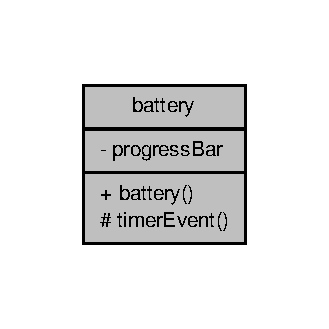
\includegraphics[width=158pt]{classbattery__coll__graph}
\end{center}
\end{figure}
\subsection*{Public Member Functions}
\begin{DoxyCompactItemize}
\item 
\hyperlink{classbattery_a5fa1ba3fd447e78847e63f5733e157af}{battery} (Q\-Widget $\ast$parent=0)
\begin{DoxyCompactList}\small\item\em Constructeur. \end{DoxyCompactList}\end{DoxyCompactItemize}
\subsection*{Protected Member Functions}
\begin{DoxyCompactItemize}
\item 
void \hyperlink{classbattery_a22c4b7b9932a588d61fde097aa7a91a5}{timer\-Event} (Q\-Timer\-Event $\ast$event)
\begin{DoxyCompactList}\small\item\em Timer. \end{DoxyCompactList}\end{DoxyCompactItemize}
\subsection*{Private Attributes}
\begin{DoxyCompactItemize}
\item 
Q\-Progress\-Bar $\ast$ \hyperlink{classbattery_af0da6fea5bb4d46f1e4bd9b3abe970ed}{progress\-Bar}
\end{DoxyCompactItemize}


\subsection{Detailed Description}


Definition at line 15 of file battery.\-h.



\subsection{Constructor \& Destructor Documentation}
\hypertarget{classbattery_a5fa1ba3fd447e78847e63f5733e157af}{\index{battery@{battery}!battery@{battery}}
\index{battery@{battery}!battery@{battery}}
\subsubsection[{battery}]{\setlength{\rightskip}{0pt plus 5cm}battery\-::battery (
\begin{DoxyParamCaption}
\item[{Q\-Widget $\ast$}]{parent = {\ttfamily 0}}
\end{DoxyParamCaption}
)\hspace{0.3cm}{\ttfamily [explicit]}}}\label{classbattery_a5fa1ba3fd447e78847e63f5733e157af}


Constructeur. 

Permet la déclaration et la définition de de la taille de la progress\-Bar 
\begin{DoxyParams}{Parameters}
{\em Q\-Widget} & $\ast$parent \\
\hline
\end{DoxyParams}


Definition at line 19 of file battery.\-cpp.



References progress\-Bar.


\begin{DoxyCode}
                                :
    QMainWindow(parent)
\{
    \hyperlink{classbattery_af0da6fea5bb4d46f1e4bd9b3abe970ed}{progressBar} = \textcolor{keyword}{new} QProgressBar(\textcolor{keyword}{this});
    \hyperlink{classbattery_af0da6fea5bb4d46f1e4bd9b3abe970ed}{progressBar}->setGeometry(10, 10, 85, 20);
    startTimer(200);
\}
\end{DoxyCode}


\subsection{Member Function Documentation}
\hypertarget{classbattery_a22c4b7b9932a588d61fde097aa7a91a5}{\index{battery@{battery}!timer\-Event@{timer\-Event}}
\index{timer\-Event@{timer\-Event}!battery@{battery}}
\subsubsection[{timer\-Event}]{\setlength{\rightskip}{0pt plus 5cm}void battery\-::timer\-Event (
\begin{DoxyParamCaption}
\item[{Q\-Timer\-Event $\ast$}]{event}
\end{DoxyParamCaption}
)\hspace{0.3cm}{\ttfamily [protected]}}}\label{classbattery_a22c4b7b9932a588d61fde097aa7a91a5}


Timer. 

Permet le rafraichissement des valeurs pour l'affichage de l'état des batteries du drone et de la base. 
\begin{DoxyParams}{Parameters}
{\em Q\-Timer\-Event} & $\ast$event \\
\hline
\end{DoxyParams}


Definition at line 33 of file battery.\-cpp.



References progress\-Bar.


\begin{DoxyCode}
\{
    \textcolor{comment}{/*QFile fichier("/home/estei/projet/fonctionnel/GPS/niveauBatterie.txt");*/}
                                                    \textcolor{comment}{/* Récupère la valeur contenue
       dans le répertoire /temp/LOG pour la batterie de la base */}
    \textcolor{comment}{/* POUR L'INTEGRATION */}
    QFile fichier(\textcolor{stringliteral}{"/tmp/LOG"});
    QString ligne;
    QTextStream flux(&fichier);

    \textcolor{keywordflow}{if}(fichier.open(QIODevice::ReadOnly | QIODevice::Text))
    \{
        \textcolor{keywordflow}{while}(!flux.atEnd())
        \{
            ligne = fichier.readLine();
        \}
        fichier.close();
    \}
    \textcolor{keywordflow}{else}
        ligne = \textcolor{stringliteral}{"Impossible d'ouvrir le fichier !"};
    \hyperlink{classbattery_af0da6fea5bb4d46f1e4bd9b3abe970ed}{progressBar}->setValue(ligne.toInt());                           
              \textcolor{comment}{/* Fixe la valeur de la progressBar avec la valeur récupérée */}
    \textcolor{keywordflow}{if}(ligne.toInt() >= 50)                                                 \textcolor{comment}{/*
       Si la valeur est supérieure ou égale à 50%, elle est de couleur verte */}
        setStyleSheet(\textcolor{stringliteral}{"QProgressBar::chunk\{background-color:green\}"});
    \textcolor{keywordflow}{if}(ligne.toInt() < 50)                                                  \textcolor{comment}{/*
       Si la valeur est inférieure à 50%, elle est de couleur orange */}
        setStyleSheet(\textcolor{stringliteral}{"QProgressBar::chunk\{background-color:orange\}"});
    \textcolor{keywordflow}{if}(ligne.toInt() < 20 )                                                 \textcolor{comment}{/*
       Si la valeur est inférieure à 20%, elle est de couleur rouge */}
        setStyleSheet(\textcolor{stringliteral}{"QProgressBar::chunk\{background-color:red\}"});


\}
\end{DoxyCode}


\subsection{Member Data Documentation}
\hypertarget{classbattery_af0da6fea5bb4d46f1e4bd9b3abe970ed}{\index{battery@{battery}!progress\-Bar@{progress\-Bar}}
\index{progress\-Bar@{progress\-Bar}!battery@{battery}}
\subsubsection[{progress\-Bar}]{\setlength{\rightskip}{0pt plus 5cm}Q\-Progress\-Bar$\ast$ battery\-::progress\-Bar\hspace{0.3cm}{\ttfamily [private]}}}\label{classbattery_af0da6fea5bb4d46f1e4bd9b3abe970ed}


Definition at line 24 of file battery.\-h.



Referenced by battery(), and timer\-Event().



The documentation for this class was generated from the following files\-:\begin{DoxyCompactItemize}
\item 
\hyperlink{battery_8h}{battery.\-h}\item 
\hyperlink{battery_8cpp}{battery.\-cpp}\end{DoxyCompactItemize}

\hypertarget{classCameraWidget}{\section{Camera\-Widget Class Reference}
\label{classCameraWidget}\index{Camera\-Widget@{Camera\-Widget}}
}


{\ttfamily \#include \char`\"{}camerawidget.\-h\char`\"{}}



Collaboration diagram for Camera\-Widget\-:\nopagebreak
\begin{figure}[H]
\begin{center}
\leavevmode
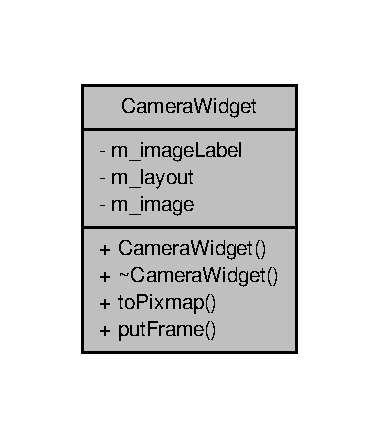
\includegraphics[width=182pt]{classCameraWidget__coll__graph}
\end{center}
\end{figure}
\subsection*{Public Member Functions}
\begin{DoxyCompactItemize}
\item 
\hyperlink{classCameraWidget_a637ffd88fb213dad01dfa7294248029e}{Camera\-Widget} (Q\-Widget $\ast$parent=0)
\begin{DoxyCompactList}\small\item\em Constructeur. \end{DoxyCompactList}\item 
\hyperlink{classCameraWidget_a434ed0e3355c13cd4a51eba0dfcfa66a}{$\sim$\-Camera\-Widget} (void)
\begin{DoxyCompactList}\small\item\em Destructeur. \end{DoxyCompactList}\item 
Q\-Pixmap \hyperlink{classCameraWidget_a349b27ddfbcd67ae055f56e51ffe3e44}{to\-Pixmap} (Ipl\-Image $\ast$)
\begin{DoxyCompactList}\small\item\em Conversion d'image. \end{DoxyCompactList}\item 
void \hyperlink{classCameraWidget_a9ef3bc90490e18855ac24f29cc5cb20f}{put\-Frame} (Ipl\-Image $\ast$)
\begin{DoxyCompactList}\small\item\em Placement d'image. \end{DoxyCompactList}\end{DoxyCompactItemize}
\subsection*{Private Attributes}
\begin{DoxyCompactItemize}
\item 
Q\-Label $\ast$ \hyperlink{classCameraWidget_aca76b8be07d57c2d715a685768dfcbe6}{m\-\_\-image\-Label}
\item 
Q\-V\-Box\-Layout $\ast$ \hyperlink{classCameraWidget_a22be3fef82e8e5c1e125b280ec1434df}{m\-\_\-layout}
\item 
Q\-Image \hyperlink{classCameraWidget_a953550f36cf3dd234dd33e36f0e85e95}{m\-\_\-image}
\end{DoxyCompactItemize}


\subsection{Detailed Description}


Definition at line 21 of file camerawidget.\-h.



\subsection{Constructor \& Destructor Documentation}
\hypertarget{classCameraWidget_a637ffd88fb213dad01dfa7294248029e}{\index{Camera\-Widget@{Camera\-Widget}!Camera\-Widget@{Camera\-Widget}}
\index{Camera\-Widget@{Camera\-Widget}!CameraWidget@{Camera\-Widget}}
\subsubsection[{Camera\-Widget}]{\setlength{\rightskip}{0pt plus 5cm}Camera\-Widget\-::\-Camera\-Widget (
\begin{DoxyParamCaption}
\item[{Q\-Widget $\ast$}]{parent = {\ttfamily 0}}
\end{DoxyParamCaption}
)}}\label{classCameraWidget_a637ffd88fb213dad01dfa7294248029e}


Constructeur. 

Placement du label dans un layout. 
\begin{DoxyParams}{Parameters}
{\em Q\-Widget} & $\ast$parent \\
\hline
\end{DoxyParams}


Definition at line 17 of file camerawidget.\-cpp.



References m\-\_\-image, m\-\_\-image\-Label, and m\-\_\-layout.


\begin{DoxyCode}
    : QWidget(parent)
\{
    \hyperlink{classCameraWidget_a22be3fef82e8e5c1e125b280ec1434df}{m\_layout} = \textcolor{keyword}{new} QVBoxLayout;
    \hyperlink{classCameraWidget_aca76b8be07d57c2d715a685768dfcbe6}{m\_imageLabel} = \textcolor{keyword}{new} QLabel;

    QImage dummy(100, 100, QImage::Format\_RGB32);
    \hyperlink{classCameraWidget_a953550f36cf3dd234dd33e36f0e85e95}{m\_image} = dummy;

    \hyperlink{classCameraWidget_a22be3fef82e8e5c1e125b280ec1434df}{m\_layout}->addWidget(\hyperlink{classCameraWidget_aca76b8be07d57c2d715a685768dfcbe6}{m\_imageLabel});

    \textcolor{keywordflow}{for} (\textcolor{keywordtype}{int} x = 0; x < 100; x ++)
        \textcolor{keywordflow}{for} (\textcolor{keywordtype}{int} y =0; y < 100; y++)
            \hyperlink{classCameraWidget_a953550f36cf3dd234dd33e36f0e85e95}{m\_image}.setPixel(x,y,qRgb(x, y, y));

    \hyperlink{classCameraWidget_aca76b8be07d57c2d715a685768dfcbe6}{m\_imageLabel}->setPixmap(QPixmap::fromImage(\hyperlink{classCameraWidget_a953550f36cf3dd234dd33e36f0e85e95}{m\_image}));

    setLayout(\hyperlink{classCameraWidget_a22be3fef82e8e5c1e125b280ec1434df}{m\_layout});
\}
\end{DoxyCode}
\hypertarget{classCameraWidget_a434ed0e3355c13cd4a51eba0dfcfa66a}{\index{Camera\-Widget@{Camera\-Widget}!$\sim$\-Camera\-Widget@{$\sim$\-Camera\-Widget}}
\index{$\sim$\-Camera\-Widget@{$\sim$\-Camera\-Widget}!CameraWidget@{Camera\-Widget}}
\subsubsection[{$\sim$\-Camera\-Widget}]{\setlength{\rightskip}{0pt plus 5cm}Camera\-Widget\-::$\sim$\-Camera\-Widget (
\begin{DoxyParamCaption}
\item[{void}]{}
\end{DoxyParamCaption}
)}}\label{classCameraWidget_a434ed0e3355c13cd4a51eba0dfcfa66a}


Destructeur. 


\begin{DoxyParams}{Parameters}
{\em void} & \\
\hline
\end{DoxyParams}


Definition at line 42 of file camerawidget.\-cpp.


\begin{DoxyCode}
\{

\}
\end{DoxyCode}


\subsection{Member Function Documentation}
\hypertarget{classCameraWidget_a9ef3bc90490e18855ac24f29cc5cb20f}{\index{Camera\-Widget@{Camera\-Widget}!put\-Frame@{put\-Frame}}
\index{put\-Frame@{put\-Frame}!CameraWidget@{Camera\-Widget}}
\subsubsection[{put\-Frame}]{\setlength{\rightskip}{0pt plus 5cm}void Camera\-Widget\-::put\-Frame (
\begin{DoxyParamCaption}
\item[{Ipl\-Image $\ast$}]{image}
\end{DoxyParamCaption}
)}}\label{classCameraWidget_a9ef3bc90490e18855ac24f29cc5cb20f}


Placement d'image. 

Fonction qui permet le placement de l'image dans le label destiné à l'accueillir 
\begin{DoxyParams}{Parameters}
{\em Ipl\-Image} & $\ast$image \\
\hline
\end{DoxyParams}


Definition at line 53 of file camerawidget.\-cpp.



References m\-\_\-image\-Label, and to\-Pixmap().



Referenced by Main\-Window\-::timer\-Event().


\begin{DoxyCode}
\{
    \hyperlink{classCameraWidget_aca76b8be07d57c2d715a685768dfcbe6}{m\_imageLabel}->setPixmap(\hyperlink{classCameraWidget_a349b27ddfbcd67ae055f56e51ffe3e44}{toPixmap}(image));
\}
\end{DoxyCode}
\hypertarget{classCameraWidget_a349b27ddfbcd67ae055f56e51ffe3e44}{\index{Camera\-Widget@{Camera\-Widget}!to\-Pixmap@{to\-Pixmap}}
\index{to\-Pixmap@{to\-Pixmap}!CameraWidget@{Camera\-Widget}}
\subsubsection[{to\-Pixmap}]{\setlength{\rightskip}{0pt plus 5cm}Q\-Pixmap Camera\-Widget\-::to\-Pixmap (
\begin{DoxyParamCaption}
\item[{Ipl\-Image $\ast$}]{cvimage}
\end{DoxyParamCaption}
)}}\label{classCameraWidget_a349b27ddfbcd67ae055f56e51ffe3e44}


Conversion d'image. 

Fonction de conversion d'une Ipl\-Image en une Q\-Pixmap 
\begin{DoxyParams}{Parameters}
{\em Ipl\-Image} & $\ast$cvimage \\
\hline
\end{DoxyParams}
\begin{DoxyReturn}{Returns}
Q\-Pixmap 
\end{DoxyReturn}


Definition at line 65 of file camerawidget.\-cpp.



References m\-\_\-image.



Referenced by put\-Frame(), and Main\-Window\-::save\-Picture().


\begin{DoxyCode}
                                                \{
    \textcolor{keywordtype}{int} cvIndex, cvLineStart;

    \textcolor{keywordflow}{switch} (cvimage->depth) \{
        \textcolor{keywordflow}{case} IPL\_DEPTH\_8U:
            \textcolor{keywordflow}{switch} (cvimage->nChannels) \{
                \textcolor{keywordflow}{case} 3:
                    \textcolor{keywordflow}{if} ( (cvimage->width != \hyperlink{classCameraWidget_a953550f36cf3dd234dd33e36f0e85e95}{m\_image}.width()) || (cvimage
      ->height != \hyperlink{classCameraWidget_a953550f36cf3dd234dd33e36f0e85e95}{m\_image}.height()) ) \{
                        QImage temp(cvimage->width, cvimage->height, 
      QImage::Format\_RGB32);
                        \hyperlink{classCameraWidget_a953550f36cf3dd234dd33e36f0e85e95}{m\_image} = temp;
                    \}
                    cvIndex = 0; cvLineStart = 0;
                    \textcolor{keywordflow}{for} (\textcolor{keywordtype}{int} y = 0; y < cvimage->height; y++) \{
                        \textcolor{keywordtype}{unsigned} \textcolor{keywordtype}{char} red,green,blue;
                        cvIndex = cvLineStart;
                        \textcolor{keywordflow}{for} (\textcolor{keywordtype}{int} x = 0; x < cvimage->width; x++) \{
                            red = cvimage->imageData[cvIndex+2];
                            green = cvimage->imageData[cvIndex+1];
                            blue = cvimage->imageData[cvIndex+0];

                            \hyperlink{classCameraWidget_a953550f36cf3dd234dd33e36f0e85e95}{m\_image}.setPixel(x,y,qRgb(red, green, blue))
      ;
                            cvIndex += 3;
                        \}
                        cvLineStart += cvimage->widthStep;
                    \}
                    \textcolor{keywordflow}{break};

            \textcolor{keywordflow}{case} 1:
                \textcolor{keywordflow}{if} ( (cvimage->width != \hyperlink{classCameraWidget_a953550f36cf3dd234dd33e36f0e85e95}{m\_image}.width()) || (cvimage->
      height != \hyperlink{classCameraWidget_a953550f36cf3dd234dd33e36f0e85e95}{m\_image}.height()) ) \{
                    QImage temp(cvimage->width, cvimage->height, 
      QImage::Format\_RGB32);
                    \hyperlink{classCameraWidget_a953550f36cf3dd234dd33e36f0e85e95}{m\_image} = temp;
                \}
                cvIndex = 0; cvLineStart = 0;
                \textcolor{keywordflow}{for} (\textcolor{keywordtype}{int} y = 0; y < cvimage->height; y++) \{
                    \textcolor{keywordtype}{unsigned} \textcolor{keywordtype}{char} red,green,blue;
                    cvIndex = cvLineStart;
                    \textcolor{keywordflow}{for} (\textcolor{keywordtype}{int} x = 0; x < cvimage->width; x++) \{
                        red = cvimage->imageData[cvIndex+2];
                        green = cvimage->imageData[cvIndex+1];
                        blue = cvimage->imageData[cvIndex+0];

                        \hyperlink{classCameraWidget_a953550f36cf3dd234dd33e36f0e85e95}{m\_image}.setPixel(x,y,qRgb(red, green, blue));
                        cvIndex += 3;
                    \}
                    cvLineStart += cvimage->widthStep;
                \}
                \textcolor{keywordflow}{break};
                \textcolor{keywordflow}{default}:
                    qWarning(\textcolor{stringliteral}{"This number of channels is not supported\(\backslash\)n"});
                    \textcolor{keywordflow}{break};
            \}
            \textcolor{keywordflow}{break};
        \textcolor{keywordflow}{default}:
            qWarning(\textcolor{stringliteral}{"This type of IplImage is not implemented in QOpenCVWidget
      \(\backslash\)n"});
            \textcolor{keywordflow}{break};
    \}
    \textcolor{keywordflow}{return} QPixmap::fromImage(\hyperlink{classCameraWidget_a953550f36cf3dd234dd33e36f0e85e95}{m\_image});
\}
\end{DoxyCode}


\subsection{Member Data Documentation}
\hypertarget{classCameraWidget_a953550f36cf3dd234dd33e36f0e85e95}{\index{Camera\-Widget@{Camera\-Widget}!m\-\_\-image@{m\-\_\-image}}
\index{m\-\_\-image@{m\-\_\-image}!CameraWidget@{Camera\-Widget}}
\subsubsection[{m\-\_\-image}]{\setlength{\rightskip}{0pt plus 5cm}Q\-Image Camera\-Widget\-::m\-\_\-image\hspace{0.3cm}{\ttfamily [private]}}}\label{classCameraWidget_a953550f36cf3dd234dd33e36f0e85e95}


Definition at line 33 of file camerawidget.\-h.



Referenced by Camera\-Widget(), and to\-Pixmap().

\hypertarget{classCameraWidget_aca76b8be07d57c2d715a685768dfcbe6}{\index{Camera\-Widget@{Camera\-Widget}!m\-\_\-image\-Label@{m\-\_\-image\-Label}}
\index{m\-\_\-image\-Label@{m\-\_\-image\-Label}!CameraWidget@{Camera\-Widget}}
\subsubsection[{m\-\_\-image\-Label}]{\setlength{\rightskip}{0pt plus 5cm}Q\-Label$\ast$ Camera\-Widget\-::m\-\_\-image\-Label\hspace{0.3cm}{\ttfamily [private]}}}\label{classCameraWidget_aca76b8be07d57c2d715a685768dfcbe6}


Definition at line 31 of file camerawidget.\-h.



Referenced by Camera\-Widget(), and put\-Frame().

\hypertarget{classCameraWidget_a22be3fef82e8e5c1e125b280ec1434df}{\index{Camera\-Widget@{Camera\-Widget}!m\-\_\-layout@{m\-\_\-layout}}
\index{m\-\_\-layout@{m\-\_\-layout}!CameraWidget@{Camera\-Widget}}
\subsubsection[{m\-\_\-layout}]{\setlength{\rightskip}{0pt plus 5cm}Q\-V\-Box\-Layout$\ast$ Camera\-Widget\-::m\-\_\-layout\hspace{0.3cm}{\ttfamily [private]}}}\label{classCameraWidget_a22be3fef82e8e5c1e125b280ec1434df}


Definition at line 32 of file camerawidget.\-h.



Referenced by Camera\-Widget().



The documentation for this class was generated from the following files\-:\begin{DoxyCompactItemize}
\item 
\hyperlink{camerawidget_8h}{camerawidget.\-h}\item 
\hyperlink{camerawidget_8cpp}{camerawidget.\-cpp}\end{DoxyCompactItemize}

\hypertarget{structdroneBatteryData}{\section{drone\-Battery\-Data Struct Reference}
\label{structdroneBatteryData}\index{drone\-Battery\-Data@{drone\-Battery\-Data}}
}


{\ttfamily \#include \char`\"{}typdef\-Uart.\-h\char`\"{}}



Collaboration diagram for drone\-Battery\-Data\-:\nopagebreak
\begin{figure}[H]
\begin{center}
\leavevmode
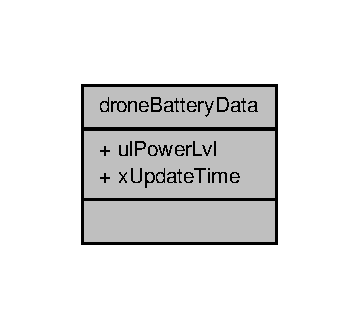
\includegraphics[width=172pt]{structdroneBatteryData__coll__graph}
\end{center}
\end{figure}
\subsection*{Public Attributes}
\begin{DoxyCompactItemize}
\item 
\hyperlink{typdefUart_8h_a435d1572bf3f880d55459d9805097f62}{uint32\-\_\-t} \hyperlink{structdroneBatteryData_a789c02e04e8c2e46989309ff33c44b1d}{ul\-Power\-Lvl}
\item 
\hyperlink{typdefUart_8h_ae9fa5e001303f1be1c0294f26cde8caf}{port\-Tick\-Type} \hyperlink{structdroneBatteryData_a52ebc5b82ebb0220cff03229eb9c660f}{x\-Update\-Time}
\end{DoxyCompactItemize}


\subsection{Detailed Description}


Definition at line 222 of file typdef\-Uart.\-h.



\subsection{Member Data Documentation}
\hypertarget{structdroneBatteryData_a789c02e04e8c2e46989309ff33c44b1d}{\index{drone\-Battery\-Data@{drone\-Battery\-Data}!ul\-Power\-Lvl@{ul\-Power\-Lvl}}
\index{ul\-Power\-Lvl@{ul\-Power\-Lvl}!droneBatteryData@{drone\-Battery\-Data}}
\subsubsection[{ul\-Power\-Lvl}]{\setlength{\rightskip}{0pt plus 5cm}{\bf uint32\-\_\-t} drone\-Battery\-Data\-::ul\-Power\-Lvl}}\label{structdroneBatteryData_a789c02e04e8c2e46989309ff33c44b1d}


Definition at line 224 of file typdef\-Uart.\-h.

\hypertarget{structdroneBatteryData_a52ebc5b82ebb0220cff03229eb9c660f}{\index{drone\-Battery\-Data@{drone\-Battery\-Data}!x\-Update\-Time@{x\-Update\-Time}}
\index{x\-Update\-Time@{x\-Update\-Time}!droneBatteryData@{drone\-Battery\-Data}}
\subsubsection[{x\-Update\-Time}]{\setlength{\rightskip}{0pt plus 5cm}{\bf port\-Tick\-Type} drone\-Battery\-Data\-::x\-Update\-Time}}\label{structdroneBatteryData_a52ebc5b82ebb0220cff03229eb9c660f}


Definition at line 226 of file typdef\-Uart.\-h.



The documentation for this struct was generated from the following file\-:\begin{DoxyCompactItemize}
\item 
\hyperlink{typdefUart_8h}{typdef\-Uart.\-h}\end{DoxyCompactItemize}

\hypertarget{structdroneConfig}{\section{drone\-Config Struct Reference}
\label{structdroneConfig}\index{drone\-Config@{drone\-Config}}
}


{\ttfamily \#include \char`\"{}typdef\-Uart.\-h\char`\"{}}



Collaboration diagram for drone\-Config\-:\nopagebreak
\begin{figure}[H]
\begin{center}
\leavevmode
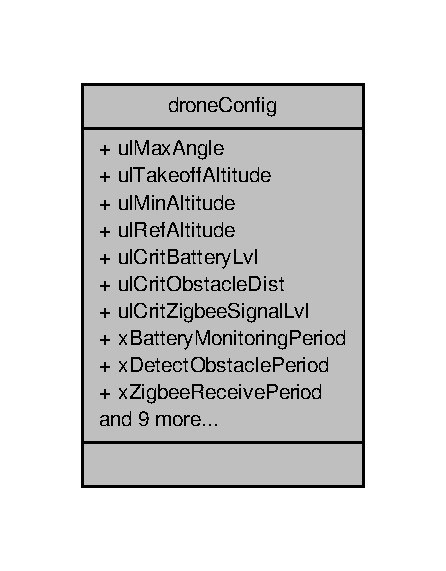
\includegraphics[width=214pt]{structdroneConfig__coll__graph}
\end{center}
\end{figure}
\subsection*{Public Attributes}
\begin{DoxyCompactItemize}
\item 
\hyperlink{typdefUart_8h_a435d1572bf3f880d55459d9805097f62}{uint32\-\_\-t} \hyperlink{structdroneConfig_a0f6ba8c7c50c247ef54fa48e0f7ef729}{ul\-Max\-Angle}
\item 
\hyperlink{typdefUart_8h_a435d1572bf3f880d55459d9805097f62}{uint32\-\_\-t} \hyperlink{structdroneConfig_a732c5a9d1af9eec7412c8a282109728a}{ul\-Takeoff\-Altitude}
\item 
\hyperlink{typdefUart_8h_a435d1572bf3f880d55459d9805097f62}{uint32\-\_\-t} \hyperlink{structdroneConfig_a93de26859c52f79b9801cf74e1e37add}{ul\-Min\-Altitude}
\item 
\hyperlink{typdefUart_8h_a435d1572bf3f880d55459d9805097f62}{uint32\-\_\-t} \hyperlink{structdroneConfig_a7d7f05ea8f93c206ce1a8a2fa868c587}{ul\-Ref\-Altitude}
\item 
\hyperlink{typdefUart_8h_a435d1572bf3f880d55459d9805097f62}{uint32\-\_\-t} \hyperlink{structdroneConfig_a4ec612c83c80eba7815c541307c9f619}{ul\-Crit\-Battery\-Lvl}
\item 
\hyperlink{typdefUart_8h_a435d1572bf3f880d55459d9805097f62}{uint32\-\_\-t} \hyperlink{structdroneConfig_a39b4ebfe2fad46f568b7a2953fc8f46d}{ul\-Crit\-Obstacle\-Dist}
\item 
\hyperlink{typdefUart_8h_a435d1572bf3f880d55459d9805097f62}{uint32\-\_\-t} \hyperlink{structdroneConfig_ace08c1c7161f782950192970d7a19d75}{ul\-Crit\-Zigbee\-Signal\-Lvl}
\item 
\hyperlink{typdefUart_8h_ae9fa5e001303f1be1c0294f26cde8caf}{port\-Tick\-Type} \hyperlink{structdroneConfig_afa883d29d2c43da22c11352af00ffb7b}{x\-Battery\-Monitoring\-Period}
\item 
\hyperlink{typdefUart_8h_ae9fa5e001303f1be1c0294f26cde8caf}{port\-Tick\-Type} \hyperlink{structdroneConfig_ac536a237bbb15769d731ec98495d7d97}{x\-Detect\-Obstacle\-Period}
\item 
\hyperlink{typdefUart_8h_ae9fa5e001303f1be1c0294f26cde8caf}{port\-Tick\-Type} \hyperlink{structdroneConfig_a8f16de66ac71b922d151ea165b9f4871}{x\-Zigbee\-Receive\-Period}
\item 
\hyperlink{typdefUart_8h_ae9fa5e001303f1be1c0294f26cde8caf}{port\-Tick\-Type} \hyperlink{structdroneConfig_a92f8e6403d9ca068830a44280239e551}{x\-Flight\-Ctrl\-Period}
\item 
\hyperlink{typdefUart_8h_ae9fa5e001303f1be1c0294f26cde8caf}{port\-Tick\-Type} \hyperlink{structdroneConfig_ae0b978b5906545132a1a1a37c3ca4907}{x\-G\-P\-S\-Receive\-Period}
\item 
\hyperlink{typdefUart_8h_ae9fa5e001303f1be1c0294f26cde8caf}{port\-Tick\-Type} \hyperlink{structdroneConfig_a7035d86cd38b594b1dbb98a80620ed22}{x\-Video\-Toggle\-Period}
\item 
\hyperlink{typdefUart_8h_aba7bc1797add20fe3efdf37ced1182c5}{uint8\-\_\-t} \hyperlink{structdroneConfig_a9abfb72bb174ea001aa9cbe0e196fac7}{x\-I\-M\-U\-Data\-Timeout}
\item 
\hyperlink{typdefUart_8h_aba7bc1797add20fe3efdf37ced1182c5}{uint8\-\_\-t} \hyperlink{structdroneConfig_a2eee39829fa6406904f2853658554814}{x\-Zigbee\-Cmd\-Timeout}
\item 
\hyperlink{typdefUart_8h_aba7bc1797add20fe3efdf37ced1182c5}{uint8\-\_\-t} \hyperlink{structdroneConfig_a5708172eb0cdfd665ee9ba776168faa1}{x\-Zigbee\-Receive\-Timeout}
\item 
\hyperlink{typdefUart_8h_aba7bc1797add20fe3efdf37ced1182c5}{uint8\-\_\-t} \hyperlink{structdroneConfig_aa191e8867f3a6277d18a0f4379affb1b}{x\-Telemeter\-Timeout}
\item 
\hyperlink{typdefUart_8h_aba7bc1797add20fe3efdf37ced1182c5}{uint8\-\_\-t} \hyperlink{structdroneConfig_a30a59cf24e01d514b6d72c86deb1f02e}{x\-Battery\-Timeout}
\item 
\hyperlink{typdefUart_8h_aba7bc1797add20fe3efdf37ced1182c5}{uint8\-\_\-t} \hyperlink{structdroneConfig_ae272c4dd5a556fe40d2ea3105bf0aa96}{x\-G\-P\-S\-Timeout}
\end{DoxyCompactItemize}


\subsection{Detailed Description}


Definition at line 78 of file typdef\-Uart.\-h.



\subsection{Member Data Documentation}
\hypertarget{structdroneConfig_a4ec612c83c80eba7815c541307c9f619}{\index{drone\-Config@{drone\-Config}!ul\-Crit\-Battery\-Lvl@{ul\-Crit\-Battery\-Lvl}}
\index{ul\-Crit\-Battery\-Lvl@{ul\-Crit\-Battery\-Lvl}!droneConfig@{drone\-Config}}
\subsubsection[{ul\-Crit\-Battery\-Lvl}]{\setlength{\rightskip}{0pt plus 5cm}{\bf uint32\-\_\-t} drone\-Config\-::ul\-Crit\-Battery\-Lvl}}\label{structdroneConfig_a4ec612c83c80eba7815c541307c9f619}


Definition at line 90 of file typdef\-Uart.\-h.

\hypertarget{structdroneConfig_a39b4ebfe2fad46f568b7a2953fc8f46d}{\index{drone\-Config@{drone\-Config}!ul\-Crit\-Obstacle\-Dist@{ul\-Crit\-Obstacle\-Dist}}
\index{ul\-Crit\-Obstacle\-Dist@{ul\-Crit\-Obstacle\-Dist}!droneConfig@{drone\-Config}}
\subsubsection[{ul\-Crit\-Obstacle\-Dist}]{\setlength{\rightskip}{0pt plus 5cm}{\bf uint32\-\_\-t} drone\-Config\-::ul\-Crit\-Obstacle\-Dist}}\label{structdroneConfig_a39b4ebfe2fad46f568b7a2953fc8f46d}


Definition at line 92 of file typdef\-Uart.\-h.

\hypertarget{structdroneConfig_ace08c1c7161f782950192970d7a19d75}{\index{drone\-Config@{drone\-Config}!ul\-Crit\-Zigbee\-Signal\-Lvl@{ul\-Crit\-Zigbee\-Signal\-Lvl}}
\index{ul\-Crit\-Zigbee\-Signal\-Lvl@{ul\-Crit\-Zigbee\-Signal\-Lvl}!droneConfig@{drone\-Config}}
\subsubsection[{ul\-Crit\-Zigbee\-Signal\-Lvl}]{\setlength{\rightskip}{0pt plus 5cm}{\bf uint32\-\_\-t} drone\-Config\-::ul\-Crit\-Zigbee\-Signal\-Lvl}}\label{structdroneConfig_ace08c1c7161f782950192970d7a19d75}


Definition at line 94 of file typdef\-Uart.\-h.

\hypertarget{structdroneConfig_a0f6ba8c7c50c247ef54fa48e0f7ef729}{\index{drone\-Config@{drone\-Config}!ul\-Max\-Angle@{ul\-Max\-Angle}}
\index{ul\-Max\-Angle@{ul\-Max\-Angle}!droneConfig@{drone\-Config}}
\subsubsection[{ul\-Max\-Angle}]{\setlength{\rightskip}{0pt plus 5cm}{\bf uint32\-\_\-t} drone\-Config\-::ul\-Max\-Angle}}\label{structdroneConfig_a0f6ba8c7c50c247ef54fa48e0f7ef729}


Definition at line 82 of file typdef\-Uart.\-h.

\hypertarget{structdroneConfig_a93de26859c52f79b9801cf74e1e37add}{\index{drone\-Config@{drone\-Config}!ul\-Min\-Altitude@{ul\-Min\-Altitude}}
\index{ul\-Min\-Altitude@{ul\-Min\-Altitude}!droneConfig@{drone\-Config}}
\subsubsection[{ul\-Min\-Altitude}]{\setlength{\rightskip}{0pt plus 5cm}{\bf uint32\-\_\-t} drone\-Config\-::ul\-Min\-Altitude}}\label{structdroneConfig_a93de26859c52f79b9801cf74e1e37add}


Definition at line 86 of file typdef\-Uart.\-h.

\hypertarget{structdroneConfig_a7d7f05ea8f93c206ce1a8a2fa868c587}{\index{drone\-Config@{drone\-Config}!ul\-Ref\-Altitude@{ul\-Ref\-Altitude}}
\index{ul\-Ref\-Altitude@{ul\-Ref\-Altitude}!droneConfig@{drone\-Config}}
\subsubsection[{ul\-Ref\-Altitude}]{\setlength{\rightskip}{0pt plus 5cm}{\bf uint32\-\_\-t} drone\-Config\-::ul\-Ref\-Altitude}}\label{structdroneConfig_a7d7f05ea8f93c206ce1a8a2fa868c587}


Definition at line 88 of file typdef\-Uart.\-h.

\hypertarget{structdroneConfig_a732c5a9d1af9eec7412c8a282109728a}{\index{drone\-Config@{drone\-Config}!ul\-Takeoff\-Altitude@{ul\-Takeoff\-Altitude}}
\index{ul\-Takeoff\-Altitude@{ul\-Takeoff\-Altitude}!droneConfig@{drone\-Config}}
\subsubsection[{ul\-Takeoff\-Altitude}]{\setlength{\rightskip}{0pt plus 5cm}{\bf uint32\-\_\-t} drone\-Config\-::ul\-Takeoff\-Altitude}}\label{structdroneConfig_a732c5a9d1af9eec7412c8a282109728a}


Definition at line 84 of file typdef\-Uart.\-h.

\hypertarget{structdroneConfig_afa883d29d2c43da22c11352af00ffb7b}{\index{drone\-Config@{drone\-Config}!x\-Battery\-Monitoring\-Period@{x\-Battery\-Monitoring\-Period}}
\index{x\-Battery\-Monitoring\-Period@{x\-Battery\-Monitoring\-Period}!droneConfig@{drone\-Config}}
\subsubsection[{x\-Battery\-Monitoring\-Period}]{\setlength{\rightskip}{0pt plus 5cm}{\bf port\-Tick\-Type} drone\-Config\-::x\-Battery\-Monitoring\-Period}}\label{structdroneConfig_afa883d29d2c43da22c11352af00ffb7b}


Definition at line 96 of file typdef\-Uart.\-h.

\hypertarget{structdroneConfig_a30a59cf24e01d514b6d72c86deb1f02e}{\index{drone\-Config@{drone\-Config}!x\-Battery\-Timeout@{x\-Battery\-Timeout}}
\index{x\-Battery\-Timeout@{x\-Battery\-Timeout}!droneConfig@{drone\-Config}}
\subsubsection[{x\-Battery\-Timeout}]{\setlength{\rightskip}{0pt plus 5cm}{\bf uint8\-\_\-t} drone\-Config\-::x\-Battery\-Timeout}}\label{structdroneConfig_a30a59cf24e01d514b6d72c86deb1f02e}


Definition at line 108 of file typdef\-Uart.\-h.

\hypertarget{structdroneConfig_ac536a237bbb15769d731ec98495d7d97}{\index{drone\-Config@{drone\-Config}!x\-Detect\-Obstacle\-Period@{x\-Detect\-Obstacle\-Period}}
\index{x\-Detect\-Obstacle\-Period@{x\-Detect\-Obstacle\-Period}!droneConfig@{drone\-Config}}
\subsubsection[{x\-Detect\-Obstacle\-Period}]{\setlength{\rightskip}{0pt plus 5cm}{\bf port\-Tick\-Type} drone\-Config\-::x\-Detect\-Obstacle\-Period}}\label{structdroneConfig_ac536a237bbb15769d731ec98495d7d97}


Definition at line 97 of file typdef\-Uart.\-h.

\hypertarget{structdroneConfig_a92f8e6403d9ca068830a44280239e551}{\index{drone\-Config@{drone\-Config}!x\-Flight\-Ctrl\-Period@{x\-Flight\-Ctrl\-Period}}
\index{x\-Flight\-Ctrl\-Period@{x\-Flight\-Ctrl\-Period}!droneConfig@{drone\-Config}}
\subsubsection[{x\-Flight\-Ctrl\-Period}]{\setlength{\rightskip}{0pt plus 5cm}{\bf port\-Tick\-Type} drone\-Config\-::x\-Flight\-Ctrl\-Period}}\label{structdroneConfig_a92f8e6403d9ca068830a44280239e551}


Definition at line 100 of file typdef\-Uart.\-h.

\hypertarget{structdroneConfig_ae0b978b5906545132a1a1a37c3ca4907}{\index{drone\-Config@{drone\-Config}!x\-G\-P\-S\-Receive\-Period@{x\-G\-P\-S\-Receive\-Period}}
\index{x\-G\-P\-S\-Receive\-Period@{x\-G\-P\-S\-Receive\-Period}!droneConfig@{drone\-Config}}
\subsubsection[{x\-G\-P\-S\-Receive\-Period}]{\setlength{\rightskip}{0pt plus 5cm}{\bf port\-Tick\-Type} drone\-Config\-::x\-G\-P\-S\-Receive\-Period}}\label{structdroneConfig_ae0b978b5906545132a1a1a37c3ca4907}


Definition at line 101 of file typdef\-Uart.\-h.

\hypertarget{structdroneConfig_ae272c4dd5a556fe40d2ea3105bf0aa96}{\index{drone\-Config@{drone\-Config}!x\-G\-P\-S\-Timeout@{x\-G\-P\-S\-Timeout}}
\index{x\-G\-P\-S\-Timeout@{x\-G\-P\-S\-Timeout}!droneConfig@{drone\-Config}}
\subsubsection[{x\-G\-P\-S\-Timeout}]{\setlength{\rightskip}{0pt plus 5cm}{\bf uint8\-\_\-t} drone\-Config\-::x\-G\-P\-S\-Timeout}}\label{structdroneConfig_ae272c4dd5a556fe40d2ea3105bf0aa96}


Definition at line 109 of file typdef\-Uart.\-h.

\hypertarget{structdroneConfig_a9abfb72bb174ea001aa9cbe0e196fac7}{\index{drone\-Config@{drone\-Config}!x\-I\-M\-U\-Data\-Timeout@{x\-I\-M\-U\-Data\-Timeout}}
\index{x\-I\-M\-U\-Data\-Timeout@{x\-I\-M\-U\-Data\-Timeout}!droneConfig@{drone\-Config}}
\subsubsection[{x\-I\-M\-U\-Data\-Timeout}]{\setlength{\rightskip}{0pt plus 5cm}{\bf uint8\-\_\-t} drone\-Config\-::x\-I\-M\-U\-Data\-Timeout}}\label{structdroneConfig_a9abfb72bb174ea001aa9cbe0e196fac7}


Definition at line 104 of file typdef\-Uart.\-h.

\hypertarget{structdroneConfig_aa191e8867f3a6277d18a0f4379affb1b}{\index{drone\-Config@{drone\-Config}!x\-Telemeter\-Timeout@{x\-Telemeter\-Timeout}}
\index{x\-Telemeter\-Timeout@{x\-Telemeter\-Timeout}!droneConfig@{drone\-Config}}
\subsubsection[{x\-Telemeter\-Timeout}]{\setlength{\rightskip}{0pt plus 5cm}{\bf uint8\-\_\-t} drone\-Config\-::x\-Telemeter\-Timeout}}\label{structdroneConfig_aa191e8867f3a6277d18a0f4379affb1b}


Definition at line 107 of file typdef\-Uart.\-h.

\hypertarget{structdroneConfig_a7035d86cd38b594b1dbb98a80620ed22}{\index{drone\-Config@{drone\-Config}!x\-Video\-Toggle\-Period@{x\-Video\-Toggle\-Period}}
\index{x\-Video\-Toggle\-Period@{x\-Video\-Toggle\-Period}!droneConfig@{drone\-Config}}
\subsubsection[{x\-Video\-Toggle\-Period}]{\setlength{\rightskip}{0pt plus 5cm}{\bf port\-Tick\-Type} drone\-Config\-::x\-Video\-Toggle\-Period}}\label{structdroneConfig_a7035d86cd38b594b1dbb98a80620ed22}


Definition at line 102 of file typdef\-Uart.\-h.

\hypertarget{structdroneConfig_a2eee39829fa6406904f2853658554814}{\index{drone\-Config@{drone\-Config}!x\-Zigbee\-Cmd\-Timeout@{x\-Zigbee\-Cmd\-Timeout}}
\index{x\-Zigbee\-Cmd\-Timeout@{x\-Zigbee\-Cmd\-Timeout}!droneConfig@{drone\-Config}}
\subsubsection[{x\-Zigbee\-Cmd\-Timeout}]{\setlength{\rightskip}{0pt plus 5cm}{\bf uint8\-\_\-t} drone\-Config\-::x\-Zigbee\-Cmd\-Timeout}}\label{structdroneConfig_a2eee39829fa6406904f2853658554814}


Definition at line 105 of file typdef\-Uart.\-h.

\hypertarget{structdroneConfig_a8f16de66ac71b922d151ea165b9f4871}{\index{drone\-Config@{drone\-Config}!x\-Zigbee\-Receive\-Period@{x\-Zigbee\-Receive\-Period}}
\index{x\-Zigbee\-Receive\-Period@{x\-Zigbee\-Receive\-Period}!droneConfig@{drone\-Config}}
\subsubsection[{x\-Zigbee\-Receive\-Period}]{\setlength{\rightskip}{0pt plus 5cm}{\bf port\-Tick\-Type} drone\-Config\-::x\-Zigbee\-Receive\-Period}}\label{structdroneConfig_a8f16de66ac71b922d151ea165b9f4871}


Definition at line 98 of file typdef\-Uart.\-h.

\hypertarget{structdroneConfig_a5708172eb0cdfd665ee9ba776168faa1}{\index{drone\-Config@{drone\-Config}!x\-Zigbee\-Receive\-Timeout@{x\-Zigbee\-Receive\-Timeout}}
\index{x\-Zigbee\-Receive\-Timeout@{x\-Zigbee\-Receive\-Timeout}!droneConfig@{drone\-Config}}
\subsubsection[{x\-Zigbee\-Receive\-Timeout}]{\setlength{\rightskip}{0pt plus 5cm}{\bf uint8\-\_\-t} drone\-Config\-::x\-Zigbee\-Receive\-Timeout}}\label{structdroneConfig_a5708172eb0cdfd665ee9ba776168faa1}


Definition at line 106 of file typdef\-Uart.\-h.



The documentation for this struct was generated from the following file\-:\begin{DoxyCompactItemize}
\item 
\hyperlink{typdefUart_8h}{typdef\-Uart.\-h}\end{DoxyCompactItemize}

\hypertarget{structdroneGPSData}{\section{drone\-G\-P\-S\-Data Struct Reference}
\label{structdroneGPSData}\index{drone\-G\-P\-S\-Data@{drone\-G\-P\-S\-Data}}
}


{\ttfamily \#include \char`\"{}typdef\-Uart.\-h\char`\"{}}



Collaboration diagram for drone\-G\-P\-S\-Data\-:\nopagebreak
\begin{figure}[H]
\begin{center}
\leavevmode
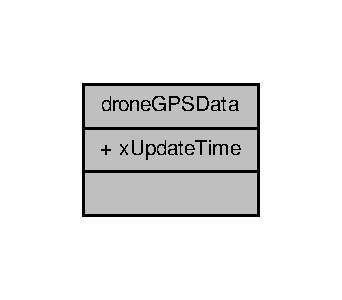
\includegraphics[width=164pt]{structdroneGPSData__coll__graph}
\end{center}
\end{figure}
\subsection*{Public Attributes}
\begin{DoxyCompactItemize}
\item 
\hyperlink{typdefUart_8h_ae9fa5e001303f1be1c0294f26cde8caf}{port\-Tick\-Type} \hyperlink{structdroneGPSData_a70d6916fb0e0d02ee97ee4208cafbbed}{x\-Update\-Time}
\end{DoxyCompactItemize}


\subsection{Detailed Description}


Definition at line 202 of file typdef\-Uart.\-h.



\subsection{Member Data Documentation}
\hypertarget{structdroneGPSData_a70d6916fb0e0d02ee97ee4208cafbbed}{\index{drone\-G\-P\-S\-Data@{drone\-G\-P\-S\-Data}!x\-Update\-Time@{x\-Update\-Time}}
\index{x\-Update\-Time@{x\-Update\-Time}!droneGPSData@{drone\-G\-P\-S\-Data}}
\subsubsection[{x\-Update\-Time}]{\setlength{\rightskip}{0pt plus 5cm}{\bf port\-Tick\-Type} drone\-G\-P\-S\-Data\-::x\-Update\-Time}}\label{structdroneGPSData_a70d6916fb0e0d02ee97ee4208cafbbed}


Definition at line 207 of file typdef\-Uart.\-h.



The documentation for this struct was generated from the following file\-:\begin{DoxyCompactItemize}
\item 
\hyperlink{typdefUart_8h}{typdef\-Uart.\-h}\end{DoxyCompactItemize}

\hypertarget{structdroneIMUData}{\section{drone\-I\-M\-U\-Data Struct Reference}
\label{structdroneIMUData}\index{drone\-I\-M\-U\-Data@{drone\-I\-M\-U\-Data}}
}


{\ttfamily \#include \char`\"{}typdef\-Uart.\-h\char`\"{}}



Collaboration diagram for drone\-I\-M\-U\-Data\-:\nopagebreak
\begin{figure}[H]
\begin{center}
\leavevmode
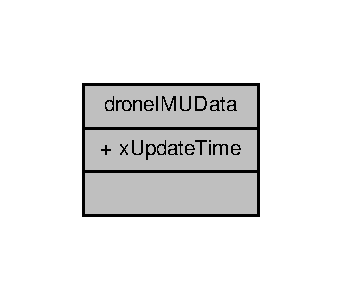
\includegraphics[width=164pt]{structdroneIMUData__coll__graph}
\end{center}
\end{figure}
\subsection*{Public Attributes}
\begin{DoxyCompactItemize}
\item 
\hyperlink{typdefUart_8h_ae9fa5e001303f1be1c0294f26cde8caf}{port\-Tick\-Type} \hyperlink{structdroneIMUData_a0ae68e4b692508cf64953adcb12443e1}{x\-Update\-Time}
\end{DoxyCompactItemize}


\subsection{Detailed Description}


Definition at line 195 of file typdef\-Uart.\-h.



\subsection{Member Data Documentation}
\hypertarget{structdroneIMUData_a0ae68e4b692508cf64953adcb12443e1}{\index{drone\-I\-M\-U\-Data@{drone\-I\-M\-U\-Data}!x\-Update\-Time@{x\-Update\-Time}}
\index{x\-Update\-Time@{x\-Update\-Time}!droneIMUData@{drone\-I\-M\-U\-Data}}
\subsubsection[{x\-Update\-Time}]{\setlength{\rightskip}{0pt plus 5cm}{\bf port\-Tick\-Type} drone\-I\-M\-U\-Data\-::x\-Update\-Time}}\label{structdroneIMUData_a0ae68e4b692508cf64953adcb12443e1}


Definition at line 199 of file typdef\-Uart.\-h.



The documentation for this struct was generated from the following file\-:\begin{DoxyCompactItemize}
\item 
\hyperlink{typdefUart_8h}{typdef\-Uart.\-h}\end{DoxyCompactItemize}

\hypertarget{structdroneState}{\section{drone\-State Struct Reference}
\label{structdroneState}\index{drone\-State@{drone\-State}}
}


{\ttfamily \#include \char`\"{}typdef\-Uart.\-h\char`\"{}}



Collaboration diagram for drone\-State\-:\nopagebreak
\begin{figure}[H]
\begin{center}
\leavevmode
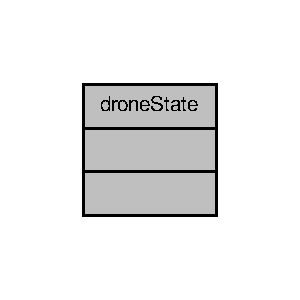
\includegraphics[width=144pt]{structdroneState__coll__graph}
\end{center}
\end{figure}


\subsection{Detailed Description}


Definition at line 185 of file typdef\-Uart.\-h.



The documentation for this struct was generated from the following file\-:\begin{DoxyCompactItemize}
\item 
\hyperlink{typdefUart_8h}{typdef\-Uart.\-h}\end{DoxyCompactItemize}

\hypertarget{structdroneTelemeterData}{\section{drone\-Telemeter\-Data Struct Reference}
\label{structdroneTelemeterData}\index{drone\-Telemeter\-Data@{drone\-Telemeter\-Data}}
}


{\ttfamily \#include \char`\"{}typdef\-Uart.\-h\char`\"{}}



Collaboration diagram for drone\-Telemeter\-Data\-:\nopagebreak
\begin{figure}[H]
\begin{center}
\leavevmode
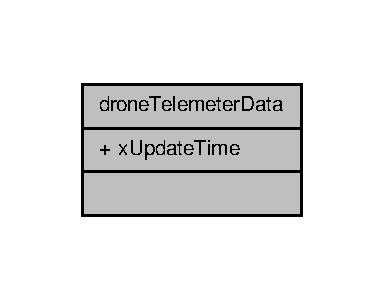
\includegraphics[width=184pt]{structdroneTelemeterData__coll__graph}
\end{center}
\end{figure}
\subsection*{Public Attributes}
\begin{DoxyCompactItemize}
\item 
\hyperlink{typdefUart_8h_ae9fa5e001303f1be1c0294f26cde8caf}{port\-Tick\-Type} \hyperlink{structdroneTelemeterData_ae1463929a7d9d3b5ef29137e92472f31}{x\-Update\-Time}
\end{DoxyCompactItemize}


\subsection{Detailed Description}


Definition at line 214 of file typdef\-Uart.\-h.



\subsection{Member Data Documentation}
\hypertarget{structdroneTelemeterData_ae1463929a7d9d3b5ef29137e92472f31}{\index{drone\-Telemeter\-Data@{drone\-Telemeter\-Data}!x\-Update\-Time@{x\-Update\-Time}}
\index{x\-Update\-Time@{x\-Update\-Time}!droneTelemeterData@{drone\-Telemeter\-Data}}
\subsubsection[{x\-Update\-Time}]{\setlength{\rightskip}{0pt plus 5cm}{\bf port\-Tick\-Type} drone\-Telemeter\-Data\-::x\-Update\-Time}}\label{structdroneTelemeterData_ae1463929a7d9d3b5ef29137e92472f31}


Definition at line 219 of file typdef\-Uart.\-h.



The documentation for this struct was generated from the following file\-:\begin{DoxyCompactItemize}
\item 
\hyperlink{typdefUart_8h}{typdef\-Uart.\-h}\end{DoxyCompactItemize}

\hypertarget{structflightCommand}{\section{flight\-Command Struct Reference}
\label{structflightCommand}\index{flight\-Command@{flight\-Command}}
}


{\ttfamily \#include \char`\"{}typdef\-Uart.\-h\char`\"{}}



Collaboration diagram for flight\-Command\-:\nopagebreak
\begin{figure}[H]
\begin{center}
\leavevmode
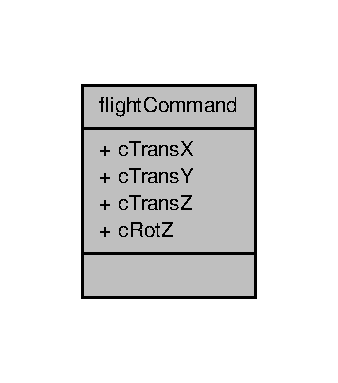
\includegraphics[width=162pt]{structflightCommand__coll__graph}
\end{center}
\end{figure}
\subsection*{Public Attributes}
\begin{DoxyCompactItemize}
\item 
int8\-\_\-t \hyperlink{structflightCommand_af700666e91aa7b7d619640bc75b9b907}{c\-Trans\-X}
\item 
int8\-\_\-t \hyperlink{structflightCommand_a4ec008f3e964d4e8ff8f700e4ec8d54a}{c\-Trans\-Y}
\item 
int8\-\_\-t \hyperlink{structflightCommand_abe6fac04c37189e2310de28de7df01d0}{c\-Trans\-Z}
\item 
int8\-\_\-t \hyperlink{structflightCommand_a8747d9907a0b26163b4fead3712797eb}{c\-Rot\-Z}
\end{DoxyCompactItemize}


\subsection{Detailed Description}


Definition at line 114 of file typdef\-Uart.\-h.



\subsection{Member Data Documentation}
\hypertarget{structflightCommand_a8747d9907a0b26163b4fead3712797eb}{\index{flight\-Command@{flight\-Command}!c\-Rot\-Z@{c\-Rot\-Z}}
\index{c\-Rot\-Z@{c\-Rot\-Z}!flightCommand@{flight\-Command}}
\subsubsection[{c\-Rot\-Z}]{\setlength{\rightskip}{0pt plus 5cm}int8\-\_\-t flight\-Command\-::c\-Rot\-Z}}\label{structflightCommand_a8747d9907a0b26163b4fead3712797eb}


Definition at line 121 of file typdef\-Uart.\-h.

\hypertarget{structflightCommand_af700666e91aa7b7d619640bc75b9b907}{\index{flight\-Command@{flight\-Command}!c\-Trans\-X@{c\-Trans\-X}}
\index{c\-Trans\-X@{c\-Trans\-X}!flightCommand@{flight\-Command}}
\subsubsection[{c\-Trans\-X}]{\setlength{\rightskip}{0pt plus 5cm}int8\-\_\-t flight\-Command\-::c\-Trans\-X}}\label{structflightCommand_af700666e91aa7b7d619640bc75b9b907}


Definition at line 117 of file typdef\-Uart.\-h.

\hypertarget{structflightCommand_a4ec008f3e964d4e8ff8f700e4ec8d54a}{\index{flight\-Command@{flight\-Command}!c\-Trans\-Y@{c\-Trans\-Y}}
\index{c\-Trans\-Y@{c\-Trans\-Y}!flightCommand@{flight\-Command}}
\subsubsection[{c\-Trans\-Y}]{\setlength{\rightskip}{0pt plus 5cm}int8\-\_\-t flight\-Command\-::c\-Trans\-Y}}\label{structflightCommand_a4ec008f3e964d4e8ff8f700e4ec8d54a}


Definition at line 118 of file typdef\-Uart.\-h.

\hypertarget{structflightCommand_abe6fac04c37189e2310de28de7df01d0}{\index{flight\-Command@{flight\-Command}!c\-Trans\-Z@{c\-Trans\-Z}}
\index{c\-Trans\-Z@{c\-Trans\-Z}!flightCommand@{flight\-Command}}
\subsubsection[{c\-Trans\-Z}]{\setlength{\rightskip}{0pt plus 5cm}int8\-\_\-t flight\-Command\-::c\-Trans\-Z}}\label{structflightCommand_abe6fac04c37189e2310de28de7df01d0}


Definition at line 119 of file typdef\-Uart.\-h.



The documentation for this struct was generated from the following file\-:\begin{DoxyCompactItemize}
\item 
\hyperlink{typdefUart_8h}{typdef\-Uart.\-h}\end{DoxyCompactItemize}

\hypertarget{classLightMaps}{\section{Light\-Maps Class Reference}
\label{classLightMaps}\index{Light\-Maps@{Light\-Maps}}
}


{\ttfamily \#include \char`\"{}lightmaps.\-h\char`\"{}}



Collaboration diagram for Light\-Maps\-:\nopagebreak
\begin{figure}[H]
\begin{center}
\leavevmode
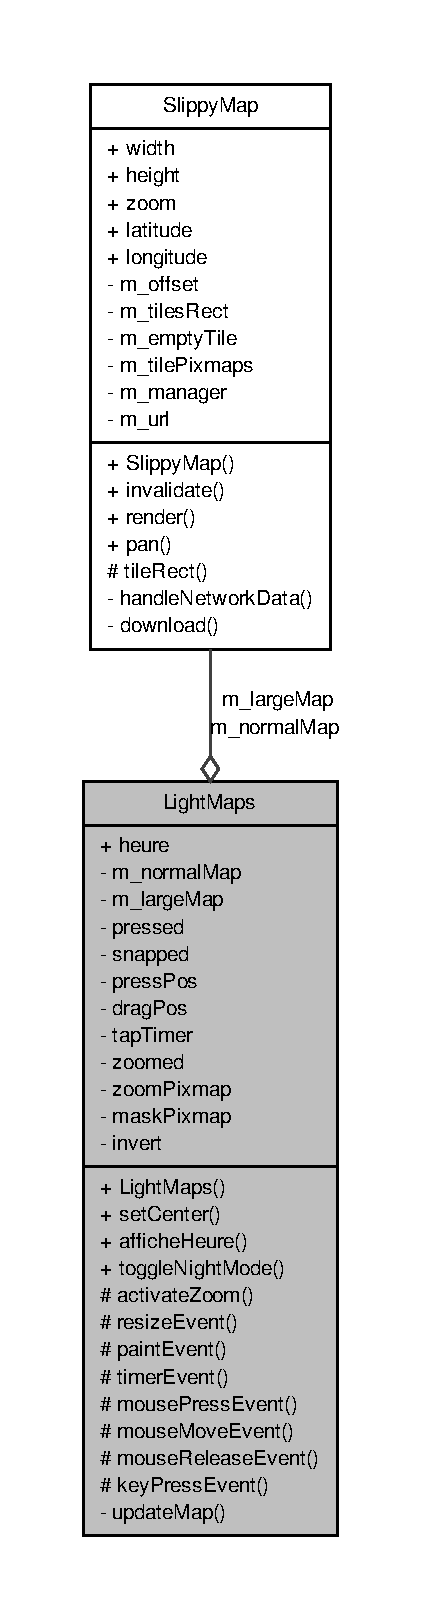
\includegraphics[height=550pt]{classLightMaps__coll__graph}
\end{center}
\end{figure}
\subsection*{Public Slots}
\begin{DoxyCompactItemize}
\item 
void \hyperlink{classLightMaps_a231905fb3ab4d3d488a64f3ac3bba7a3}{toggle\-Night\-Mode} ()
\end{DoxyCompactItemize}
\subsection*{Public Member Functions}
\begin{DoxyCompactItemize}
\item 
\hyperlink{classLightMaps_ae481a3b0cb8f2bce40e8ae2703aa6cbd}{Light\-Maps} (Q\-Widget $\ast$parent=0)
\item 
void \hyperlink{classLightMaps_a48a673b2f3167a02004ced0b182a8498}{set\-Center} (qreal lat, qreal lng)
\item 
Q\-String \hyperlink{classLightMaps_a4ba4104b6f73f5887227075c38ae8a7c}{affiche\-Heure} ()
\end{DoxyCompactItemize}
\subsection*{Public Attributes}
\begin{DoxyCompactItemize}
\item 
Q\-String \hyperlink{classLightMaps_a3bffc587b77f94dadef10a63ba9b627e}{heure}
\end{DoxyCompactItemize}
\subsection*{Protected Member Functions}
\begin{DoxyCompactItemize}
\item 
void \hyperlink{classLightMaps_a21fa5e0c300553570417ebd907d53d61}{activate\-Zoom} ()
\item 
void \hyperlink{classLightMaps_a1a4eb844187dd9fe819925312a000748}{resize\-Event} (Q\-Resize\-Event $\ast$)
\item 
void \hyperlink{classLightMaps_a5ef253065acd4c9d3ea3015b0fa1e336}{paint\-Event} (Q\-Paint\-Event $\ast$event)
\item 
void \hyperlink{classLightMaps_a89475b3da6e594e645d19ea507e61907}{timer\-Event} (Q\-Timer\-Event $\ast$)
\item 
void \hyperlink{classLightMaps_a12c0b5ff0ef36b7f160dd9184036e346}{mouse\-Press\-Event} (Q\-Mouse\-Event $\ast$event)
\item 
void \hyperlink{classLightMaps_ab55b7bda0a50fd27457ed52118513109}{mouse\-Move\-Event} (Q\-Mouse\-Event $\ast$event)
\item 
void \hyperlink{classLightMaps_a4c66425af6f5ecbca3d0af52e9cee998}{mouse\-Release\-Event} (Q\-Mouse\-Event $\ast$)
\item 
void \hyperlink{classLightMaps_ae6752e8bbc4bd80b4080e6308cb40a99}{key\-Press\-Event} (Q\-Key\-Event $\ast$event)
\end{DoxyCompactItemize}
\subsection*{Private Slots}
\begin{DoxyCompactItemize}
\item 
void \hyperlink{classLightMaps_ae5e717309f666a3462cf5c5f5c5fbe43}{update\-Map} (const Q\-Rect \&r)
\end{DoxyCompactItemize}
\subsection*{Private Attributes}
\begin{DoxyCompactItemize}
\item 
\hyperlink{classSlippyMap}{Slippy\-Map} $\ast$ \hyperlink{classLightMaps_a62539ec15fdc3559461cfa5b80ed3f84}{m\-\_\-normal\-Map}
\item 
\hyperlink{classSlippyMap}{Slippy\-Map} $\ast$ \hyperlink{classLightMaps_a46a1d64c4860e7bdeec5d3dc23b5b66a}{m\-\_\-large\-Map}
\item 
bool \hyperlink{classLightMaps_a3de175af7a5611709dd46895b5b2baf7}{pressed}
\item 
bool \hyperlink{classLightMaps_a573f99d2f902a8b0b53ec7f7a5207775}{snapped}
\item 
Q\-Point \hyperlink{classLightMaps_a938551c74aa20bfb6896a46ea1437c79}{press\-Pos}
\item 
Q\-Point \hyperlink{classLightMaps_aa848f52d9b220d969605564bbba30005}{drag\-Pos}
\item 
Q\-Basic\-Timer \hyperlink{classLightMaps_a5a537b004e79b6d8667d5550c0e3af07}{tap\-Timer}
\item 
bool \hyperlink{classLightMaps_a3ecc8b8c64dfe20dd5bdfc7974ac48e3}{zoomed}
\item 
Q\-Pixmap \hyperlink{classLightMaps_a5a3f56996f498669ecd48b2670c3937f}{zoom\-Pixmap}
\item 
Q\-Pixmap \hyperlink{classLightMaps_a3a24ed88ec215d755ab8a2255b61ebf0}{mask\-Pixmap}
\item 
bool \hyperlink{classLightMaps_af4784df46ac3c6cf085e48811cc367b6}{invert}
\end{DoxyCompactItemize}


\subsection{Detailed Description}


Definition at line 9 of file lightmaps.\-h.



\subsection{Constructor \& Destructor Documentation}
\hypertarget{classLightMaps_ae481a3b0cb8f2bce40e8ae2703aa6cbd}{\index{Light\-Maps@{Light\-Maps}!Light\-Maps@{Light\-Maps}}
\index{Light\-Maps@{Light\-Maps}!LightMaps@{Light\-Maps}}
\subsubsection[{Light\-Maps}]{\setlength{\rightskip}{0pt plus 5cm}Light\-Maps\-::\-Light\-Maps (
\begin{DoxyParamCaption}
\item[{Q\-Widget $\ast$}]{parent = {\ttfamily 0}}
\end{DoxyParamCaption}
)}}\label{classLightMaps_ae481a3b0cb8f2bce40e8ae2703aa6cbd}


Definition at line 22 of file lightmaps.\-cpp.



References m\-\_\-large\-Map, m\-\_\-normal\-Map, and update\-Map().


\begin{DoxyCode}
    : QWidget(parent), \hyperlink{classLightMaps_a3de175af7a5611709dd46895b5b2baf7}{pressed}(\textcolor{keyword}{false}), \hyperlink{classLightMaps_a573f99d2f902a8b0b53ec7f7a5207775}{snapped}(\textcolor{keyword}{false}), \hyperlink{classLightMaps_a3ecc8b8c64dfe20dd5bdfc7974ac48e3}{zoomed}
      (\textcolor{keyword}{false}),
      \hyperlink{classLightMaps_af4784df46ac3c6cf085e48811cc367b6}{invert}(\textcolor{keyword}{false})
\{
    \hyperlink{classLightMaps_a62539ec15fdc3559461cfa5b80ed3f84}{m\_normalMap} = \textcolor{keyword}{new} \hyperlink{classSlippyMap}{SlippyMap}(\textcolor{keyword}{this});
    \hyperlink{classLightMaps_a46a1d64c4860e7bdeec5d3dc23b5b66a}{m\_largeMap} = \textcolor{keyword}{new} \hyperlink{classSlippyMap}{SlippyMap}(\textcolor{keyword}{this});
    connect(\hyperlink{classLightMaps_a62539ec15fdc3559461cfa5b80ed3f84}{m\_normalMap}, SIGNAL(updated(QRect)), SLOT(\hyperlink{classLightMaps_ae5e717309f666a3462cf5c5f5c5fbe43}{updateMap}
      (QRect)));
    connect(\hyperlink{classLightMaps_a46a1d64c4860e7bdeec5d3dc23b5b66a}{m\_largeMap}, SIGNAL(updated(QRect)), SLOT(update()));
\}
\end{DoxyCode}


\subsection{Member Function Documentation}
\hypertarget{classLightMaps_a21fa5e0c300553570417ebd907d53d61}{\index{Light\-Maps@{Light\-Maps}!activate\-Zoom@{activate\-Zoom}}
\index{activate\-Zoom@{activate\-Zoom}!LightMaps@{Light\-Maps}}
\subsubsection[{activate\-Zoom}]{\setlength{\rightskip}{0pt plus 5cm}void Light\-Maps\-::activate\-Zoom (
\begin{DoxyParamCaption}
{}
\end{DoxyParamCaption}
)\hspace{0.3cm}{\ttfamily [protected]}}}\label{classLightMaps_a21fa5e0c300553570417ebd907d53d61}


Definition at line 53 of file lightmaps.\-cpp.



References Slippy\-Map\-::height, Slippy\-Map\-::invalidate(), Slippy\-Map\-::latitude, Slippy\-Map\-::longitude, m\-\_\-large\-Map, m\-\_\-normal\-Map, tap\-Timer, Slippy\-Map\-::width, Slippy\-Map\-::zoom, and zoomed.



Referenced by key\-Press\-Event(), and timer\-Event().


\begin{DoxyCode}
\{
    \hyperlink{classLightMaps_a3ecc8b8c64dfe20dd5bdfc7974ac48e3}{zoomed} = \textcolor{keyword}{true};
    \hyperlink{classLightMaps_a5a537b004e79b6d8667d5550c0e3af07}{tapTimer}.stop();
    \hyperlink{classLightMaps_a46a1d64c4860e7bdeec5d3dc23b5b66a}{m\_largeMap}->\hyperlink{classSlippyMap_a13dcc9915570a1a333c1e9275ffe64b3}{zoom} = \hyperlink{classLightMaps_a62539ec15fdc3559461cfa5b80ed3f84}{m\_normalMap}->\hyperlink{classSlippyMap_a13dcc9915570a1a333c1e9275ffe64b3}{zoom} + 1;
    \hyperlink{classLightMaps_a46a1d64c4860e7bdeec5d3dc23b5b66a}{m\_largeMap}->\hyperlink{classSlippyMap_ada3532095a8c4083e9da3db17de29fc1}{width} = \hyperlink{classLightMaps_a62539ec15fdc3559461cfa5b80ed3f84}{m\_normalMap}->\hyperlink{classSlippyMap_ada3532095a8c4083e9da3db17de29fc1}{width} * 2;
    \hyperlink{classLightMaps_a46a1d64c4860e7bdeec5d3dc23b5b66a}{m\_largeMap}->\hyperlink{classSlippyMap_aacec4be5e2b83eb2744a3b3b03c4af7a}{height} = \hyperlink{classLightMaps_a62539ec15fdc3559461cfa5b80ed3f84}{m\_normalMap}->\hyperlink{classSlippyMap_aacec4be5e2b83eb2744a3b3b03c4af7a}{height} *
       2;
    \hyperlink{classLightMaps_a46a1d64c4860e7bdeec5d3dc23b5b66a}{m\_largeMap}->\hyperlink{classSlippyMap_a223220fdcbf2197845f009d48225c0c8}{latitude} = \hyperlink{classLightMaps_a62539ec15fdc3559461cfa5b80ed3f84}{m\_normalMap}->\hyperlink{classSlippyMap_a223220fdcbf2197845f009d48225c0c8}{latitude}
      ;
    \hyperlink{classLightMaps_a46a1d64c4860e7bdeec5d3dc23b5b66a}{m\_largeMap}->\hyperlink{classSlippyMap_af93efe003c192b7bc6a1ece6c7342de6}{longitude} = \hyperlink{classLightMaps_a62539ec15fdc3559461cfa5b80ed3f84}{m\_normalMap}->\hyperlink{classSlippyMap_af93efe003c192b7bc6a1ece6c7342de6}{
      longitude};
    \hyperlink{classLightMaps_a46a1d64c4860e7bdeec5d3dc23b5b66a}{m\_largeMap}->\hyperlink{classSlippyMap_aa8a2647176ff7db85ab52ce9e7acb549}{invalidate}();
    update();
\}
\end{DoxyCode}
\hypertarget{classLightMaps_a4ba4104b6f73f5887227075c38ae8a7c}{\index{Light\-Maps@{Light\-Maps}!affiche\-Heure@{affiche\-Heure}}
\index{affiche\-Heure@{affiche\-Heure}!LightMaps@{Light\-Maps}}
\subsubsection[{affiche\-Heure}]{\setlength{\rightskip}{0pt plus 5cm}Q\-String Light\-Maps\-::affiche\-Heure (
\begin{DoxyParamCaption}
{}
\end{DoxyParamCaption}
)}}\label{classLightMaps_a4ba4104b6f73f5887227075c38ae8a7c}


Definition at line 157 of file lightmaps.\-cpp.



References heure.



Referenced by paint\-Event().


\begin{DoxyCode}
\{
    \textcolor{comment}{/*QFile fichier("/home/estei/projet/fonctionnel/GPS/testQT/lightmaps/
      dataIHM.txt");*/}
    QFile fichier(\textcolor{stringliteral}{"/home/Guillaume\_Pierre/GPS/dataIHM.txt"});
    QString ligne;
    \textcolor{keywordtype}{int} i = 0;
    QTextStream flux(&fichier);

    \textcolor{keywordflow}{if}(fichier.open(QIODevice::ReadOnly | QIODevice::Text))
    \{
        \textcolor{keywordflow}{while}(!flux.atEnd())
        \{
            ligne = fichier.readLine();
            \textcolor{keywordflow}{if}(i == 2)
                \hyperlink{classLightMaps_a3bffc587b77f94dadef10a63ba9b627e}{heure} = ligne;
            i++;
        \}
        fichier.close();
        i = 0;
    \}
    \textcolor{keywordflow}{else}
        ligne = \textcolor{stringliteral}{"Impossible d'ouvrir le fichier !"};

    \textcolor{keywordflow}{return} \hyperlink{classLightMaps_a3bffc587b77f94dadef10a63ba9b627e}{heure};
\}
\end{DoxyCode}
\hypertarget{classLightMaps_ae6752e8bbc4bd80b4080e6308cb40a99}{\index{Light\-Maps@{Light\-Maps}!key\-Press\-Event@{key\-Press\-Event}}
\index{key\-Press\-Event@{key\-Press\-Event}!LightMaps@{Light\-Maps}}
\subsubsection[{key\-Press\-Event}]{\setlength{\rightskip}{0pt plus 5cm}void Light\-Maps\-::key\-Press\-Event (
\begin{DoxyParamCaption}
\item[{Q\-Key\-Event $\ast$}]{event}
\end{DoxyParamCaption}
)\hspace{0.3cm}{\ttfamily [protected]}}}\label{classLightMaps_ae6752e8bbc4bd80b4080e6308cb40a99}


Definition at line 234 of file lightmaps.\-cpp.



References activate\-Zoom(), drag\-Pos, m\-\_\-normal\-Map, Slippy\-Map\-::pan(), and zoomed.


\begin{DoxyCode}
\{
    \textcolor{keywordflow}{if} (!\hyperlink{classLightMaps_a3ecc8b8c64dfe20dd5bdfc7974ac48e3}{zoomed}) \{
        \textcolor{keywordflow}{if} (event->key() == Qt::Key\_Left)
            \hyperlink{classLightMaps_a62539ec15fdc3559461cfa5b80ed3f84}{m\_normalMap}->\hyperlink{classSlippyMap_ae954bbb164e84e5cecf3fbb518eb266c}{pan}(QPoint(20, 0));
        \textcolor{keywordflow}{if} (event->key() == Qt::Key\_Right)
            \hyperlink{classLightMaps_a62539ec15fdc3559461cfa5b80ed3f84}{m\_normalMap}->\hyperlink{classSlippyMap_ae954bbb164e84e5cecf3fbb518eb266c}{pan}(QPoint(-20, 0));
        \textcolor{keywordflow}{if} (event->key() == Qt::Key\_Up)
            \hyperlink{classLightMaps_a62539ec15fdc3559461cfa5b80ed3f84}{m\_normalMap}->\hyperlink{classSlippyMap_ae954bbb164e84e5cecf3fbb518eb266c}{pan}(QPoint(0, 20));
        \textcolor{keywordflow}{if} (event->key() == Qt::Key\_Down)
            \hyperlink{classLightMaps_a62539ec15fdc3559461cfa5b80ed3f84}{m\_normalMap}->\hyperlink{classSlippyMap_ae954bbb164e84e5cecf3fbb518eb266c}{pan}(QPoint(0, -20));
        \textcolor{keywordflow}{if} (event->key() == Qt::Key\_Z || \textcolor{keyword}{event}->key() == Qt::Key\_Select) \{
            \hyperlink{classLightMaps_aa848f52d9b220d969605564bbba30005}{dragPos} = QPoint(width() / 2, height() / 2);
            \hyperlink{classLightMaps_a21fa5e0c300553570417ebd907d53d61}{activateZoom}();
        \}
    \} \textcolor{keywordflow}{else} \{
        \textcolor{keywordflow}{if} (event->key() == Qt::Key\_Z || \textcolor{keyword}{event}->key() == Qt::Key\_Select) \{
            \hyperlink{classLightMaps_a3ecc8b8c64dfe20dd5bdfc7974ac48e3}{zoomed} = \textcolor{keyword}{false};
            update();
        \}
        QPoint delta(0, 0);
        \textcolor{keywordflow}{if} (event->key() == Qt::Key\_Left)
            delta = QPoint(-15, 0);
        \textcolor{keywordflow}{if} (event->key() == Qt::Key\_Right)
            delta = QPoint(15, 0);
        \textcolor{keywordflow}{if} (event->key() == Qt::Key\_Up)
            delta = QPoint(0, -15);
        \textcolor{keywordflow}{if} (event->key() == Qt::Key\_Down)
            delta = QPoint(0, 15);
        \textcolor{keywordflow}{if} (delta != QPoint(0, 0)) \{
            \hyperlink{classLightMaps_aa848f52d9b220d969605564bbba30005}{dragPos} += delta;
            update();
        \}
    \}
\}
\end{DoxyCode}
\hypertarget{classLightMaps_ab55b7bda0a50fd27457ed52118513109}{\index{Light\-Maps@{Light\-Maps}!mouse\-Move\-Event@{mouse\-Move\-Event}}
\index{mouse\-Move\-Event@{mouse\-Move\-Event}!LightMaps@{Light\-Maps}}
\subsubsection[{mouse\-Move\-Event}]{\setlength{\rightskip}{0pt plus 5cm}void Light\-Maps\-::mouse\-Move\-Event (
\begin{DoxyParamCaption}
\item[{Q\-Mouse\-Event $\ast$}]{event}
\end{DoxyParamCaption}
)\hspace{0.3cm}{\ttfamily [protected]}}}\label{classLightMaps_ab55b7bda0a50fd27457ed52118513109}


Definition at line 200 of file lightmaps.\-cpp.



References drag\-Pos, m\-\_\-normal\-Map, Slippy\-Map\-::pan(), pressed, press\-Pos, snapped, tap\-Timer, and zoomed.


\begin{DoxyCode}
\{
    \textcolor{keywordflow}{if} (!event->buttons())
        \textcolor{keywordflow}{return};
    \textcolor{keywordflow}{if} (!\hyperlink{classLightMaps_a3ecc8b8c64dfe20dd5bdfc7974ac48e3}{zoomed}) \{
        \textcolor{keywordflow}{if} (!\hyperlink{classLightMaps_a3de175af7a5611709dd46895b5b2baf7}{pressed} || !\hyperlink{classLightMaps_a573f99d2f902a8b0b53ec7f7a5207775}{snapped}) \{
            QPoint delta = \textcolor{keyword}{event}->pos() - \hyperlink{classLightMaps_a938551c74aa20bfb6896a46ea1437c79}{pressPos};
            \hyperlink{classLightMaps_a938551c74aa20bfb6896a46ea1437c79}{pressPos} = \textcolor{keyword}{event}->pos();
            \hyperlink{classLightMaps_a62539ec15fdc3559461cfa5b80ed3f84}{m\_normalMap}->\hyperlink{classSlippyMap_ae954bbb164e84e5cecf3fbb518eb266c}{pan}(delta);
            \textcolor{keywordflow}{return};
        \} \textcolor{keywordflow}{else} \{
            \textcolor{keyword}{const} \textcolor{keywordtype}{int} threshold = 10;
            QPoint delta = \textcolor{keyword}{event}->pos() - \hyperlink{classLightMaps_a938551c74aa20bfb6896a46ea1437c79}{pressPos};
            \textcolor{keywordflow}{if} (\hyperlink{classLightMaps_a573f99d2f902a8b0b53ec7f7a5207775}{snapped}) \{
                \hyperlink{classLightMaps_a573f99d2f902a8b0b53ec7f7a5207775}{snapped} &= delta.x() < threshold;
                \hyperlink{classLightMaps_a573f99d2f902a8b0b53ec7f7a5207775}{snapped} &= delta.y() < threshold;
                \hyperlink{classLightMaps_a573f99d2f902a8b0b53ec7f7a5207775}{snapped} &= delta.x() > -threshold;
                \hyperlink{classLightMaps_a573f99d2f902a8b0b53ec7f7a5207775}{snapped} &= delta.y() > -threshold;
            \}
            \textcolor{keywordflow}{if} (!\hyperlink{classLightMaps_a573f99d2f902a8b0b53ec7f7a5207775}{snapped})
                \hyperlink{classLightMaps_a5a537b004e79b6d8667d5550c0e3af07}{tapTimer}.stop();
        \}
    \} \textcolor{keywordflow}{else} \{
        \hyperlink{classLightMaps_aa848f52d9b220d969605564bbba30005}{dragPos} = \textcolor{keyword}{event}->pos();
        update();
    \}
\}
\end{DoxyCode}
\hypertarget{classLightMaps_a12c0b5ff0ef36b7f160dd9184036e346}{\index{Light\-Maps@{Light\-Maps}!mouse\-Press\-Event@{mouse\-Press\-Event}}
\index{mouse\-Press\-Event@{mouse\-Press\-Event}!LightMaps@{Light\-Maps}}
\subsubsection[{mouse\-Press\-Event}]{\setlength{\rightskip}{0pt plus 5cm}void Light\-Maps\-::mouse\-Press\-Event (
\begin{DoxyParamCaption}
\item[{Q\-Mouse\-Event $\ast$}]{event}
\end{DoxyParamCaption}
)\hspace{0.3cm}{\ttfamily [protected]}}}\label{classLightMaps_a12c0b5ff0ef36b7f160dd9184036e346}


Definition at line 190 of file lightmaps.\-cpp.



References drag\-Pos, H\-O\-L\-D\-\_\-\-T\-I\-M\-E, pressed, press\-Pos, snapped, and tap\-Timer.


\begin{DoxyCode}
\{
    \textcolor{keywordflow}{if} (event->buttons() != Qt::LeftButton)
        \textcolor{keywordflow}{return};
    \hyperlink{classLightMaps_a3de175af7a5611709dd46895b5b2baf7}{pressed} = \hyperlink{classLightMaps_a573f99d2f902a8b0b53ec7f7a5207775}{snapped} = \textcolor{keyword}{true};
    \hyperlink{classLightMaps_a938551c74aa20bfb6896a46ea1437c79}{pressPos} = \hyperlink{classLightMaps_aa848f52d9b220d969605564bbba30005}{dragPos} = \textcolor{keyword}{event}->pos();
    \hyperlink{classLightMaps_a5a537b004e79b6d8667d5550c0e3af07}{tapTimer}.stop();
    \hyperlink{classLightMaps_a5a537b004e79b6d8667d5550c0e3af07}{tapTimer}.start(\hyperlink{lightmaps_8cpp_a3f171629948a6f7ad5c9e9a4d9f1366c}{HOLD\_TIME}, \textcolor{keyword}{this});
\}
\end{DoxyCode}
\hypertarget{classLightMaps_a4c66425af6f5ecbca3d0af52e9cee998}{\index{Light\-Maps@{Light\-Maps}!mouse\-Release\-Event@{mouse\-Release\-Event}}
\index{mouse\-Release\-Event@{mouse\-Release\-Event}!LightMaps@{Light\-Maps}}
\subsubsection[{mouse\-Release\-Event}]{\setlength{\rightskip}{0pt plus 5cm}void Light\-Maps\-::mouse\-Release\-Event (
\begin{DoxyParamCaption}
\item[{Q\-Mouse\-Event $\ast$}]{}
\end{DoxyParamCaption}
)\hspace{0.3cm}{\ttfamily [protected]}}}\label{classLightMaps_a4c66425af6f5ecbca3d0af52e9cee998}


Definition at line 228 of file lightmaps.\-cpp.



References zoomed.


\begin{DoxyCode}
\{
    \hyperlink{classLightMaps_a3ecc8b8c64dfe20dd5bdfc7974ac48e3}{zoomed} = \textcolor{keyword}{false};
    update();
\}
\end{DoxyCode}
\hypertarget{classLightMaps_a5ef253065acd4c9d3ea3015b0fa1e336}{\index{Light\-Maps@{Light\-Maps}!paint\-Event@{paint\-Event}}
\index{paint\-Event@{paint\-Event}!LightMaps@{Light\-Maps}}
\subsubsection[{paint\-Event}]{\setlength{\rightskip}{0pt plus 5cm}void Light\-Maps\-::paint\-Event (
\begin{DoxyParamCaption}
\item[{Q\-Paint\-Event $\ast$}]{event}
\end{DoxyParamCaption}
)\hspace{0.3cm}{\ttfamily [protected]}}}\label{classLightMaps_a5ef253065acd4c9d3ea3015b0fa1e336}


Definition at line 76 of file lightmaps.\-cpp.



References affiche\-Heure(), drag\-Pos, invert, m\-\_\-large\-Map, m\-\_\-normal\-Map, mask\-Pixmap, M\-A\-X\-\_\-\-M\-A\-G\-N\-I\-F\-I\-E\-R, Slippy\-Map\-::render(), zoomed, and zoom\-Pixmap.


\begin{DoxyCode}
\{
    QPainter p;
    p.begin(\textcolor{keyword}{this});
    \hyperlink{classLightMaps_a62539ec15fdc3559461cfa5b80ed3f84}{m\_normalMap}->\hyperlink{classSlippyMap_ada1e00e2870d0fdeb70c037b3222a0ad}{render}(&p, event->rect());
    p.setPen(Qt::black);
    QFont font = p.font();
    font.setPixelSize(12);
    font.bold();
    p.setFont(font);
    p.drawText(rect(),  Qt::AlignBottom | Qt::TextWordWrap, \hyperlink{classLightMaps_a4ba4104b6f73f5887227075c38ae8a7c}{afficheHeure}
      ());
    p.end();

    \textcolor{keywordflow}{if} (\hyperlink{classLightMaps_a3ecc8b8c64dfe20dd5bdfc7974ac48e3}{zoomed}) \{
        \textcolor{keywordtype}{int} dim = qMin(width(), height());
        \textcolor{keywordtype}{int} magnifierSize = qMin(\hyperlink{lightmaps_8cpp_a51ac6ea721e00a4f2396493f9517b9e5}{MAX\_MAGNIFIER}, dim * 2 / 3);
        \textcolor{keywordtype}{int} radius = magnifierSize / 2;
        \textcolor{keywordtype}{int} ring = radius - 15;
        QSize box = QSize(magnifierSize, magnifierSize);

        \textcolor{comment}{// reupdate our mask}
        \textcolor{keywordflow}{if} (\hyperlink{classLightMaps_a3a24ed88ec215d755ab8a2255b61ebf0}{maskPixmap}.size() != box) \{
            \hyperlink{classLightMaps_a3a24ed88ec215d755ab8a2255b61ebf0}{maskPixmap} = QPixmap(box);
            \hyperlink{classLightMaps_a3a24ed88ec215d755ab8a2255b61ebf0}{maskPixmap}.fill(Qt::transparent);

            QRadialGradient g;
            g.setCenter(radius, radius);
            g.setFocalPoint(radius, radius);
            g.setRadius(radius);
            g.setColorAt(1.0, QColor(255, 255, 255, 0));
            g.setColorAt(0.5, QColor(128, 128, 128, 255));

            QPainter mask(&\hyperlink{classLightMaps_a3a24ed88ec215d755ab8a2255b61ebf0}{maskPixmap});
            mask.setRenderHint(QPainter::Antialiasing);
            mask.setCompositionMode(QPainter::CompositionMode\_Source);
            mask.setBrush(g);
            mask.setPen(Qt::NoPen);
            mask.drawRect(\hyperlink{classLightMaps_a3a24ed88ec215d755ab8a2255b61ebf0}{maskPixmap}.rect());
            mask.setBrush(QColor(Qt::transparent));
            mask.drawEllipse(g.center(), ring, ring);
            mask.end();
        \}

        QPoint center = \hyperlink{classLightMaps_aa848f52d9b220d969605564bbba30005}{dragPos} - QPoint(0, radius);
        center = center + QPoint(0, radius / 2);
        QPoint corner = center - QPoint(radius, radius);

        QPoint xy = center * 2 - QPoint(radius, radius);

        \textcolor{comment}{// only set the dimension to the magnified portion}
        \textcolor{keywordflow}{if} (\hyperlink{classLightMaps_a5a3f56996f498669ecd48b2670c3937f}{zoomPixmap}.size() != box) \{
            \hyperlink{classLightMaps_a5a3f56996f498669ecd48b2670c3937f}{zoomPixmap} = QPixmap(box);
            \hyperlink{classLightMaps_a5a3f56996f498669ecd48b2670c3937f}{zoomPixmap}.fill(Qt::lightGray);
        \}
        \textcolor{keywordflow}{if} (\textcolor{keyword}{true}) \{
            QPainter p(&\hyperlink{classLightMaps_a5a3f56996f498669ecd48b2670c3937f}{zoomPixmap});
            p.translate(-xy);
            \hyperlink{classLightMaps_a46a1d64c4860e7bdeec5d3dc23b5b66a}{m\_largeMap}->\hyperlink{classSlippyMap_ada1e00e2870d0fdeb70c037b3222a0ad}{render}(&p, QRect(xy, box));
            p.end();
        \}

        QPainterPath clipPath;
        clipPath.addEllipse(center, ring, ring);

        QPainter p(\textcolor{keyword}{this});
        p.setRenderHint(QPainter::Antialiasing);
        p.setClipPath(clipPath);
        p.drawPixmap(corner, \hyperlink{classLightMaps_a5a3f56996f498669ecd48b2670c3937f}{zoomPixmap});
        p.setClipping(\textcolor{keyword}{false});
        p.drawPixmap(corner, \hyperlink{classLightMaps_a3a24ed88ec215d755ab8a2255b61ebf0}{maskPixmap});
        p.setPen(Qt::gray);
        p.drawPath(clipPath);
    \}
    \textcolor{keywordflow}{if} (\hyperlink{classLightMaps_af4784df46ac3c6cf085e48811cc367b6}{invert}) \{
        QPainter p(\textcolor{keyword}{this});
        p.setCompositionMode(QPainter::CompositionMode\_Difference);
        p.fillRect(event->rect(), Qt::white);
        p.end();
    \}
\}
\end{DoxyCode}
\hypertarget{classLightMaps_a1a4eb844187dd9fe819925312a000748}{\index{Light\-Maps@{Light\-Maps}!resize\-Event@{resize\-Event}}
\index{resize\-Event@{resize\-Event}!LightMaps@{Light\-Maps}}
\subsubsection[{resize\-Event}]{\setlength{\rightskip}{0pt plus 5cm}void Light\-Maps\-::resize\-Event (
\begin{DoxyParamCaption}
\item[{Q\-Resize\-Event $\ast$}]{}
\end{DoxyParamCaption}
)\hspace{0.3cm}{\ttfamily [protected]}}}\label{classLightMaps_a1a4eb844187dd9fe819925312a000748}


Definition at line 66 of file lightmaps.\-cpp.



References Slippy\-Map\-::height, Slippy\-Map\-::invalidate(), m\-\_\-large\-Map, m\-\_\-normal\-Map, and Slippy\-Map\-::width.


\begin{DoxyCode}
\{
    \hyperlink{classLightMaps_a62539ec15fdc3559461cfa5b80ed3f84}{m\_normalMap}->\hyperlink{classSlippyMap_ada3532095a8c4083e9da3db17de29fc1}{width} = width();
    \hyperlink{classLightMaps_a62539ec15fdc3559461cfa5b80ed3f84}{m\_normalMap}->\hyperlink{classSlippyMap_aacec4be5e2b83eb2744a3b3b03c4af7a}{height} = height();
    \hyperlink{classLightMaps_a62539ec15fdc3559461cfa5b80ed3f84}{m\_normalMap}->\hyperlink{classSlippyMap_aa8a2647176ff7db85ab52ce9e7acb549}{invalidate}();
    \hyperlink{classLightMaps_a46a1d64c4860e7bdeec5d3dc23b5b66a}{m\_largeMap}->\hyperlink{classSlippyMap_ada3532095a8c4083e9da3db17de29fc1}{width} = \hyperlink{classLightMaps_a62539ec15fdc3559461cfa5b80ed3f84}{m\_normalMap}->\hyperlink{classSlippyMap_ada3532095a8c4083e9da3db17de29fc1}{width} * 2;
    \hyperlink{classLightMaps_a46a1d64c4860e7bdeec5d3dc23b5b66a}{m\_largeMap}->\hyperlink{classSlippyMap_aacec4be5e2b83eb2744a3b3b03c4af7a}{height} = \hyperlink{classLightMaps_a62539ec15fdc3559461cfa5b80ed3f84}{m\_normalMap}->\hyperlink{classSlippyMap_aacec4be5e2b83eb2744a3b3b03c4af7a}{height} *
       2;
    \hyperlink{classLightMaps_a46a1d64c4860e7bdeec5d3dc23b5b66a}{m\_largeMap}->\hyperlink{classSlippyMap_aa8a2647176ff7db85ab52ce9e7acb549}{invalidate}();
\}
\end{DoxyCode}
\hypertarget{classLightMaps_a48a673b2f3167a02004ced0b182a8498}{\index{Light\-Maps@{Light\-Maps}!set\-Center@{set\-Center}}
\index{set\-Center@{set\-Center}!LightMaps@{Light\-Maps}}
\subsubsection[{set\-Center}]{\setlength{\rightskip}{0pt plus 5cm}void Light\-Maps\-::set\-Center (
\begin{DoxyParamCaption}
\item[{qreal}]{lat, }
\item[{qreal}]{lng}
\end{DoxyParamCaption}
)}}\label{classLightMaps_a48a673b2f3167a02004ced0b182a8498}


Definition at line 32 of file lightmaps.\-cpp.



References Slippy\-Map\-::invalidate(), Slippy\-Map\-::latitude, Slippy\-Map\-::longitude, m\-\_\-large\-Map, and m\-\_\-normal\-Map.



Referenced by Main\-Window\-::test\-Gps(), and Main\-Window\-::timer\-Event().


\begin{DoxyCode}
\{
    \hyperlink{classLightMaps_a62539ec15fdc3559461cfa5b80ed3f84}{m\_normalMap}->\hyperlink{classSlippyMap_a223220fdcbf2197845f009d48225c0c8}{latitude} = lat;
    \hyperlink{classLightMaps_a62539ec15fdc3559461cfa5b80ed3f84}{m\_normalMap}->\hyperlink{classSlippyMap_af93efe003c192b7bc6a1ece6c7342de6}{longitude} = lng;
    \hyperlink{classLightMaps_a62539ec15fdc3559461cfa5b80ed3f84}{m\_normalMap}->\hyperlink{classSlippyMap_aa8a2647176ff7db85ab52ce9e7acb549}{invalidate}();
    \hyperlink{classLightMaps_a46a1d64c4860e7bdeec5d3dc23b5b66a}{m\_largeMap}->\hyperlink{classSlippyMap_a223220fdcbf2197845f009d48225c0c8}{latitude} = lat;
    \hyperlink{classLightMaps_a46a1d64c4860e7bdeec5d3dc23b5b66a}{m\_largeMap}->\hyperlink{classSlippyMap_af93efe003c192b7bc6a1ece6c7342de6}{longitude} = lng;
    \hyperlink{classLightMaps_a46a1d64c4860e7bdeec5d3dc23b5b66a}{m\_largeMap}->\hyperlink{classSlippyMap_aa8a2647176ff7db85ab52ce9e7acb549}{invalidate}();
\}
\end{DoxyCode}
\hypertarget{classLightMaps_a89475b3da6e594e645d19ea507e61907}{\index{Light\-Maps@{Light\-Maps}!timer\-Event@{timer\-Event}}
\index{timer\-Event@{timer\-Event}!LightMaps@{Light\-Maps}}
\subsubsection[{timer\-Event}]{\setlength{\rightskip}{0pt plus 5cm}void Light\-Maps\-::timer\-Event (
\begin{DoxyParamCaption}
\item[{Q\-Timer\-Event $\ast$}]{}
\end{DoxyParamCaption}
)\hspace{0.3cm}{\ttfamily [protected]}}}\label{classLightMaps_a89475b3da6e594e645d19ea507e61907}


Definition at line 183 of file lightmaps.\-cpp.



References activate\-Zoom(), and zoomed.


\begin{DoxyCode}
\{
    \textcolor{keywordflow}{if} (!\hyperlink{classLightMaps_a3ecc8b8c64dfe20dd5bdfc7974ac48e3}{zoomed})
        \hyperlink{classLightMaps_a21fa5e0c300553570417ebd907d53d61}{activateZoom}();
    update();
\}
\end{DoxyCode}
\hypertarget{classLightMaps_a231905fb3ab4d3d488a64f3ac3bba7a3}{\index{Light\-Maps@{Light\-Maps}!toggle\-Night\-Mode@{toggle\-Night\-Mode}}
\index{toggle\-Night\-Mode@{toggle\-Night\-Mode}!LightMaps@{Light\-Maps}}
\subsubsection[{toggle\-Night\-Mode}]{\setlength{\rightskip}{0pt plus 5cm}void Light\-Maps\-::toggle\-Night\-Mode (
\begin{DoxyParamCaption}
{}
\end{DoxyParamCaption}
)\hspace{0.3cm}{\ttfamily [slot]}}}\label{classLightMaps_a231905fb3ab4d3d488a64f3ac3bba7a3}


Definition at line 42 of file lightmaps.\-cpp.



References invert.


\begin{DoxyCode}
\{
    \hyperlink{classLightMaps_af4784df46ac3c6cf085e48811cc367b6}{invert} = !\hyperlink{classLightMaps_af4784df46ac3c6cf085e48811cc367b6}{invert};
    update();
\}
\end{DoxyCode}
\hypertarget{classLightMaps_ae5e717309f666a3462cf5c5f5c5fbe43}{\index{Light\-Maps@{Light\-Maps}!update\-Map@{update\-Map}}
\index{update\-Map@{update\-Map}!LightMaps@{Light\-Maps}}
\subsubsection[{update\-Map}]{\setlength{\rightskip}{0pt plus 5cm}void Light\-Maps\-::update\-Map (
\begin{DoxyParamCaption}
\item[{const Q\-Rect \&}]{r}
\end{DoxyParamCaption}
)\hspace{0.3cm}{\ttfamily [private]}, {\ttfamily [slot]}}}\label{classLightMaps_ae5e717309f666a3462cf5c5f5c5fbe43}


Definition at line 48 of file lightmaps.\-cpp.



Referenced by Light\-Maps().


\begin{DoxyCode}
\{
    update(r);
\}
\end{DoxyCode}


\subsection{Member Data Documentation}
\hypertarget{classLightMaps_aa848f52d9b220d969605564bbba30005}{\index{Light\-Maps@{Light\-Maps}!drag\-Pos@{drag\-Pos}}
\index{drag\-Pos@{drag\-Pos}!LightMaps@{Light\-Maps}}
\subsubsection[{drag\-Pos}]{\setlength{\rightskip}{0pt plus 5cm}Q\-Point Light\-Maps\-::drag\-Pos\hspace{0.3cm}{\ttfamily [private]}}}\label{classLightMaps_aa848f52d9b220d969605564bbba30005}


Definition at line 41 of file lightmaps.\-h.



Referenced by key\-Press\-Event(), mouse\-Move\-Event(), mouse\-Press\-Event(), and paint\-Event().

\hypertarget{classLightMaps_a3bffc587b77f94dadef10a63ba9b627e}{\index{Light\-Maps@{Light\-Maps}!heure@{heure}}
\index{heure@{heure}!LightMaps@{Light\-Maps}}
\subsubsection[{heure}]{\setlength{\rightskip}{0pt plus 5cm}Q\-String Light\-Maps\-::heure}}\label{classLightMaps_a3bffc587b77f94dadef10a63ba9b627e}


Definition at line 17 of file lightmaps.\-h.



Referenced by affiche\-Heure().

\hypertarget{classLightMaps_af4784df46ac3c6cf085e48811cc367b6}{\index{Light\-Maps@{Light\-Maps}!invert@{invert}}
\index{invert@{invert}!LightMaps@{Light\-Maps}}
\subsubsection[{invert}]{\setlength{\rightskip}{0pt plus 5cm}bool Light\-Maps\-::invert\hspace{0.3cm}{\ttfamily [private]}}}\label{classLightMaps_af4784df46ac3c6cf085e48811cc367b6}


Definition at line 46 of file lightmaps.\-h.



Referenced by paint\-Event(), and toggle\-Night\-Mode().

\hypertarget{classLightMaps_a46a1d64c4860e7bdeec5d3dc23b5b66a}{\index{Light\-Maps@{Light\-Maps}!m\-\_\-large\-Map@{m\-\_\-large\-Map}}
\index{m\-\_\-large\-Map@{m\-\_\-large\-Map}!LightMaps@{Light\-Maps}}
\subsubsection[{m\-\_\-large\-Map}]{\setlength{\rightskip}{0pt plus 5cm}{\bf Slippy\-Map}$\ast$ Light\-Maps\-::m\-\_\-large\-Map\hspace{0.3cm}{\ttfamily [private]}}}\label{classLightMaps_a46a1d64c4860e7bdeec5d3dc23b5b66a}


Definition at line 37 of file lightmaps.\-h.



Referenced by activate\-Zoom(), Light\-Maps(), paint\-Event(), resize\-Event(), and set\-Center().

\hypertarget{classLightMaps_a62539ec15fdc3559461cfa5b80ed3f84}{\index{Light\-Maps@{Light\-Maps}!m\-\_\-normal\-Map@{m\-\_\-normal\-Map}}
\index{m\-\_\-normal\-Map@{m\-\_\-normal\-Map}!LightMaps@{Light\-Maps}}
\subsubsection[{m\-\_\-normal\-Map}]{\setlength{\rightskip}{0pt plus 5cm}{\bf Slippy\-Map}$\ast$ Light\-Maps\-::m\-\_\-normal\-Map\hspace{0.3cm}{\ttfamily [private]}}}\label{classLightMaps_a62539ec15fdc3559461cfa5b80ed3f84}


Definition at line 36 of file lightmaps.\-h.



Referenced by activate\-Zoom(), key\-Press\-Event(), Light\-Maps(), mouse\-Move\-Event(), paint\-Event(), resize\-Event(), and set\-Center().

\hypertarget{classLightMaps_a3a24ed88ec215d755ab8a2255b61ebf0}{\index{Light\-Maps@{Light\-Maps}!mask\-Pixmap@{mask\-Pixmap}}
\index{mask\-Pixmap@{mask\-Pixmap}!LightMaps@{Light\-Maps}}
\subsubsection[{mask\-Pixmap}]{\setlength{\rightskip}{0pt plus 5cm}Q\-Pixmap Light\-Maps\-::mask\-Pixmap\hspace{0.3cm}{\ttfamily [private]}}}\label{classLightMaps_a3a24ed88ec215d755ab8a2255b61ebf0}


Definition at line 45 of file lightmaps.\-h.



Referenced by paint\-Event().

\hypertarget{classLightMaps_a3de175af7a5611709dd46895b5b2baf7}{\index{Light\-Maps@{Light\-Maps}!pressed@{pressed}}
\index{pressed@{pressed}!LightMaps@{Light\-Maps}}
\subsubsection[{pressed}]{\setlength{\rightskip}{0pt plus 5cm}bool Light\-Maps\-::pressed\hspace{0.3cm}{\ttfamily [private]}}}\label{classLightMaps_a3de175af7a5611709dd46895b5b2baf7}


Definition at line 38 of file lightmaps.\-h.



Referenced by mouse\-Move\-Event(), and mouse\-Press\-Event().

\hypertarget{classLightMaps_a938551c74aa20bfb6896a46ea1437c79}{\index{Light\-Maps@{Light\-Maps}!press\-Pos@{press\-Pos}}
\index{press\-Pos@{press\-Pos}!LightMaps@{Light\-Maps}}
\subsubsection[{press\-Pos}]{\setlength{\rightskip}{0pt plus 5cm}Q\-Point Light\-Maps\-::press\-Pos\hspace{0.3cm}{\ttfamily [private]}}}\label{classLightMaps_a938551c74aa20bfb6896a46ea1437c79}


Definition at line 40 of file lightmaps.\-h.



Referenced by mouse\-Move\-Event(), and mouse\-Press\-Event().

\hypertarget{classLightMaps_a573f99d2f902a8b0b53ec7f7a5207775}{\index{Light\-Maps@{Light\-Maps}!snapped@{snapped}}
\index{snapped@{snapped}!LightMaps@{Light\-Maps}}
\subsubsection[{snapped}]{\setlength{\rightskip}{0pt plus 5cm}bool Light\-Maps\-::snapped\hspace{0.3cm}{\ttfamily [private]}}}\label{classLightMaps_a573f99d2f902a8b0b53ec7f7a5207775}


Definition at line 39 of file lightmaps.\-h.



Referenced by mouse\-Move\-Event(), and mouse\-Press\-Event().

\hypertarget{classLightMaps_a5a537b004e79b6d8667d5550c0e3af07}{\index{Light\-Maps@{Light\-Maps}!tap\-Timer@{tap\-Timer}}
\index{tap\-Timer@{tap\-Timer}!LightMaps@{Light\-Maps}}
\subsubsection[{tap\-Timer}]{\setlength{\rightskip}{0pt plus 5cm}Q\-Basic\-Timer Light\-Maps\-::tap\-Timer\hspace{0.3cm}{\ttfamily [private]}}}\label{classLightMaps_a5a537b004e79b6d8667d5550c0e3af07}


Definition at line 42 of file lightmaps.\-h.



Referenced by activate\-Zoom(), mouse\-Move\-Event(), and mouse\-Press\-Event().

\hypertarget{classLightMaps_a3ecc8b8c64dfe20dd5bdfc7974ac48e3}{\index{Light\-Maps@{Light\-Maps}!zoomed@{zoomed}}
\index{zoomed@{zoomed}!LightMaps@{Light\-Maps}}
\subsubsection[{zoomed}]{\setlength{\rightskip}{0pt plus 5cm}bool Light\-Maps\-::zoomed\hspace{0.3cm}{\ttfamily [private]}}}\label{classLightMaps_a3ecc8b8c64dfe20dd5bdfc7974ac48e3}


Definition at line 43 of file lightmaps.\-h.



Referenced by activate\-Zoom(), key\-Press\-Event(), mouse\-Move\-Event(), mouse\-Release\-Event(), paint\-Event(), and timer\-Event().

\hypertarget{classLightMaps_a5a3f56996f498669ecd48b2670c3937f}{\index{Light\-Maps@{Light\-Maps}!zoom\-Pixmap@{zoom\-Pixmap}}
\index{zoom\-Pixmap@{zoom\-Pixmap}!LightMaps@{Light\-Maps}}
\subsubsection[{zoom\-Pixmap}]{\setlength{\rightskip}{0pt plus 5cm}Q\-Pixmap Light\-Maps\-::zoom\-Pixmap\hspace{0.3cm}{\ttfamily [private]}}}\label{classLightMaps_a5a3f56996f498669ecd48b2670c3937f}


Definition at line 44 of file lightmaps.\-h.



Referenced by paint\-Event().



The documentation for this class was generated from the following files\-:\begin{DoxyCompactItemize}
\item 
\hyperlink{lightmaps_8h}{lightmaps.\-h}\item 
\hyperlink{lightmaps_8cpp}{lightmaps.\-cpp}\end{DoxyCompactItemize}

\hypertarget{classMainWindow}{\section{Main\-Window Class Reference}
\label{classMainWindow}\index{Main\-Window@{Main\-Window}}
}


{\ttfamily \#include \char`\"{}mainwindow.\-h\char`\"{}}



Collaboration diagram for Main\-Window\-:\nopagebreak
\begin{figure}[H]
\begin{center}
\leavevmode
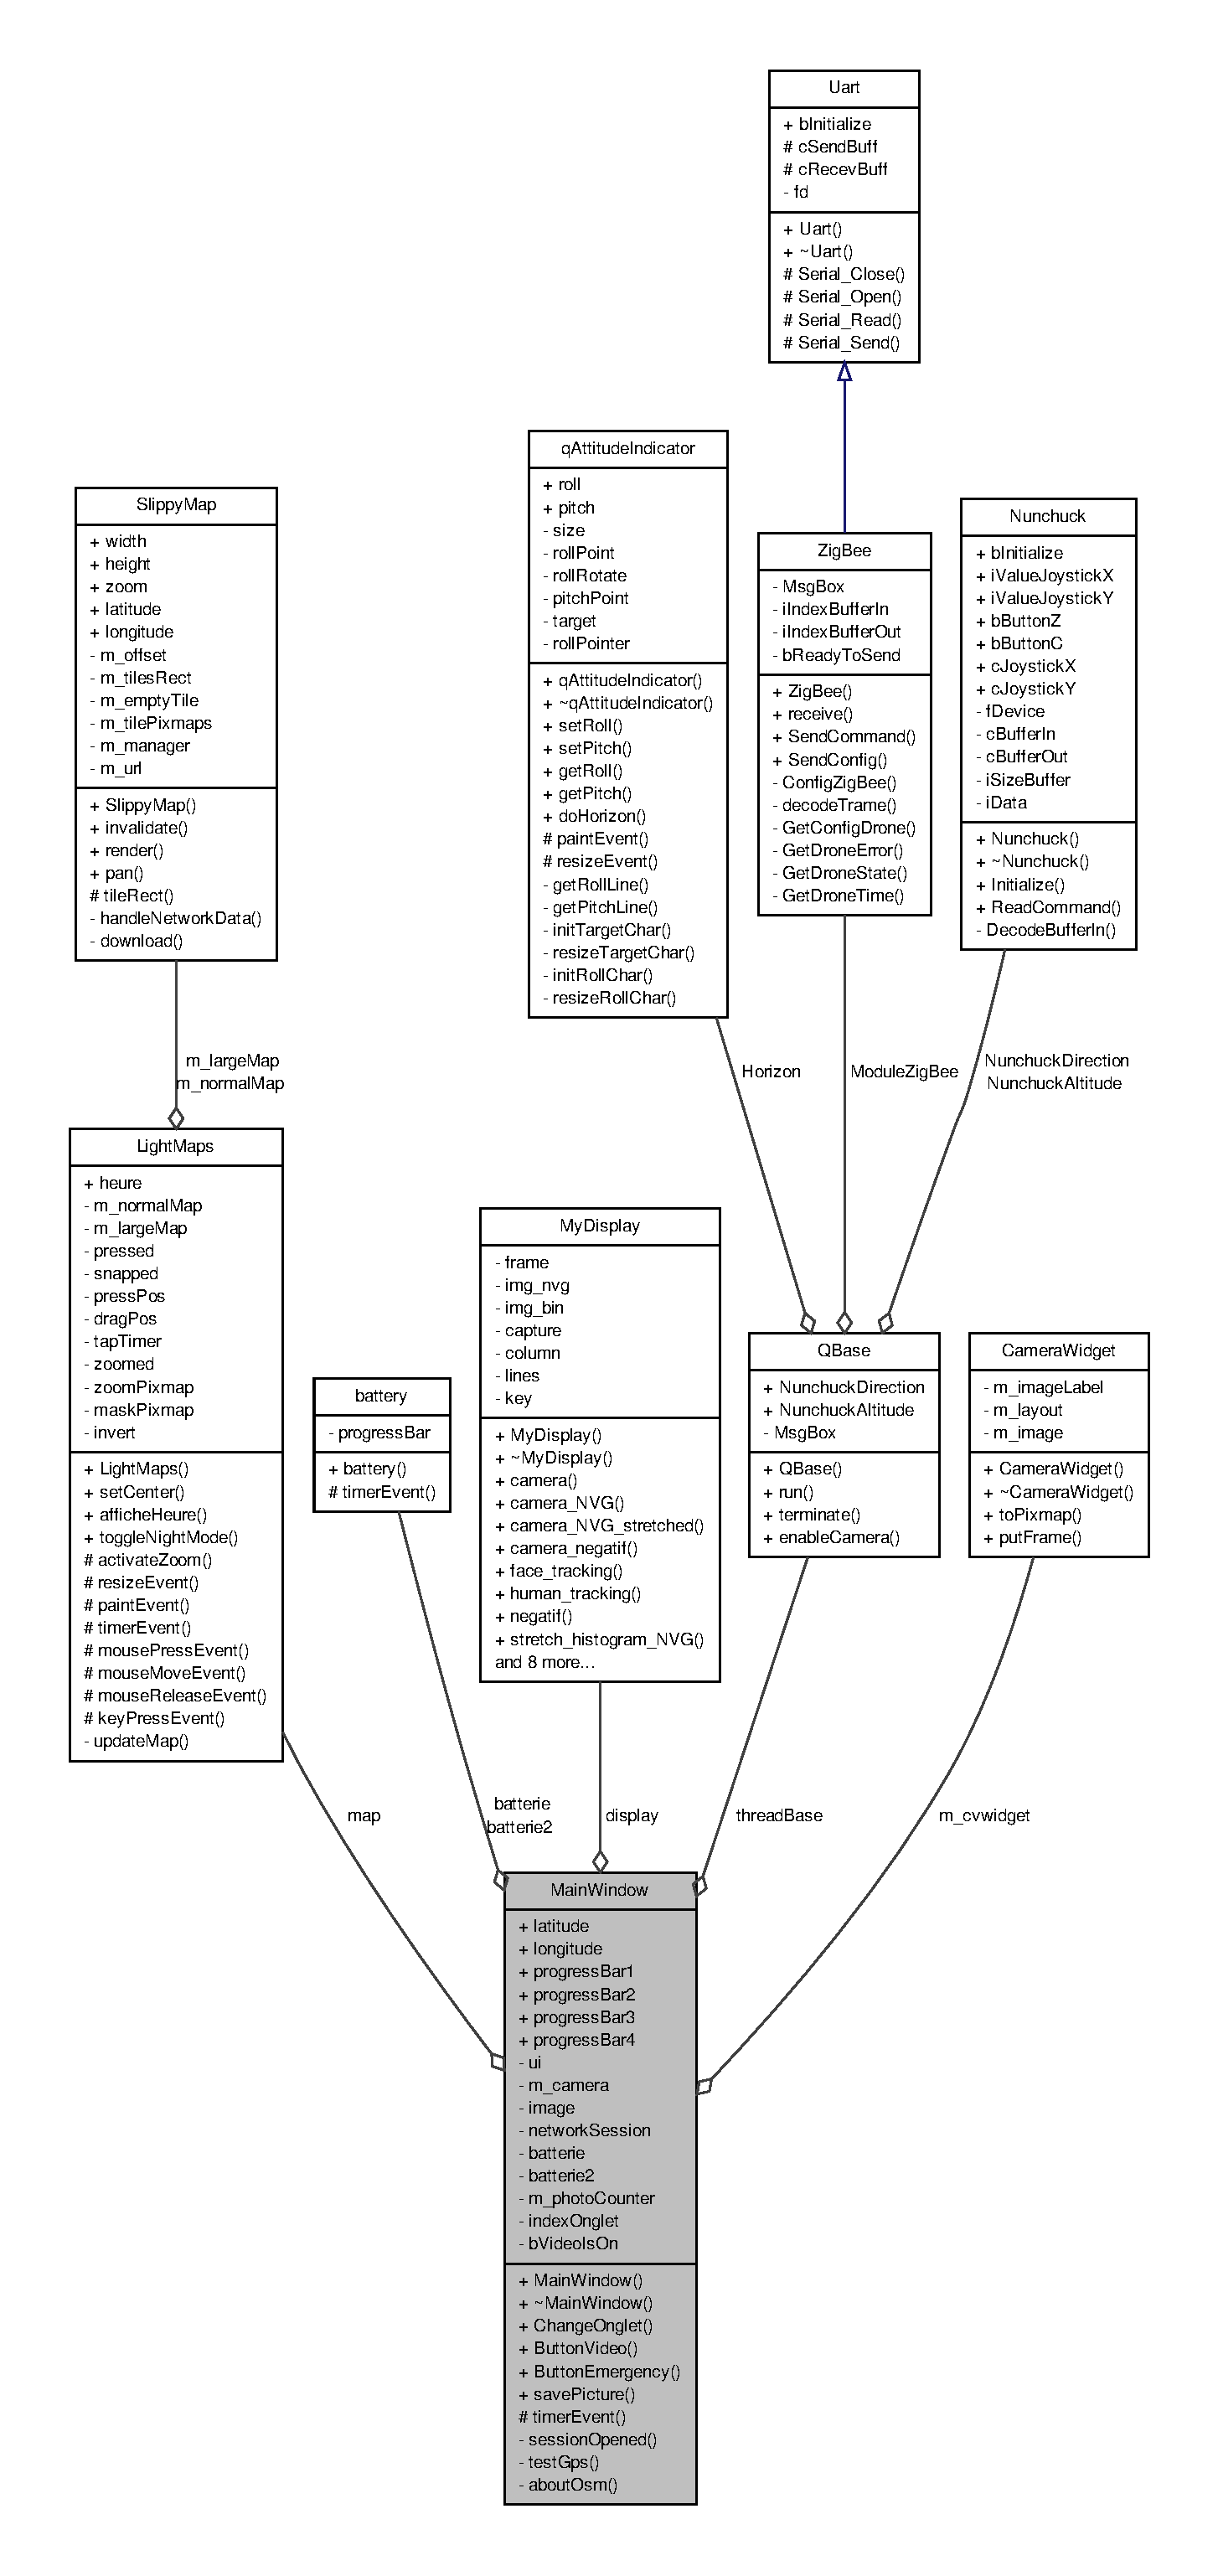
\includegraphics[height=550pt]{classMainWindow__coll__graph}
\end{center}
\end{figure}
\subsection*{Public Slots}
\begin{DoxyCompactItemize}
\item 
void \hyperlink{classMainWindow_a613b559650b3fe5dbe121de8abe92917}{Change\-Onglet} (int index)
\begin{DoxyCompactList}\small\item\em Changement d'onglet. \end{DoxyCompactList}\item 
void \hyperlink{classMainWindow_ad4e4c739790c121e308e876b490f6da9}{Button\-Video} ()
\begin{DoxyCompactList}\small\item\em Button\-Video. \end{DoxyCompactList}\item 
void \hyperlink{classMainWindow_a5d732a8b1e964a00dd04ed8ec2f5c1ef}{Button\-Emergency} ()
\begin{DoxyCompactList}\small\item\em Arrêt d'urgence. \end{DoxyCompactList}\item 
void \hyperlink{classMainWindow_a4d4b2c73d974fd4dbce801bdaf9b71f2}{save\-Picture} (void)
\begin{DoxyCompactList}\small\item\em Prise de photos. \end{DoxyCompactList}\end{DoxyCompactItemize}
\subsection*{Public Member Functions}
\begin{DoxyCompactItemize}
\item 
\hyperlink{classMainWindow_a8b244be8b7b7db1b08de2a2acb9409db}{Main\-Window} (Q\-Widget $\ast$parent=0)
\begin{DoxyCompactList}\small\item\em Constructeur. \end{DoxyCompactList}\item 
\hyperlink{classMainWindow_ae98d00a93bc118200eeef9f9bba1dba7}{$\sim$\-Main\-Window} ()
\begin{DoxyCompactList}\small\item\em Destructeur. \end{DoxyCompactList}\end{DoxyCompactItemize}
\subsection*{Public Attributes}
\begin{DoxyCompactItemize}
\item 
qreal \hyperlink{classMainWindow_a8eb6f9adebecfb3cf78c566686f1f35e}{latitude}
\item 
qreal \hyperlink{classMainWindow_ac7c0f22da72ad33678ff3d3e22c722c7}{longitude}
\item 
Q\-Progress\-Bar $\ast$ \hyperlink{classMainWindow_a50d8f5aa716821eca4ad0a3bfb0cf2ec}{progress\-Bar1}
\item 
Q\-Progress\-Bar $\ast$ \hyperlink{classMainWindow_a0594f2275ce1af436549e95cf62cfe7d}{progress\-Bar2}
\item 
Q\-Progress\-Bar $\ast$ \hyperlink{classMainWindow_a4afea90f9ba8cd1d26fa3b552639a012}{progress\-Bar3}
\item 
Q\-Progress\-Bar $\ast$ \hyperlink{classMainWindow_a8672c729ad5494d2890676bf07518ea2}{progress\-Bar4}
\end{DoxyCompactItemize}
\subsection*{Protected Member Functions}
\begin{DoxyCompactItemize}
\item 
void \hyperlink{classMainWindow_a1c7877c1ca466bd8034d88762ce2af9f}{timer\-Event} (Q\-Timer\-Event $\ast$)
\begin{DoxyCompactList}\small\item\em Timer. \end{DoxyCompactList}\end{DoxyCompactItemize}
\subsection*{Private Slots}
\begin{DoxyCompactItemize}
\item 
void \hyperlink{classMainWindow_ab218243366728139f7af5b3d6d97e8af}{session\-Opened} ()
\item 
void \hyperlink{classMainWindow_a99e264f214b0841cb0f990ae7b103289}{test\-Gps} ()
\item 
void \hyperlink{classMainWindow_af8ce1443f9a63d9edb6207f6361c0b9c}{about\-Osm} ()
\end{DoxyCompactItemize}
\subsection*{Private Attributes}
\begin{DoxyCompactItemize}
\item 
Ui\-::\-Main\-Window $\ast$ \hyperlink{classMainWindow_a35466a70ed47252a0191168126a352a5}{ui}
\item 
\hyperlink{classQBase}{Q\-Base} $\ast$ \hyperlink{classMainWindow_aa35075e5c401c08057511b93444701cf}{thread\-Base}
\item 
\hyperlink{classCameraWidget}{Camera\-Widget} $\ast$ \hyperlink{classMainWindow_a3225ace47a46792151d14646b6429712}{m\-\_\-cvwidget}
\item 
Cv\-Capture $\ast$ \hyperlink{classMainWindow_a1e4ee7611df9ee764de50cd2bfdebc55}{m\-\_\-camera}
\item 
Ipl\-Image $\ast$ \hyperlink{classMainWindow_aeb45155a2035daf28097e853724529a1}{image}
\item 
\hyperlink{classMyDisplay}{My\-Display} \hyperlink{classMainWindow_a144a0c272b675a9e8721ee486d629874}{display}
\item 
\hyperlink{classLightMaps}{Light\-Maps} $\ast$ \hyperlink{classMainWindow_a2f9e7ca90c2813bd1969055871782cfb}{map}
\item 
Q\-Network\-Session $\ast$ \hyperlink{classMainWindow_a638a10aec0de799787205387ee4da83e}{network\-Session}
\item 
\hyperlink{classbattery}{battery} $\ast$ \hyperlink{classMainWindow_af02a0259f044a5b2a1feabffccbc227e}{batterie}
\item 
\hyperlink{classbattery}{battery} $\ast$ \hyperlink{classMainWindow_a2c5aa6244af6d3e2018b98f285b0b84a}{batterie2}
\item 
int \hyperlink{classMainWindow_a264802533d4b55dce30d220ba9559471}{m\-\_\-photo\-Counter}
\item 
int \hyperlink{classMainWindow_a2cf797221c17fdcce7888b123bd5847b}{index\-Onglet}
\item 
bool \hyperlink{classMainWindow_a8f36c27c20d39c3f0eafe091b9f2cf29}{b\-Video\-Is\-On}
\end{DoxyCompactItemize}


\subsection{Detailed Description}


Definition at line 40 of file mainwindow.\-h.



\subsection{Constructor \& Destructor Documentation}
\hypertarget{classMainWindow_a8b244be8b7b7db1b08de2a2acb9409db}{\index{Main\-Window@{Main\-Window}!Main\-Window@{Main\-Window}}
\index{Main\-Window@{Main\-Window}!MainWindow@{Main\-Window}}
\subsubsection[{Main\-Window}]{\setlength{\rightskip}{0pt plus 5cm}Main\-Window\-::\-Main\-Window (
\begin{DoxyParamCaption}
\item[{Q\-Widget $\ast$}]{parent = {\ttfamily 0}}
\end{DoxyParamCaption}
)\hspace{0.3cm}{\ttfamily [explicit]}}}\label{classMainWindow_a8b244be8b7b7db1b08de2a2acb9409db}


Constructeur. 

Permet la déclaration des widgets présents dans l'application. 
\begin{DoxyParams}{Parameters}
{\em Q\-Widget} & $\ast$parent \\
\hline
\end{DoxyParams}


Definition at line 47 of file mainwindow.\-cpp.



References about\-Osm(), batterie, batterie2, Button\-Video(), b\-Video\-Is\-On, Change\-Onglet(), index\-Onglet, m\-\_\-cvwidget, m\-\_\-photo\-Counter, map, network\-Session, progress\-Bar1, progress\-Bar2, progress\-Bar3, progress\-Bar4, save\-Picture(), session\-Opened(), test\-Gps(), thread\-Base, and ui.


\begin{DoxyCode}
                                      :
    QMainWindow(parent),
    \hyperlink{classMainWindow_a35466a70ed47252a0191168126a352a5}{ui}(\textcolor{keyword}{new} Ui::MainWindow)
\{
    \hyperlink{classMainWindow_a35466a70ed47252a0191168126a352a5}{ui}->setupUi(\textcolor{keyword}{this});

    \textcolor{comment}{/* Déclaration du widget permettant l'affichage vidéo des et du thread
       utilisé pour la communication et l'affichange de l'horizon artificiel */}

    \hyperlink{classMainWindow_aa35075e5c401c08057511b93444701cf}{threadBase} = \textcolor{keyword}{new} \hyperlink{classQBase}{QBase}();
    \hyperlink{classMainWindow_a3225ace47a46792151d14646b6429712}{m\_cvwidget} = \textcolor{keyword}{new} \hyperlink{classCameraWidget}{CameraWidget}();

    \textcolor{comment}{/* Déclaration du widget permettant l'affichage de l'état de la batterie et
       placement dans les layouts définis à l'aide de QtDesigner */}

    \hyperlink{classMainWindow_af02a0259f044a5b2a1feabffccbc227e}{batterie} = \textcolor{keyword}{new} \hyperlink{classbattery}{battery};
    \hyperlink{classMainWindow_a35466a70ed47252a0191168126a352a5}{ui}->batterylayout->addWidget(\hyperlink{classMainWindow_af02a0259f044a5b2a1feabffccbc227e}{batterie});
    \hyperlink{classMainWindow_a2c5aa6244af6d3e2018b98f285b0b84a}{batterie2} = \textcolor{keyword}{new} \hyperlink{classbattery}{battery};
    \hyperlink{classMainWindow_a35466a70ed47252a0191168126a352a5}{ui}->batterylayout\_2->addWidget(\hyperlink{classMainWindow_a2c5aa6244af6d3e2018b98f285b0b84a}{batterie2});

    \textcolor{comment}{/* Déclaration des progressBars permettant l'affichage de la puissance du
       signal */}

    \hyperlink{classMainWindow_a50d8f5aa716821eca4ad0a3bfb0cf2ec}{progressBar1} = \textcolor{keyword}{new} QProgressBar(\textcolor{keyword}{this});
    \hyperlink{classMainWindow_a50d8f5aa716821eca4ad0a3bfb0cf2ec}{progressBar1}->setGeometry(10, 10, 5, 10);
    \hyperlink{classMainWindow_a50d8f5aa716821eca4ad0a3bfb0cf2ec}{progressBar1}->setOrientation(Qt::Vertical);
    \hyperlink{classMainWindow_a50d8f5aa716821eca4ad0a3bfb0cf2ec}{progressBar1}->setTextVisible(\textcolor{keyword}{false});
    \hyperlink{classMainWindow_a50d8f5aa716821eca4ad0a3bfb0cf2ec}{progressBar1}->setStyleSheet(\textcolor{stringliteral}{"
      QProgressBar::chunk\{background-color:orange\}"});
    \hyperlink{classMainWindow_a0594f2275ce1af436549e95cf62cfe7d}{progressBar2} = \textcolor{keyword}{new} QProgressBar(\textcolor{keyword}{this});
    \hyperlink{classMainWindow_a0594f2275ce1af436549e95cf62cfe7d}{progressBar2}->setGeometry(10, 10, 5, 20);
    \hyperlink{classMainWindow_a0594f2275ce1af436549e95cf62cfe7d}{progressBar2}->setOrientation(Qt::Vertical);
    \hyperlink{classMainWindow_a0594f2275ce1af436549e95cf62cfe7d}{progressBar2}->setTextVisible(\textcolor{keyword}{false});
    \hyperlink{classMainWindow_a0594f2275ce1af436549e95cf62cfe7d}{progressBar2}->setStyleSheet(\textcolor{stringliteral}{"
      QProgressBar::chunk\{background-color:orange\}"});
    \hyperlink{classMainWindow_a4afea90f9ba8cd1d26fa3b552639a012}{progressBar3} = \textcolor{keyword}{new} QProgressBar(\textcolor{keyword}{this});
    \hyperlink{classMainWindow_a4afea90f9ba8cd1d26fa3b552639a012}{progressBar3}->setGeometry(10, 10, 5, 30);
    \hyperlink{classMainWindow_a4afea90f9ba8cd1d26fa3b552639a012}{progressBar3}->setOrientation(Qt::Vertical);
    \hyperlink{classMainWindow_a4afea90f9ba8cd1d26fa3b552639a012}{progressBar3}->setTextVisible(\textcolor{keyword}{false});
    \hyperlink{classMainWindow_a4afea90f9ba8cd1d26fa3b552639a012}{progressBar3}->setStyleSheet(\textcolor{stringliteral}{"
      QProgressBar::chunk\{background-color:orange\}"});
    \hyperlink{classMainWindow_a8672c729ad5494d2890676bf07518ea2}{progressBar4} = \textcolor{keyword}{new} QProgressBar(\textcolor{keyword}{this});
    \hyperlink{classMainWindow_a8672c729ad5494d2890676bf07518ea2}{progressBar4}->setGeometry(10, 10, 5, 40);
    \hyperlink{classMainWindow_a8672c729ad5494d2890676bf07518ea2}{progressBar4}->setOrientation(Qt::Vertical);
    \hyperlink{classMainWindow_a8672c729ad5494d2890676bf07518ea2}{progressBar4}->setTextVisible(\textcolor{keyword}{false});
    \hyperlink{classMainWindow_a8672c729ad5494d2890676bf07518ea2}{progressBar4}->setStyleSheet(\textcolor{stringliteral}{"
      QProgressBar::chunk\{background-color:orange\}"});

    \textcolor{comment}{//startTimer(200);}

    \textcolor{comment}{/* Ajout des widgets affichant la puissance du signal dans les layouts
       prédéfinis à l'aide de QtDesigner */}

    \hyperlink{classMainWindow_a35466a70ed47252a0191168126a352a5}{ui}->powerlayout1->addWidget(\hyperlink{classMainWindow_a50d8f5aa716821eca4ad0a3bfb0cf2ec}{progressBar1});
    \hyperlink{classMainWindow_a35466a70ed47252a0191168126a352a5}{ui}->powerlayout2->addWidget(\hyperlink{classMainWindow_a0594f2275ce1af436549e95cf62cfe7d}{progressBar2});
    \hyperlink{classMainWindow_a35466a70ed47252a0191168126a352a5}{ui}->powerlayout3->addWidget(\hyperlink{classMainWindow_a4afea90f9ba8cd1d26fa3b552639a012}{progressBar3});
    \hyperlink{classMainWindow_a35466a70ed47252a0191168126a352a5}{ui}->powerlayout4->addWidget(\hyperlink{classMainWindow_a8672c729ad5494d2890676bf07518ea2}{progressBar4});



    \textcolor{comment}{/* Déclaration du widget Lightmaps afin d'afficher la carte dans un layout
       préfdéfini à l'aide de QtDesigner */}

    \hyperlink{classMainWindow_a2f9e7ca90c2813bd1969055871782cfb}{map} = \textcolor{keyword}{new} \hyperlink{classLightMaps}{LightMaps}();
    \hyperlink{classMainWindow_a35466a70ed47252a0191168126a352a5}{ui}->maplayout->addWidget(\hyperlink{classMainWindow_a2f9e7ca90c2813bd1969055871782cfb}{map});
    \hyperlink{classMainWindow_a2f9e7ca90c2813bd1969055871782cfb}{map}->setFocus();

    \textcolor{comment}{/*m\_normalMap = new SlippyMap(this);}
\textcolor{comment}{    connect(m\_normalMap, SIGNAL(updated(QRect)), SLOT(updateMap(QRect)));*/}

    QAction *testGpsAction = \textcolor{keyword}{new} QAction(tr(\textcolor{stringliteral}{"&testGps"}), \textcolor{keyword}{this});
    QAction *nightModeAction = \textcolor{keyword}{new} QAction(tr(\textcolor{stringliteral}{"Night Mode"}), \textcolor{keyword}{this});
    nightModeAction->setCheckable(\textcolor{keyword}{true});
    nightModeAction->setChecked(\textcolor{keyword}{false});
    QAction *osmAction = \textcolor{keyword}{new} QAction(tr(\textcolor{stringliteral}{"About OpenStreetMap"}), \textcolor{keyword}{this});
    connect(testGpsAction, SIGNAL(triggered()), SLOT(\hyperlink{classMainWindow_a99e264f214b0841cb0f990ae7b103289}{testGps}()));
    connect(nightModeAction, SIGNAL(triggered()), \hyperlink{classMainWindow_a2f9e7ca90c2813bd1969055871782cfb}{map}, SLOT(toggleNightMode(
      )));
    connect(osmAction, SIGNAL(triggered()), SLOT(\hyperlink{classMainWindow_af8ce1443f9a63d9edb6207f6361c0b9c}{aboutOsm}()));

\textcolor{preprocessor}{    #if defined(Q\_OS\_SYMBIAN) || defined(Q\_OS\_WINCE\_WM)}
\textcolor{preprocessor}{}        menuBar()->addAction(testGpsAction);
        menuBar()->addAction(nightModeAction);
        menuBar()->addAction(osmAction);
\textcolor{preprocessor}{    #else}
\textcolor{preprocessor}{}        QMenu *menu = menuBar()->addMenu(tr(\textcolor{stringliteral}{"&Options"}));
        menu->addAction(testGpsAction);
        menu->addSeparator();
        menu->addAction(nightModeAction);
        menu->addAction(osmAction);
\textcolor{preprocessor}{    #endif}
\textcolor{preprocessor}{}
    QNetworkConfigurationManager manager;
    \textcolor{keywordflow}{if} (manager.capabilities() & 
      QNetworkConfigurationManager::NetworkSessionRequired)
    \{
            \textcolor{comment}{// Get saved network configuration}
            QSettings settings(QSettings::UserScope, QLatin1String(\textcolor{stringliteral}{"Trolltech"})
      );
            settings.beginGroup(QLatin1String(\textcolor{stringliteral}{"QtNetwork"}));
            \textcolor{keyword}{const} QString \textcolor{keywordtype}{id} =
                settings.value(QLatin1String(\textcolor{stringliteral}{"DefaultNetworkConfiguration"})).
      toString();
            settings.endGroup();

            \textcolor{comment}{// If the saved network configuration is not currently discovered
       use the system}
            \textcolor{comment}{// default}
            QNetworkConfiguration config = manager.configurationFromIdentifier(\textcolor{keywordtype}{
      id});
            \textcolor{keywordflow}{if} ((config.state() & QNetworkConfiguration::Discovered) !=
                QNetworkConfiguration::Discovered)
            \{
                config = manager.defaultConfiguration();
            \}

            \hyperlink{classMainWindow_a638a10aec0de799787205387ee4da83e}{networkSession} = \textcolor{keyword}{new} QNetworkSession(config, \textcolor{keyword}{this});
            connect(\hyperlink{classMainWindow_a638a10aec0de799787205387ee4da83e}{networkSession}, SIGNAL(opened()), \textcolor{keyword}{this}, SLOT(
      \hyperlink{classMainWindow_ab218243366728139f7af5b3d6d97e8af}{sessionOpened}()));

            \hyperlink{classMainWindow_a638a10aec0de799787205387ee4da83e}{networkSession}->open();
    \}

    \textcolor{keywordflow}{else}
    \{
            \hyperlink{classMainWindow_a638a10aec0de799787205387ee4da83e}{networkSession} = 0;
    \}

    \textcolor{comment}{/* Ajout d'un titre pour l'application */}

    setWindowTitle(tr(\textcolor{stringliteral}{"WELCOME TO THE APPLICATION OF ESTEI STUDENTS !"}));
    \textcolor{comment}{//startTimer(200);}


    \hyperlink{classMainWindow_a2cf797221c17fdcce7888b123bd5847b}{indexOnglet} = \hyperlink{classMainWindow_a35466a70ed47252a0191168126a352a5}{ui}->Onglet->currentIndex();
    \hyperlink{classMainWindow_a8f36c27c20d39c3f0eafe091b9f2cf29}{bVideoIsOn} = \textcolor{keyword}{false};

    \textcolor{comment}{/* Mise à zéro de m\_photoCounter et connexion entre le bouton "SAVE
       PICTURE" et la fonction décrite plus bas dans ce fichier */}

    \hyperlink{classMainWindow_a264802533d4b55dce30d220ba9559471}{m\_photoCounter} = 0;
    connect(\hyperlink{classMainWindow_a35466a70ed47252a0191168126a352a5}{ui}->Photo, SIGNAL(pressed()), \textcolor{keyword}{this}, SLOT(\hyperlink{classMainWindow_a4d4b2c73d974fd4dbce801bdaf9b71f2}{savePicture}()
      ));

    \textcolor{comment}{/* Connexion du bouton "START/STOP VIDEO STREAMING" au slot ButtonVideo */}

    connect(\hyperlink{classMainWindow_a35466a70ed47252a0191168126a352a5}{ui}->Onglet, SIGNAL(currentChanged(\textcolor{keywordtype}{int})), \textcolor{keyword}{this}, SLOT(\hyperlink{classMainWindow_a613b559650b3fe5dbe121de8abe92917}{ChangeOnglet}
      (\textcolor{keywordtype}{int})));
    connect(\hyperlink{classMainWindow_a35466a70ed47252a0191168126a352a5}{ui}->VideoStreaming, SIGNAL(clicked()), \textcolor{keyword}{this}, SLOT(\hyperlink{classMainWindow_ad4e4c739790c121e308e876b490f6da9}{ButtonVideo}
      ()));
    startTimer(47);     \textcolor{comment}{/* Environ 21 images/s */}

    \textcolor{comment}{/*  Lancement du thread */}
    \hyperlink{classMainWindow_aa35075e5c401c08057511b93444701cf}{threadBase}->start();

\}
\end{DoxyCode}
\hypertarget{classMainWindow_ae98d00a93bc118200eeef9f9bba1dba7}{\index{Main\-Window@{Main\-Window}!$\sim$\-Main\-Window@{$\sim$\-Main\-Window}}
\index{$\sim$\-Main\-Window@{$\sim$\-Main\-Window}!MainWindow@{Main\-Window}}
\subsubsection[{$\sim$\-Main\-Window}]{\setlength{\rightskip}{0pt plus 5cm}Main\-Window\-::$\sim$\-Main\-Window (
\begin{DoxyParamCaption}
{}
\end{DoxyParamCaption}
)}}\label{classMainWindow_ae98d00a93bc118200eeef9f9bba1dba7}


Destructeur. 

Permet la destruction du thread et de la capture vidéo. 
\begin{DoxyParams}{Parameters}
{\em void} & \\
\hline
\end{DoxyParams}


Definition at line 190 of file mainwindow.\-cpp.



References m\-\_\-camera, thread\-Base, and ui.


\begin{DoxyCode}
\{
    \textcolor{keywordflow}{if}(\hyperlink{classMainWindow_a1e4ee7611df9ee764de50cd2bfdebc55}{m\_camera} != NULL)                                               
               \textcolor{comment}{/* Appel à la fonction qui permet de détruire la capture de la vidéo si
       son argument n'est pas nul */}
        cvReleaseCapture(&\hyperlink{classMainWindow_a1e4ee7611df9ee764de50cd2bfdebc55}{m\_camera});
    \hyperlink{classMainWindow_aa35075e5c401c08057511b93444701cf}{threadBase}->deleteLater();                                       
                 \textcolor{comment}{/* Destruction du thread */}
    \textcolor{keyword}{delete} \hyperlink{classMainWindow_a35466a70ed47252a0191168126a352a5}{ui};                                                               
         \textcolor{comment}{/* Destruction du fichier .ui */}
\}
\end{DoxyCode}


\subsection{Member Function Documentation}
\hypertarget{classMainWindow_af8ce1443f9a63d9edb6207f6361c0b9c}{\index{Main\-Window@{Main\-Window}!about\-Osm@{about\-Osm}}
\index{about\-Osm@{about\-Osm}!MainWindow@{Main\-Window}}
\subsubsection[{about\-Osm}]{\setlength{\rightskip}{0pt plus 5cm}void Main\-Window\-::about\-Osm (
\begin{DoxyParamCaption}
{}
\end{DoxyParamCaption}
)\hspace{0.3cm}{\ttfamily [private]}, {\ttfamily [slot]}}}\label{classMainWindow_af8ce1443f9a63d9edb6207f6361c0b9c}


Definition at line 250 of file mainwindow.\-cpp.



Referenced by Main\-Window().


\begin{DoxyCode}
\{
    QDesktopServices::openUrl(QUrl(\textcolor{stringliteral}{"http://www.openstreetmap.org"}));
\}
\end{DoxyCode}
\hypertarget{classMainWindow_a5d732a8b1e964a00dd04ed8ec2f5c1ef}{\index{Main\-Window@{Main\-Window}!Button\-Emergency@{Button\-Emergency}}
\index{Button\-Emergency@{Button\-Emergency}!MainWindow@{Main\-Window}}
\subsubsection[{Button\-Emergency}]{\setlength{\rightskip}{0pt plus 5cm}void Main\-Window\-::\-Button\-Emergency (
\begin{DoxyParamCaption}
{}
\end{DoxyParamCaption}
)\hspace{0.3cm}{\ttfamily [slot]}}}\label{classMainWindow_a5d732a8b1e964a00dd04ed8ec2f5c1ef}


Arrêt d'urgence. 

Permet l'arrêt du drône en cas de grave problème. 
\begin{DoxyParams}{Parameters}
{\em void} & \\
\hline
\end{DoxyParams}


Definition at line 461 of file mainwindow.\-cpp.


\begin{DoxyCode}
\{

\}
\end{DoxyCode}
\hypertarget{classMainWindow_ad4e4c739790c121e308e876b490f6da9}{\index{Main\-Window@{Main\-Window}!Button\-Video@{Button\-Video}}
\index{Button\-Video@{Button\-Video}!MainWindow@{Main\-Window}}
\subsubsection[{Button\-Video}]{\setlength{\rightskip}{0pt plus 5cm}void Main\-Window\-::\-Button\-Video (
\begin{DoxyParamCaption}
{}
\end{DoxyParamCaption}
)\hspace{0.3cm}{\ttfamily [slot]}}}\label{classMainWindow_ad4e4c739790c121e308e876b490f6da9}


Button\-Video. 

Fonction permettant la destructution ou l'ajout du widget permettant la capture de la vidéo. 
\begin{DoxyParams}{Parameters}
{\em void} & \\
\hline
\end{DoxyParams}


Definition at line 438 of file mainwindow.\-cpp.



References b\-Video\-Is\-On, m\-\_\-camera, m\-\_\-cvwidget, and ui.



Referenced by Main\-Window().


\begin{DoxyCode}
\{
    \textcolor{keywordflow}{if}(\hyperlink{classMainWindow_a8f36c27c20d39c3f0eafe091b9f2cf29}{bVideoIsOn})
    \{
        \hyperlink{classMainWindow_a35466a70ed47252a0191168126a352a5}{ui}->cameralayout->removeWidget(\hyperlink{classMainWindow_a3225ace47a46792151d14646b6429712}{m\_cvwidget});
        cvReleaseCapture(&\hyperlink{classMainWindow_a1e4ee7611df9ee764de50cd2bfdebc55}{m\_camera});
        \hyperlink{classMainWindow_a8f36c27c20d39c3f0eafe091b9f2cf29}{bVideoIsOn} = \textcolor{keyword}{false};
    \}

    \textcolor{keywordflow}{else}
    \{
        \hyperlink{classMainWindow_a35466a70ed47252a0191168126a352a5}{ui}->cameralayout->addWidget(\hyperlink{classMainWindow_a3225ace47a46792151d14646b6429712}{m\_cvwidget});
        \hyperlink{classMainWindow_a1e4ee7611df9ee764de50cd2bfdebc55}{m\_camera} = cvCreateCameraCapture(0);
        \hyperlink{classMainWindow_a8f36c27c20d39c3f0eafe091b9f2cf29}{bVideoIsOn} = \textcolor{keyword}{true};
    \}
\}
\end{DoxyCode}
\hypertarget{classMainWindow_a613b559650b3fe5dbe121de8abe92917}{\index{Main\-Window@{Main\-Window}!Change\-Onglet@{Change\-Onglet}}
\index{Change\-Onglet@{Change\-Onglet}!MainWindow@{Main\-Window}}
\subsubsection[{Change\-Onglet}]{\setlength{\rightskip}{0pt plus 5cm}void Main\-Window\-::\-Change\-Onglet (
\begin{DoxyParamCaption}
\item[{int}]{index}
\end{DoxyParamCaption}
)\hspace{0.3cm}{\ttfamily [slot]}}}\label{classMainWindow_a613b559650b3fe5dbe121de8abe92917}


Changement d'onglet. 

Fonction qui permet l'ajout ou la destruction de widgets suivant l'onglet sélectionnée. 
\begin{DoxyParams}{Parameters}
{\em int} & index \\
\hline
\end{DoxyParams}


Definition at line 383 of file mainwindow.\-cpp.



References batterie, batterie2, Q\-Base\-::\-Horizon, I\-N\-D\-E\-X\-\_\-\-O\-N\-G\-L\-E\-T\-\_\-\-C\-A\-M\-E\-R\-A, I\-N\-D\-E\-X\-\_\-\-O\-N\-G\-L\-E\-T\-\_\-\-H\-O\-R\-I\-Z\-O\-N, index\-Onglet, map, progress\-Bar1, progress\-Bar2, progress\-Bar3, progress\-Bar4, thread\-Base, and ui.



Referenced by Main\-Window().


\begin{DoxyCode}
\{
    \hyperlink{classMainWindow_a2cf797221c17fdcce7888b123bd5847b}{indexOnglet} = index;

    \textcolor{keywordflow}{switch}(\hyperlink{classMainWindow_a2cf797221c17fdcce7888b123bd5847b}{indexOnglet}) \{

    \textcolor{keywordflow}{case} \hyperlink{mainwindow_8h_ab9f3d4f131379475d4b36a15d2b59b5e}{INDEX\_ONGLET\_CAMERA}:
            \hyperlink{classMainWindow_a35466a70ed47252a0191168126a352a5}{ui}->horizon\_layout->removeWidget(\hyperlink{classMainWindow_aa35075e5c401c08057511b93444701cf}{threadBase}->\hyperlink{classQBase_ae4a8b78621695d9a61c311d422824a8d}{Horizon}
      );
            \hyperlink{classMainWindow_a35466a70ed47252a0191168126a352a5}{ui}->maplayout2->removeWidget(\hyperlink{classMainWindow_a2f9e7ca90c2813bd1969055871782cfb}{map});
            \hyperlink{classMainWindow_a35466a70ed47252a0191168126a352a5}{ui}->maplayout->addWidget(\hyperlink{classMainWindow_a2f9e7ca90c2813bd1969055871782cfb}{map});
            \hyperlink{classMainWindow_a35466a70ed47252a0191168126a352a5}{ui}->batterylayout2->removeWidget(\hyperlink{classMainWindow_af02a0259f044a5b2a1feabffccbc227e}{batterie});
            \hyperlink{classMainWindow_a35466a70ed47252a0191168126a352a5}{ui}->batterylayout->addWidget(\hyperlink{classMainWindow_af02a0259f044a5b2a1feabffccbc227e}{batterie});
            \hyperlink{classMainWindow_a35466a70ed47252a0191168126a352a5}{ui}->batterylayout2\_2->removeWidget(\hyperlink{classMainWindow_a2c5aa6244af6d3e2018b98f285b0b84a}{batterie2});
            \hyperlink{classMainWindow_a35466a70ed47252a0191168126a352a5}{ui}->batterylayout\_2->addWidget(\hyperlink{classMainWindow_a2c5aa6244af6d3e2018b98f285b0b84a}{batterie2});
            \hyperlink{classMainWindow_a35466a70ed47252a0191168126a352a5}{ui}->powerlayout1\_2->removeWidget(\hyperlink{classMainWindow_a50d8f5aa716821eca4ad0a3bfb0cf2ec}{progressBar1});
            \hyperlink{classMainWindow_a35466a70ed47252a0191168126a352a5}{ui}->powerlayout2\_2->removeWidget(\hyperlink{classMainWindow_a0594f2275ce1af436549e95cf62cfe7d}{progressBar2});
            \hyperlink{classMainWindow_a35466a70ed47252a0191168126a352a5}{ui}->powerlayout3\_2->removeWidget(\hyperlink{classMainWindow_a4afea90f9ba8cd1d26fa3b552639a012}{progressBar3});
            \hyperlink{classMainWindow_a35466a70ed47252a0191168126a352a5}{ui}->powerlayout4\_2->removeWidget(\hyperlink{classMainWindow_a8672c729ad5494d2890676bf07518ea2}{progressBar4});
            \hyperlink{classMainWindow_a35466a70ed47252a0191168126a352a5}{ui}->powerlayout1->addWidget(\hyperlink{classMainWindow_a50d8f5aa716821eca4ad0a3bfb0cf2ec}{progressBar1});
            \hyperlink{classMainWindow_a35466a70ed47252a0191168126a352a5}{ui}->powerlayout2->addWidget(\hyperlink{classMainWindow_a0594f2275ce1af436549e95cf62cfe7d}{progressBar2});
            \hyperlink{classMainWindow_a35466a70ed47252a0191168126a352a5}{ui}->powerlayout3->addWidget(\hyperlink{classMainWindow_a4afea90f9ba8cd1d26fa3b552639a012}{progressBar3});
            \hyperlink{classMainWindow_a35466a70ed47252a0191168126a352a5}{ui}->powerlayout4->addWidget(\hyperlink{classMainWindow_a8672c729ad5494d2890676bf07518ea2}{progressBar4});

        \textcolor{keywordflow}{break};

    \textcolor{keywordflow}{case} \hyperlink{mainwindow_8h_ac416243e121530c2fc222e5204d7fe30}{INDEX\_ONGLET\_HORIZON}:
            \hyperlink{classMainWindow_a35466a70ed47252a0191168126a352a5}{ui}->horizon\_layout->addWidget(\hyperlink{classMainWindow_aa35075e5c401c08057511b93444701cf}{threadBase}->\hyperlink{classQBase_ae4a8b78621695d9a61c311d422824a8d}{Horizon}
      );
            \hyperlink{classMainWindow_a35466a70ed47252a0191168126a352a5}{ui}->maplayout->removeWidget(\hyperlink{classMainWindow_a2f9e7ca90c2813bd1969055871782cfb}{map});
            \hyperlink{classMainWindow_a35466a70ed47252a0191168126a352a5}{ui}->maplayout2->addWidget(\hyperlink{classMainWindow_a2f9e7ca90c2813bd1969055871782cfb}{map});
            \hyperlink{classMainWindow_a35466a70ed47252a0191168126a352a5}{ui}->batterylayout->removeWidget(\hyperlink{classMainWindow_af02a0259f044a5b2a1feabffccbc227e}{batterie});
            \hyperlink{classMainWindow_a35466a70ed47252a0191168126a352a5}{ui}->batterylayout2->addWidget(\hyperlink{classMainWindow_af02a0259f044a5b2a1feabffccbc227e}{batterie});
            \hyperlink{classMainWindow_a35466a70ed47252a0191168126a352a5}{ui}->batterylayout\_2->removeWidget(\hyperlink{classMainWindow_a2c5aa6244af6d3e2018b98f285b0b84a}{batterie2});
            \hyperlink{classMainWindow_a35466a70ed47252a0191168126a352a5}{ui}->batterylayout2\_2->addWidget(\hyperlink{classMainWindow_a2c5aa6244af6d3e2018b98f285b0b84a}{batterie2});
            \hyperlink{classMainWindow_a35466a70ed47252a0191168126a352a5}{ui}->powerlayout1->removeWidget(\hyperlink{classMainWindow_a50d8f5aa716821eca4ad0a3bfb0cf2ec}{progressBar1});
            \hyperlink{classMainWindow_a35466a70ed47252a0191168126a352a5}{ui}->powerlayout2->removeWidget(\hyperlink{classMainWindow_a0594f2275ce1af436549e95cf62cfe7d}{progressBar2});
            \hyperlink{classMainWindow_a35466a70ed47252a0191168126a352a5}{ui}->powerlayout3->removeWidget(\hyperlink{classMainWindow_a4afea90f9ba8cd1d26fa3b552639a012}{progressBar3});
            \hyperlink{classMainWindow_a35466a70ed47252a0191168126a352a5}{ui}->powerlayout4->removeWidget(\hyperlink{classMainWindow_a8672c729ad5494d2890676bf07518ea2}{progressBar4});
            \hyperlink{classMainWindow_a35466a70ed47252a0191168126a352a5}{ui}->powerlayout1\_2->addWidget(\hyperlink{classMainWindow_a50d8f5aa716821eca4ad0a3bfb0cf2ec}{progressBar1});
            \hyperlink{classMainWindow_a35466a70ed47252a0191168126a352a5}{ui}->powerlayout2\_2->addWidget(\hyperlink{classMainWindow_a0594f2275ce1af436549e95cf62cfe7d}{progressBar2});
            \hyperlink{classMainWindow_a35466a70ed47252a0191168126a352a5}{ui}->powerlayout3\_2->addWidget(\hyperlink{classMainWindow_a4afea90f9ba8cd1d26fa3b552639a012}{progressBar3});
            \hyperlink{classMainWindow_a35466a70ed47252a0191168126a352a5}{ui}->powerlayout4\_2->addWidget(\hyperlink{classMainWindow_a8672c729ad5494d2890676bf07518ea2}{progressBar4});

        \textcolor{keywordflow}{break};
    \textcolor{keywordflow}{default}:
        \textcolor{keywordflow}{break};
    \}
\}
\end{DoxyCode}
\hypertarget{classMainWindow_a4d4b2c73d974fd4dbce801bdaf9b71f2}{\index{Main\-Window@{Main\-Window}!save\-Picture@{save\-Picture}}
\index{save\-Picture@{save\-Picture}!MainWindow@{Main\-Window}}
\subsubsection[{save\-Picture}]{\setlength{\rightskip}{0pt plus 5cm}void Main\-Window\-::save\-Picture (
\begin{DoxyParamCaption}
\item[{void}]{}
\end{DoxyParamCaption}
)\hspace{0.3cm}{\ttfamily [slot]}}}\label{classMainWindow_a4d4b2c73d974fd4dbce801bdaf9b71f2}


Prise de photos. 

Fonction permettant l'enregistrement de photos via un appui sur le bouton \char`\"{}\-S\-A\-V\-E P\-I\-C\-T\-U\-R\-E\char`\"{}. 
\begin{DoxyParams}{Parameters}
{\em void} & \\
\hline
\end{DoxyParams}


Definition at line 472 of file mainwindow.\-cpp.



References image, m\-\_\-camera, m\-\_\-cvwidget, m\-\_\-photo\-Counter, and Camera\-Widget\-::to\-Pixmap().



Referenced by Main\-Window().


\begin{DoxyCode}
\{
    IplImage *\hyperlink{classMainWindow_aeb45155a2035daf28097e853724529a1}{image} = cvQueryFrame(\hyperlink{classMainWindow_a1e4ee7611df9ee764de50cd2bfdebc55}{m\_camera});
    QPixmap photo = \hyperlink{classMainWindow_a3225ace47a46792151d14646b6429712}{m\_cvwidget}->\hyperlink{classCameraWidget_a349b27ddfbcd67ae055f56e51ffe3e44}{toPixmap}(image);

    \textcolor{keywordflow}{if} (photo.save(\textcolor{stringliteral}{"/tmp/Picture"} + QString::number(\hyperlink{classMainWindow_a264802533d4b55dce30d220ba9559471}{m\_photoCounter}
      ) + \textcolor{stringliteral}{".jpg"}))                  \textcolor{comment}{/* Définition du chemin d'enregistrement */}
    \{
        qDebug(\textcolor{stringliteral}{"Picture successfully saved!"});
        \hyperlink{classMainWindow_a264802533d4b55dce30d220ba9559471}{m\_photoCounter}++;                                        
                                     \textcolor{comment}{/* Incrémentation de m\_photoCounter */}
    \}

    \textcolor{keywordflow}{else}
    \{
        qDebug(\textcolor{stringliteral}{"Error while saving the picture"});
    \}
\}
\end{DoxyCode}
\hypertarget{classMainWindow_ab218243366728139f7af5b3d6d97e8af}{\index{Main\-Window@{Main\-Window}!session\-Opened@{session\-Opened}}
\index{session\-Opened@{session\-Opened}!MainWindow@{Main\-Window}}
\subsubsection[{session\-Opened}]{\setlength{\rightskip}{0pt plus 5cm}void Main\-Window\-::session\-Opened (
\begin{DoxyParamCaption}
{}
\end{DoxyParamCaption}
)\hspace{0.3cm}{\ttfamily [private]}, {\ttfamily [slot]}}}\label{classMainWindow_ab218243366728139f7af5b3d6d97e8af}


Definition at line 200 of file mainwindow.\-cpp.



References network\-Session.



Referenced by Main\-Window().


\begin{DoxyCode}
\{
    \textcolor{comment}{// Save the used configuration}
    QNetworkConfiguration config = \hyperlink{classMainWindow_a638a10aec0de799787205387ee4da83e}{networkSession}->configuration(
      );
    QString id;
    \textcolor{keywordflow}{if} (config.type() == QNetworkConfiguration::UserChoice) \{
        \textcolor{keywordtype}{id} = \hyperlink{classMainWindow_a638a10aec0de799787205387ee4da83e}{networkSession}->sessionProperty(
                QLatin1String(\textcolor{stringliteral}{"UserChoiceConfiguration"})).toString();
    \} \textcolor{keywordflow}{else} \{
        \textcolor{keywordtype}{id} = config.identifier();
    \}

    QSettings settings(QSettings::UserScope, QLatin1String(\textcolor{stringliteral}{"Trolltech"}));
    settings.beginGroup(QLatin1String(\textcolor{stringliteral}{"QtNetwork"}));
    settings.setValue(QLatin1String(\textcolor{stringliteral}{"DefaultNetworkConfiguration"}), \textcolor{keywordtype}{id});
    settings.endGroup();
\}
\end{DoxyCode}
\hypertarget{classMainWindow_a99e264f214b0841cb0f990ae7b103289}{\index{Main\-Window@{Main\-Window}!test\-Gps@{test\-Gps}}
\index{test\-Gps@{test\-Gps}!MainWindow@{Main\-Window}}
\subsubsection[{test\-Gps}]{\setlength{\rightskip}{0pt plus 5cm}void Main\-Window\-::test\-Gps (
\begin{DoxyParamCaption}
{}
\end{DoxyParamCaption}
)\hspace{0.3cm}{\ttfamily [private]}, {\ttfamily [slot]}}}\label{classMainWindow_a99e264f214b0841cb0f990ae7b103289}


Definition at line 220 of file mainwindow.\-cpp.



References latitude, longitude, map, and Light\-Maps\-::set\-Center().



Referenced by Main\-Window().


\begin{DoxyCode}
\{
    QFile fichier(\textcolor{stringliteral}{"/home/Guillaume\_Pierre/GPS/dataIHM.txt"});
    QString ligne;
    \textcolor{keywordtype}{float} coordonnees[2];
    \textcolor{keywordtype}{int} i = 0;
    QTextStream flux(&fichier);

    \textcolor{keywordflow}{if}(fichier.open(QIODevice::ReadOnly | QIODevice::Text))
    \{
        \textcolor{keywordflow}{while}(!flux.atEnd())
        \{
            ligne = fichier.readLine();
            \textcolor{keywordflow}{if}(i < 2)
                coordonnees[i] = ligne.toFloat();
            i++;
        \}
        fichier.close();
        i = 0;
    \}
    \textcolor{keywordflow}{else}
        ligne = \textcolor{stringliteral}{"Impossible d'ouvrir le fichier !"};

    \hyperlink{classMainWindow_a8eb6f9adebecfb3cf78c566686f1f35e}{latitude} = coordonnees[0];
    \hyperlink{classMainWindow_ac7c0f22da72ad33678ff3d3e22c722c7}{longitude} = coordonnees[1];
    \hyperlink{classMainWindow_a2f9e7ca90c2813bd1969055871782cfb}{map}->\hyperlink{classLightMaps_a48a673b2f3167a02004ced0b182a8498}{setCenter}(\hyperlink{classMainWindow_a8eb6f9adebecfb3cf78c566686f1f35e}{latitude}, \hyperlink{classMainWindow_ac7c0f22da72ad33678ff3d3e22c722c7}{longitude});
\}
\end{DoxyCode}
\hypertarget{classMainWindow_a1c7877c1ca466bd8034d88762ce2af9f}{\index{Main\-Window@{Main\-Window}!timer\-Event@{timer\-Event}}
\index{timer\-Event@{timer\-Event}!MainWindow@{Main\-Window}}
\subsubsection[{timer\-Event}]{\setlength{\rightskip}{0pt plus 5cm}void Main\-Window\-::timer\-Event (
\begin{DoxyParamCaption}
\item[{Q\-Timer\-Event $\ast$}]{}
\end{DoxyParamCaption}
)\hspace{0.3cm}{\ttfamily [protected]}}}\label{classMainWindow_a1c7877c1ca466bd8034d88762ce2af9f}


Timer. 

Permet le rafraichissement de l'affichage vidéo. 
\begin{DoxyParams}{Parameters}
{\em Q\-Timer\-Event} & $\ast$ \\
\hline
\end{DoxyParams}


Definition at line 261 of file mainwindow.\-cpp.



References b\-Video\-Is\-On, image, I\-N\-D\-E\-X\-\_\-\-O\-N\-G\-L\-E\-T\-\_\-\-C\-A\-M\-E\-R\-A, index\-Onglet, latitude, longitude, m\-\_\-camera, m\-\_\-cvwidget, map, progress\-Bar1, progress\-Bar2, progress\-Bar3, progress\-Bar4, Camera\-Widget\-::put\-Frame(), and Light\-Maps\-::set\-Center().


\begin{DoxyCode}
\{
    QTime time;
    QString Qtmp;
    std::ofstream    f(\textcolor{stringliteral}{"/tmp/LogMainWindow"}, std::ios\_base::app);

    time.start();

    \textcolor{keywordflow}{switch}(\hyperlink{classMainWindow_a2cf797221c17fdcce7888b123bd5847b}{indexOnglet})
    \{

        \textcolor{keywordflow}{case} \hyperlink{mainwindow_8h_ab9f3d4f131379475d4b36a15d2b59b5e}{INDEX\_ONGLET\_CAMERA}:                           
                                  \textcolor{comment}{/* Dans le cas où l'onglet "VOL IMMERSIF est
       sélectionné */}
            \textcolor{keywordflow}{if}(\hyperlink{classMainWindow_a8f36c27c20d39c3f0eafe091b9f2cf29}{bVideoIsOn})                                           
                         \textcolor{comment}{/* Test si la vidéo est active */}
            \{
                assert(\hyperlink{classMainWindow_a1e4ee7611df9ee764de50cd2bfdebc55}{m\_camera});                                      
                       \textcolor{comment}{/* Appel à la fonction assert qui renvoie une exception en cas
       d'erreur en précisant le fichier concerné et le numéro de ligne */}
                \hyperlink{classMainWindow_aeb45155a2035daf28097e853724529a1}{image} = cvQueryFrame(\hyperlink{classMainWindow_a1e4ee7611df9ee764de50cd2bfdebc55}{m\_camera});                   
                            \textcolor{comment}{/* Acquisition de la vidéo */}
                \textcolor{comment}{/*image = display.image\_camera(m\_camera);*/}
                assert(\hyperlink{classMainWindow_aeb45155a2035daf28097e853724529a1}{image});                                            
                    \textcolor{comment}{/* Appel à la fonction assert qui renvoie une exception en cas
       d'erreur en précisant le fichier concerné et le numéro de ligne */}
                \hyperlink{classMainWindow_a3225ace47a46792151d14646b6429712}{m\_cvwidget}->\hyperlink{classCameraWidget_a9ef3bc90490e18855ac24f29cc5cb20f}{putFrame}(\hyperlink{classMainWindow_aeb45155a2035daf28097e853724529a1}{image});            
                                      \textcolor{comment}{/* Envoi de l'acquisition afin de l'afficher */}
            \}
        \textcolor{keywordflow}{break};
    \textcolor{keywordflow}{default}:
        \textcolor{keywordflow}{break};
     \}

    \textcolor{comment}{/* Pour la map */}

    QFile fichier(\textcolor{stringliteral}{"/home/Guillaume\_Pierre/GPS/dataIHM.txt"});
    QString ligne;
    \textcolor{keywordtype}{float} coordonnees[2];
    \textcolor{keywordtype}{int} i = 0;
    QTextStream flux(&fichier);

    \textcolor{keywordflow}{if}(fichier.open(QIODevice::ReadOnly | QIODevice::Text))
    \{
        \textcolor{keywordflow}{while}(!flux.atEnd())
        \{
            ligne = fichier.readLine();
            \textcolor{keywordflow}{if}(i < 2)
                coordonnees[i] = ligne.toFloat();
            i++;
        \}
        fichier.close();
        i = 0;
    \}
    \textcolor{keywordflow}{else}
        ligne = \textcolor{stringliteral}{"Impossible d'ouvrir le fichier !"};

    \hyperlink{classMainWindow_a8eb6f9adebecfb3cf78c566686f1f35e}{latitude} = coordonnees[0];
    \hyperlink{classMainWindow_ac7c0f22da72ad33678ff3d3e22c722c7}{longitude} = coordonnees[1];
    \hyperlink{classMainWindow_a2f9e7ca90c2813bd1969055871782cfb}{map}->\hyperlink{classLightMaps_a48a673b2f3167a02004ced0b182a8498}{setCenter}(\hyperlink{classMainWindow_a8eb6f9adebecfb3cf78c566686f1f35e}{latitude}, \hyperlink{classMainWindow_ac7c0f22da72ad33678ff3d3e22c722c7}{longitude});

    Qtmp.sprintf(\textcolor{stringliteral}{"Time to execut mainWindowTimeEvent : %d\(\backslash\)n"},time.elapsed());
    f.write(Qtmp.toStdString().c\_str(), Qtmp.length());

    \textcolor{comment}{/* Simulation du niveau de puissance de la liaison RF */}

    \textcolor{comment}{//QFile fichier2("/home/estei/projet/fonctionnel/GPS/signalRF.txt");}
    QFile fichier2(\textcolor{stringliteral}{"/home/Guillaume\_Pierre/RF/signalRF.txt"});
    QString ligne2;
    QTextStream flux2(&fichier2);

    \textcolor{keywordflow}{if}(fichier2.open(QIODevice::ReadOnly | QIODevice::Text))
    \{
        \textcolor{keywordflow}{while}(!flux2.atEnd())
        \{
            ligne2 = fichier2.readLine();
        \}
        fichier2.close();
    \}
    \textcolor{keywordflow}{else}
        ligne2 = \textcolor{stringliteral}{"Impossible d'ouvrir le fichier !"};

    \textcolor{keywordflow}{if}(ligne2.toInt() < 1)
    \{
        \hyperlink{classMainWindow_a50d8f5aa716821eca4ad0a3bfb0cf2ec}{progressBar1}->setValue(0);
        \hyperlink{classMainWindow_a0594f2275ce1af436549e95cf62cfe7d}{progressBar2}->setValue(0);
        \hyperlink{classMainWindow_a4afea90f9ba8cd1d26fa3b552639a012}{progressBar3}->setValue(0);
        \hyperlink{classMainWindow_a8672c729ad5494d2890676bf07518ea2}{progressBar4}->setValue(0);
    \}

    \textcolor{keywordflow}{else} \textcolor{keywordflow}{if}(1 <= ligne2.toInt()&&ligne2.toInt() < 2)
    \{
        \hyperlink{classMainWindow_a50d8f5aa716821eca4ad0a3bfb0cf2ec}{progressBar1}->setValue(100);
        \hyperlink{classMainWindow_a0594f2275ce1af436549e95cf62cfe7d}{progressBar2}->setValue(0);
        \hyperlink{classMainWindow_a4afea90f9ba8cd1d26fa3b552639a012}{progressBar3}->setValue(0);
        \hyperlink{classMainWindow_a8672c729ad5494d2890676bf07518ea2}{progressBar4}->setValue(0);
    \}

    \textcolor{keywordflow}{else} \textcolor{keywordflow}{if}(2 <= ligne2.toInt()&&ligne2.toInt() < 3)
    \{
        \hyperlink{classMainWindow_a50d8f5aa716821eca4ad0a3bfb0cf2ec}{progressBar1}->setValue(100);
        \hyperlink{classMainWindow_a0594f2275ce1af436549e95cf62cfe7d}{progressBar2}->setValue(100);
        \hyperlink{classMainWindow_a4afea90f9ba8cd1d26fa3b552639a012}{progressBar3}->setValue(0);
        \hyperlink{classMainWindow_a8672c729ad5494d2890676bf07518ea2}{progressBar4}->setValue(0);
    \}

    \textcolor{keywordflow}{else} \textcolor{keywordflow}{if}(3 <= ligne2.toInt()&&ligne2.toInt() < 4)
    \{
        \hyperlink{classMainWindow_a50d8f5aa716821eca4ad0a3bfb0cf2ec}{progressBar1}->setValue(100);
        \hyperlink{classMainWindow_a0594f2275ce1af436549e95cf62cfe7d}{progressBar2}->setValue(100);
        \hyperlink{classMainWindow_a4afea90f9ba8cd1d26fa3b552639a012}{progressBar3}->setValue(100);
        \hyperlink{classMainWindow_a8672c729ad5494d2890676bf07518ea2}{progressBar4}->setValue(0);
    \}

    \textcolor{keywordflow}{else} \textcolor{keywordflow}{if}(4 <= ligne2.toInt()&&ligne2.toInt() < 5)
    \{
        \hyperlink{classMainWindow_a50d8f5aa716821eca4ad0a3bfb0cf2ec}{progressBar1}->setValue(100);
        \hyperlink{classMainWindow_a0594f2275ce1af436549e95cf62cfe7d}{progressBar2}->setValue(100);
        \hyperlink{classMainWindow_a4afea90f9ba8cd1d26fa3b552639a012}{progressBar3}->setValue(100);
        \hyperlink{classMainWindow_a8672c729ad5494d2890676bf07518ea2}{progressBar4}->setValue(100);
    \}

\}
\end{DoxyCode}


\subsection{Member Data Documentation}
\hypertarget{classMainWindow_af02a0259f044a5b2a1feabffccbc227e}{\index{Main\-Window@{Main\-Window}!batterie@{batterie}}
\index{batterie@{batterie}!MainWindow@{Main\-Window}}
\subsubsection[{batterie}]{\setlength{\rightskip}{0pt plus 5cm}{\bf battery}$\ast$ Main\-Window\-::batterie\hspace{0.3cm}{\ttfamily [private]}}}\label{classMainWindow_af02a0259f044a5b2a1feabffccbc227e}


Definition at line 73 of file mainwindow.\-h.



Referenced by Change\-Onglet(), and Main\-Window().

\hypertarget{classMainWindow_a2c5aa6244af6d3e2018b98f285b0b84a}{\index{Main\-Window@{Main\-Window}!batterie2@{batterie2}}
\index{batterie2@{batterie2}!MainWindow@{Main\-Window}}
\subsubsection[{batterie2}]{\setlength{\rightskip}{0pt plus 5cm}{\bf battery}$\ast$ Main\-Window\-::batterie2\hspace{0.3cm}{\ttfamily [private]}}}\label{classMainWindow_a2c5aa6244af6d3e2018b98f285b0b84a}


Definition at line 74 of file mainwindow.\-h.



Referenced by Change\-Onglet(), and Main\-Window().

\hypertarget{classMainWindow_a8f36c27c20d39c3f0eafe091b9f2cf29}{\index{Main\-Window@{Main\-Window}!b\-Video\-Is\-On@{b\-Video\-Is\-On}}
\index{b\-Video\-Is\-On@{b\-Video\-Is\-On}!MainWindow@{Main\-Window}}
\subsubsection[{b\-Video\-Is\-On}]{\setlength{\rightskip}{0pt plus 5cm}bool Main\-Window\-::b\-Video\-Is\-On\hspace{0.3cm}{\ttfamily [private]}}}\label{classMainWindow_a8f36c27c20d39c3f0eafe091b9f2cf29}


Definition at line 78 of file mainwindow.\-h.



Referenced by Button\-Video(), Main\-Window(), and timer\-Event().

\hypertarget{classMainWindow_a144a0c272b675a9e8721ee486d629874}{\index{Main\-Window@{Main\-Window}!display@{display}}
\index{display@{display}!MainWindow@{Main\-Window}}
\subsubsection[{display}]{\setlength{\rightskip}{0pt plus 5cm}{\bf My\-Display} Main\-Window\-::display\hspace{0.3cm}{\ttfamily [private]}}}\label{classMainWindow_a144a0c272b675a9e8721ee486d629874}


Definition at line 68 of file mainwindow.\-h.

\hypertarget{classMainWindow_aeb45155a2035daf28097e853724529a1}{\index{Main\-Window@{Main\-Window}!image@{image}}
\index{image@{image}!MainWindow@{Main\-Window}}
\subsubsection[{image}]{\setlength{\rightskip}{0pt plus 5cm}Ipl\-Image$\ast$ Main\-Window\-::image\hspace{0.3cm}{\ttfamily [private]}}}\label{classMainWindow_aeb45155a2035daf28097e853724529a1}


Definition at line 67 of file mainwindow.\-h.



Referenced by save\-Picture(), and timer\-Event().

\hypertarget{classMainWindow_a2cf797221c17fdcce7888b123bd5847b}{\index{Main\-Window@{Main\-Window}!index\-Onglet@{index\-Onglet}}
\index{index\-Onglet@{index\-Onglet}!MainWindow@{Main\-Window}}
\subsubsection[{index\-Onglet}]{\setlength{\rightskip}{0pt plus 5cm}int Main\-Window\-::index\-Onglet\hspace{0.3cm}{\ttfamily [private]}}}\label{classMainWindow_a2cf797221c17fdcce7888b123bd5847b}


Definition at line 77 of file mainwindow.\-h.



Referenced by Change\-Onglet(), Main\-Window(), and timer\-Event().

\hypertarget{classMainWindow_a8eb6f9adebecfb3cf78c566686f1f35e}{\index{Main\-Window@{Main\-Window}!latitude@{latitude}}
\index{latitude@{latitude}!MainWindow@{Main\-Window}}
\subsubsection[{latitude}]{\setlength{\rightskip}{0pt plus 5cm}qreal Main\-Window\-::latitude}}\label{classMainWindow_a8eb6f9adebecfb3cf78c566686f1f35e}


Definition at line 47 of file mainwindow.\-h.



Referenced by test\-Gps(), and timer\-Event().

\hypertarget{classMainWindow_ac7c0f22da72ad33678ff3d3e22c722c7}{\index{Main\-Window@{Main\-Window}!longitude@{longitude}}
\index{longitude@{longitude}!MainWindow@{Main\-Window}}
\subsubsection[{longitude}]{\setlength{\rightskip}{0pt plus 5cm}qreal Main\-Window\-::longitude}}\label{classMainWindow_ac7c0f22da72ad33678ff3d3e22c722c7}


Definition at line 47 of file mainwindow.\-h.



Referenced by test\-Gps(), and timer\-Event().

\hypertarget{classMainWindow_a1e4ee7611df9ee764de50cd2bfdebc55}{\index{Main\-Window@{Main\-Window}!m\-\_\-camera@{m\-\_\-camera}}
\index{m\-\_\-camera@{m\-\_\-camera}!MainWindow@{Main\-Window}}
\subsubsection[{m\-\_\-camera}]{\setlength{\rightskip}{0pt plus 5cm}Cv\-Capture$\ast$ Main\-Window\-::m\-\_\-camera\hspace{0.3cm}{\ttfamily [private]}}}\label{classMainWindow_a1e4ee7611df9ee764de50cd2bfdebc55}


Definition at line 66 of file mainwindow.\-h.



Referenced by Button\-Video(), save\-Picture(), timer\-Event(), and $\sim$\-Main\-Window().

\hypertarget{classMainWindow_a3225ace47a46792151d14646b6429712}{\index{Main\-Window@{Main\-Window}!m\-\_\-cvwidget@{m\-\_\-cvwidget}}
\index{m\-\_\-cvwidget@{m\-\_\-cvwidget}!MainWindow@{Main\-Window}}
\subsubsection[{m\-\_\-cvwidget}]{\setlength{\rightskip}{0pt plus 5cm}{\bf Camera\-Widget}$\ast$ Main\-Window\-::m\-\_\-cvwidget\hspace{0.3cm}{\ttfamily [private]}}}\label{classMainWindow_a3225ace47a46792151d14646b6429712}


Definition at line 65 of file mainwindow.\-h.



Referenced by Button\-Video(), Main\-Window(), save\-Picture(), and timer\-Event().

\hypertarget{classMainWindow_a264802533d4b55dce30d220ba9559471}{\index{Main\-Window@{Main\-Window}!m\-\_\-photo\-Counter@{m\-\_\-photo\-Counter}}
\index{m\-\_\-photo\-Counter@{m\-\_\-photo\-Counter}!MainWindow@{Main\-Window}}
\subsubsection[{m\-\_\-photo\-Counter}]{\setlength{\rightskip}{0pt plus 5cm}int Main\-Window\-::m\-\_\-photo\-Counter\hspace{0.3cm}{\ttfamily [private]}}}\label{classMainWindow_a264802533d4b55dce30d220ba9559471}


Definition at line 76 of file mainwindow.\-h.



Referenced by Main\-Window(), and save\-Picture().

\hypertarget{classMainWindow_a2f9e7ca90c2813bd1969055871782cfb}{\index{Main\-Window@{Main\-Window}!map@{map}}
\index{map@{map}!MainWindow@{Main\-Window}}
\subsubsection[{map}]{\setlength{\rightskip}{0pt plus 5cm}{\bf Light\-Maps}$\ast$ Main\-Window\-::map\hspace{0.3cm}{\ttfamily [private]}}}\label{classMainWindow_a2f9e7ca90c2813bd1969055871782cfb}


Definition at line 70 of file mainwindow.\-h.



Referenced by Change\-Onglet(), Main\-Window(), test\-Gps(), and timer\-Event().

\hypertarget{classMainWindow_a638a10aec0de799787205387ee4da83e}{\index{Main\-Window@{Main\-Window}!network\-Session@{network\-Session}}
\index{network\-Session@{network\-Session}!MainWindow@{Main\-Window}}
\subsubsection[{network\-Session}]{\setlength{\rightskip}{0pt plus 5cm}Q\-Network\-Session$\ast$ Main\-Window\-::network\-Session\hspace{0.3cm}{\ttfamily [private]}}}\label{classMainWindow_a638a10aec0de799787205387ee4da83e}


Definition at line 71 of file mainwindow.\-h.



Referenced by Main\-Window(), and session\-Opened().

\hypertarget{classMainWindow_a50d8f5aa716821eca4ad0a3bfb0cf2ec}{\index{Main\-Window@{Main\-Window}!progress\-Bar1@{progress\-Bar1}}
\index{progress\-Bar1@{progress\-Bar1}!MainWindow@{Main\-Window}}
\subsubsection[{progress\-Bar1}]{\setlength{\rightskip}{0pt plus 5cm}Q\-Progress\-Bar$\ast$ Main\-Window\-::progress\-Bar1}}\label{classMainWindow_a50d8f5aa716821eca4ad0a3bfb0cf2ec}


Definition at line 48 of file mainwindow.\-h.



Referenced by Change\-Onglet(), Main\-Window(), and timer\-Event().

\hypertarget{classMainWindow_a0594f2275ce1af436549e95cf62cfe7d}{\index{Main\-Window@{Main\-Window}!progress\-Bar2@{progress\-Bar2}}
\index{progress\-Bar2@{progress\-Bar2}!MainWindow@{Main\-Window}}
\subsubsection[{progress\-Bar2}]{\setlength{\rightskip}{0pt plus 5cm}Q\-Progress\-Bar$\ast$ Main\-Window\-::progress\-Bar2}}\label{classMainWindow_a0594f2275ce1af436549e95cf62cfe7d}


Definition at line 49 of file mainwindow.\-h.



Referenced by Change\-Onglet(), Main\-Window(), and timer\-Event().

\hypertarget{classMainWindow_a4afea90f9ba8cd1d26fa3b552639a012}{\index{Main\-Window@{Main\-Window}!progress\-Bar3@{progress\-Bar3}}
\index{progress\-Bar3@{progress\-Bar3}!MainWindow@{Main\-Window}}
\subsubsection[{progress\-Bar3}]{\setlength{\rightskip}{0pt plus 5cm}Q\-Progress\-Bar$\ast$ Main\-Window\-::progress\-Bar3}}\label{classMainWindow_a4afea90f9ba8cd1d26fa3b552639a012}


Definition at line 50 of file mainwindow.\-h.



Referenced by Change\-Onglet(), Main\-Window(), and timer\-Event().

\hypertarget{classMainWindow_a8672c729ad5494d2890676bf07518ea2}{\index{Main\-Window@{Main\-Window}!progress\-Bar4@{progress\-Bar4}}
\index{progress\-Bar4@{progress\-Bar4}!MainWindow@{Main\-Window}}
\subsubsection[{progress\-Bar4}]{\setlength{\rightskip}{0pt plus 5cm}Q\-Progress\-Bar$\ast$ Main\-Window\-::progress\-Bar4}}\label{classMainWindow_a8672c729ad5494d2890676bf07518ea2}


Definition at line 51 of file mainwindow.\-h.



Referenced by Change\-Onglet(), Main\-Window(), and timer\-Event().

\hypertarget{classMainWindow_aa35075e5c401c08057511b93444701cf}{\index{Main\-Window@{Main\-Window}!thread\-Base@{thread\-Base}}
\index{thread\-Base@{thread\-Base}!MainWindow@{Main\-Window}}
\subsubsection[{thread\-Base}]{\setlength{\rightskip}{0pt plus 5cm}{\bf Q\-Base}$\ast$ Main\-Window\-::thread\-Base\hspace{0.3cm}{\ttfamily [private]}}}\label{classMainWindow_aa35075e5c401c08057511b93444701cf}


Definition at line 63 of file mainwindow.\-h.



Referenced by Change\-Onglet(), Main\-Window(), and $\sim$\-Main\-Window().

\hypertarget{classMainWindow_a35466a70ed47252a0191168126a352a5}{\index{Main\-Window@{Main\-Window}!ui@{ui}}
\index{ui@{ui}!MainWindow@{Main\-Window}}
\subsubsection[{ui}]{\setlength{\rightskip}{0pt plus 5cm}Ui\-::\-Main\-Window$\ast$ Main\-Window\-::ui\hspace{0.3cm}{\ttfamily [private]}}}\label{classMainWindow_a35466a70ed47252a0191168126a352a5}


Definition at line 61 of file mainwindow.\-h.



Referenced by Button\-Video(), Change\-Onglet(), Main\-Window(), and $\sim$\-Main\-Window().



The documentation for this class was generated from the following files\-:\begin{DoxyCompactItemize}
\item 
\hyperlink{mainwindow_8h}{mainwindow.\-h}\item 
\hyperlink{mainwindow_8cpp}{mainwindow.\-cpp}\end{DoxyCompactItemize}

\hypertarget{classMyDisplay}{\section{My\-Display Class Reference}
\label{classMyDisplay}\index{My\-Display@{My\-Display}}
}


{\ttfamily \#include \char`\"{}mydisplay.\-h\char`\"{}}



Collaboration diagram for My\-Display\-:\nopagebreak
\begin{figure}[H]
\begin{center}
\leavevmode
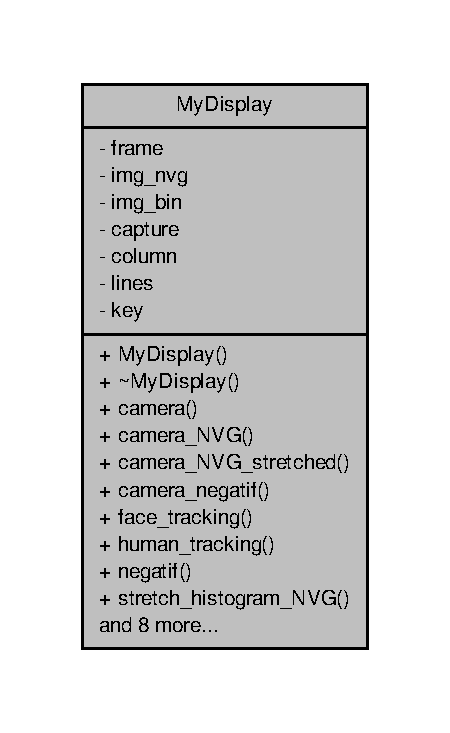
\includegraphics[width=216pt]{classMyDisplay__coll__graph}
\end{center}
\end{figure}
\subsection*{Public Member Functions}
\begin{DoxyCompactItemize}
\item 
\hyperlink{classMyDisplay_aaf21029e4055eaadf1d750514b3b800a}{My\-Display} ()
\item 
\hyperlink{classMyDisplay_ac60f1fded498f57332783a5b66264c8c}{$\sim$\-My\-Display} ()
\item 
void \hyperlink{classMyDisplay_a00b712ee117708d620dc80d84d3e7281}{camera} ()
\item 
void \hyperlink{classMyDisplay_abfe046ec64aef3f9487e76c5a523bb48}{camera\-\_\-\-N\-V\-G} ()
\item 
void \hyperlink{classMyDisplay_a15661db4339f486356e93716c65a3a7a}{camera\-\_\-\-N\-V\-G\-\_\-stretched} ()
\item 
void \hyperlink{classMyDisplay_ac2ce70a95b5dd437951d3ebc7f3756d3}{camera\-\_\-negatif} ()
\item 
void \hyperlink{classMyDisplay_a8033377d23dca5526634eded73efb902}{face\-\_\-tracking} ()
\item 
void \hyperlink{classMyDisplay_a23cd838f0f2300db6370334ab60b99e6}{human\-\_\-tracking} ()
\item 
void \hyperlink{classMyDisplay_aed313dcbb8592f0786479321ebcadb54}{negatif} (Ipl\-Image $\ast$image)
\item 
void \hyperlink{classMyDisplay_a62ac61c3751293a48dad6a7254d039c0}{stretch\-\_\-histogram\-\_\-\-N\-V\-G} (Ipl\-Image $\ast$image)
\item 
void \hyperlink{classMyDisplay_a85d57087410b57368b92661fc63a6488}{detect\-\_\-faces} (Cv\-Haar\-Classifier\-Cascade $\ast$cascade, Cv\-Mem\-Storage $\ast$storage)
\item 
void \hyperlink{classMyDisplay_acbd50379c2ac9d3a275699550ba8530d}{detect\-\_\-human} (Cv\-Haar\-Classifier\-Cascade $\ast$cascade, Cv\-Mem\-Storage $\ast$storage)
\item 
Ipl\-Image $\ast$ \hyperlink{classMyDisplay_abc01f4d82f8eb6fffbc479fd56b7630e}{image\-\_\-camera} (Cv\-Capture $\ast$\hyperlink{classMyDisplay_aa2d469497bae80c2dc6596542a6af041}{capture})
\item 
Ipl\-Image $\ast$ \hyperlink{classMyDisplay_a745b42e0c45958feb46783864c53ecd2}{image\-\_\-camera\-\_\-\-N\-V\-G} (Cv\-Capture $\ast$\hyperlink{classMyDisplay_aa2d469497bae80c2dc6596542a6af041}{capture})
\item 
Ipl\-Image $\ast$ \hyperlink{classMyDisplay_a661a4a4884d246002faf8044e0975312}{image\-\_\-camera\-\_\-\-N\-V\-G\-\_\-stretched} (Cv\-Capture $\ast$\hyperlink{classMyDisplay_aa2d469497bae80c2dc6596542a6af041}{capture})
\item 
Ipl\-Image $\ast$ \hyperlink{classMyDisplay_a19fca82a8e9441c154a3d1ed4fbc261a}{image\-\_\-camera\-\_\-negatif} (Cv\-Capture $\ast$\hyperlink{classMyDisplay_aa2d469497bae80c2dc6596542a6af041}{capture})
\item 
Ipl\-Image $\ast$ \hyperlink{classMyDisplay_ad1c456244088d6282726143224c112e0}{image\-\_\-face\-\_\-tracking} (Cv\-Capture $\ast$\hyperlink{classMyDisplay_aa2d469497bae80c2dc6596542a6af041}{capture})
\item 
Ipl\-Image $\ast$ \hyperlink{classMyDisplay_ae08642f4d5698ff0d25b9e03765db55b}{image\-\_\-human\-\_\-tracking} (Cv\-Capture $\ast$\hyperlink{classMyDisplay_aa2d469497bae80c2dc6596542a6af041}{capture})
\end{DoxyCompactItemize}
\subsection*{Private Attributes}
\begin{DoxyCompactItemize}
\item 
Ipl\-Image $\ast$ \hyperlink{classMyDisplay_aee26cb4ae47e963a1491466d08a27d0c}{frame} = N\-U\-L\-L
\item 
Ipl\-Image $\ast$ \hyperlink{classMyDisplay_a66ed19ac74896c2fef063f853a80416f}{img\-\_\-nvg} = N\-U\-L\-L
\item 
Ipl\-Image $\ast$ \hyperlink{classMyDisplay_aaa25208b5bfada51a5ac878f76453f44}{img\-\_\-bin} = N\-U\-L\-L
\item 
Cv\-Capture $\ast$ \hyperlink{classMyDisplay_aa2d469497bae80c2dc6596542a6af041}{capture} = N\-U\-L\-L
\item 
int \hyperlink{classMyDisplay_a94a51f56cd8e8c5b6e22f5634b5d5f12}{column} = 0
\item 
int \hyperlink{classMyDisplay_a2cb48c4b915895b0bc7e7cd0f524a3be}{lines} = 0
\item 
int \hyperlink{classMyDisplay_af7602dfb0020925158d89532de80135e}{key} = 0
\end{DoxyCompactItemize}


\subsection{Detailed Description}


Definition at line 8 of file mydisplay.\-h.



\subsection{Constructor \& Destructor Documentation}
\hypertarget{classMyDisplay_aaf21029e4055eaadf1d750514b3b800a}{\index{My\-Display@{My\-Display}!My\-Display@{My\-Display}}
\index{My\-Display@{My\-Display}!MyDisplay@{My\-Display}}
\subsubsection[{My\-Display}]{\setlength{\rightskip}{0pt plus 5cm}My\-Display\-::\-My\-Display (
\begin{DoxyParamCaption}
{}
\end{DoxyParamCaption}
)}}\label{classMyDisplay_aaf21029e4055eaadf1d750514b3b800a}


Definition at line 12 of file mydisplay.\-cpp.


\begin{DoxyCode}
\{
\}
\end{DoxyCode}
\hypertarget{classMyDisplay_ac60f1fded498f57332783a5b66264c8c}{\index{My\-Display@{My\-Display}!$\sim$\-My\-Display@{$\sim$\-My\-Display}}
\index{$\sim$\-My\-Display@{$\sim$\-My\-Display}!MyDisplay@{My\-Display}}
\subsubsection[{$\sim$\-My\-Display}]{\setlength{\rightskip}{0pt plus 5cm}My\-Display\-::$\sim$\-My\-Display (
\begin{DoxyParamCaption}
{}
\end{DoxyParamCaption}
)}}\label{classMyDisplay_ac60f1fded498f57332783a5b66264c8c}


Definition at line 17 of file mydisplay.\-cpp.


\begin{DoxyCode}
\{
\}
\end{DoxyCode}


\subsection{Member Function Documentation}
\hypertarget{classMyDisplay_a00b712ee117708d620dc80d84d3e7281}{\index{My\-Display@{My\-Display}!camera@{camera}}
\index{camera@{camera}!MyDisplay@{My\-Display}}
\subsubsection[{camera}]{\setlength{\rightskip}{0pt plus 5cm}void My\-Display\-::camera (
\begin{DoxyParamCaption}
{}
\end{DoxyParamCaption}
)}}\label{classMyDisplay_a00b712ee117708d620dc80d84d3e7281}


Definition at line 21 of file mydisplay.\-cpp.



References capture, frame, and key.


\begin{DoxyCode}
\{
    IplImage* \hyperlink{classMyDisplay_aee26cb4ae47e963a1491466d08a27d0c}{frame} = NULL;
    CvCapture *\hyperlink{classMyDisplay_aa2d469497bae80c2dc6596542a6af041}{capture} = cvCreateCameraCapture(CV\_CAP\_ANY);
    \textcolor{keywordflow}{while} (1)\{
        frame = cvQueryFrame(capture);
        cvShowImage(\textcolor{stringliteral}{"test"}, frame);
        \textcolor{keywordtype}{int} \hyperlink{classMyDisplay_af7602dfb0020925158d89532de80135e}{key} = cvWaitKey(1);
        \textcolor{keywordflow}{if} (key == \textcolor{charliteral}{'q'})
        \{
            \textcolor{keywordflow}{break};
        \}
        \textcolor{keywordflow}{else} \{
            \textcolor{comment}{//nothing to do}
        \}
    \}
    cvReleaseCapture(&capture);
\}
\end{DoxyCode}
\hypertarget{classMyDisplay_ac2ce70a95b5dd437951d3ebc7f3756d3}{\index{My\-Display@{My\-Display}!camera\-\_\-negatif@{camera\-\_\-negatif}}
\index{camera\-\_\-negatif@{camera\-\_\-negatif}!MyDisplay@{My\-Display}}
\subsubsection[{camera\-\_\-negatif}]{\setlength{\rightskip}{0pt plus 5cm}void My\-Display\-::camera\-\_\-negatif (
\begin{DoxyParamCaption}
{}
\end{DoxyParamCaption}
)}}\label{classMyDisplay_ac2ce70a95b5dd437951d3ebc7f3756d3}


Definition at line 161 of file mydisplay.\-cpp.



References capture, frame, img\-\_\-nvg, key, negatif(), and stretch\-\_\-histogram\-\_\-\-N\-V\-G().


\begin{DoxyCode}
\{
    \hyperlink{classMyDisplay_aa2d469497bae80c2dc6596542a6af041}{capture} = cvCreateCameraCapture(CV\_CAP\_ANY);
    \textcolor{keywordflow}{while} (1)\{
        \hyperlink{classMyDisplay_aee26cb4ae47e963a1491466d08a27d0c}{frame} = cvQueryFrame(\hyperlink{classMyDisplay_aa2d469497bae80c2dc6596542a6af041}{capture});
        \hyperlink{classMyDisplay_a66ed19ac74896c2fef063f853a80416f}{img\_nvg} = cvCreateImage(cvGetSize(\hyperlink{classMyDisplay_aee26cb4ae47e963a1491466d08a27d0c}{frame}), \hyperlink{classMyDisplay_aee26cb4ae47e963a1491466d08a27d0c}{frame}->depth
      , 1);

        \textcolor{comment}{//conversion en niveau de gris}
        cvConvertImage(\hyperlink{classMyDisplay_aee26cb4ae47e963a1491466d08a27d0c}{frame}, \hyperlink{classMyDisplay_a66ed19ac74896c2fef063f853a80416f}{img\_nvg}, 0);

        \hyperlink{classMyDisplay_a62ac61c3751293a48dad6a7254d039c0}{stretch\_histogram\_NVG}(\hyperlink{classMyDisplay_a66ed19ac74896c2fef063f853a80416f}{img\_nvg});
        \hyperlink{classMyDisplay_aed313dcbb8592f0786479321ebcadb54}{negatif}(\hyperlink{classMyDisplay_a66ed19ac74896c2fef063f853a80416f}{img\_nvg});

        \textcolor{comment}{//frame = negatif(frame);}
        cvShowImage(\textcolor{stringliteral}{"test"}, \hyperlink{classMyDisplay_a66ed19ac74896c2fef063f853a80416f}{img\_nvg});
        \textcolor{keywordtype}{int} \hyperlink{classMyDisplay_af7602dfb0020925158d89532de80135e}{key} = cvWaitKey(1);
        \textcolor{keywordflow}{if} (key == \textcolor{charliteral}{'q'})
        \{
            \textcolor{keywordflow}{break};
        \}
        \textcolor{keywordflow}{else} \{
            \textcolor{comment}{//nothing to do}
        \}
    \}
    cvReleaseCapture(&\hyperlink{classMyDisplay_aa2d469497bae80c2dc6596542a6af041}{capture});

\}
\end{DoxyCode}
\hypertarget{classMyDisplay_abfe046ec64aef3f9487e76c5a523bb48}{\index{My\-Display@{My\-Display}!camera\-\_\-\-N\-V\-G@{camera\-\_\-\-N\-V\-G}}
\index{camera\-\_\-\-N\-V\-G@{camera\-\_\-\-N\-V\-G}!MyDisplay@{My\-Display}}
\subsubsection[{camera\-\_\-\-N\-V\-G}]{\setlength{\rightskip}{0pt plus 5cm}void My\-Display\-::camera\-\_\-\-N\-V\-G (
\begin{DoxyParamCaption}
{}
\end{DoxyParamCaption}
)}}\label{classMyDisplay_abfe046ec64aef3f9487e76c5a523bb48}


Definition at line 40 of file mydisplay.\-cpp.



References capture, frame, img\-\_\-nvg, and key.


\begin{DoxyCode}
\{
    \hyperlink{classMyDisplay_aa2d469497bae80c2dc6596542a6af041}{capture} = cvCreateCameraCapture(CV\_CAP\_ANY);
    \textcolor{keywordflow}{while} (1)\{
        \hyperlink{classMyDisplay_aee26cb4ae47e963a1491466d08a27d0c}{frame} = cvQueryFrame(\hyperlink{classMyDisplay_aa2d469497bae80c2dc6596542a6af041}{capture});
        \hyperlink{classMyDisplay_a66ed19ac74896c2fef063f853a80416f}{img\_nvg} = cvCreateImage(cvGetSize(\hyperlink{classMyDisplay_aee26cb4ae47e963a1491466d08a27d0c}{frame}), \hyperlink{classMyDisplay_aee26cb4ae47e963a1491466d08a27d0c}{frame}->depth
      , 1);

        \textcolor{comment}{//conversion en niveau de gris}
        cvConvertImage(\hyperlink{classMyDisplay_aee26cb4ae47e963a1491466d08a27d0c}{frame}, \hyperlink{classMyDisplay_a66ed19ac74896c2fef063f853a80416f}{img\_nvg}, 0);

        cvShowImage(\textcolor{stringliteral}{"test"}, \hyperlink{classMyDisplay_a66ed19ac74896c2fef063f853a80416f}{img\_nvg});
        \textcolor{keywordtype}{int} \hyperlink{classMyDisplay_af7602dfb0020925158d89532de80135e}{key} = cvWaitKey(1);
        \textcolor{keywordflow}{if} (key == \textcolor{charliteral}{'q'})
        \{
            \textcolor{keywordflow}{break};
        \}
        \textcolor{keywordflow}{else} \{
            \textcolor{comment}{//nothing to do}
        \}
    \}
    cvReleaseCapture(&\hyperlink{classMyDisplay_aa2d469497bae80c2dc6596542a6af041}{capture});
\}
\end{DoxyCode}
\hypertarget{classMyDisplay_a15661db4339f486356e93716c65a3a7a}{\index{My\-Display@{My\-Display}!camera\-\_\-\-N\-V\-G\-\_\-stretched@{camera\-\_\-\-N\-V\-G\-\_\-stretched}}
\index{camera\-\_\-\-N\-V\-G\-\_\-stretched@{camera\-\_\-\-N\-V\-G\-\_\-stretched}!MyDisplay@{My\-Display}}
\subsubsection[{camera\-\_\-\-N\-V\-G\-\_\-stretched}]{\setlength{\rightskip}{0pt plus 5cm}void My\-Display\-::camera\-\_\-\-N\-V\-G\-\_\-stretched (
\begin{DoxyParamCaption}
{}
\end{DoxyParamCaption}
)}}\label{classMyDisplay_a15661db4339f486356e93716c65a3a7a}


Definition at line 121 of file mydisplay.\-cpp.



References capture, frame, img\-\_\-nvg, key, and stretch\-\_\-histogram\-\_\-\-N\-V\-G().


\begin{DoxyCode}
\{
    \hyperlink{classMyDisplay_aa2d469497bae80c2dc6596542a6af041}{capture} = cvCreateCameraCapture(CV\_CAP\_ANY);
    \textcolor{keywordflow}{while} (1)\{
        \hyperlink{classMyDisplay_aee26cb4ae47e963a1491466d08a27d0c}{frame} = cvQueryFrame(\hyperlink{classMyDisplay_aa2d469497bae80c2dc6596542a6af041}{capture});
        \hyperlink{classMyDisplay_a66ed19ac74896c2fef063f853a80416f}{img\_nvg} = cvCreateImage(cvGetSize(\hyperlink{classMyDisplay_aee26cb4ae47e963a1491466d08a27d0c}{frame}), \hyperlink{classMyDisplay_aee26cb4ae47e963a1491466d08a27d0c}{frame}->depth
      , 1);

        \textcolor{comment}{//conversion en niveau de gris}
        cvConvertImage(\hyperlink{classMyDisplay_aee26cb4ae47e963a1491466d08a27d0c}{frame}, \hyperlink{classMyDisplay_a66ed19ac74896c2fef063f853a80416f}{img\_nvg}, 0);

        \hyperlink{classMyDisplay_a62ac61c3751293a48dad6a7254d039c0}{stretch\_histogram\_NVG}(\hyperlink{classMyDisplay_a66ed19ac74896c2fef063f853a80416f}{img\_nvg});

        cvShowImage(\textcolor{stringliteral}{"test"}, \hyperlink{classMyDisplay_a66ed19ac74896c2fef063f853a80416f}{img\_nvg});
        \textcolor{keywordtype}{int} \hyperlink{classMyDisplay_af7602dfb0020925158d89532de80135e}{key} = cvWaitKey(1);
        \textcolor{keywordflow}{if} (key == \textcolor{charliteral}{'q'})
        \{
            \textcolor{keywordflow}{break};
        \}
        \textcolor{keywordflow}{else} \{
            \textcolor{comment}{//nothing to do}
        \}
    \}
    cvReleaseCapture(&\hyperlink{classMyDisplay_aa2d469497bae80c2dc6596542a6af041}{capture});
\}
\end{DoxyCode}
\hypertarget{classMyDisplay_a85d57087410b57368b92661fc63a6488}{\index{My\-Display@{My\-Display}!detect\-\_\-faces@{detect\-\_\-faces}}
\index{detect\-\_\-faces@{detect\-\_\-faces}!MyDisplay@{My\-Display}}
\subsubsection[{detect\-\_\-faces}]{\setlength{\rightskip}{0pt plus 5cm}void My\-Display\-::detect\-\_\-faces (
\begin{DoxyParamCaption}
\item[{Cv\-Haar\-Classifier\-Cascade $\ast$}]{cascade, }
\item[{Cv\-Mem\-Storage $\ast$}]{storage}
\end{DoxyParamCaption}
)}}\label{classMyDisplay_a85d57087410b57368b92661fc63a6488}
\hypertarget{classMyDisplay_acbd50379c2ac9d3a275699550ba8530d}{\index{My\-Display@{My\-Display}!detect\-\_\-human@{detect\-\_\-human}}
\index{detect\-\_\-human@{detect\-\_\-human}!MyDisplay@{My\-Display}}
\subsubsection[{detect\-\_\-human}]{\setlength{\rightskip}{0pt plus 5cm}void My\-Display\-::detect\-\_\-human (
\begin{DoxyParamCaption}
\item[{Cv\-Haar\-Classifier\-Cascade $\ast$}]{cascade, }
\item[{Cv\-Mem\-Storage $\ast$}]{storage}
\end{DoxyParamCaption}
)}}\label{classMyDisplay_acbd50379c2ac9d3a275699550ba8530d}
\hypertarget{classMyDisplay_a8033377d23dca5526634eded73efb902}{\index{My\-Display@{My\-Display}!face\-\_\-tracking@{face\-\_\-tracking}}
\index{face\-\_\-tracking@{face\-\_\-tracking}!MyDisplay@{My\-Display}}
\subsubsection[{face\-\_\-tracking}]{\setlength{\rightskip}{0pt plus 5cm}void My\-Display\-::face\-\_\-tracking (
\begin{DoxyParamCaption}
{}
\end{DoxyParamCaption}
)}}\label{classMyDisplay_a8033377d23dca5526634eded73efb902}
\hypertarget{classMyDisplay_a23cd838f0f2300db6370334ab60b99e6}{\index{My\-Display@{My\-Display}!human\-\_\-tracking@{human\-\_\-tracking}}
\index{human\-\_\-tracking@{human\-\_\-tracking}!MyDisplay@{My\-Display}}
\subsubsection[{human\-\_\-tracking}]{\setlength{\rightskip}{0pt plus 5cm}void My\-Display\-::human\-\_\-tracking (
\begin{DoxyParamCaption}
{}
\end{DoxyParamCaption}
)}}\label{classMyDisplay_a23cd838f0f2300db6370334ab60b99e6}
\hypertarget{classMyDisplay_abc01f4d82f8eb6fffbc479fd56b7630e}{\index{My\-Display@{My\-Display}!image\-\_\-camera@{image\-\_\-camera}}
\index{image\-\_\-camera@{image\-\_\-camera}!MyDisplay@{My\-Display}}
\subsubsection[{image\-\_\-camera}]{\setlength{\rightskip}{0pt plus 5cm}Ipl\-Image $\ast$ My\-Display\-::image\-\_\-camera (
\begin{DoxyParamCaption}
\item[{Cv\-Capture $\ast$}]{capture}
\end{DoxyParamCaption}
)}}\label{classMyDisplay_abc01f4d82f8eb6fffbc479fd56b7630e}


Definition at line 331 of file mydisplay.\-cpp.



References frame.


\begin{DoxyCode}
\{
    IplImage* \hyperlink{classMyDisplay_aee26cb4ae47e963a1491466d08a27d0c}{frame} = NULL;
    frame = cvQueryFrame(\hyperlink{classMyDisplay_aa2d469497bae80c2dc6596542a6af041}{capture});
    \textcolor{keywordflow}{return} \hyperlink{classMyDisplay_aee26cb4ae47e963a1491466d08a27d0c}{frame};
\}
\end{DoxyCode}
\hypertarget{classMyDisplay_a19fca82a8e9441c154a3d1ed4fbc261a}{\index{My\-Display@{My\-Display}!image\-\_\-camera\-\_\-negatif@{image\-\_\-camera\-\_\-negatif}}
\index{image\-\_\-camera\-\_\-negatif@{image\-\_\-camera\-\_\-negatif}!MyDisplay@{My\-Display}}
\subsubsection[{image\-\_\-camera\-\_\-negatif}]{\setlength{\rightskip}{0pt plus 5cm}Ipl\-Image $\ast$ My\-Display\-::image\-\_\-camera\-\_\-negatif (
\begin{DoxyParamCaption}
\item[{Cv\-Capture $\ast$}]{capture}
\end{DoxyParamCaption}
)}}\label{classMyDisplay_a19fca82a8e9441c154a3d1ed4fbc261a}


Definition at line 362 of file mydisplay.\-cpp.



References frame, img\-\_\-nvg, negatif(), and stretch\-\_\-histogram\-\_\-\-N\-V\-G().


\begin{DoxyCode}
\{

    \hyperlink{classMyDisplay_aee26cb4ae47e963a1491466d08a27d0c}{frame} = cvQueryFrame(\hyperlink{classMyDisplay_aa2d469497bae80c2dc6596542a6af041}{capture});
    \hyperlink{classMyDisplay_a66ed19ac74896c2fef063f853a80416f}{img\_nvg} = cvCreateImage(cvGetSize(\hyperlink{classMyDisplay_aee26cb4ae47e963a1491466d08a27d0c}{frame}), \hyperlink{classMyDisplay_aee26cb4ae47e963a1491466d08a27d0c}{frame}->depth, 1)
      ;

    \textcolor{comment}{//conversion en niveau de gris}
    cvConvertImage(\hyperlink{classMyDisplay_aee26cb4ae47e963a1491466d08a27d0c}{frame}, \hyperlink{classMyDisplay_a66ed19ac74896c2fef063f853a80416f}{img\_nvg}, 0);

    \hyperlink{classMyDisplay_a62ac61c3751293a48dad6a7254d039c0}{stretch\_histogram\_NVG}(\hyperlink{classMyDisplay_a66ed19ac74896c2fef063f853a80416f}{img\_nvg});
    \hyperlink{classMyDisplay_aed313dcbb8592f0786479321ebcadb54}{negatif}(\hyperlink{classMyDisplay_a66ed19ac74896c2fef063f853a80416f}{img\_nvg});
    \textcolor{keywordflow}{return} \hyperlink{classMyDisplay_a66ed19ac74896c2fef063f853a80416f}{img\_nvg};
\}
\end{DoxyCode}
\hypertarget{classMyDisplay_a745b42e0c45958feb46783864c53ecd2}{\index{My\-Display@{My\-Display}!image\-\_\-camera\-\_\-\-N\-V\-G@{image\-\_\-camera\-\_\-\-N\-V\-G}}
\index{image\-\_\-camera\-\_\-\-N\-V\-G@{image\-\_\-camera\-\_\-\-N\-V\-G}!MyDisplay@{My\-Display}}
\subsubsection[{image\-\_\-camera\-\_\-\-N\-V\-G}]{\setlength{\rightskip}{0pt plus 5cm}Ipl\-Image $\ast$ My\-Display\-::image\-\_\-camera\-\_\-\-N\-V\-G (
\begin{DoxyParamCaption}
\item[{Cv\-Capture $\ast$}]{capture}
\end{DoxyParamCaption}
)}}\label{classMyDisplay_a745b42e0c45958feb46783864c53ecd2}


Definition at line 338 of file mydisplay.\-cpp.



References frame, and img\-\_\-nvg.


\begin{DoxyCode}
\{
    \hyperlink{classMyDisplay_aee26cb4ae47e963a1491466d08a27d0c}{frame} = cvQueryFrame(\hyperlink{classMyDisplay_aa2d469497bae80c2dc6596542a6af041}{capture});
    \hyperlink{classMyDisplay_a66ed19ac74896c2fef063f853a80416f}{img\_nvg} = cvCreateImage(cvGetSize(\hyperlink{classMyDisplay_aee26cb4ae47e963a1491466d08a27d0c}{frame}), \hyperlink{classMyDisplay_aee26cb4ae47e963a1491466d08a27d0c}{frame}->depth, 1)
      ;

    \textcolor{comment}{//conversion en niveau de gris}
    cvConvertImage(\hyperlink{classMyDisplay_aee26cb4ae47e963a1491466d08a27d0c}{frame}, \hyperlink{classMyDisplay_a66ed19ac74896c2fef063f853a80416f}{img\_nvg}, 0);
    \textcolor{keywordflow}{return} \hyperlink{classMyDisplay_aee26cb4ae47e963a1491466d08a27d0c}{frame};
\}
\end{DoxyCode}
\hypertarget{classMyDisplay_a661a4a4884d246002faf8044e0975312}{\index{My\-Display@{My\-Display}!image\-\_\-camera\-\_\-\-N\-V\-G\-\_\-stretched@{image\-\_\-camera\-\_\-\-N\-V\-G\-\_\-stretched}}
\index{image\-\_\-camera\-\_\-\-N\-V\-G\-\_\-stretched@{image\-\_\-camera\-\_\-\-N\-V\-G\-\_\-stretched}!MyDisplay@{My\-Display}}
\subsubsection[{image\-\_\-camera\-\_\-\-N\-V\-G\-\_\-stretched}]{\setlength{\rightskip}{0pt plus 5cm}Ipl\-Image $\ast$ My\-Display\-::image\-\_\-camera\-\_\-\-N\-V\-G\-\_\-stretched (
\begin{DoxyParamCaption}
\item[{Cv\-Capture $\ast$}]{capture}
\end{DoxyParamCaption}
)}}\label{classMyDisplay_a661a4a4884d246002faf8044e0975312}


Definition at line 348 of file mydisplay.\-cpp.



References frame, img\-\_\-nvg, and stretch\-\_\-histogram\-\_\-\-N\-V\-G().


\begin{DoxyCode}
\{

    \hyperlink{classMyDisplay_aee26cb4ae47e963a1491466d08a27d0c}{frame} = cvQueryFrame(\hyperlink{classMyDisplay_aa2d469497bae80c2dc6596542a6af041}{capture});
    \hyperlink{classMyDisplay_a66ed19ac74896c2fef063f853a80416f}{img\_nvg} = cvCreateImage(cvGetSize(\hyperlink{classMyDisplay_aee26cb4ae47e963a1491466d08a27d0c}{frame}), \hyperlink{classMyDisplay_aee26cb4ae47e963a1491466d08a27d0c}{frame}->depth, 1)
      ;

    \textcolor{comment}{//conversion en niveau de gris}
    cvConvertImage(\hyperlink{classMyDisplay_aee26cb4ae47e963a1491466d08a27d0c}{frame}, \hyperlink{classMyDisplay_a66ed19ac74896c2fef063f853a80416f}{img\_nvg}, 0);

    \hyperlink{classMyDisplay_a62ac61c3751293a48dad6a7254d039c0}{stretch\_histogram\_NVG}(\hyperlink{classMyDisplay_a66ed19ac74896c2fef063f853a80416f}{img\_nvg});

    \textcolor{keywordflow}{return} \hyperlink{classMyDisplay_a66ed19ac74896c2fef063f853a80416f}{img\_nvg};
\}
\end{DoxyCode}
\hypertarget{classMyDisplay_ad1c456244088d6282726143224c112e0}{\index{My\-Display@{My\-Display}!image\-\_\-face\-\_\-tracking@{image\-\_\-face\-\_\-tracking}}
\index{image\-\_\-face\-\_\-tracking@{image\-\_\-face\-\_\-tracking}!MyDisplay@{My\-Display}}
\subsubsection[{image\-\_\-face\-\_\-tracking}]{\setlength{\rightskip}{0pt plus 5cm}Ipl\-Image$\ast$ My\-Display\-::image\-\_\-face\-\_\-tracking (
\begin{DoxyParamCaption}
\item[{Cv\-Capture $\ast$}]{capture}
\end{DoxyParamCaption}
)}}\label{classMyDisplay_ad1c456244088d6282726143224c112e0}
\hypertarget{classMyDisplay_ae08642f4d5698ff0d25b9e03765db55b}{\index{My\-Display@{My\-Display}!image\-\_\-human\-\_\-tracking@{image\-\_\-human\-\_\-tracking}}
\index{image\-\_\-human\-\_\-tracking@{image\-\_\-human\-\_\-tracking}!MyDisplay@{My\-Display}}
\subsubsection[{image\-\_\-human\-\_\-tracking}]{\setlength{\rightskip}{0pt plus 5cm}Ipl\-Image$\ast$ My\-Display\-::image\-\_\-human\-\_\-tracking (
\begin{DoxyParamCaption}
\item[{Cv\-Capture $\ast$}]{capture}
\end{DoxyParamCaption}
)}}\label{classMyDisplay_ae08642f4d5698ff0d25b9e03765db55b}
\hypertarget{classMyDisplay_aed313dcbb8592f0786479321ebcadb54}{\index{My\-Display@{My\-Display}!negatif@{negatif}}
\index{negatif@{negatif}!MyDisplay@{My\-Display}}
\subsubsection[{negatif}]{\setlength{\rightskip}{0pt plus 5cm}void My\-Display\-::negatif (
\begin{DoxyParamCaption}
\item[{Ipl\-Image $\ast$}]{image}
\end{DoxyParamCaption}
)}}\label{classMyDisplay_aed313dcbb8592f0786479321ebcadb54}


Definition at line 146 of file mydisplay.\-cpp.



References column, and lines.



Referenced by camera\-\_\-negatif(), and image\-\_\-camera\-\_\-negatif().


\begin{DoxyCode}
\{
    CvScalar scalar\_return;

    \textcolor{keywordflow}{for} (\hyperlink{classMyDisplay_a94a51f56cd8e8c5b6e22f5634b5d5f12}{column} = 0; \hyperlink{classMyDisplay_a94a51f56cd8e8c5b6e22f5634b5d5f12}{column} < image->width; \hyperlink{classMyDisplay_a94a51f56cd8e8c5b6e22f5634b5d5f12}{column}++)
    \{
        \textcolor{keywordflow}{for} (\hyperlink{classMyDisplay_a2cb48c4b915895b0bc7e7cd0f524a3be}{lines} = 0; \hyperlink{classMyDisplay_a2cb48c4b915895b0bc7e7cd0f524a3be}{lines} < image->height; \hyperlink{classMyDisplay_a2cb48c4b915895b0bc7e7cd0f524a3be}{lines}++)
        \{
            scalar\_return = cvGet2D(image, \hyperlink{classMyDisplay_a2cb48c4b915895b0bc7e7cd0f524a3be}{lines}, \hyperlink{classMyDisplay_a94a51f56cd8e8c5b6e22f5634b5d5f12}{column});
            scalar\_return.val[0] = 255 - scalar\_return.val[0];
            cvSet2D(image, \hyperlink{classMyDisplay_a2cb48c4b915895b0bc7e7cd0f524a3be}{lines}, \hyperlink{classMyDisplay_a94a51f56cd8e8c5b6e22f5634b5d5f12}{column}, scalar\_return);
        \}
    \}
\}
\end{DoxyCode}
\hypertarget{classMyDisplay_a62ac61c3751293a48dad6a7254d039c0}{\index{My\-Display@{My\-Display}!stretch\-\_\-histogram\-\_\-\-N\-V\-G@{stretch\-\_\-histogram\-\_\-\-N\-V\-G}}
\index{stretch\-\_\-histogram\-\_\-\-N\-V\-G@{stretch\-\_\-histogram\-\_\-\-N\-V\-G}!MyDisplay@{My\-Display}}
\subsubsection[{stretch\-\_\-histogram\-\_\-\-N\-V\-G}]{\setlength{\rightskip}{0pt plus 5cm}void My\-Display\-::stretch\-\_\-histogram\-\_\-\-N\-V\-G (
\begin{DoxyParamCaption}
\item[{Ipl\-Image $\ast$}]{image}
\end{DoxyParamCaption}
)}}\label{classMyDisplay_a62ac61c3751293a48dad6a7254d039c0}


Definition at line 63 of file mydisplay.\-cpp.



References column, and lines.



Referenced by camera\-\_\-negatif(), camera\-\_\-\-N\-V\-G\-\_\-stretched(), image\-\_\-camera\-\_\-negatif(), and image\-\_\-camera\-\_\-\-N\-V\-G\-\_\-stretched().


\begin{DoxyCode}
\{
    \textcolor{comment}{//if the picture is in NVG}
    \textcolor{keywordflow}{if} (image->nChannels != 1)
    \{
        \textcolor{keywordflow}{return};
    \}
    \textcolor{keywordflow}{else} \{
        \textcolor{comment}{//nothing to do}
    \}

    \textcolor{comment}{// fix the max and min for the mathematic function}
    \textcolor{keywordtype}{int} pix\_min = 255;
    \textcolor{keywordtype}{int} pix\_max = 0;

    CvScalar scalaire;

    \textcolor{comment}{//we search pix\_min and pix\_max}
    \textcolor{keywordflow}{for} (\hyperlink{classMyDisplay_a94a51f56cd8e8c5b6e22f5634b5d5f12}{column} = 0; \hyperlink{classMyDisplay_a94a51f56cd8e8c5b6e22f5634b5d5f12}{column} < image->width; \hyperlink{classMyDisplay_a94a51f56cd8e8c5b6e22f5634b5d5f12}{column}++)
    \{
        \textcolor{keywordflow}{for} (\hyperlink{classMyDisplay_a2cb48c4b915895b0bc7e7cd0f524a3be}{lines} = 0; \hyperlink{classMyDisplay_a2cb48c4b915895b0bc7e7cd0f524a3be}{lines} < image->height; \hyperlink{classMyDisplay_a2cb48c4b915895b0bc7e7cd0f524a3be}{lines}++)
        \{
            \textcolor{comment}{//we take the pixel or scalaire}
            scalaire = cvGet2D(image, \hyperlink{classMyDisplay_a2cb48c4b915895b0bc7e7cd0f524a3be}{lines}, \hyperlink{classMyDisplay_a94a51f56cd8e8c5b6e22f5634b5d5f12}{column});

            \textcolor{comment}{//we search extremums}
            \textcolor{keywordflow}{if} (scalaire.val[0] < pix\_min)
            \{
                pix\_min = (int)scalaire.val[0];
            \}
            \textcolor{keywordflow}{else} \textcolor{keywordflow}{if} (scalaire.val[0] > pix\_max)
            \{
                pix\_max = (int)scalaire.val[0];
            \}
            \textcolor{keywordflow}{else} \{
                \textcolor{comment}{//nothing to do}
            \}
        \}
    \}

    \textcolor{comment}{//we have max and min, we normalize}
    \textcolor{keywordflow}{for} (\hyperlink{classMyDisplay_a94a51f56cd8e8c5b6e22f5634b5d5f12}{column} = 0; \hyperlink{classMyDisplay_a94a51f56cd8e8c5b6e22f5634b5d5f12}{column} < image->width; \hyperlink{classMyDisplay_a94a51f56cd8e8c5b6e22f5634b5d5f12}{column}++)
    \{
        \textcolor{keywordflow}{for} (\hyperlink{classMyDisplay_a2cb48c4b915895b0bc7e7cd0f524a3be}{lines} = 0; \hyperlink{classMyDisplay_a2cb48c4b915895b0bc7e7cd0f524a3be}{lines} < image->height; \hyperlink{classMyDisplay_a2cb48c4b915895b0bc7e7cd0f524a3be}{lines}++)
        \{
            \textcolor{comment}{//we take the pixel or scalaire}
            scalaire = cvGet2D(image, \hyperlink{classMyDisplay_a2cb48c4b915895b0bc7e7cd0f524a3be}{lines}, \hyperlink{classMyDisplay_a94a51f56cd8e8c5b6e22f5634b5d5f12}{column});

            \textcolor{comment}{//Normalize with mathematic equation}
            scalaire.val[0] = 255 * (scalaire.val[0] - pix\_min);
            scalaire.val[0] = scalaire.val[0] / (pix\_max - pix\_min);

            \textcolor{comment}{//we replace the pixel in the picture}
            cvSet2D(image, \hyperlink{classMyDisplay_a2cb48c4b915895b0bc7e7cd0f524a3be}{lines}, \hyperlink{classMyDisplay_a94a51f56cd8e8c5b6e22f5634b5d5f12}{column}, scalaire);
        \}
    \}
\}
\end{DoxyCode}


\subsection{Member Data Documentation}
\hypertarget{classMyDisplay_aa2d469497bae80c2dc6596542a6af041}{\index{My\-Display@{My\-Display}!capture@{capture}}
\index{capture@{capture}!MyDisplay@{My\-Display}}
\subsubsection[{capture}]{\setlength{\rightskip}{0pt plus 5cm}Cv\-Capture$\ast$ My\-Display\-::capture = N\-U\-L\-L\hspace{0.3cm}{\ttfamily [private]}}}\label{classMyDisplay_aa2d469497bae80c2dc6596542a6af041}


Definition at line 48 of file mydisplay.\-h.



Referenced by camera(), camera\-\_\-negatif(), camera\-\_\-\-N\-V\-G(), and camera\-\_\-\-N\-V\-G\-\_\-stretched().

\hypertarget{classMyDisplay_a94a51f56cd8e8c5b6e22f5634b5d5f12}{\index{My\-Display@{My\-Display}!column@{column}}
\index{column@{column}!MyDisplay@{My\-Display}}
\subsubsection[{column}]{\setlength{\rightskip}{0pt plus 5cm}int My\-Display\-::column = 0\hspace{0.3cm}{\ttfamily [private]}}}\label{classMyDisplay_a94a51f56cd8e8c5b6e22f5634b5d5f12}


Definition at line 49 of file mydisplay.\-h.



Referenced by negatif(), and stretch\-\_\-histogram\-\_\-\-N\-V\-G().

\hypertarget{classMyDisplay_aee26cb4ae47e963a1491466d08a27d0c}{\index{My\-Display@{My\-Display}!frame@{frame}}
\index{frame@{frame}!MyDisplay@{My\-Display}}
\subsubsection[{frame}]{\setlength{\rightskip}{0pt plus 5cm}Ipl\-Image$\ast$ My\-Display\-::frame = N\-U\-L\-L\hspace{0.3cm}{\ttfamily [private]}}}\label{classMyDisplay_aee26cb4ae47e963a1491466d08a27d0c}


Definition at line 45 of file mydisplay.\-h.



Referenced by camera(), camera\-\_\-negatif(), camera\-\_\-\-N\-V\-G(), camera\-\_\-\-N\-V\-G\-\_\-stretched(), image\-\_\-camera(), image\-\_\-camera\-\_\-negatif(), image\-\_\-camera\-\_\-\-N\-V\-G(), and image\-\_\-camera\-\_\-\-N\-V\-G\-\_\-stretched().

\hypertarget{classMyDisplay_aaa25208b5bfada51a5ac878f76453f44}{\index{My\-Display@{My\-Display}!img\-\_\-bin@{img\-\_\-bin}}
\index{img\-\_\-bin@{img\-\_\-bin}!MyDisplay@{My\-Display}}
\subsubsection[{img\-\_\-bin}]{\setlength{\rightskip}{0pt plus 5cm}Ipl\-Image$\ast$ My\-Display\-::img\-\_\-bin = N\-U\-L\-L\hspace{0.3cm}{\ttfamily [private]}}}\label{classMyDisplay_aaa25208b5bfada51a5ac878f76453f44}


Definition at line 47 of file mydisplay.\-h.

\hypertarget{classMyDisplay_a66ed19ac74896c2fef063f853a80416f}{\index{My\-Display@{My\-Display}!img\-\_\-nvg@{img\-\_\-nvg}}
\index{img\-\_\-nvg@{img\-\_\-nvg}!MyDisplay@{My\-Display}}
\subsubsection[{img\-\_\-nvg}]{\setlength{\rightskip}{0pt plus 5cm}Ipl\-Image$\ast$ My\-Display\-::img\-\_\-nvg = N\-U\-L\-L\hspace{0.3cm}{\ttfamily [private]}}}\label{classMyDisplay_a66ed19ac74896c2fef063f853a80416f}


Definition at line 46 of file mydisplay.\-h.



Referenced by camera\-\_\-negatif(), camera\-\_\-\-N\-V\-G(), camera\-\_\-\-N\-V\-G\-\_\-stretched(), image\-\_\-camera\-\_\-negatif(), image\-\_\-camera\-\_\-\-N\-V\-G(), and image\-\_\-camera\-\_\-\-N\-V\-G\-\_\-stretched().

\hypertarget{classMyDisplay_af7602dfb0020925158d89532de80135e}{\index{My\-Display@{My\-Display}!key@{key}}
\index{key@{key}!MyDisplay@{My\-Display}}
\subsubsection[{key}]{\setlength{\rightskip}{0pt plus 5cm}int My\-Display\-::key = 0\hspace{0.3cm}{\ttfamily [private]}}}\label{classMyDisplay_af7602dfb0020925158d89532de80135e}


Definition at line 51 of file mydisplay.\-h.



Referenced by camera(), camera\-\_\-negatif(), camera\-\_\-\-N\-V\-G(), and camera\-\_\-\-N\-V\-G\-\_\-stretched().

\hypertarget{classMyDisplay_a2cb48c4b915895b0bc7e7cd0f524a3be}{\index{My\-Display@{My\-Display}!lines@{lines}}
\index{lines@{lines}!MyDisplay@{My\-Display}}
\subsubsection[{lines}]{\setlength{\rightskip}{0pt plus 5cm}int My\-Display\-::lines = 0\hspace{0.3cm}{\ttfamily [private]}}}\label{classMyDisplay_a2cb48c4b915895b0bc7e7cd0f524a3be}


Definition at line 50 of file mydisplay.\-h.



Referenced by negatif(), and stretch\-\_\-histogram\-\_\-\-N\-V\-G().



The documentation for this class was generated from the following files\-:\begin{DoxyCompactItemize}
\item 
\hyperlink{mydisplay_8h}{mydisplay.\-h}\item 
\hyperlink{mydisplay_8cpp}{mydisplay.\-cpp}\end{DoxyCompactItemize}

\hypertarget{classNunchuck}{\section{Nunchuck Class Reference}
\label{classNunchuck}\index{Nunchuck@{Nunchuck}}
}


{\ttfamily \#include \char`\"{}nunchuck.\-h\char`\"{}}



Collaboration diagram for Nunchuck\-:\nopagebreak
\begin{figure}[H]
\begin{center}
\leavevmode
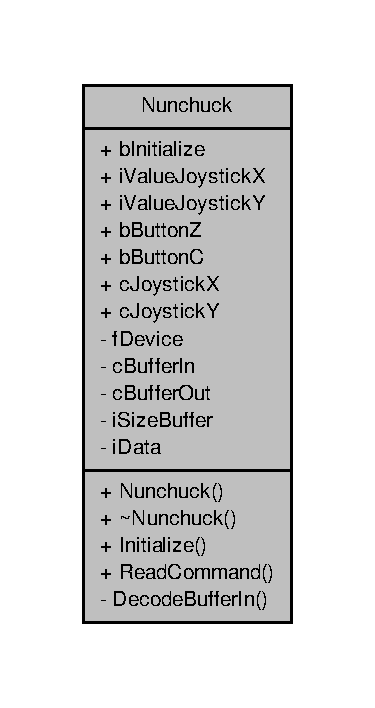
\includegraphics[width=180pt]{classNunchuck__coll__graph}
\end{center}
\end{figure}
\subsection*{Public Member Functions}
\begin{DoxyCompactItemize}
\item 
\hyperlink{classNunchuck_a655b8b1dcb8afcb60b44fcd5ab328407}{Nunchuck} (char c\-Type\-Nunk)
\item 
\hyperlink{classNunchuck_a2ff51de933f8099585f36eee2f280b38}{$\sim$\-Nunchuck} ()
\item 
bool \hyperlink{classNunchuck_aabc3105bbe185edb4521506e5da3dc48}{Initialize} (char c\-Type\-Nunk)
\item 
void \hyperlink{classNunchuck_ade6607a55fda6ae67c90d3d1ee7ce56b}{Read\-Command} ()
\end{DoxyCompactItemize}
\subsection*{Public Attributes}
\begin{DoxyCompactItemize}
\item 
bool \hyperlink{classNunchuck_a3ecbcb3a01a247605b4f0a37b579581d}{b\-Initialize}
\item 
int \hyperlink{classNunchuck_a931870243c74e9df416639c53670b234}{i\-Value\-Joystick\-X}
\item 
int \hyperlink{classNunchuck_a0e084b1760acfc06305bbb339e3c8232}{i\-Value\-Joystick\-Y}
\item 
bool \hyperlink{classNunchuck_a0db1f3d2f58fafda23a5af3936c12598}{b\-Button\-Z}
\item 
bool \hyperlink{classNunchuck_a1d5cac3b603b3060984e3184d795561d}{b\-Button\-C}
\item 
char \hyperlink{classNunchuck_ad9467642b97b8b008ddd137d273a22f8}{c\-Joystick\-X}
\item 
char \hyperlink{classNunchuck_aaf0f299016f5acf686f716518a7ce567}{c\-Joystick\-Y}
\end{DoxyCompactItemize}
\subsection*{Private Member Functions}
\begin{DoxyCompactItemize}
\item 
void \hyperlink{classNunchuck_aac4e5f6da04ee3fb6beada59aefd1612}{Decode\-Buffer\-In} ()
\end{DoxyCompactItemize}
\subsection*{Private Attributes}
\begin{DoxyCompactItemize}
\item 
int \hyperlink{classNunchuck_a61f4874769103ba04e13f75a08442f8e}{f\-Device}
\item 
char \hyperlink{classNunchuck_a1bd7122f88582d12ab2ac5d3c8c7b8f8}{c\-Buffer\-In} \mbox{[}6\mbox{]}
\item 
char \hyperlink{classNunchuck_a4f2eea10fb4eba245c24168ce00429f8}{c\-Buffer\-Out} \mbox{[}2\mbox{]}
\item 
int \hyperlink{classNunchuck_a671e2732508cdd56e51898b79e58d455}{i\-Size\-Buffer}
\item 
int \hyperlink{classNunchuck_a6bf3cbe405e9611658f1a6bbc1cd56b4}{i\-Data} \mbox{[}6\mbox{]}
\end{DoxyCompactItemize}


\subsection{Detailed Description}


Definition at line 31 of file nunchuck.\-h.



\subsection{Constructor \& Destructor Documentation}
\hypertarget{classNunchuck_a655b8b1dcb8afcb60b44fcd5ab328407}{\index{Nunchuck@{Nunchuck}!Nunchuck@{Nunchuck}}
\index{Nunchuck@{Nunchuck}!Nunchuck@{Nunchuck}}
\subsubsection[{Nunchuck}]{\setlength{\rightskip}{0pt plus 5cm}Nunchuck\-::\-Nunchuck (
\begin{DoxyParamCaption}
\item[{char}]{c\-Type\-Nunk}
\end{DoxyParamCaption}
)}}\label{classNunchuck_a655b8b1dcb8afcb60b44fcd5ab328407}


Definition at line 3 of file nunchuck.\-cpp.



References b\-Initialize, Initialize(), and Read\-Command().


\begin{DoxyCode}
\{
    \textcolor{comment}{/*   Initialisation du nunchuck}
\textcolor{comment}{         "bInitialize" est égale à VRAI si l'objet est correctement initialisé 
        */}

    \hyperlink{classNunchuck_a3ecbcb3a01a247605b4f0a37b579581d}{bInitialize} = \hyperlink{classNunchuck_aabc3105bbe185edb4521506e5da3dc48}{Initialize}(cTypeNunk);

    \textcolor{comment}{/*  Lecture des informations commandes  :   Passe "bInitialize" à FAUX en
       cas d'échec   */}
    \textcolor{keywordflow}{if}(\hyperlink{classNunchuck_a3ecbcb3a01a247605b4f0a37b579581d}{bInitialize})\{
        \hyperlink{classNunchuck_ade6607a55fda6ae67c90d3d1ee7ce56b}{ReadCommand}();
    \}
    \textcolor{keywordflow}{else} \{

    \}
\}
\end{DoxyCode}
\hypertarget{classNunchuck_a2ff51de933f8099585f36eee2f280b38}{\index{Nunchuck@{Nunchuck}!$\sim$\-Nunchuck@{$\sim$\-Nunchuck}}
\index{$\sim$\-Nunchuck@{$\sim$\-Nunchuck}!Nunchuck@{Nunchuck}}
\subsubsection[{$\sim$\-Nunchuck}]{\setlength{\rightskip}{0pt plus 5cm}Nunchuck\-::$\sim$\-Nunchuck (
\begin{DoxyParamCaption}
{}
\end{DoxyParamCaption}
)}}\label{classNunchuck_a2ff51de933f8099585f36eee2f280b38}


Definition at line 19 of file nunchuck.\-cpp.



References f\-Device.


\begin{DoxyCode}
\{
    close(\hyperlink{classNunchuck_a61f4874769103ba04e13f75a08442f8e}{fDevice});
\}
\end{DoxyCode}


\subsection{Member Function Documentation}
\hypertarget{classNunchuck_aac4e5f6da04ee3fb6beada59aefd1612}{\index{Nunchuck@{Nunchuck}!Decode\-Buffer\-In@{Decode\-Buffer\-In}}
\index{Decode\-Buffer\-In@{Decode\-Buffer\-In}!Nunchuck@{Nunchuck}}
\subsubsection[{Decode\-Buffer\-In}]{\setlength{\rightskip}{0pt plus 5cm}void Nunchuck\-::\-Decode\-Buffer\-In (
\begin{DoxyParamCaption}
{}
\end{DoxyParamCaption}
)\hspace{0.3cm}{\ttfamily [private]}}}\label{classNunchuck_aac4e5f6da04ee3fb6beada59aefd1612}


Definition at line 128 of file nunchuck.\-cpp.



References b\-Button\-C, b\-Button\-Z, b\-Initialize, c\-Buffer\-In, c\-Joystick\-X, c\-Joystick\-Y, i\-Data, i\-Value\-Joystick\-X, i\-Value\-Joystick\-Y, J\-B\-A\-S, J\-B\-A\-S\-\_\-\-M\-A\-X, J\-C\-E\-N\-T\-R\-E, J\-D\-R\-O\-I\-T\-E, J\-D\-R\-O\-I\-T\-E\-\_\-\-M\-A\-X, J\-G\-A\-U\-C\-H\-E, J\-G\-A\-U\-C\-H\-E\-\_\-\-M\-A\-X, J\-H\-A\-U\-T, and J\-H\-A\-U\-T\-\_\-\-M\-A\-X.



Referenced by Read\-Command().


\begin{DoxyCode}
                              \{

    \textcolor{comment}{/*  Données recu sans cryptage  */}

    \textcolor{keywordflow}{for}(\textcolor{keywordtype}{int} i = 0 ; i < 6 ; i++) \{
        \textcolor{comment}{//cBufferIn[i] ^= 0x17;}
        \hyperlink{classNunchuck_a6bf3cbe405e9611658f1a6bbc1cd56b4}{iData}[i]      = (int)\hyperlink{classNunchuck_a1bd7122f88582d12ab2ac5d3c8c7b8f8}{cBufferIn}[i];
        \textcolor{comment}{//iData[i]     += 0x17;}
    \}


    \textcolor{keywordflow}{if}(\hyperlink{classNunchuck_a3ecbcb3a01a247605b4f0a37b579581d}{bInitialize}) \{

        \textcolor{comment}{//FILE *file = fopen("/tmp/nunchuckLog", "a");}

        \textcolor{comment}{/*  Test Bouttons : Si on appui sur le bouton Z, le bouton C est
       indiqué comme appuyé :}
\textcolor{comment}{         *}
\textcolor{comment}{         *Solution -> on ne test pas le bouton C si Z est appuyé    */}

        \textcolor{keywordflow}{if}(\hyperlink{classNunchuck_a6bf3cbe405e9611658f1a6bbc1cd56b4}{iData}[5] & 0x01) \{                           \textcolor{comment}{//Si Boutton Z
       relaché}

            \hyperlink{classNunchuck_a0db1f3d2f58fafda23a5af3936c12598}{bButtonZ} = \textcolor{keyword}{false};

            \hyperlink{classNunchuck_a6bf3cbe405e9611658f1a6bbc1cd56b4}{iData}[5] >>= 1;

            \textcolor{keywordflow}{if}( \hyperlink{classNunchuck_a6bf3cbe405e9611658f1a6bbc1cd56b4}{iData}[5] & 0x01 ) \{                     \textcolor{comment}{//Si Boutton C
       relaché}
                \hyperlink{classNunchuck_a1d5cac3b603b3060984e3184d795561d}{bButtonC} = \textcolor{keyword}{false};
            \}
            \textcolor{keywordflow}{else} \{                                      \textcolor{comment}{//Si Boutton C appuyé}
                \hyperlink{classNunchuck_a1d5cac3b603b3060984e3184d795561d}{bButtonC} = \textcolor{keyword}{true};
            \}
        \}                                               \textcolor{comment}{//Si Boutton Z appuyé}
        \textcolor{keywordflow}{else} \{
            \hyperlink{classNunchuck_a0db1f3d2f58fafda23a5af3936c12598}{bButtonZ} = \textcolor{keyword}{true};
        \}

        \textcolor{comment}{/*  Test Joystick axe horizontal (X)    */}

        \hyperlink{classNunchuck_a931870243c74e9df416639c53670b234}{iValueJoystickX} = \hyperlink{classNunchuck_a6bf3cbe405e9611658f1a6bbc1cd56b4}{iData}[0];

        \textcolor{keywordflow}{if}(\hyperlink{classNunchuck_a931870243c74e9df416639c53670b234}{iValueJoystickX} > 175) \{    \textcolor{comment}{//Si Joystick à Droite}
            \hyperlink{classNunchuck_ad9467642b97b8b008ddd137d273a22f8}{cJoystickX} = \hyperlink{nunchuck_8h_abb937f82823e628ca09a026777179226}{JDROITE};

            \textcolor{keywordflow}{if}(\hyperlink{classNunchuck_a931870243c74e9df416639c53670b234}{iValueJoystickX} > 225)
                \hyperlink{classNunchuck_ad9467642b97b8b008ddd137d273a22f8}{cJoystickX} = \hyperlink{nunchuck_8h_a13baf3bab74f21c7050fb8029bf5b871}{JDROITE\_MAX};
        \}
        \textcolor{keywordflow}{else} \textcolor{keywordflow}{if}(\hyperlink{classNunchuck_a6bf3cbe405e9611658f1a6bbc1cd56b4}{iData}[0] < 95) \{           \textcolor{comment}{//Si Joystick à Gauche}
            \hyperlink{classNunchuck_ad9467642b97b8b008ddd137d273a22f8}{cJoystickX} = \hyperlink{nunchuck_8h_a2948a7fb931671c2935a67be056ec44d}{JGAUCHE};

            \textcolor{keywordflow}{if}(\hyperlink{classNunchuck_a931870243c74e9df416639c53670b234}{iValueJoystickX} < 50)
                \hyperlink{classNunchuck_ad9467642b97b8b008ddd137d273a22f8}{cJoystickX} = \hyperlink{nunchuck_8h_a19f4efb3793bd7fd7da3a60339dc4631}{JGAUCHE\_MAX};
        \}
        \textcolor{keywordflow}{else} \{                              \textcolor{comment}{//Si Joystick au Centre}
            \hyperlink{classNunchuck_ad9467642b97b8b008ddd137d273a22f8}{cJoystickX} = \hyperlink{nunchuck_8h_ac63506adba6ed764c5061ac249623554}{JCENTRE};
        \}


        \textcolor{comment}{/*  Test Joystick axe vertical (Y)    */}

        \hyperlink{classNunchuck_a0e084b1760acfc06305bbb339e3c8232}{iValueJoystickY} = \hyperlink{classNunchuck_a6bf3cbe405e9611658f1a6bbc1cd56b4}{iData}[1];

        \textcolor{keywordflow}{if}(\hyperlink{classNunchuck_a6bf3cbe405e9611658f1a6bbc1cd56b4}{iData}[1] > 175) \{    \textcolor{comment}{//Si Joystick en Haut}
            \hyperlink{classNunchuck_aaf0f299016f5acf686f716518a7ce567}{cJoystickY} = \hyperlink{nunchuck_8h_a624208e4279eb8508e4d7a4cd1983293}{JHAUT};

            \textcolor{keywordflow}{if}(\hyperlink{classNunchuck_a6bf3cbe405e9611658f1a6bbc1cd56b4}{iData}[1] > 225)
                \hyperlink{classNunchuck_aaf0f299016f5acf686f716518a7ce567}{cJoystickY} = \hyperlink{nunchuck_8h_a69c726c7ddc8415a81ea58834356ed2b}{JHAUT\_MAX};
        \}
        \textcolor{keywordflow}{else} \textcolor{keywordflow}{if}(\hyperlink{classNunchuck_a6bf3cbe405e9611658f1a6bbc1cd56b4}{iData}[1] < 95) \{      \textcolor{comment}{//Si Joystick en Bas}
            \hyperlink{classNunchuck_aaf0f299016f5acf686f716518a7ce567}{cJoystickY} = \hyperlink{nunchuck_8h_ad9a8fe51b03c91dc0256cc7502d450a3}{JBAS};

            \textcolor{keywordflow}{if}(\hyperlink{classNunchuck_a6bf3cbe405e9611658f1a6bbc1cd56b4}{iData}[1] < 50)
                \hyperlink{classNunchuck_aaf0f299016f5acf686f716518a7ce567}{cJoystickY} = \hyperlink{nunchuck_8h_a8bd0c46505c3f0a7d5bc412d8a56d41a}{JBAS\_MAX};
        \}
        \textcolor{keywordflow}{else} \{                         \textcolor{comment}{//Si Joystick au Centre}
            \hyperlink{classNunchuck_aaf0f299016f5acf686f716518a7ce567}{cJoystickY} = \hyperlink{nunchuck_8h_ac63506adba6ed764c5061ac249623554}{JCENTRE};
        \}

        \textcolor{comment}{/*  Accéléromètre}
\textcolor{comment}{            cBufferIn[2] <<= 2;}
\textcolor{comment}{            cBufferIn[2] |= ((cBufferIn[5] >> 2) & 0x03);}
\textcolor{comment}{            printf("X-axis: %d\(\backslash\)n", cBufferIn[2]);}
\textcolor{comment}{}
\textcolor{comment}{            cBufferIn[3] <<= 2;}
\textcolor{comment}{            cBufferIn[3] |= ((cBufferIn[5] >> 4) & 0x03);}
\textcolor{comment}{            printf("Y-axis: %d\(\backslash\)n", cBufferIn[3]);}
\textcolor{comment}{}
\textcolor{comment}{            cBufferIn[4] <<= 2;}
\textcolor{comment}{            cBufferIn[4] |= ((cBufferIn[5] >> 6) & 0x03);}
\textcolor{comment}{            printf("Z-axis: %d\(\backslash\)n", cBufferIn[4]);   */}


        \textcolor{comment}{//fclose(file);}
    \}



\}
\end{DoxyCode}
\hypertarget{classNunchuck_aabc3105bbe185edb4521506e5da3dc48}{\index{Nunchuck@{Nunchuck}!Initialize@{Initialize}}
\index{Initialize@{Initialize}!Nunchuck@{Nunchuck}}
\subsubsection[{Initialize}]{\setlength{\rightskip}{0pt plus 5cm}bool Nunchuck\-::\-Initialize (
\begin{DoxyParamCaption}
\item[{char}]{c\-Type\-Nunk}
\end{DoxyParamCaption}
)}}\label{classNunchuck_aabc3105bbe185edb4521506e5da3dc48}


Definition at line 24 of file nunchuck.\-cpp.



References b\-Button\-C, b\-Button\-Z, c\-Buffer\-Out, c\-Joystick\-X, c\-Joystick\-Y, f\-Device, i\-Size\-Buffer, i\-Value\-Joystick\-X, i\-Value\-Joystick\-Y, and P\-A\-R\-A\-M\-\_\-\-D\-E\-V\-I\-C\-E\-N\-A\-M\-E\-\_\-\-C\-O\-M\-M\-A\-N\-D\-E.



Referenced by Nunchuck(), and Q\-Base\-::\-Q\-Base().


\begin{DoxyCode}
\{
    \textcolor{keywordtype}{int} iAddress\_I2C = 0x52;

    \textcolor{keywordtype}{char} cDeviceName[] = \hyperlink{nunchuck_8h_a0f3e5db0fbc68310b4cdc94e00f10f75}{PARAM\_DEVICENAME\_COMMANDE};

    cDeviceName[\textcolor{keyword}{sizeof}(cDeviceName)-2] = cTypeNunk;

    \textcolor{comment}{/*  Initialisation des variables et  périphériques (Joystick,
       Accéléromètre)   */}

    \hyperlink{classNunchuck_a1d5cac3b603b3060984e3184d795561d}{bButtonC} = \textcolor{keyword}{false};
    \hyperlink{classNunchuck_a0db1f3d2f58fafda23a5af3936c12598}{bButtonZ} = \textcolor{keyword}{false};
    \hyperlink{classNunchuck_ad9467642b97b8b008ddd137d273a22f8}{cJoystickX} = -1;
    \hyperlink{classNunchuck_aaf0f299016f5acf686f716518a7ce567}{cJoystickY} = -1;
    \hyperlink{classNunchuck_a0e084b1760acfc06305bbb339e3c8232}{iValueJoystickY} = -1;
    \hyperlink{classNunchuck_a931870243c74e9df416639c53670b234}{iValueJoystickX} = -1;

    \textcolor{keywordflow}{if} ((\hyperlink{classNunchuck_a61f4874769103ba04e13f75a08442f8e}{fDevice} = open(cDeviceName, O\_RDWR)) < 0) \{
    \textcolor{comment}{/*   Si le périphérique est inéxistant on retourne FAUX   */}
            \textcolor{keywordflow}{return} \textcolor{keyword}{false};
    \}
    \textcolor{keywordflow}{else} \{

    \}

    \textcolor{keywordflow}{if}(ioctl(\hyperlink{classNunchuck_a61f4874769103ba04e13f75a08442f8e}{fDevice}, I2C\_SLAVE, iAddress\_I2C) < 0) \{
    \textcolor{comment}{/*   Si le nunchuck ne répond pas on retourne FAUX   */}
        close(\hyperlink{classNunchuck_a61f4874769103ba04e13f75a08442f8e}{fDevice});
        \textcolor{keywordflow}{return} \textcolor{keyword}{false};
    \}
    \textcolor{keywordflow}{else} \{

    \}

    \textcolor{comment}{/*  Si le nunchuck est reconnue, on l'initialise    */}

    \hyperlink{classNunchuck_a671e2732508cdd56e51898b79e58d455}{iSizeBuffer} = 0;

    \hyperlink{classNunchuck_a4f2eea10fb4eba245c24168ce00429f8}{cBufferOut}[\hyperlink{classNunchuck_a671e2732508cdd56e51898b79e58d455}{iSizeBuffer}++] = 0xF0;
    \hyperlink{classNunchuck_a4f2eea10fb4eba245c24168ce00429f8}{cBufferOut}[\hyperlink{classNunchuck_a671e2732508cdd56e51898b79e58d455}{iSizeBuffer}++] = 0x55;


    \textcolor{keywordflow}{if}(write(\hyperlink{classNunchuck_a61f4874769103ba04e13f75a08442f8e}{fDevice}, \hyperlink{classNunchuck_a4f2eea10fb4eba245c24168ce00429f8}{cBufferOut}, \hyperlink{classNunchuck_a671e2732508cdd56e51898b79e58d455}{iSizeBuffer}) != 
      \hyperlink{classNunchuck_a671e2732508cdd56e51898b79e58d455}{iSizeBuffer}) \{
    \textcolor{comment}{/*   Si il y a erreur d'écriture, on retourne FAUX   */}
        close(\hyperlink{classNunchuck_a61f4874769103ba04e13f75a08442f8e}{fDevice});
        \textcolor{keywordflow}{return} \textcolor{keyword}{false};
    \}
    \textcolor{keywordflow}{else} \{

    \}

    \hyperlink{classNunchuck_a671e2732508cdd56e51898b79e58d455}{iSizeBuffer} = 0;

    \hyperlink{classNunchuck_a4f2eea10fb4eba245c24168ce00429f8}{cBufferOut}[\hyperlink{classNunchuck_a671e2732508cdd56e51898b79e58d455}{iSizeBuffer}++] = 0xFB;
    \hyperlink{classNunchuck_a4f2eea10fb4eba245c24168ce00429f8}{cBufferOut}[\hyperlink{classNunchuck_a671e2732508cdd56e51898b79e58d455}{iSizeBuffer}++] = 0x00;


    \textcolor{keywordflow}{if}(write(\hyperlink{classNunchuck_a61f4874769103ba04e13f75a08442f8e}{fDevice}, \hyperlink{classNunchuck_a4f2eea10fb4eba245c24168ce00429f8}{cBufferOut}, \hyperlink{classNunchuck_a671e2732508cdd56e51898b79e58d455}{iSizeBuffer}) != 
      \hyperlink{classNunchuck_a671e2732508cdd56e51898b79e58d455}{iSizeBuffer}) \{
    \textcolor{comment}{/*   Si il y a erreur d'écriture, on retourne FAUX   */}
        close(\hyperlink{classNunchuck_a61f4874769103ba04e13f75a08442f8e}{fDevice});
        \textcolor{keywordflow}{return} \textcolor{keyword}{false};
    \}
    \textcolor{keywordflow}{else} \{

    \}

    \textcolor{comment}{/*  Nunchuck Initialisé est calibré}
\textcolor{comment}{        On retourne VRAI  */}

    \textcolor{keywordflow}{return} \textcolor{keyword}{true};
\}
\end{DoxyCode}
\hypertarget{classNunchuck_ade6607a55fda6ae67c90d3d1ee7ce56b}{\index{Nunchuck@{Nunchuck}!Read\-Command@{Read\-Command}}
\index{Read\-Command@{Read\-Command}!Nunchuck@{Nunchuck}}
\subsubsection[{Read\-Command}]{\setlength{\rightskip}{0pt plus 5cm}void Nunchuck\-::\-Read\-Command (
\begin{DoxyParamCaption}
{}
\end{DoxyParamCaption}
)}}\label{classNunchuck_ade6607a55fda6ae67c90d3d1ee7ce56b}


Definition at line 96 of file nunchuck.\-cpp.



References b\-Initialize, c\-Buffer\-In, c\-Buffer\-Out, Decode\-Buffer\-In(), f\-Device, and i\-Size\-Buffer.



Referenced by Nunchuck(), and Q\-Base\-::run().


\begin{DoxyCode}
                           \{

    \hyperlink{classNunchuck_a671e2732508cdd56e51898b79e58d455}{iSizeBuffer} = 1;

    \textcolor{comment}{/*  Ordre de lecture des informations des capteurs   */}
    \hyperlink{classNunchuck_a4f2eea10fb4eba245c24168ce00429f8}{cBufferOut}[0] = 0x00;

    \textcolor{keywordflow}{if}(write(\hyperlink{classNunchuck_a61f4874769103ba04e13f75a08442f8e}{fDevice}, \hyperlink{classNunchuck_a4f2eea10fb4eba245c24168ce00429f8}{cBufferOut}, \hyperlink{classNunchuck_a671e2732508cdd56e51898b79e58d455}{iSizeBuffer}) != 
      \hyperlink{classNunchuck_a671e2732508cdd56e51898b79e58d455}{iSizeBuffer}) \{
    \textcolor{comment}{/*   Si il y a erreur d'écriture, demande une réinitialisation   */}
       \hyperlink{classNunchuck_a3ecbcb3a01a247605b4f0a37b579581d}{bInitialize} = \textcolor{keyword}{false};
       close(\hyperlink{classNunchuck_a61f4874769103ba04e13f75a08442f8e}{fDevice});
       \textcolor{keywordflow}{return};
    \}
    \textcolor{keywordflow}{else} \{

    \}

    \hyperlink{classNunchuck_a671e2732508cdd56e51898b79e58d455}{iSizeBuffer} = 6;

    \textcolor{keywordflow}{if}(read(\hyperlink{classNunchuck_a61f4874769103ba04e13f75a08442f8e}{fDevice}, \hyperlink{classNunchuck_a1bd7122f88582d12ab2ac5d3c8c7b8f8}{cBufferIn}, \hyperlink{classNunchuck_a671e2732508cdd56e51898b79e58d455}{iSizeBuffer}) != 
      \hyperlink{classNunchuck_a671e2732508cdd56e51898b79e58d455}{iSizeBuffer}) \{
    \textcolor{comment}{/*   Si il y a erreur de lecture, demande une réinitialisation   */}
       \hyperlink{classNunchuck_a3ecbcb3a01a247605b4f0a37b579581d}{bInitialize} = \textcolor{keyword}{false};
       close(\hyperlink{classNunchuck_a61f4874769103ba04e13f75a08442f8e}{fDevice});
       \textcolor{keywordflow}{return};
    \}
    \textcolor{keywordflow}{else} \{

    \}

    \hyperlink{classNunchuck_aac4e5f6da04ee3fb6beada59aefd1612}{DecodeBufferIn}();
\}
\end{DoxyCode}


\subsection{Member Data Documentation}
\hypertarget{classNunchuck_a1d5cac3b603b3060984e3184d795561d}{\index{Nunchuck@{Nunchuck}!b\-Button\-C@{b\-Button\-C}}
\index{b\-Button\-C@{b\-Button\-C}!Nunchuck@{Nunchuck}}
\subsubsection[{b\-Button\-C}]{\setlength{\rightskip}{0pt plus 5cm}bool Nunchuck\-::b\-Button\-C}}\label{classNunchuck_a1d5cac3b603b3060984e3184d795561d}


Definition at line 49 of file nunchuck.\-h.



Referenced by Decode\-Buffer\-In(), Initialize(), and Q\-Base\-::run().

\hypertarget{classNunchuck_a0db1f3d2f58fafda23a5af3936c12598}{\index{Nunchuck@{Nunchuck}!b\-Button\-Z@{b\-Button\-Z}}
\index{b\-Button\-Z@{b\-Button\-Z}!Nunchuck@{Nunchuck}}
\subsubsection[{b\-Button\-Z}]{\setlength{\rightskip}{0pt plus 5cm}bool Nunchuck\-::b\-Button\-Z}}\label{classNunchuck_a0db1f3d2f58fafda23a5af3936c12598}


Definition at line 48 of file nunchuck.\-h.



Referenced by Decode\-Buffer\-In(), Initialize(), and Q\-Base\-::run().

\hypertarget{classNunchuck_a3ecbcb3a01a247605b4f0a37b579581d}{\index{Nunchuck@{Nunchuck}!b\-Initialize@{b\-Initialize}}
\index{b\-Initialize@{b\-Initialize}!Nunchuck@{Nunchuck}}
\subsubsection[{b\-Initialize}]{\setlength{\rightskip}{0pt plus 5cm}bool Nunchuck\-::b\-Initialize}}\label{classNunchuck_a3ecbcb3a01a247605b4f0a37b579581d}


Definition at line 39 of file nunchuck.\-h.



Referenced by Decode\-Buffer\-In(), Nunchuck(), Q\-Base\-::\-Q\-Base(), Read\-Command(), and Q\-Base\-::run().

\hypertarget{classNunchuck_a1bd7122f88582d12ab2ac5d3c8c7b8f8}{\index{Nunchuck@{Nunchuck}!c\-Buffer\-In@{c\-Buffer\-In}}
\index{c\-Buffer\-In@{c\-Buffer\-In}!Nunchuck@{Nunchuck}}
\subsubsection[{c\-Buffer\-In}]{\setlength{\rightskip}{0pt plus 5cm}char Nunchuck\-::c\-Buffer\-In\mbox{[}6\mbox{]}\hspace{0.3cm}{\ttfamily [private]}}}\label{classNunchuck_a1bd7122f88582d12ab2ac5d3c8c7b8f8}


Definition at line 59 of file nunchuck.\-h.



Referenced by Decode\-Buffer\-In(), and Read\-Command().

\hypertarget{classNunchuck_a4f2eea10fb4eba245c24168ce00429f8}{\index{Nunchuck@{Nunchuck}!c\-Buffer\-Out@{c\-Buffer\-Out}}
\index{c\-Buffer\-Out@{c\-Buffer\-Out}!Nunchuck@{Nunchuck}}
\subsubsection[{c\-Buffer\-Out}]{\setlength{\rightskip}{0pt plus 5cm}char Nunchuck\-::c\-Buffer\-Out\mbox{[}2\mbox{]}\hspace{0.3cm}{\ttfamily [private]}}}\label{classNunchuck_a4f2eea10fb4eba245c24168ce00429f8}


Definition at line 60 of file nunchuck.\-h.



Referenced by Initialize(), and Read\-Command().

\hypertarget{classNunchuck_ad9467642b97b8b008ddd137d273a22f8}{\index{Nunchuck@{Nunchuck}!c\-Joystick\-X@{c\-Joystick\-X}}
\index{c\-Joystick\-X@{c\-Joystick\-X}!Nunchuck@{Nunchuck}}
\subsubsection[{c\-Joystick\-X}]{\setlength{\rightskip}{0pt plus 5cm}char Nunchuck\-::c\-Joystick\-X}}\label{classNunchuck_ad9467642b97b8b008ddd137d273a22f8}


Definition at line 50 of file nunchuck.\-h.



Referenced by Decode\-Buffer\-In(), Initialize(), and Q\-Base\-::run().

\hypertarget{classNunchuck_aaf0f299016f5acf686f716518a7ce567}{\index{Nunchuck@{Nunchuck}!c\-Joystick\-Y@{c\-Joystick\-Y}}
\index{c\-Joystick\-Y@{c\-Joystick\-Y}!Nunchuck@{Nunchuck}}
\subsubsection[{c\-Joystick\-Y}]{\setlength{\rightskip}{0pt plus 5cm}char Nunchuck\-::c\-Joystick\-Y}}\label{classNunchuck_aaf0f299016f5acf686f716518a7ce567}


Definition at line 51 of file nunchuck.\-h.



Referenced by Decode\-Buffer\-In(), Initialize(), and Q\-Base\-::run().

\hypertarget{classNunchuck_a61f4874769103ba04e13f75a08442f8e}{\index{Nunchuck@{Nunchuck}!f\-Device@{f\-Device}}
\index{f\-Device@{f\-Device}!Nunchuck@{Nunchuck}}
\subsubsection[{f\-Device}]{\setlength{\rightskip}{0pt plus 5cm}int Nunchuck\-::f\-Device\hspace{0.3cm}{\ttfamily [private]}}}\label{classNunchuck_a61f4874769103ba04e13f75a08442f8e}


Definition at line 58 of file nunchuck.\-h.



Referenced by Initialize(), Read\-Command(), and $\sim$\-Nunchuck().

\hypertarget{classNunchuck_a6bf3cbe405e9611658f1a6bbc1cd56b4}{\index{Nunchuck@{Nunchuck}!i\-Data@{i\-Data}}
\index{i\-Data@{i\-Data}!Nunchuck@{Nunchuck}}
\subsubsection[{i\-Data}]{\setlength{\rightskip}{0pt plus 5cm}int Nunchuck\-::i\-Data\mbox{[}6\mbox{]}\hspace{0.3cm}{\ttfamily [private]}}}\label{classNunchuck_a6bf3cbe405e9611658f1a6bbc1cd56b4}


Definition at line 64 of file nunchuck.\-h.



Referenced by Decode\-Buffer\-In().

\hypertarget{classNunchuck_a671e2732508cdd56e51898b79e58d455}{\index{Nunchuck@{Nunchuck}!i\-Size\-Buffer@{i\-Size\-Buffer}}
\index{i\-Size\-Buffer@{i\-Size\-Buffer}!Nunchuck@{Nunchuck}}
\subsubsection[{i\-Size\-Buffer}]{\setlength{\rightskip}{0pt plus 5cm}int Nunchuck\-::i\-Size\-Buffer\hspace{0.3cm}{\ttfamily [private]}}}\label{classNunchuck_a671e2732508cdd56e51898b79e58d455}


Definition at line 61 of file nunchuck.\-h.



Referenced by Initialize(), and Read\-Command().

\hypertarget{classNunchuck_a931870243c74e9df416639c53670b234}{\index{Nunchuck@{Nunchuck}!i\-Value\-Joystick\-X@{i\-Value\-Joystick\-X}}
\index{i\-Value\-Joystick\-X@{i\-Value\-Joystick\-X}!Nunchuck@{Nunchuck}}
\subsubsection[{i\-Value\-Joystick\-X}]{\setlength{\rightskip}{0pt plus 5cm}int Nunchuck\-::i\-Value\-Joystick\-X}}\label{classNunchuck_a931870243c74e9df416639c53670b234}


Definition at line 46 of file nunchuck.\-h.



Referenced by Decode\-Buffer\-In(), and Initialize().

\hypertarget{classNunchuck_a0e084b1760acfc06305bbb339e3c8232}{\index{Nunchuck@{Nunchuck}!i\-Value\-Joystick\-Y@{i\-Value\-Joystick\-Y}}
\index{i\-Value\-Joystick\-Y@{i\-Value\-Joystick\-Y}!Nunchuck@{Nunchuck}}
\subsubsection[{i\-Value\-Joystick\-Y}]{\setlength{\rightskip}{0pt plus 5cm}int Nunchuck\-::i\-Value\-Joystick\-Y}}\label{classNunchuck_a0e084b1760acfc06305bbb339e3c8232}


Definition at line 47 of file nunchuck.\-h.



Referenced by Decode\-Buffer\-In(), and Initialize().



The documentation for this class was generated from the following files\-:\begin{DoxyCompactItemize}
\item 
\hyperlink{nunchuck_8h}{nunchuck.\-h}\item 
\hyperlink{nunchuck_8cpp}{nunchuck.\-cpp}\end{DoxyCompactItemize}

\hypertarget{classqAttitudeIndicator}{\section{q\-Attitude\-Indicator Class Reference}
\label{classqAttitudeIndicator}\index{q\-Attitude\-Indicator@{q\-Attitude\-Indicator}}
}


{\ttfamily \#include \char`\"{}qattitudeindicator.\-h\char`\"{}}



Collaboration diagram for q\-Attitude\-Indicator\-:\nopagebreak
\begin{figure}[H]
\begin{center}
\leavevmode
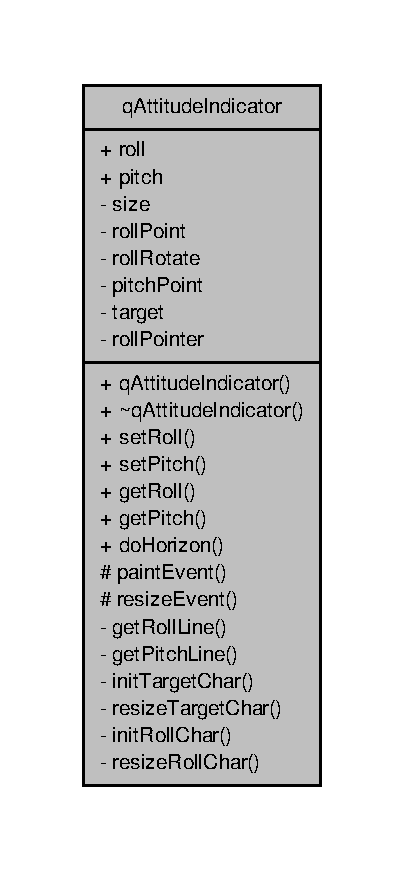
\includegraphics[width=194pt]{classqAttitudeIndicator__coll__graph}
\end{center}
\end{figure}
\subsection*{Public Member Functions}
\begin{DoxyCompactItemize}
\item 
\hyperlink{classqAttitudeIndicator_abe94ed4d04dc448478a7ba19b42790b4}{q\-Attitude\-Indicator} (Q\-Widget $\ast$parent=0)
\item 
\hyperlink{classqAttitudeIndicator_a94754ebda94552125ff33481abe5a0ac}{$\sim$q\-Attitude\-Indicator} ()
\item 
void \hyperlink{classqAttitudeIndicator_a68de255908b787293310a088ef47c49b}{set\-Roll} (qreal val)
\item 
void \hyperlink{classqAttitudeIndicator_a5d8bcc03d0ba08c1494b0a32f56de91c}{set\-Pitch} (qreal val)
\item 
qreal \hyperlink{classqAttitudeIndicator_a6073499d7c349663f04dfef0b3788087}{get\-Roll} ()
\item 
qreal \hyperlink{classqAttitudeIndicator_a73dd028c85bba14faaca24b321b077f8}{get\-Pitch} ()
\item 
void \hyperlink{classqAttitudeIndicator_a7d4e7b19bc493de63a91b0e0480c24e2}{do\-Horizon} ()
\end{DoxyCompactItemize}
\subsection*{Public Attributes}
\begin{DoxyCompactItemize}
\item 
qreal \hyperlink{classqAttitudeIndicator_a10c98e2fd9195050cb305f4b12bf75bb}{roll}
\item 
qreal \hyperlink{classqAttitudeIndicator_ae0df6492b15cc2d3f51c3de0e6dd08bd}{pitch}
\end{DoxyCompactItemize}
\subsection*{Protected Member Functions}
\begin{DoxyCompactItemize}
\item 
void \hyperlink{classqAttitudeIndicator_ab78d82e32c6f34dd246ef0deeda82400}{paint\-Event} (Q\-Paint\-Event $\ast$event)
\item 
void \hyperlink{classqAttitudeIndicator_aa37745feddf31f9ce553156ce51732bd}{resize\-Event} (Q\-Resize\-Event $\ast$event)
\end{DoxyCompactItemize}
\subsection*{Private Member Functions}
\begin{DoxyCompactItemize}
\item 
void \hyperlink{classqAttitudeIndicator_aaeaa7be50092cbfbf9b666ef5bc9aa4a}{get\-Roll\-Line} (\hyperlink{qattitudeindicator_8h_a343e47e8a321f67b38cb4522cb218c94}{E\-N\-\_\-\-T\-Y\-P\-E\-S\-\_\-\-A\-T\-T\-I\-T\-U\-D\-E} type, Q\-Point $\ast$p\-From, Q\-Point $\ast$p\-To)
\item 
void \hyperlink{classqAttitudeIndicator_a39c3505cf7817552213bf03c22b12bf7}{get\-Pitch\-Line} (\hyperlink{qattitudeindicator_8h_a343e47e8a321f67b38cb4522cb218c94}{E\-N\-\_\-\-T\-Y\-P\-E\-S\-\_\-\-A\-T\-T\-I\-T\-U\-D\-E} type, quint32 index, Q\-Point $\ast$p\-From, Q\-Point $\ast$p\-To)
\item 
void \hyperlink{classqAttitudeIndicator_a538e6a904f2a6521e21946541c23f596}{init\-Target\-Char} ()
\item 
void \hyperlink{classqAttitudeIndicator_a7589132ed175b095b8867881e99d26ab}{resize\-Target\-Char} ()
\item 
void \hyperlink{classqAttitudeIndicator_a4d477951cd83bf863eca1a395b092727}{init\-Roll\-Char} ()
\item 
void \hyperlink{classqAttitudeIndicator_a4367f3d4ba77c4dafcbbb99d23f00b58}{resize\-Roll\-Char} ()
\end{DoxyCompactItemize}
\subsection*{Private Attributes}
\begin{DoxyCompactItemize}
\item 
int \hyperlink{classqAttitudeIndicator_a0d7a73e4ee536cda1a005f626ef3935f}{size}
\item 
Q\-Point \hyperlink{classqAttitudeIndicator_a739d71cc4dfba5d2fbb23186372c4fd4}{roll\-Point} \mbox{[}\hyperlink{qattitudeindicator_8h_a533fb9cffe544953a1e34ef3ca40cd9aae68d533445c770721902ff44425e6cda}{numb\-Roll\-Line}\mbox{]}\mbox{[}2\mbox{]}
\item 
qreal \hyperlink{classqAttitudeIndicator_afa3060f26300228565f05c0200d553c2}{roll\-Rotate} \mbox{[}\hyperlink{qattitudeindicator_8h_a533fb9cffe544953a1e34ef3ca40cd9aae68d533445c770721902ff44425e6cda}{numb\-Roll\-Line}\mbox{]}
\item 
Q\-Point \hyperlink{classqAttitudeIndicator_a715b6a95898985f0f52ec6bf18010c9e}{pitch\-Point} \mbox{[}\hyperlink{qattitudeindicator_8h_a533fb9cffe544953a1e34ef3ca40cd9aaf86b1d616737ab90eedf9d904603bbc7}{numb\-Pitch\-Line}\mbox{]}\mbox{[}2\mbox{]}
\item 
Q\-Vector$<$ Q\-Line $>$ \hyperlink{classqAttitudeIndicator_a7f5a24dd1bf00a9e81d2aeb0ac83359e}{target}
\item 
Q\-Vector$<$ Q\-Line $>$ \hyperlink{classqAttitudeIndicator_ac5ace954b2f7b2d88aeae586a1246c30}{roll\-Pointer}
\end{DoxyCompactItemize}


\subsection{Detailed Description}


Definition at line 23 of file qattitudeindicator.\-h.



\subsection{Constructor \& Destructor Documentation}
\hypertarget{classqAttitudeIndicator_abe94ed4d04dc448478a7ba19b42790b4}{\index{q\-Attitude\-Indicator@{q\-Attitude\-Indicator}!q\-Attitude\-Indicator@{q\-Attitude\-Indicator}}
\index{q\-Attitude\-Indicator@{q\-Attitude\-Indicator}!qAttitudeIndicator@{q\-Attitude\-Indicator}}
\subsubsection[{q\-Attitude\-Indicator}]{\setlength{\rightskip}{0pt plus 5cm}q\-Attitude\-Indicator\-::q\-Attitude\-Indicator (
\begin{DoxyParamCaption}
\item[{Q\-Widget $\ast$}]{parent = {\ttfamily 0}}
\end{DoxyParamCaption}
)}}\label{classqAttitudeIndicator_abe94ed4d04dc448478a7ba19b42790b4}


Definition at line 17 of file qattitudeindicator.\-cpp.



References defaults\-Roll\-Rotate, defaults\-Type\-Pitch, defaults\-Type\-Roll, get\-Pitch\-Line(), get\-Roll\-Line(), init\-Roll\-Char(), init\-Target\-Char(), numb\-Pitch\-Line, numb\-Roll\-Line, pitch, pitch\-Point, roll, roll\-Point, roll\-Rotate, size, size\-Max, and size\-Min.


\begin{DoxyCode}
    : QWidget(parent)
\{
    \textcolor{comment}{//QTimer *timer = new QTimer(this);}
    \textcolor{comment}{//connect(timer, SIGNAL(timeout()), this, SLOT(update()));}
    \textcolor{comment}{//connect(timer, SIGNAL(timeout()), this, SLOT(nunchuckEvent()));}
    \textcolor{comment}{//timer->start(50);}
    \textcolor{comment}{//startTimer(50);}

    \hyperlink{classqAttitudeIndicator_a0d7a73e4ee536cda1a005f626ef3935f}{size} = \hyperlink{qattitudeindicator_8h_a533fb9cffe544953a1e34ef3ca40cd9aa467c2cfbbeb81431d3520b2a334cbec1}{sizeMin};
    setMinimumSize(\hyperlink{qattitudeindicator_8h_a533fb9cffe544953a1e34ef3ca40cd9aa467c2cfbbeb81431d3520b2a334cbec1}{sizeMin},\hyperlink{qattitudeindicator_8h_a533fb9cffe544953a1e34ef3ca40cd9aa467c2cfbbeb81431d3520b2a334cbec1}{sizeMin});
    setMaximumSize(\hyperlink{qattitudeindicator_8h_a533fb9cffe544953a1e34ef3ca40cd9aa7c4896a6b7e0383b6dc1e1186a186c09}{sizeMax},\hyperlink{qattitudeindicator_8h_a533fb9cffe544953a1e34ef3ca40cd9aa7c4896a6b7e0383b6dc1e1186a186c09}{sizeMax});
    resize(\hyperlink{classqAttitudeIndicator_a0d7a73e4ee536cda1a005f626ef3935f}{size}, \hyperlink{classqAttitudeIndicator_a0d7a73e4ee536cda1a005f626ef3935f}{size});

    \textcolor{comment}{// from 0 degrees;}
    \textcolor{keywordflow}{for}(\textcolor{keywordtype}{int} i=0;i < \hyperlink{qattitudeindicator_8h_a533fb9cffe544953a1e34ef3ca40cd9aae68d533445c770721902ff44425e6cda}{numbRollLine};i++)
    \{
        \hyperlink{classqAttitudeIndicator_afa3060f26300228565f05c0200d553c2}{rollRotate}[i] = \hyperlink{qattitudeindicator_8cpp_a2f4f279d4d5470569f9b4d6db0e913c3}{defaultsRollRotate}[i];
        \hyperlink{classqAttitudeIndicator_aaeaa7be50092cbfbf9b666ef5bc9aa4a}{getRollLine}(\hyperlink{qattitudeindicator_8cpp_a3e866b9c9b8bde50fd68030b49604a15}{defaultsTypeRoll}[i],&\hyperlink{classqAttitudeIndicator_a739d71cc4dfba5d2fbb23186372c4fd4}{rollPoint}
      [i][0],&\hyperlink{classqAttitudeIndicator_a739d71cc4dfba5d2fbb23186372c4fd4}{rollPoint}[i][1]);
    \}
    \textcolor{keywordflow}{for}(\textcolor{keywordtype}{int} i=0;i< \hyperlink{qattitudeindicator_8h_a533fb9cffe544953a1e34ef3ca40cd9aaf86b1d616737ab90eedf9d904603bbc7}{numbPitchLine};i++)
        \hyperlink{classqAttitudeIndicator_a39c3505cf7817552213bf03c22b12bf7}{getPitchLine}(\hyperlink{qattitudeindicator_8cpp_aeb622d2485fb495e7b9864ca595af136}{defaultsTypePitch}[i],i,&
      \hyperlink{classqAttitudeIndicator_a715b6a95898985f0f52ec6bf18010c9e}{pitchPoint}[i][0],&\hyperlink{classqAttitudeIndicator_a715b6a95898985f0f52ec6bf18010c9e}{pitchPoint}[i][1]);

    \hyperlink{classqAttitudeIndicator_a538e6a904f2a6521e21946541c23f596}{initTargetChar}();
    \hyperlink{classqAttitudeIndicator_a4d477951cd83bf863eca1a395b092727}{initRollChar}();
    \hyperlink{classqAttitudeIndicator_a10c98e2fd9195050cb305f4b12bf75bb}{roll} = 0.0;
    \hyperlink{classqAttitudeIndicator_ae0df6492b15cc2d3f51c3de0e6dd08bd}{pitch} = 0.0;

    \textcolor{comment}{//wiiTest = new Nunchuck(PARAM\_DRONE);}
\}
\end{DoxyCode}
\hypertarget{classqAttitudeIndicator_a94754ebda94552125ff33481abe5a0ac}{\index{q\-Attitude\-Indicator@{q\-Attitude\-Indicator}!$\sim$q\-Attitude\-Indicator@{$\sim$q\-Attitude\-Indicator}}
\index{$\sim$q\-Attitude\-Indicator@{$\sim$q\-Attitude\-Indicator}!qAttitudeIndicator@{q\-Attitude\-Indicator}}
\subsubsection[{$\sim$q\-Attitude\-Indicator}]{\setlength{\rightskip}{0pt plus 5cm}q\-Attitude\-Indicator\-::$\sim$q\-Attitude\-Indicator (
\begin{DoxyParamCaption}
{}
\end{DoxyParamCaption}
)}}\label{classqAttitudeIndicator_a94754ebda94552125ff33481abe5a0ac}


Definition at line 48 of file qattitudeindicator.\-cpp.


\begin{DoxyCode}
\{
    \textcolor{comment}{//delete wiiTest;}
\}
\end{DoxyCode}


\subsection{Member Function Documentation}
\hypertarget{classqAttitudeIndicator_a7d4e7b19bc493de63a91b0e0480c24e2}{\index{q\-Attitude\-Indicator@{q\-Attitude\-Indicator}!do\-Horizon@{do\-Horizon}}
\index{do\-Horizon@{do\-Horizon}!qAttitudeIndicator@{q\-Attitude\-Indicator}}
\subsubsection[{do\-Horizon}]{\setlength{\rightskip}{0pt plus 5cm}void q\-Attitude\-Indicator\-::do\-Horizon (
\begin{DoxyParamCaption}
{}
\end{DoxyParamCaption}
)}}\label{classqAttitudeIndicator_a7d4e7b19bc493de63a91b0e0480c24e2}


Definition at line 121 of file qattitudeindicator.\-cpp.



Referenced by Q\-Th\-\_\-\-Base\-::run(), and Q\-Base\-::run().


\begin{DoxyCode}
\{
    update();
\}
\end{DoxyCode}
\hypertarget{classqAttitudeIndicator_a73dd028c85bba14faaca24b321b077f8}{\index{q\-Attitude\-Indicator@{q\-Attitude\-Indicator}!get\-Pitch@{get\-Pitch}}
\index{get\-Pitch@{get\-Pitch}!qAttitudeIndicator@{q\-Attitude\-Indicator}}
\subsubsection[{get\-Pitch}]{\setlength{\rightskip}{0pt plus 5cm}qreal q\-Attitude\-Indicator\-::get\-Pitch (
\begin{DoxyParamCaption}
{}
\end{DoxyParamCaption}
)\hspace{0.3cm}{\ttfamily [inline]}}}\label{classqAttitudeIndicator_a73dd028c85bba14faaca24b321b077f8}


Definition at line 33 of file qattitudeindicator.\-h.



References pitch.


\begin{DoxyCode}
\{\textcolor{keywordflow}{return} \hyperlink{classqAttitudeIndicator_ae0df6492b15cc2d3f51c3de0e6dd08bd}{pitch};\}
\end{DoxyCode}
\hypertarget{classqAttitudeIndicator_a39c3505cf7817552213bf03c22b12bf7}{\index{q\-Attitude\-Indicator@{q\-Attitude\-Indicator}!get\-Pitch\-Line@{get\-Pitch\-Line}}
\index{get\-Pitch\-Line@{get\-Pitch\-Line}!qAttitudeIndicator@{q\-Attitude\-Indicator}}
\subsubsection[{get\-Pitch\-Line}]{\setlength{\rightskip}{0pt plus 5cm}void q\-Attitude\-Indicator\-::get\-Pitch\-Line (
\begin{DoxyParamCaption}
\item[{{\bf E\-N\-\_\-\-T\-Y\-P\-E\-S\-\_\-\-A\-T\-T\-I\-T\-U\-D\-E}}]{type, }
\item[{quint32}]{index, }
\item[{Q\-Point $\ast$}]{p\-From, }
\item[{Q\-Point $\ast$}]{p\-To}
\end{DoxyParamCaption}
)\hspace{0.3cm}{\ttfamily [private]}}}\label{classqAttitudeIndicator_a39c3505cf7817552213bf03c22b12bf7}


Definition at line 98 of file qattitudeindicator.\-cpp.



References size, and small\-Pitch\-Line.



Referenced by q\-Attitude\-Indicator(), and resize\-Event().


\begin{DoxyCode}
\{
    \textcolor{keywordtype}{int} x,y;
    \textcolor{keywordflow}{if}(index>=4) index++;
    y = \hyperlink{classqAttitudeIndicator_a0d7a73e4ee536cda1a005f626ef3935f}{size}*(0.25-index*0.0625);
    x = (type==\hyperlink{qattitudeindicator_8h_a9e6157b3f1ec4c2db1f8a664f6347784a27d8d9b85932b52acefebc1edaebac45}{smallPitchLine})? (3*\hyperlink{classqAttitudeIndicator_a0d7a73e4ee536cda1a005f626ef3935f}{size}/32):(5*\hyperlink{classqAttitudeIndicator_a0d7a73e4ee536cda1a005f626ef3935f}{size}/32);
    pFrom->setX(-x);
    pFrom->setY(y);
    pTo->setX(x);
    pTo->setY(y);
\}
\end{DoxyCode}
\hypertarget{classqAttitudeIndicator_a6073499d7c349663f04dfef0b3788087}{\index{q\-Attitude\-Indicator@{q\-Attitude\-Indicator}!get\-Roll@{get\-Roll}}
\index{get\-Roll@{get\-Roll}!qAttitudeIndicator@{q\-Attitude\-Indicator}}
\subsubsection[{get\-Roll}]{\setlength{\rightskip}{0pt plus 5cm}qreal q\-Attitude\-Indicator\-::get\-Roll (
\begin{DoxyParamCaption}
{}
\end{DoxyParamCaption}
)\hspace{0.3cm}{\ttfamily [inline]}}}\label{classqAttitudeIndicator_a6073499d7c349663f04dfef0b3788087}


Definition at line 32 of file qattitudeindicator.\-h.



References roll.


\begin{DoxyCode}
\{\textcolor{keywordflow}{return} \hyperlink{classqAttitudeIndicator_a10c98e2fd9195050cb305f4b12bf75bb}{roll};\}
\end{DoxyCode}
\hypertarget{classqAttitudeIndicator_aaeaa7be50092cbfbf9b666ef5bc9aa4a}{\index{q\-Attitude\-Indicator@{q\-Attitude\-Indicator}!get\-Roll\-Line@{get\-Roll\-Line}}
\index{get\-Roll\-Line@{get\-Roll\-Line}!qAttitudeIndicator@{q\-Attitude\-Indicator}}
\subsubsection[{get\-Roll\-Line}]{\setlength{\rightskip}{0pt plus 5cm}void q\-Attitude\-Indicator\-::get\-Roll\-Line (
\begin{DoxyParamCaption}
\item[{{\bf E\-N\-\_\-\-T\-Y\-P\-E\-S\-\_\-\-A\-T\-T\-I\-T\-U\-D\-E}}]{type, }
\item[{Q\-Point $\ast$}]{p\-From, }
\item[{Q\-Point $\ast$}]{p\-To}
\end{DoxyParamCaption}
)\hspace{0.3cm}{\ttfamily [private]}}}\label{classqAttitudeIndicator_aaeaa7be50092cbfbf9b666ef5bc9aa4a}


Definition at line 89 of file qattitudeindicator.\-cpp.



References size, and small\-Roll\-Line.



Referenced by q\-Attitude\-Indicator(), and resize\-Event().


\begin{DoxyCode}
\{
    quint8 ofs = (type == \hyperlink{qattitudeindicator_8h_a9e6157b3f1ec4c2db1f8a664f6347784a24e88cb96dabfbd43afd71b24529147a}{smallRollLine})? (\hyperlink{classqAttitudeIndicator_a0d7a73e4ee536cda1a005f626ef3935f}{size}/40) : (\hyperlink{classqAttitudeIndicator_a0d7a73e4ee536cda1a005f626ef3935f}{size}
      /20) ;
    pFrom->setY(\hyperlink{classqAttitudeIndicator_a0d7a73e4ee536cda1a005f626ef3935f}{size}/2-ofs);
    pFrom->setX(0);
    pTo->setY(\hyperlink{classqAttitudeIndicator_a0d7a73e4ee536cda1a005f626ef3935f}{size}/2);
    pTo->setX(0);
\}
\end{DoxyCode}
\hypertarget{classqAttitudeIndicator_a4d477951cd83bf863eca1a395b092727}{\index{q\-Attitude\-Indicator@{q\-Attitude\-Indicator}!init\-Roll\-Char@{init\-Roll\-Char}}
\index{init\-Roll\-Char@{init\-Roll\-Char}!qAttitudeIndicator@{q\-Attitude\-Indicator}}
\subsubsection[{init\-Roll\-Char}]{\setlength{\rightskip}{0pt plus 5cm}void q\-Attitude\-Indicator\-::init\-Roll\-Char (
\begin{DoxyParamCaption}
{}
\end{DoxyParamCaption}
)\hspace{0.3cm}{\ttfamily [private]}}}\label{classqAttitudeIndicator_a4d477951cd83bf863eca1a395b092727}


Definition at line 72 of file qattitudeindicator.\-cpp.



References size, and target.



Referenced by q\-Attitude\-Indicator(), and resize\-Roll\-Char().


\begin{DoxyCode}
\{
    QLine line;
    line.setLine(-\hyperlink{classqAttitudeIndicator_a0d7a73e4ee536cda1a005f626ef3935f}{size}/32,14*\hyperlink{classqAttitudeIndicator_a0d7a73e4ee536cda1a005f626ef3935f}{size}/32,0,15*\hyperlink{classqAttitudeIndicator_a0d7a73e4ee536cda1a005f626ef3935f}{size}/32);
    \hyperlink{classqAttitudeIndicator_a7f5a24dd1bf00a9e81d2aeb0ac83359e}{target}.append(line);
    line.setLine(0,15*\hyperlink{classqAttitudeIndicator_a0d7a73e4ee536cda1a005f626ef3935f}{size}/32,\hyperlink{classqAttitudeIndicator_a0d7a73e4ee536cda1a005f626ef3935f}{size}/32,14*\hyperlink{classqAttitudeIndicator_a0d7a73e4ee536cda1a005f626ef3935f}{size}/32);
    \hyperlink{classqAttitudeIndicator_a7f5a24dd1bf00a9e81d2aeb0ac83359e}{target}.append(line);
    line.setLine(\hyperlink{classqAttitudeIndicator_a0d7a73e4ee536cda1a005f626ef3935f}{size}/32,14*\hyperlink{classqAttitudeIndicator_a0d7a73e4ee536cda1a005f626ef3935f}{size}/32,-\hyperlink{classqAttitudeIndicator_a0d7a73e4ee536cda1a005f626ef3935f}{size}/32,14*\hyperlink{classqAttitudeIndicator_a0d7a73e4ee536cda1a005f626ef3935f}{size}/32);
    \hyperlink{classqAttitudeIndicator_a7f5a24dd1bf00a9e81d2aeb0ac83359e}{target}.append(line);
\}
\end{DoxyCode}
\hypertarget{classqAttitudeIndicator_a538e6a904f2a6521e21946541c23f596}{\index{q\-Attitude\-Indicator@{q\-Attitude\-Indicator}!init\-Target\-Char@{init\-Target\-Char}}
\index{init\-Target\-Char@{init\-Target\-Char}!qAttitudeIndicator@{q\-Attitude\-Indicator}}
\subsubsection[{init\-Target\-Char}]{\setlength{\rightskip}{0pt plus 5cm}void q\-Attitude\-Indicator\-::init\-Target\-Char (
\begin{DoxyParamCaption}
{}
\end{DoxyParamCaption}
)\hspace{0.3cm}{\ttfamily [private]}}}\label{classqAttitudeIndicator_a538e6a904f2a6521e21946541c23f596}


Definition at line 53 of file qattitudeindicator.\-cpp.



References size, and target.



Referenced by q\-Attitude\-Indicator(), and resize\-Target\-Char().


\begin{DoxyCode}
\{
    QLine line;
    line.setLine(-\hyperlink{classqAttitudeIndicator_a0d7a73e4ee536cda1a005f626ef3935f}{size}/4,0,-\hyperlink{classqAttitudeIndicator_a0d7a73e4ee536cda1a005f626ef3935f}{size}/16,0);
    \hyperlink{classqAttitudeIndicator_a7f5a24dd1bf00a9e81d2aeb0ac83359e}{target}.append(line);
    line.setLine(-\hyperlink{classqAttitudeIndicator_a0d7a73e4ee536cda1a005f626ef3935f}{size}/16,0,0,-\hyperlink{classqAttitudeIndicator_a0d7a73e4ee536cda1a005f626ef3935f}{size}/32);
    \hyperlink{classqAttitudeIndicator_a7f5a24dd1bf00a9e81d2aeb0ac83359e}{target}.append(line);
    line.setLine(0,-\hyperlink{classqAttitudeIndicator_a0d7a73e4ee536cda1a005f626ef3935f}{size}/32,\hyperlink{classqAttitudeIndicator_a0d7a73e4ee536cda1a005f626ef3935f}{size}/16,0);
    \hyperlink{classqAttitudeIndicator_a7f5a24dd1bf00a9e81d2aeb0ac83359e}{target}.append(line);
    line.setLine(\hyperlink{classqAttitudeIndicator_a0d7a73e4ee536cda1a005f626ef3935f}{size}/16,0,\hyperlink{classqAttitudeIndicator_a0d7a73e4ee536cda1a005f626ef3935f}{size}/4,0);
    \hyperlink{classqAttitudeIndicator_a7f5a24dd1bf00a9e81d2aeb0ac83359e}{target}.append(line);
\}
\end{DoxyCode}
\hypertarget{classqAttitudeIndicator_ab78d82e32c6f34dd246ef0deeda82400}{\index{q\-Attitude\-Indicator@{q\-Attitude\-Indicator}!paint\-Event@{paint\-Event}}
\index{paint\-Event@{paint\-Event}!qAttitudeIndicator@{q\-Attitude\-Indicator}}
\subsubsection[{paint\-Event}]{\setlength{\rightskip}{0pt plus 5cm}void q\-Attitude\-Indicator\-::paint\-Event (
\begin{DoxyParamCaption}
\item[{Q\-Paint\-Event $\ast$}]{event}
\end{DoxyParamCaption}
)\hspace{0.3cm}{\ttfamily [protected]}}}\label{classqAttitudeIndicator_ab78d82e32c6f34dd246ef0deeda82400}


Definition at line 126 of file qattitudeindicator.\-cpp.



References numb\-Pitch\-Line, numb\-Roll\-Line, pitch, pitch\-Point, roll, roll\-Point, roll\-Pointer, roll\-Rotate, size, and target.


\begin{DoxyCode}
\{
    QPainter painter(\textcolor{keyword}{this});
    QPoint center(0,0);
    QPen whitePen(Qt::white);
    QPen blackPen(Qt::black);
    QBrush bgSky(QColor(48,172,220));
    QBrush bgGround(QColor(247,168,21));
    whitePen.setWidth(2);
    blackPen.setWidth(1);
    painter.setRenderHint(QPainter::Antialiasing);
    painter.translate(width() / 2, height() / 2);
    \textcolor{keywordtype}{int} side = qMin(width(), height());
    painter.scale(side / (qreal)(\hyperlink{classqAttitudeIndicator_a0d7a73e4ee536cda1a005f626ef3935f}{size}), side / (qreal)(\hyperlink{classqAttitudeIndicator_a0d7a73e4ee536cda1a005f626ef3935f}{size}));
    painter.setPen(blackPen);
    painter.rotate(\hyperlink{classqAttitudeIndicator_a10c98e2fd9195050cb305f4b12bf75bb}{roll});
    painter.setBrush(bgSky);

    \textcolor{keywordtype}{int} y = 0.25*\hyperlink{classqAttitudeIndicator_a0d7a73e4ee536cda1a005f626ef3935f}{size}*\hyperlink{classqAttitudeIndicator_ae0df6492b15cc2d3f51c3de0e6dd08bd}{pitch}/20.;

    \textcolor{keywordtype}{int} x = sqrt(\hyperlink{classqAttitudeIndicator_a0d7a73e4ee536cda1a005f626ef3935f}{size}*\hyperlink{classqAttitudeIndicator_a0d7a73e4ee536cda1a005f626ef3935f}{size}/4 - y*y);
    qreal gr = atan((\textcolor{keywordtype}{double})(y)/x);
    gr = gr * 180./3.1415926;
    painter.drawChord(-side/2,-side/2,side,side,gr*16,(180-2*gr)*16);
    painter.setBrush(bgGround);
    painter.drawChord(-side/2,-side/2,side,side,gr*16,-(180+2*gr)*16);
    painter.setPen(whitePen);

    painter.drawLine(-x,-y,x,-y);
    painter.setPen(blackPen);
    painter.rotate(-180.);
    \textcolor{keywordflow}{for}(\textcolor{keywordtype}{int} i=0;i<\hyperlink{qattitudeindicator_8h_a533fb9cffe544953a1e34ef3ca40cd9aae68d533445c770721902ff44425e6cda}{numbRollLine};i++)
    \{
        painter.rotate(\hyperlink{classqAttitudeIndicator_afa3060f26300228565f05c0200d553c2}{rollRotate}[i]);
        painter.drawLine(\hyperlink{classqAttitudeIndicator_a739d71cc4dfba5d2fbb23186372c4fd4}{rollPoint}[i][0],\hyperlink{classqAttitudeIndicator_a739d71cc4dfba5d2fbb23186372c4fd4}{rollPoint}[i][1]);
    \}
    whitePen.setWidth(1);
    painter.setPen(whitePen);
    painter.rotate(-90.);
    \textcolor{keywordflow}{for}(\textcolor{keywordtype}{int} i=0;i<\hyperlink{qattitudeindicator_8h_a533fb9cffe544953a1e34ef3ca40cd9aaf86b1d616737ab90eedf9d904603bbc7}{numbPitchLine};i++)
    \{
        painter.drawLine(\hyperlink{classqAttitudeIndicator_a715b6a95898985f0f52ec6bf18010c9e}{pitchPoint}[i][0],\hyperlink{classqAttitudeIndicator_a715b6a95898985f0f52ec6bf18010c9e}{pitchPoint}[i][1])
      ;
    \}
    painter.rotate(-\hyperlink{classqAttitudeIndicator_a10c98e2fd9195050cb305f4b12bf75bb}{roll});
    blackPen.setWidth(3);
    painter.setPen(blackPen);
    painter.drawLines(\hyperlink{classqAttitudeIndicator_a7f5a24dd1bf00a9e81d2aeb0ac83359e}{target});
    painter.drawLines(\hyperlink{classqAttitudeIndicator_ac5ace954b2f7b2d88aeae586a1246c30}{rollPointer});
\}
\end{DoxyCode}
\hypertarget{classqAttitudeIndicator_aa37745feddf31f9ce553156ce51732bd}{\index{q\-Attitude\-Indicator@{q\-Attitude\-Indicator}!resize\-Event@{resize\-Event}}
\index{resize\-Event@{resize\-Event}!qAttitudeIndicator@{q\-Attitude\-Indicator}}
\subsubsection[{resize\-Event}]{\setlength{\rightskip}{0pt plus 5cm}void q\-Attitude\-Indicator\-::resize\-Event (
\begin{DoxyParamCaption}
\item[{Q\-Resize\-Event $\ast$}]{event}
\end{DoxyParamCaption}
)\hspace{0.3cm}{\ttfamily [protected]}}}\label{classqAttitudeIndicator_aa37745feddf31f9ce553156ce51732bd}


Definition at line 110 of file qattitudeindicator.\-cpp.



References defaults\-Type\-Pitch, defaults\-Type\-Roll, get\-Pitch\-Line(), get\-Roll\-Line(), numb\-Pitch\-Line, numb\-Roll\-Line, pitch\-Point, resize\-Roll\-Char(), resize\-Target\-Char(), roll\-Point, and size.


\begin{DoxyCode}
\{
    \hyperlink{classqAttitudeIndicator_a0d7a73e4ee536cda1a005f626ef3935f}{size} = qMin(width(),height());
    \textcolor{keywordflow}{for}(\textcolor{keywordtype}{int} i=0;i < \hyperlink{qattitudeindicator_8h_a533fb9cffe544953a1e34ef3ca40cd9aae68d533445c770721902ff44425e6cda}{numbRollLine};i++)
        \hyperlink{classqAttitudeIndicator_aaeaa7be50092cbfbf9b666ef5bc9aa4a}{getRollLine}(\hyperlink{qattitudeindicator_8cpp_a3e866b9c9b8bde50fd68030b49604a15}{defaultsTypeRoll}[i],&\hyperlink{classqAttitudeIndicator_a739d71cc4dfba5d2fbb23186372c4fd4}{rollPoint}
      [i][0],&\hyperlink{classqAttitudeIndicator_a739d71cc4dfba5d2fbb23186372c4fd4}{rollPoint}[i][1]);
    \textcolor{keywordflow}{for}(\textcolor{keywordtype}{int} i=0;i< \hyperlink{qattitudeindicator_8h_a533fb9cffe544953a1e34ef3ca40cd9aaf86b1d616737ab90eedf9d904603bbc7}{numbPitchLine};i++)
        \hyperlink{classqAttitudeIndicator_a39c3505cf7817552213bf03c22b12bf7}{getPitchLine}(\hyperlink{qattitudeindicator_8cpp_aeb622d2485fb495e7b9864ca595af136}{defaultsTypePitch}[i],i,&
      \hyperlink{classqAttitudeIndicator_a715b6a95898985f0f52ec6bf18010c9e}{pitchPoint}[i][0],&\hyperlink{classqAttitudeIndicator_a715b6a95898985f0f52ec6bf18010c9e}{pitchPoint}[i][1]);
    \hyperlink{classqAttitudeIndicator_a7589132ed175b095b8867881e99d26ab}{resizeTargetChar}();
    \hyperlink{classqAttitudeIndicator_a4367f3d4ba77c4dafcbbb99d23f00b58}{resizeRollChar}();
\}
\end{DoxyCode}
\hypertarget{classqAttitudeIndicator_a4367f3d4ba77c4dafcbbb99d23f00b58}{\index{q\-Attitude\-Indicator@{q\-Attitude\-Indicator}!resize\-Roll\-Char@{resize\-Roll\-Char}}
\index{resize\-Roll\-Char@{resize\-Roll\-Char}!qAttitudeIndicator@{q\-Attitude\-Indicator}}
\subsubsection[{resize\-Roll\-Char}]{\setlength{\rightskip}{0pt plus 5cm}void q\-Attitude\-Indicator\-::resize\-Roll\-Char (
\begin{DoxyParamCaption}
{}
\end{DoxyParamCaption}
)\hspace{0.3cm}{\ttfamily [private]}}}\label{classqAttitudeIndicator_a4367f3d4ba77c4dafcbbb99d23f00b58}


Definition at line 83 of file qattitudeindicator.\-cpp.



References init\-Roll\-Char(), and roll\-Pointer.



Referenced by resize\-Event().


\begin{DoxyCode}
\{
    \hyperlink{classqAttitudeIndicator_ac5ace954b2f7b2d88aeae586a1246c30}{rollPointer}.clear();
    \hyperlink{classqAttitudeIndicator_a4d477951cd83bf863eca1a395b092727}{initRollChar}();
\}
\end{DoxyCode}
\hypertarget{classqAttitudeIndicator_a7589132ed175b095b8867881e99d26ab}{\index{q\-Attitude\-Indicator@{q\-Attitude\-Indicator}!resize\-Target\-Char@{resize\-Target\-Char}}
\index{resize\-Target\-Char@{resize\-Target\-Char}!qAttitudeIndicator@{q\-Attitude\-Indicator}}
\subsubsection[{resize\-Target\-Char}]{\setlength{\rightskip}{0pt plus 5cm}void q\-Attitude\-Indicator\-::resize\-Target\-Char (
\begin{DoxyParamCaption}
{}
\end{DoxyParamCaption}
)\hspace{0.3cm}{\ttfamily [private]}}}\label{classqAttitudeIndicator_a7589132ed175b095b8867881e99d26ab}


Definition at line 66 of file qattitudeindicator.\-cpp.



References init\-Target\-Char(), and target.



Referenced by resize\-Event().


\begin{DoxyCode}
\{
    \hyperlink{classqAttitudeIndicator_a7f5a24dd1bf00a9e81d2aeb0ac83359e}{target}.clear();
    \hyperlink{classqAttitudeIndicator_a538e6a904f2a6521e21946541c23f596}{initTargetChar}();
\}
\end{DoxyCode}
\hypertarget{classqAttitudeIndicator_a5d8bcc03d0ba08c1494b0a32f56de91c}{\index{q\-Attitude\-Indicator@{q\-Attitude\-Indicator}!set\-Pitch@{set\-Pitch}}
\index{set\-Pitch@{set\-Pitch}!qAttitudeIndicator@{q\-Attitude\-Indicator}}
\subsubsection[{set\-Pitch}]{\setlength{\rightskip}{0pt plus 5cm}void q\-Attitude\-Indicator\-::set\-Pitch (
\begin{DoxyParamCaption}
\item[{qreal}]{val}
\end{DoxyParamCaption}
)\hspace{0.3cm}{\ttfamily [inline]}}}\label{classqAttitudeIndicator_a5d8bcc03d0ba08c1494b0a32f56de91c}


Definition at line 31 of file qattitudeindicator.\-h.



References pitch.


\begin{DoxyCode}
\{\hyperlink{classqAttitudeIndicator_ae0df6492b15cc2d3f51c3de0e6dd08bd}{pitch} = val;\}
\end{DoxyCode}
\hypertarget{classqAttitudeIndicator_a68de255908b787293310a088ef47c49b}{\index{q\-Attitude\-Indicator@{q\-Attitude\-Indicator}!set\-Roll@{set\-Roll}}
\index{set\-Roll@{set\-Roll}!qAttitudeIndicator@{q\-Attitude\-Indicator}}
\subsubsection[{set\-Roll}]{\setlength{\rightskip}{0pt plus 5cm}void q\-Attitude\-Indicator\-::set\-Roll (
\begin{DoxyParamCaption}
\item[{qreal}]{val}
\end{DoxyParamCaption}
)\hspace{0.3cm}{\ttfamily [inline]}}}\label{classqAttitudeIndicator_a68de255908b787293310a088ef47c49b}


Definition at line 30 of file qattitudeindicator.\-h.



References roll.


\begin{DoxyCode}
\{\hyperlink{classqAttitudeIndicator_a10c98e2fd9195050cb305f4b12bf75bb}{roll}  = val;\}
\end{DoxyCode}


\subsection{Member Data Documentation}
\hypertarget{classqAttitudeIndicator_ae0df6492b15cc2d3f51c3de0e6dd08bd}{\index{q\-Attitude\-Indicator@{q\-Attitude\-Indicator}!pitch@{pitch}}
\index{pitch@{pitch}!qAttitudeIndicator@{q\-Attitude\-Indicator}}
\subsubsection[{pitch}]{\setlength{\rightskip}{0pt plus 5cm}qreal q\-Attitude\-Indicator\-::pitch}}\label{classqAttitudeIndicator_ae0df6492b15cc2d3f51c3de0e6dd08bd}


Definition at line 39 of file qattitudeindicator.\-h.



Referenced by get\-Pitch(), paint\-Event(), q\-Attitude\-Indicator(), Q\-Base\-::run(), and set\-Pitch().

\hypertarget{classqAttitudeIndicator_a715b6a95898985f0f52ec6bf18010c9e}{\index{q\-Attitude\-Indicator@{q\-Attitude\-Indicator}!pitch\-Point@{pitch\-Point}}
\index{pitch\-Point@{pitch\-Point}!qAttitudeIndicator@{q\-Attitude\-Indicator}}
\subsubsection[{pitch\-Point}]{\setlength{\rightskip}{0pt plus 5cm}Q\-Point q\-Attitude\-Indicator\-::pitch\-Point\mbox{[}{\bf numb\-Pitch\-Line}\mbox{]}\mbox{[}2\mbox{]}\hspace{0.3cm}{\ttfamily [private]}}}\label{classqAttitudeIndicator_a715b6a95898985f0f52ec6bf18010c9e}


Definition at line 57 of file qattitudeindicator.\-h.



Referenced by paint\-Event(), q\-Attitude\-Indicator(), and resize\-Event().

\hypertarget{classqAttitudeIndicator_a10c98e2fd9195050cb305f4b12bf75bb}{\index{q\-Attitude\-Indicator@{q\-Attitude\-Indicator}!roll@{roll}}
\index{roll@{roll}!qAttitudeIndicator@{q\-Attitude\-Indicator}}
\subsubsection[{roll}]{\setlength{\rightskip}{0pt plus 5cm}qreal q\-Attitude\-Indicator\-::roll}}\label{classqAttitudeIndicator_a10c98e2fd9195050cb305f4b12bf75bb}


Definition at line 38 of file qattitudeindicator.\-h.



Referenced by get\-Roll(), paint\-Event(), q\-Attitude\-Indicator(), Q\-Base\-::run(), and set\-Roll().

\hypertarget{classqAttitudeIndicator_a739d71cc4dfba5d2fbb23186372c4fd4}{\index{q\-Attitude\-Indicator@{q\-Attitude\-Indicator}!roll\-Point@{roll\-Point}}
\index{roll\-Point@{roll\-Point}!qAttitudeIndicator@{q\-Attitude\-Indicator}}
\subsubsection[{roll\-Point}]{\setlength{\rightskip}{0pt plus 5cm}Q\-Point q\-Attitude\-Indicator\-::roll\-Point\mbox{[}{\bf numb\-Roll\-Line}\mbox{]}\mbox{[}2\mbox{]}\hspace{0.3cm}{\ttfamily [private]}}}\label{classqAttitudeIndicator_a739d71cc4dfba5d2fbb23186372c4fd4}


Definition at line 55 of file qattitudeindicator.\-h.



Referenced by paint\-Event(), q\-Attitude\-Indicator(), and resize\-Event().

\hypertarget{classqAttitudeIndicator_ac5ace954b2f7b2d88aeae586a1246c30}{\index{q\-Attitude\-Indicator@{q\-Attitude\-Indicator}!roll\-Pointer@{roll\-Pointer}}
\index{roll\-Pointer@{roll\-Pointer}!qAttitudeIndicator@{q\-Attitude\-Indicator}}
\subsubsection[{roll\-Pointer}]{\setlength{\rightskip}{0pt plus 5cm}Q\-Vector$<$Q\-Line$>$ q\-Attitude\-Indicator\-::roll\-Pointer\hspace{0.3cm}{\ttfamily [private]}}}\label{classqAttitudeIndicator_ac5ace954b2f7b2d88aeae586a1246c30}


Definition at line 59 of file qattitudeindicator.\-h.



Referenced by paint\-Event(), and resize\-Roll\-Char().

\hypertarget{classqAttitudeIndicator_afa3060f26300228565f05c0200d553c2}{\index{q\-Attitude\-Indicator@{q\-Attitude\-Indicator}!roll\-Rotate@{roll\-Rotate}}
\index{roll\-Rotate@{roll\-Rotate}!qAttitudeIndicator@{q\-Attitude\-Indicator}}
\subsubsection[{roll\-Rotate}]{\setlength{\rightskip}{0pt plus 5cm}qreal q\-Attitude\-Indicator\-::roll\-Rotate\mbox{[}{\bf numb\-Roll\-Line}\mbox{]}\hspace{0.3cm}{\ttfamily [private]}}}\label{classqAttitudeIndicator_afa3060f26300228565f05c0200d553c2}


Definition at line 56 of file qattitudeindicator.\-h.



Referenced by paint\-Event(), and q\-Attitude\-Indicator().

\hypertarget{classqAttitudeIndicator_a0d7a73e4ee536cda1a005f626ef3935f}{\index{q\-Attitude\-Indicator@{q\-Attitude\-Indicator}!size@{size}}
\index{size@{size}!qAttitudeIndicator@{q\-Attitude\-Indicator}}
\subsubsection[{size}]{\setlength{\rightskip}{0pt plus 5cm}int q\-Attitude\-Indicator\-::size\hspace{0.3cm}{\ttfamily [private]}}}\label{classqAttitudeIndicator_a0d7a73e4ee536cda1a005f626ef3935f}


Definition at line 54 of file qattitudeindicator.\-h.



Referenced by get\-Pitch\-Line(), get\-Roll\-Line(), init\-Roll\-Char(), init\-Target\-Char(), paint\-Event(), q\-Attitude\-Indicator(), and resize\-Event().

\hypertarget{classqAttitudeIndicator_a7f5a24dd1bf00a9e81d2aeb0ac83359e}{\index{q\-Attitude\-Indicator@{q\-Attitude\-Indicator}!target@{target}}
\index{target@{target}!qAttitudeIndicator@{q\-Attitude\-Indicator}}
\subsubsection[{target}]{\setlength{\rightskip}{0pt plus 5cm}Q\-Vector$<$Q\-Line$>$ q\-Attitude\-Indicator\-::target\hspace{0.3cm}{\ttfamily [private]}}}\label{classqAttitudeIndicator_a7f5a24dd1bf00a9e81d2aeb0ac83359e}


Definition at line 58 of file qattitudeindicator.\-h.



Referenced by init\-Roll\-Char(), init\-Target\-Char(), paint\-Event(), and resize\-Target\-Char().



The documentation for this class was generated from the following files\-:\begin{DoxyCompactItemize}
\item 
\hyperlink{qattitudeindicator_8h}{qattitudeindicator.\-h}\item 
\hyperlink{qattitudeindicator_8cpp}{qattitudeindicator.\-cpp}\end{DoxyCompactItemize}

\hypertarget{classQBase}{\section{Q\-Base Class Reference}
\label{classQBase}\index{Q\-Base@{Q\-Base}}
}


{\ttfamily \#include \char`\"{}qbase.\-h\char`\"{}}



Collaboration diagram for Q\-Base\-:\nopagebreak
\begin{figure}[H]
\begin{center}
\leavevmode
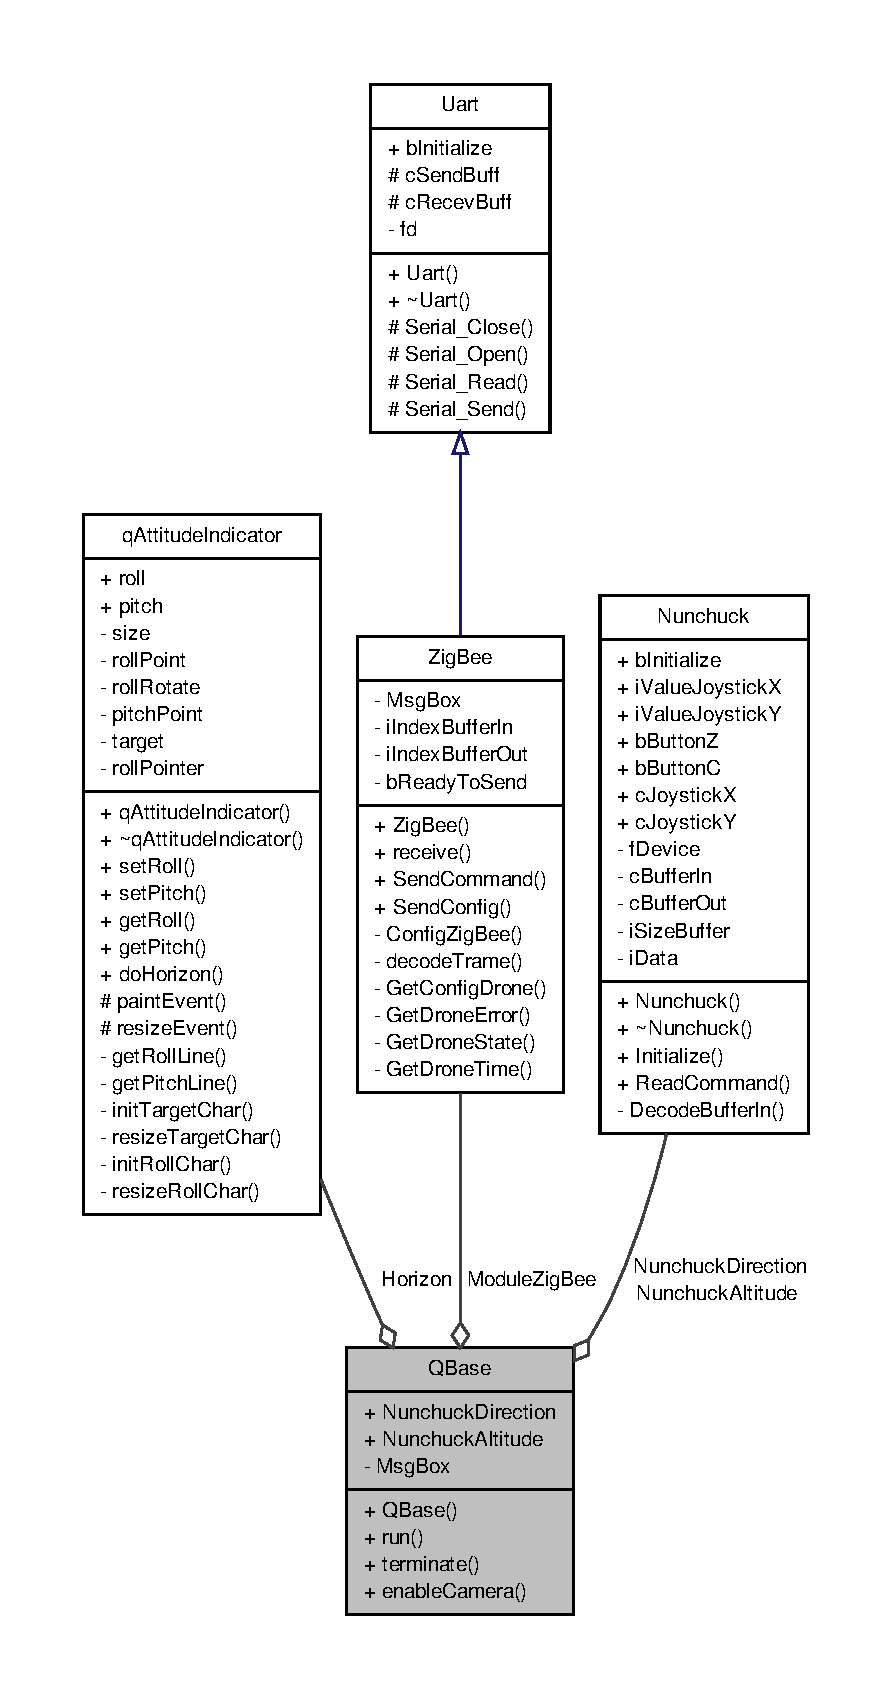
\includegraphics[height=550pt]{classQBase__coll__graph}
\end{center}
\end{figure}
\subsection*{Public Slots}
\begin{DoxyCompactItemize}
\item 
void \hyperlink{classQBase_aeee57e313567e3c333d67e827228862a}{enable\-Camera} (bool b\-Enable)
\end{DoxyCompactItemize}
\subsection*{Public Member Functions}
\begin{DoxyCompactItemize}
\item 
\hyperlink{classQBase_a1951eae68b1eccba818635173cb4eaad}{Q\-Base} (Q\-Object $\ast$parent=0)
\item 
void \hyperlink{classQBase_ac0bbfb1690ac79a226ba59bd7834cdfc}{run} ()
\item 
void \hyperlink{classQBase_a53260534a66388d4b958bd017ebd0f32}{terminate} ()
\end{DoxyCompactItemize}
\subsection*{Public Attributes}
\begin{DoxyCompactItemize}
\item 
\hyperlink{classqAttitudeIndicator}{q\-Attitude\-Indicator} $\ast$ \hyperlink{classQBase_ae4a8b78621695d9a61c311d422824a8d}{Horizon}
\item 
\hyperlink{classNunchuck}{Nunchuck} $\ast$ \hyperlink{classQBase_aa39545ef1795a91bf18db836cde0640d}{Nunchuck\-Direction}
\item 
\hyperlink{classNunchuck}{Nunchuck} $\ast$ \hyperlink{classQBase_a615289f4d92be86986421ec16182ed90}{Nunchuck\-Altitude}
\item 
\hyperlink{classZigBee}{Zig\-Bee} $\ast$ \hyperlink{classQBase_a466b6191fec7cd0029dfc547a5437752}{Module\-Zig\-Bee}
\end{DoxyCompactItemize}
\subsection*{Private Attributes}
\begin{DoxyCompactItemize}
\item 
Q\-Message\-Box \hyperlink{classQBase_aa75e9465559d8633736c52dae36ce1d0}{Msg\-Box}
\end{DoxyCompactItemize}


\subsection{Detailed Description}


Definition at line 10 of file qbase.\-h.



\subsection{Constructor \& Destructor Documentation}
\hypertarget{classQBase_a1951eae68b1eccba818635173cb4eaad}{\index{Q\-Base@{Q\-Base}!Q\-Base@{Q\-Base}}
\index{Q\-Base@{Q\-Base}!QBase@{Q\-Base}}
\subsubsection[{Q\-Base}]{\setlength{\rightskip}{0pt plus 5cm}Q\-Base\-::\-Q\-Base (
\begin{DoxyParamCaption}
\item[{Q\-Object $\ast$}]{parent = {\ttfamily 0}}
\end{DoxyParamCaption}
)\hspace{0.3cm}{\ttfamily [explicit]}}}\label{classQBase_a1951eae68b1eccba818635173cb4eaad}


Definition at line 7 of file qbase.\-cpp.



References Uart\-::b\-Initialize, Nunchuck\-::b\-Initialize, Horizon, Nunchuck\-::\-Initialize(), Module\-Zig\-Bee, Msg\-Box, Nunchuck\-Altitude, Nunchuck\-Direction, P\-A\-R\-A\-M\-\_\-\-A\-L\-T\-I\-T\-U\-D\-E, and P\-A\-R\-A\-M\-\_\-\-D\-I\-R\-E\-C\-T\-I\-O\-N.


\begin{DoxyCode}
                            :
    QThread(parent)
\{
    \hyperlink{classQBase_ae4a8b78621695d9a61c311d422824a8d}{Horizon} = \textcolor{keyword}{new} \hyperlink{classqAttitudeIndicator}{qAttitudeIndicator}();
    \hyperlink{classQBase_aa39545ef1795a91bf18db836cde0640d}{NunchuckDirection} = \textcolor{keyword}{new} \hyperlink{classNunchuck}{Nunchuck}(\hyperlink{nunchuck_8h_abeac51046230d277dc5701b7e45dc88e}{PARAM\_DIRECTION}
      );
    \hyperlink{classQBase_a615289f4d92be86986421ec16182ed90}{NunchuckAltitude} = \textcolor{keyword}{new} \hyperlink{classNunchuck}{Nunchuck}(\hyperlink{nunchuck_8h_af420e9167d30b82b0f623019d165944a}{PARAM\_ALTITUDE}
      );
    \hyperlink{classQBase_a466b6191fec7cd0029dfc547a5437752}{ModuleZigBee} = \textcolor{keyword}{new} \hyperlink{classZigBee}{ZigBee}();


    \textcolor{keywordflow}{if}(!\hyperlink{classQBase_a615289f4d92be86986421ec16182ed90}{NunchuckAltitude}->\hyperlink{classNunchuck_a3ecbcb3a01a247605b4f0a37b579581d}{bInitialize}) \{
        \hyperlink{classQBase_aa75e9465559d8633736c52dae36ce1d0}{MsgBox}.setText(\textcolor{stringliteral}{"Echec de connexion : Commande Altitude\(\backslash\)t\(\backslash\)n       
              (Veuillez la reconnecter)"});
        \hyperlink{classQBase_aa75e9465559d8633736c52dae36ce1d0}{MsgBox}.exec();
        \hyperlink{classQBase_a615289f4d92be86986421ec16182ed90}{NunchuckAltitude}->\hyperlink{classNunchuck_a3ecbcb3a01a247605b4f0a37b579581d}{bInitialize} = 
      \hyperlink{classQBase_a615289f4d92be86986421ec16182ed90}{NunchuckAltitude}->\hyperlink{classNunchuck_aabc3105bbe185edb4521506e5da3dc48}{Initialize}(\hyperlink{nunchuck_8h_af420e9167d30b82b0f623019d165944a}{PARAM\_ALTITUDE}
      );

        \textcolor{keywordflow}{if}(!\hyperlink{classQBase_a615289f4d92be86986421ec16182ed90}{NunchuckAltitude}->\hyperlink{classNunchuck_a3ecbcb3a01a247605b4f0a37b579581d}{bInitialize}) \{
            \hyperlink{classQBase_aa75e9465559d8633736c52dae36ce1d0}{MsgBox}.setText(\textcolor{stringliteral}{"Echec de connexion : Commande Altitude\(\backslash\)t\(\backslash\)n   
                  (Abandon)"});
            \hyperlink{classQBase_aa75e9465559d8633736c52dae36ce1d0}{MsgBox}.exec();
        \}
    \}

    \textcolor{keywordflow}{if}(!\hyperlink{classQBase_aa39545ef1795a91bf18db836cde0640d}{NunchuckDirection}->\hyperlink{classNunchuck_a3ecbcb3a01a247605b4f0a37b579581d}{bInitialize}) \{
        \hyperlink{classQBase_aa75e9465559d8633736c52dae36ce1d0}{MsgBox}.setText(\textcolor{stringliteral}{"Echec de connexion : Commande Direction\(\backslash\)t\(\backslash\)n      
               (Veuillez la reconnecter)"});
        \hyperlink{classQBase_aa75e9465559d8633736c52dae36ce1d0}{MsgBox}.exec();
        \hyperlink{classQBase_aa39545ef1795a91bf18db836cde0640d}{NunchuckDirection}->\hyperlink{classNunchuck_a3ecbcb3a01a247605b4f0a37b579581d}{bInitialize} = 
      \hyperlink{classQBase_aa39545ef1795a91bf18db836cde0640d}{NunchuckDirection}->\hyperlink{classNunchuck_aabc3105bbe185edb4521506e5da3dc48}{Initialize}(\hyperlink{nunchuck_8h_abeac51046230d277dc5701b7e45dc88e}{PARAM\_DIRECTION}
      );

        \textcolor{keywordflow}{if}(!\hyperlink{classQBase_aa39545ef1795a91bf18db836cde0640d}{NunchuckDirection}->\hyperlink{classNunchuck_a3ecbcb3a01a247605b4f0a37b579581d}{bInitialize}) \{
            \hyperlink{classQBase_aa75e9465559d8633736c52dae36ce1d0}{MsgBox}.setText(\textcolor{stringliteral}{"Echec de connexion : Commande Direction\(\backslash\)t\(\backslash\)n  
                   (Abandon)"});
            \hyperlink{classQBase_aa75e9465559d8633736c52dae36ce1d0}{MsgBox}.exec();
        \}
    \}

    \textcolor{keywordflow}{if}(!\hyperlink{classQBase_a466b6191fec7cd0029dfc547a5437752}{ModuleZigBee}->\hyperlink{classUart_a082b349fdf73dd9f4e1a2f1a09af28c3}{bInitialize}) \{
        \hyperlink{classQBase_aa75e9465559d8633736c52dae36ce1d0}{MsgBox}.setText(\textcolor{stringliteral}{"Echec de connexion : Module de Communication\(\backslash\)t\(\backslash\)n 
                  (Abandon)"});
        \hyperlink{classQBase_aa75e9465559d8633736c52dae36ce1d0}{MsgBox}.exec();
    \}
\}
\end{DoxyCode}


\subsection{Member Function Documentation}
\hypertarget{classQBase_aeee57e313567e3c333d67e827228862a}{\index{Q\-Base@{Q\-Base}!enable\-Camera@{enable\-Camera}}
\index{enable\-Camera@{enable\-Camera}!QBase@{Q\-Base}}
\subsubsection[{enable\-Camera}]{\setlength{\rightskip}{0pt plus 5cm}void Q\-Base\-::enable\-Camera (
\begin{DoxyParamCaption}
\item[{bool}]{b\-Enable}
\end{DoxyParamCaption}
)\hspace{0.3cm}{\ttfamily [slot]}}}\label{classQBase_aeee57e313567e3c333d67e827228862a}


Definition at line 222 of file qbase.\-cpp.


\begin{DoxyCode}
\{

\}
\end{DoxyCode}
\hypertarget{classQBase_ac0bbfb1690ac79a226ba59bd7834cdfc}{\index{Q\-Base@{Q\-Base}!run@{run}}
\index{run@{run}!QBase@{Q\-Base}}
\subsubsection[{run}]{\setlength{\rightskip}{0pt plus 5cm}void Q\-Base\-::run (
\begin{DoxyParamCaption}
{}
\end{DoxyParamCaption}
)}}\label{classQBase_ac0bbfb1690ac79a226ba59bd7834cdfc}


Definition at line 44 of file qbase.\-cpp.



References Nunchuck\-::b\-Button\-C, Nunchuck\-::b\-Button\-Z, Nunchuck\-::b\-Initialize, Nunchuck\-::c\-Joystick\-X, Nunchuck\-::c\-Joystick\-Y, q\-Attitude\-Indicator\-::do\-Horizon(), Horizon, J\-B\-A\-S, J\-B\-A\-S\-\_\-\-M\-A\-X, J\-C\-E\-N\-T\-R\-E, J\-D\-R\-O\-I\-T\-E, J\-D\-R\-O\-I\-T\-E\-\_\-\-M\-A\-X, J\-G\-A\-U\-C\-H\-E, J\-G\-A\-U\-C\-H\-E\-\_\-\-M\-A\-X, J\-H\-A\-U\-T, J\-H\-A\-U\-T\-\_\-\-M\-A\-X, Module\-Zig\-Bee, Nunchuck\-Altitude, Nunchuck\-Direction, q\-Attitude\-Indicator\-::pitch, Nunchuck\-::\-Read\-Command(), Zig\-Bee\-::receive(), q\-Attitude\-Indicator\-::roll, and Zig\-Bee\-::\-Send\-Command().


\begin{DoxyCode}
\{
    \textcolor{comment}{//Doit attendre l'information de démarrage du drone : puis emettre toutes
       les 500ms}
    \textcolor{comment}{//Pourrait émettre toutes les 500ms, 250ms avant que le drone écoute?.
       (voir fonction boquante read)}
    \textcolor{comment}{//FONCTION DE SINCRONISATION !!}
    QTime time;
    QString Qtmp;
    std::ofstream    f(\textcolor{stringliteral}{"/tmp/LogZigBee"}, std::ios\_base::app);

    time.start();

    \textcolor{keywordflow}{while} (1) \{

        \textcolor{comment}{/* Recupère les données des commandes */}
        \textcolor{keywordflow}{if}(\hyperlink{classQBase_aa39545ef1795a91bf18db836cde0640d}{NunchuckDirection}->\hyperlink{classNunchuck_a3ecbcb3a01a247605b4f0a37b579581d}{bInitialize})
            \hyperlink{classQBase_aa39545ef1795a91bf18db836cde0640d}{NunchuckDirection}->\hyperlink{classNunchuck_ade6607a55fda6ae67c90d3d1ee7ce56b}{ReadCommand}();

        \textcolor{keywordflow}{if}(\hyperlink{classQBase_aa39545ef1795a91bf18db836cde0640d}{NunchuckDirection}->\hyperlink{classNunchuck_a0db1f3d2f58fafda23a5af3936c12598}{bButtonZ}) \{

        \}

        \textcolor{keywordflow}{if}(\hyperlink{classQBase_aa39545ef1795a91bf18db836cde0640d}{NunchuckDirection}->\hyperlink{classNunchuck_a1d5cac3b603b3060984e3184d795561d}{bButtonC}) \{

        \}

        \textcolor{comment}{/* Mise à jour des commandes de vol et de l'Horizon(pour test) */}
        \textcolor{keywordflow}{switch} (\hyperlink{classQBase_aa39545ef1795a91bf18db836cde0640d}{NunchuckDirection}->\hyperlink{classNunchuck_ad9467642b97b8b008ddd137d273a22f8}{cJoystickX}) \{
        \textcolor{keywordflow}{case} \hyperlink{nunchuck_8h_ac63506adba6ed764c5061ac249623554}{JCENTRE}:
            \hyperlink{classQBase_ae4a8b78621695d9a61c311d422824a8d}{Horizon}->\hyperlink{classqAttitudeIndicator_a10c98e2fd9195050cb305f4b12bf75bb}{roll} = 0.0;
            \textcolor{comment}{/* Mise à jour des commandes de vol */}
            \hyperlink{classQBase_a466b6191fec7cd0029dfc547a5437752}{ModuleZigBee}->st\_CommandDrone.cTransY = 0;    \textcolor{comment}{//
      Vérifier avec Nabil!!!}
            \textcolor{keywordflow}{break};
        \textcolor{keywordflow}{case} \hyperlink{nunchuck_8h_abb937f82823e628ca09a026777179226}{JDROITE}:
            \hyperlink{classQBase_ae4a8b78621695d9a61c311d422824a8d}{Horizon}->\hyperlink{classqAttitudeIndicator_a10c98e2fd9195050cb305f4b12bf75bb}{roll} = -15.0;
            \textcolor{comment}{/* Mise à jour des commandes de vol */}
            \hyperlink{classQBase_a466b6191fec7cd0029dfc547a5437752}{ModuleZigBee}->st\_CommandDrone.cTransY = 1;    \textcolor{comment}{//
      Vérifier avec Nabil!!!}
            \textcolor{keywordflow}{break};
        \textcolor{keywordflow}{case} \hyperlink{nunchuck_8h_a2948a7fb931671c2935a67be056ec44d}{JGAUCHE}:
            \hyperlink{classQBase_ae4a8b78621695d9a61c311d422824a8d}{Horizon}->\hyperlink{classqAttitudeIndicator_a10c98e2fd9195050cb305f4b12bf75bb}{roll} = 15.0;
            \textcolor{comment}{/* Mise à jour des commandes de vol */}
            \hyperlink{classQBase_a466b6191fec7cd0029dfc547a5437752}{ModuleZigBee}->st\_CommandDrone.cTransY = -1;    \textcolor{comment}{//
      Vérifier avec Nabil!!!}
            \textcolor{keywordflow}{break};
        \textcolor{keywordflow}{case} \hyperlink{nunchuck_8h_a13baf3bab74f21c7050fb8029bf5b871}{JDROITE\_MAX}:
            \hyperlink{classQBase_ae4a8b78621695d9a61c311d422824a8d}{Horizon}->\hyperlink{classqAttitudeIndicator_a10c98e2fd9195050cb305f4b12bf75bb}{roll} = -30.0;
            \textcolor{comment}{/* Mise à jour des commandes de vol */}
            \hyperlink{classQBase_a466b6191fec7cd0029dfc547a5437752}{ModuleZigBee}->st\_CommandDrone.cTransY = 2;    \textcolor{comment}{//
      Vérifier avec Nabil!!!}
            \textcolor{keywordflow}{break};
        \textcolor{keywordflow}{case} \hyperlink{nunchuck_8h_a19f4efb3793bd7fd7da3a60339dc4631}{JGAUCHE\_MAX}:
            \hyperlink{classQBase_ae4a8b78621695d9a61c311d422824a8d}{Horizon}->\hyperlink{classqAttitudeIndicator_a10c98e2fd9195050cb305f4b12bf75bb}{roll} = 30.0;
            \textcolor{comment}{/* Mise à jour des commandes de vol */}
            \hyperlink{classQBase_a466b6191fec7cd0029dfc547a5437752}{ModuleZigBee}->st\_CommandDrone.cTransY = -2;    \textcolor{comment}{//
      Vérifier avec Nabil!!!}
            \textcolor{keywordflow}{break};
        \textcolor{keywordflow}{default}:
            \hyperlink{classQBase_ae4a8b78621695d9a61c311d422824a8d}{Horizon}->\hyperlink{classqAttitudeIndicator_a10c98e2fd9195050cb305f4b12bf75bb}{roll} = 90.0;
            \textcolor{comment}{/* Mise à jour des commandes de vol */}
            \hyperlink{classQBase_a466b6191fec7cd0029dfc547a5437752}{ModuleZigBee}->st\_CommandDrone.cTransY = 0;    \textcolor{comment}{//
      Vérifier avec Nabil!!!}
            \textcolor{keywordflow}{break};
        \}

        \textcolor{keywordflow}{switch} (\hyperlink{classQBase_aa39545ef1795a91bf18db836cde0640d}{NunchuckDirection}->\hyperlink{classNunchuck_aaf0f299016f5acf686f716518a7ce567}{cJoystickY}) \{
        \textcolor{keywordflow}{case} \hyperlink{nunchuck_8h_ac63506adba6ed764c5061ac249623554}{JCENTRE}:
            \hyperlink{classQBase_ae4a8b78621695d9a61c311d422824a8d}{Horizon}->\hyperlink{classqAttitudeIndicator_ae0df6492b15cc2d3f51c3de0e6dd08bd}{pitch} = 0.0;
            \textcolor{comment}{/* Mise à jour des commandes de vol */}
            \hyperlink{classQBase_a466b6191fec7cd0029dfc547a5437752}{ModuleZigBee}->st\_CommandDrone.cTransX = 0;    \textcolor{comment}{//
      Vérifier avec Nabil!!!}
            \textcolor{keywordflow}{break};
        \textcolor{keywordflow}{case} \hyperlink{nunchuck_8h_a624208e4279eb8508e4d7a4cd1983293}{JHAUT}:
            \hyperlink{classQBase_ae4a8b78621695d9a61c311d422824a8d}{Horizon}->\hyperlink{classqAttitudeIndicator_ae0df6492b15cc2d3f51c3de0e6dd08bd}{pitch} = 10.0;
            \textcolor{comment}{/* Mise à jour des commandes de vol */}
            \hyperlink{classQBase_a466b6191fec7cd0029dfc547a5437752}{ModuleZigBee}->st\_CommandDrone.cTransX = -1;    \textcolor{comment}{//
      Vérifier avec Nabil!!!}
            \textcolor{keywordflow}{break};
        \textcolor{keywordflow}{case} \hyperlink{nunchuck_8h_ad9a8fe51b03c91dc0256cc7502d450a3}{JBAS}:
            \hyperlink{classQBase_ae4a8b78621695d9a61c311d422824a8d}{Horizon}->\hyperlink{classqAttitudeIndicator_ae0df6492b15cc2d3f51c3de0e6dd08bd}{pitch} = -10.0;
            \textcolor{comment}{/* Mise à jour des commandes de vol */}
            \hyperlink{classQBase_a466b6191fec7cd0029dfc547a5437752}{ModuleZigBee}->st\_CommandDrone.cTransX = 1;    \textcolor{comment}{//
      Vérifier avec Nabil!!!}
            \textcolor{keywordflow}{break};
        \textcolor{keywordflow}{case} \hyperlink{nunchuck_8h_a69c726c7ddc8415a81ea58834356ed2b}{JHAUT\_MAX}:
            \hyperlink{classQBase_ae4a8b78621695d9a61c311d422824a8d}{Horizon}->\hyperlink{classqAttitudeIndicator_ae0df6492b15cc2d3f51c3de0e6dd08bd}{pitch} = 20.0;
            \textcolor{comment}{/* Mise à jour des commandes de vol */}
            \hyperlink{classQBase_a466b6191fec7cd0029dfc547a5437752}{ModuleZigBee}->st\_CommandDrone.cTransX = -2;    \textcolor{comment}{//
      Vérifier avec Nabil!!!}
            \textcolor{keywordflow}{break};
        \textcolor{keywordflow}{case} \hyperlink{nunchuck_8h_a8bd0c46505c3f0a7d5bc412d8a56d41a}{JBAS\_MAX}:
            \hyperlink{classQBase_ae4a8b78621695d9a61c311d422824a8d}{Horizon}->\hyperlink{classqAttitudeIndicator_ae0df6492b15cc2d3f51c3de0e6dd08bd}{pitch} = -20.0;
            \textcolor{comment}{/* Mise à jour des commandes de vol */}
            \hyperlink{classQBase_a466b6191fec7cd0029dfc547a5437752}{ModuleZigBee}->st\_CommandDrone.cTransX = 2;    \textcolor{comment}{//
      Vérifier avec Nabil!!!}
            \textcolor{keywordflow}{break};
        \textcolor{keywordflow}{default}:
            \hyperlink{classQBase_ae4a8b78621695d9a61c311d422824a8d}{Horizon}->\hyperlink{classqAttitudeIndicator_ae0df6492b15cc2d3f51c3de0e6dd08bd}{pitch} = 90.0;
            \textcolor{comment}{/* Mise à jour des commandes de vol */}
            \hyperlink{classQBase_a466b6191fec7cd0029dfc547a5437752}{ModuleZigBee}->st\_CommandDrone.cTransX = 0;    \textcolor{comment}{//
      Vérifier avec Nabil!!!}
            \textcolor{keywordflow}{break};
        \}
        \hyperlink{classQBase_ae4a8b78621695d9a61c311d422824a8d}{Horizon}->\hyperlink{classqAttitudeIndicator_a7d4e7b19bc493de63a91b0e0480c24e2}{doHorizon}();

        \textcolor{keywordflow}{switch} (\hyperlink{classQBase_a615289f4d92be86986421ec16182ed90}{NunchuckAltitude}->\hyperlink{classNunchuck_ad9467642b97b8b008ddd137d273a22f8}{cJoystickX}) \{
        \textcolor{keywordflow}{case} \hyperlink{nunchuck_8h_ac63506adba6ed764c5061ac249623554}{JCENTRE}:
            \textcolor{comment}{/* Mise à jour des commandes de vol */}
            \hyperlink{classQBase_a466b6191fec7cd0029dfc547a5437752}{ModuleZigBee}->st\_CommandDrone.cRotZ = 0;    \textcolor{comment}{//Vérifier
       avec Nabil!!!}
            \textcolor{keywordflow}{break};
        \textcolor{keywordflow}{case} \hyperlink{nunchuck_8h_abb937f82823e628ca09a026777179226}{JDROITE}:
            \textcolor{comment}{/* Mise à jour des commandes de vol */}
            \hyperlink{classQBase_a466b6191fec7cd0029dfc547a5437752}{ModuleZigBee}->st\_CommandDrone.cRotZ = 1;    \textcolor{comment}{//Vérifier
       avec Nabil!!!}
            \textcolor{keywordflow}{break};
        \textcolor{keywordflow}{case} \hyperlink{nunchuck_8h_a2948a7fb931671c2935a67be056ec44d}{JGAUCHE}:
            \textcolor{comment}{/* Mise à jour des commandes de vol */}
            \hyperlink{classQBase_a466b6191fec7cd0029dfc547a5437752}{ModuleZigBee}->st\_CommandDrone.cRotZ = -1;    \textcolor{comment}{//Vérifier
       avec Nabil!!!}
            \textcolor{keywordflow}{break};
        \textcolor{keywordflow}{case} \hyperlink{nunchuck_8h_a13baf3bab74f21c7050fb8029bf5b871}{JDROITE\_MAX}:
            \textcolor{comment}{/* Mise à jour des commandes de vol */}
            \hyperlink{classQBase_a466b6191fec7cd0029dfc547a5437752}{ModuleZigBee}->st\_CommandDrone.cRotZ = 2;    \textcolor{comment}{//Vérifier
       avec Nabil!!!}
            \textcolor{keywordflow}{break};
        \textcolor{keywordflow}{case} \hyperlink{nunchuck_8h_a19f4efb3793bd7fd7da3a60339dc4631}{JGAUCHE\_MAX}:
            \textcolor{comment}{/* Mise à jour des commandes de vol */}
            \hyperlink{classQBase_a466b6191fec7cd0029dfc547a5437752}{ModuleZigBee}->st\_CommandDrone.cRotZ = -2;    \textcolor{comment}{//Vérifier
       avec Nabil!!!}
            \textcolor{keywordflow}{break};
        \textcolor{keywordflow}{default}:
            \textcolor{comment}{/* Mise à jour des commandes de vol */}
            \hyperlink{classQBase_a466b6191fec7cd0029dfc547a5437752}{ModuleZigBee}->st\_CommandDrone.cRotZ = 0;    \textcolor{comment}{//Vérifier
       avec Nabil!!!}
            \textcolor{keywordflow}{break};
        \}

        \textcolor{keywordflow}{switch} (\hyperlink{classQBase_a615289f4d92be86986421ec16182ed90}{NunchuckAltitude}->\hyperlink{classNunchuck_aaf0f299016f5acf686f716518a7ce567}{cJoystickY}) \{
        \textcolor{keywordflow}{case} \hyperlink{nunchuck_8h_ac63506adba6ed764c5061ac249623554}{JCENTRE}:
            \textcolor{comment}{/* Mise à jour des commandes de vol */}
            \hyperlink{classQBase_a466b6191fec7cd0029dfc547a5437752}{ModuleZigBee}->st\_CommandDrone.cTransZ = 0;    \textcolor{comment}{//
      Vérifier avec Nabil!!!}
            \textcolor{keywordflow}{break};
        \textcolor{keywordflow}{case} \hyperlink{nunchuck_8h_a624208e4279eb8508e4d7a4cd1983293}{JHAUT}:
            \textcolor{comment}{/* Mise à jour des commandes de vol */}
            \hyperlink{classQBase_a466b6191fec7cd0029dfc547a5437752}{ModuleZigBee}->st\_CommandDrone.cTransZ = 1;    \textcolor{comment}{//
      Vérifier avec Nabil!!!}
            \textcolor{keywordflow}{break};
        \textcolor{keywordflow}{case} \hyperlink{nunchuck_8h_ad9a8fe51b03c91dc0256cc7502d450a3}{JBAS}:
            \textcolor{comment}{/* Mise à jour des commandes de vol */}
            \hyperlink{classQBase_a466b6191fec7cd0029dfc547a5437752}{ModuleZigBee}->st\_CommandDrone.cTransZ = -1;    \textcolor{comment}{//
      Vérifier avec Nabil!!!}
            \textcolor{keywordflow}{break};
        \textcolor{keywordflow}{case} \hyperlink{nunchuck_8h_a69c726c7ddc8415a81ea58834356ed2b}{JHAUT\_MAX}:
            \textcolor{comment}{/* Mise à jour des commandes de vol */}
            \hyperlink{classQBase_a466b6191fec7cd0029dfc547a5437752}{ModuleZigBee}->st\_CommandDrone.cTransZ = 2;    \textcolor{comment}{//
      Vérifier avec Nabil!!!}
            \textcolor{keywordflow}{break};
        \textcolor{keywordflow}{case} \hyperlink{nunchuck_8h_a8bd0c46505c3f0a7d5bc412d8a56d41a}{JBAS\_MAX}:
            \textcolor{comment}{/* Mise à jour des commandes de vol */}
            \hyperlink{classQBase_a466b6191fec7cd0029dfc547a5437752}{ModuleZigBee}->st\_CommandDrone.cTransZ = -2;    \textcolor{comment}{//
      Vérifier avec Nabil!!!}
            \textcolor{keywordflow}{break};
        \textcolor{keywordflow}{default}:
            \textcolor{comment}{/* Mise à jour des commandes de vol */}
            \hyperlink{classQBase_a466b6191fec7cd0029dfc547a5437752}{ModuleZigBee}->st\_CommandDrone.cTransZ = 0;    \textcolor{comment}{//
      Vérifier avec Nabil!!!}
            \textcolor{keywordflow}{break};
        \}

        \textcolor{comment}{//if(SET\_CONFIG\_TO\_DRONE) \{}
            \textcolor{comment}{//OPEN\_WINDOW\_CONFIG AND SEND CONFIG}
            \textcolor{comment}{//ModuleZigBee->SendConfig();}
        \textcolor{comment}{//\}}
        \textcolor{comment}{//else \{}
            Qtmp.sprintf(\textcolor{stringliteral}{"Time before send : %d\(\backslash\)n"},time.elapsed());
            f.write(Qtmp.toStdString().c\_str(), Qtmp.length());
            \hyperlink{classQBase_a466b6191fec7cd0029dfc547a5437752}{ModuleZigBee}->\hyperlink{classZigBee_a6b69e04be626400b5b245fa1b56f0810}{SendCommand}();

        \textcolor{comment}{//\}}
        Qtmp.sprintf(\textcolor{stringliteral}{"Time before receive : %d\(\backslash\)n"},time.elapsed());
        f.write(Qtmp.toStdString().c\_str(), Qtmp.length());
        \textcolor{comment}{//printf("%s\(\backslash\)n",Qtmp.toStdString().c\_str());}
        \hyperlink{classQBase_a466b6191fec7cd0029dfc547a5437752}{ModuleZigBee}->\hyperlink{classZigBee_a0852f85771d48df17a6256edcd91bece}{receive}();
        Qtmp.sprintf(\textcolor{stringliteral}{"Time after receive : %d\(\backslash\)n"},time.elapsed());
        f.write(Qtmp.toStdString().c\_str(), Qtmp.length());

        usleep(50000);\textcolor{comment}{//Pour ralentir le programme...}
        time.restart();

    \}
\}
\end{DoxyCode}
\hypertarget{classQBase_a53260534a66388d4b958bd017ebd0f32}{\index{Q\-Base@{Q\-Base}!terminate@{terminate}}
\index{terminate@{terminate}!QBase@{Q\-Base}}
\subsubsection[{terminate}]{\setlength{\rightskip}{0pt plus 5cm}void Q\-Base\-::terminate (
\begin{DoxyParamCaption}
{}
\end{DoxyParamCaption}
)}}\label{classQBase_a53260534a66388d4b958bd017ebd0f32}


Definition at line 214 of file qbase.\-cpp.



References Horizon, Module\-Zig\-Bee, Nunchuck\-Altitude, and Nunchuck\-Direction.


\begin{DoxyCode}
\{
    \textcolor{keyword}{delete} \hyperlink{classQBase_a466b6191fec7cd0029dfc547a5437752}{ModuleZigBee};
    \textcolor{keyword}{delete} \hyperlink{classQBase_aa39545ef1795a91bf18db836cde0640d}{NunchuckDirection};
    \textcolor{keyword}{delete} \hyperlink{classQBase_a615289f4d92be86986421ec16182ed90}{NunchuckAltitude};
    \textcolor{keyword}{delete} \hyperlink{classQBase_ae4a8b78621695d9a61c311d422824a8d}{Horizon};
\}
\end{DoxyCode}


\subsection{Member Data Documentation}
\hypertarget{classQBase_ae4a8b78621695d9a61c311d422824a8d}{\index{Q\-Base@{Q\-Base}!Horizon@{Horizon}}
\index{Horizon@{Horizon}!QBase@{Q\-Base}}
\subsubsection[{Horizon}]{\setlength{\rightskip}{0pt plus 5cm}{\bf q\-Attitude\-Indicator}$\ast$ Q\-Base\-::\-Horizon}}\label{classQBase_ae4a8b78621695d9a61c311d422824a8d}


Definition at line 19 of file qbase.\-h.



Referenced by Main\-Window\-::\-Change\-Onglet(), Q\-Base(), run(), and terminate().

\hypertarget{classQBase_a466b6191fec7cd0029dfc547a5437752}{\index{Q\-Base@{Q\-Base}!Module\-Zig\-Bee@{Module\-Zig\-Bee}}
\index{Module\-Zig\-Bee@{Module\-Zig\-Bee}!QBase@{Q\-Base}}
\subsubsection[{Module\-Zig\-Bee}]{\setlength{\rightskip}{0pt plus 5cm}{\bf Zig\-Bee}$\ast$ Q\-Base\-::\-Module\-Zig\-Bee}}\label{classQBase_a466b6191fec7cd0029dfc547a5437752}


Definition at line 22 of file qbase.\-h.



Referenced by Q\-Base(), run(), and terminate().

\hypertarget{classQBase_aa75e9465559d8633736c52dae36ce1d0}{\index{Q\-Base@{Q\-Base}!Msg\-Box@{Msg\-Box}}
\index{Msg\-Box@{Msg\-Box}!QBase@{Q\-Base}}
\subsubsection[{Msg\-Box}]{\setlength{\rightskip}{0pt plus 5cm}Q\-Message\-Box Q\-Base\-::\-Msg\-Box\hspace{0.3cm}{\ttfamily [private]}}}\label{classQBase_aa75e9465559d8633736c52dae36ce1d0}


Definition at line 24 of file qbase.\-h.



Referenced by Q\-Base().

\hypertarget{classQBase_a615289f4d92be86986421ec16182ed90}{\index{Q\-Base@{Q\-Base}!Nunchuck\-Altitude@{Nunchuck\-Altitude}}
\index{Nunchuck\-Altitude@{Nunchuck\-Altitude}!QBase@{Q\-Base}}
\subsubsection[{Nunchuck\-Altitude}]{\setlength{\rightskip}{0pt plus 5cm}{\bf Nunchuck}$\ast$ Q\-Base\-::\-Nunchuck\-Altitude}}\label{classQBase_a615289f4d92be86986421ec16182ed90}


Definition at line 21 of file qbase.\-h.



Referenced by Q\-Base(), run(), and terminate().

\hypertarget{classQBase_aa39545ef1795a91bf18db836cde0640d}{\index{Q\-Base@{Q\-Base}!Nunchuck\-Direction@{Nunchuck\-Direction}}
\index{Nunchuck\-Direction@{Nunchuck\-Direction}!QBase@{Q\-Base}}
\subsubsection[{Nunchuck\-Direction}]{\setlength{\rightskip}{0pt plus 5cm}{\bf Nunchuck}$\ast$ Q\-Base\-::\-Nunchuck\-Direction}}\label{classQBase_aa39545ef1795a91bf18db836cde0640d}


Definition at line 20 of file qbase.\-h.



Referenced by Q\-Base(), run(), and terminate().



The documentation for this class was generated from the following files\-:\begin{DoxyCompactItemize}
\item 
\hyperlink{qbase_8h}{qbase.\-h}\item 
\hyperlink{qbase_8cpp}{qbase.\-cpp}\end{DoxyCompactItemize}

\hypertarget{classQTh__Base}{\section{Q\-Th\-\_\-\-Base Class Reference}
\label{classQTh__Base}\index{Q\-Th\-\_\-\-Base@{Q\-Th\-\_\-\-Base}}
}


{\ttfamily \#include \char`\"{}qth\-\_\-base.\-h\char`\"{}}



Collaboration diagram for Q\-Th\-\_\-\-Base\-:\nopagebreak
\begin{figure}[H]
\begin{center}
\leavevmode
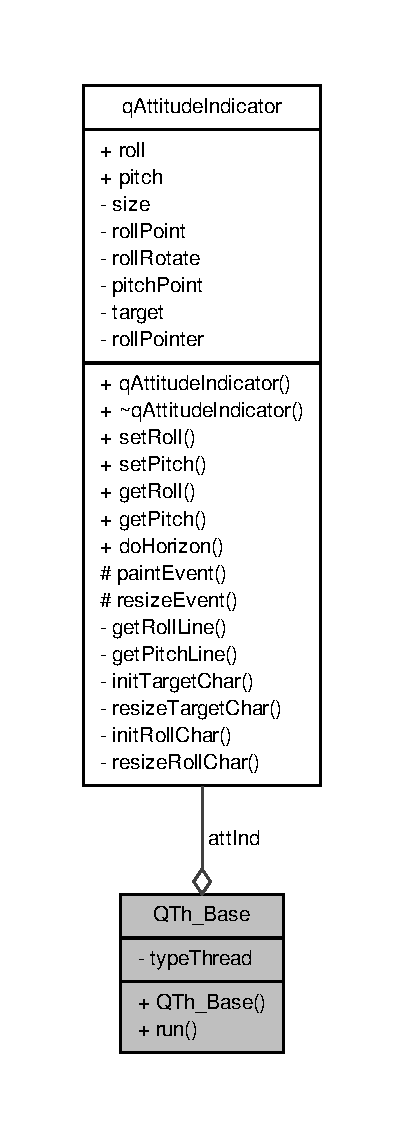
\includegraphics[width=194pt]{classQTh__Base__coll__graph}
\end{center}
\end{figure}
\subsection*{Public Member Functions}
\begin{DoxyCompactItemize}
\item 
\hyperlink{classQTh__Base_a74f0d7d927529f648cb8f5d29059c786}{Q\-Th\-\_\-\-Base} (int type, Q\-Object $\ast$parent=0)
\item 
void \hyperlink{classQTh__Base_a391a2d2c1b79448577333036eb7bc591}{run} ()
\end{DoxyCompactItemize}
\subsection*{Public Attributes}
\begin{DoxyCompactItemize}
\item 
\hyperlink{classqAttitudeIndicator}{q\-Attitude\-Indicator} $\ast$ \hyperlink{classQTh__Base_a51fa634be0cdd712417ee2f97919acc7}{att\-Ind}
\end{DoxyCompactItemize}
\subsection*{Private Attributes}
\begin{DoxyCompactItemize}
\item 
int \hyperlink{classQTh__Base_acc21cc2cc7304e83231c9f305874499f}{type\-Thread}
\end{DoxyCompactItemize}


\subsection{Detailed Description}


Definition at line 10 of file qth\-\_\-base.\-h.



\subsection{Constructor \& Destructor Documentation}
\hypertarget{classQTh__Base_a74f0d7d927529f648cb8f5d29059c786}{\index{Q\-Th\-\_\-\-Base@{Q\-Th\-\_\-\-Base}!Q\-Th\-\_\-\-Base@{Q\-Th\-\_\-\-Base}}
\index{Q\-Th\-\_\-\-Base@{Q\-Th\-\_\-\-Base}!QTh_Base@{Q\-Th\-\_\-\-Base}}
\subsubsection[{Q\-Th\-\_\-\-Base}]{\setlength{\rightskip}{0pt plus 5cm}Q\-Th\-\_\-\-Base\-::\-Q\-Th\-\_\-\-Base (
\begin{DoxyParamCaption}
\item[{int}]{type, }
\item[{Q\-Object $\ast$}]{parent = {\ttfamily 0}}
\end{DoxyParamCaption}
)\hspace{0.3cm}{\ttfamily [explicit]}}}\label{classQTh__Base_a74f0d7d927529f648cb8f5d29059c786}


Definition at line 10 of file qth\-\_\-base.\-cpp.



References att\-Ind, Q\-T\-H\-R\-E\-A\-D\-\_\-\-H\-O\-R\-I\-Z\-O\-N, and type\-Thread.


\begin{DoxyCode}
                                            :
    QThread(parent)
\{
    \hyperlink{classQTh__Base_acc21cc2cc7304e83231c9f305874499f}{typeThread} = type;

    \textcolor{keywordflow}{switch}(\hyperlink{classQTh__Base_acc21cc2cc7304e83231c9f305874499f}{typeThread}) \{

    \textcolor{keywordflow}{case} \hyperlink{qth__base_8h_a2f3670a7586687feccfde021b896c2b8}{QTHREAD\_HORIZON}:
        \hyperlink{classQTh__Base_a51fa634be0cdd712417ee2f97919acc7}{attInd} = \textcolor{keyword}{new} \hyperlink{classqAttitudeIndicator}{qAttitudeIndicator}();
        \textcolor{keywordflow}{break};

    \textcolor{keywordflow}{default}:
        \textcolor{keywordflow}{break};
    \}
\}
\end{DoxyCode}


\subsection{Member Function Documentation}
\hypertarget{classQTh__Base_a391a2d2c1b79448577333036eb7bc591}{\index{Q\-Th\-\_\-\-Base@{Q\-Th\-\_\-\-Base}!run@{run}}
\index{run@{run}!QTh_Base@{Q\-Th\-\_\-\-Base}}
\subsubsection[{run}]{\setlength{\rightskip}{0pt plus 5cm}void Q\-Th\-\_\-\-Base\-::run (
\begin{DoxyParamCaption}
{}
\end{DoxyParamCaption}
)}}\label{classQTh__Base_a391a2d2c1b79448577333036eb7bc591}


Definition at line 26 of file qth\-\_\-base.\-cpp.



References att\-Ind, q\-Attitude\-Indicator\-::do\-Horizon(), Q\-T\-H\-R\-E\-A\-D\-\_\-\-H\-O\-R\-I\-Z\-O\-N, and type\-Thread.


\begin{DoxyCode}
\{
\textcolor{comment}{//    switch(typeThread) \{}
\textcolor{comment}{//    case QTHREAD\_HORIZON:}
\textcolor{comment}{//        break;}
\textcolor{comment}{//    default:}
\textcolor{comment}{//        break;}
\textcolor{comment}{//    \}}

    \textcolor{keywordflow}{while} (1) \{
        \textcolor{keywordflow}{switch}(\hyperlink{classQTh__Base_acc21cc2cc7304e83231c9f305874499f}{typeThread}) \{

        \textcolor{keywordflow}{case} \hyperlink{qth__base_8h_a2f3670a7586687feccfde021b896c2b8}{QTHREAD\_HORIZON}:
            \hyperlink{classQTh__Base_a51fa634be0cdd712417ee2f97919acc7}{attInd}->\hyperlink{classqAttitudeIndicator_a7d4e7b19bc493de63a91b0e0480c24e2}{doHorizon}();
            \textcolor{keywordflow}{break};

        \textcolor{keywordflow}{default}:
            \textcolor{keywordflow}{break};
        \}
        msleep(50);
    \}
\}
\end{DoxyCode}


\subsection{Member Data Documentation}
\hypertarget{classQTh__Base_a51fa634be0cdd712417ee2f97919acc7}{\index{Q\-Th\-\_\-\-Base@{Q\-Th\-\_\-\-Base}!att\-Ind@{att\-Ind}}
\index{att\-Ind@{att\-Ind}!QTh_Base@{Q\-Th\-\_\-\-Base}}
\subsubsection[{att\-Ind}]{\setlength{\rightskip}{0pt plus 5cm}{\bf q\-Attitude\-Indicator}$\ast$ Q\-Th\-\_\-\-Base\-::att\-Ind}}\label{classQTh__Base_a51fa634be0cdd712417ee2f97919acc7}


Definition at line 18 of file qth\-\_\-base.\-h.



Referenced by Q\-Th\-\_\-\-Base(), and run().

\hypertarget{classQTh__Base_acc21cc2cc7304e83231c9f305874499f}{\index{Q\-Th\-\_\-\-Base@{Q\-Th\-\_\-\-Base}!type\-Thread@{type\-Thread}}
\index{type\-Thread@{type\-Thread}!QTh_Base@{Q\-Th\-\_\-\-Base}}
\subsubsection[{type\-Thread}]{\setlength{\rightskip}{0pt plus 5cm}int Q\-Th\-\_\-\-Base\-::type\-Thread\hspace{0.3cm}{\ttfamily [private]}}}\label{classQTh__Base_acc21cc2cc7304e83231c9f305874499f}


Definition at line 21 of file qth\-\_\-base.\-h.



Referenced by Q\-Th\-\_\-\-Base(), and run().



The documentation for this class was generated from the following files\-:\begin{DoxyCompactItemize}
\item 
\hyperlink{qth__base_8h}{qth\-\_\-base.\-h}\item 
\hyperlink{qth__base_8cpp}{qth\-\_\-base.\-cpp}\end{DoxyCompactItemize}

\hypertarget{classSlippyMap}{\section{Slippy\-Map Class Reference}
\label{classSlippyMap}\index{Slippy\-Map@{Slippy\-Map}}
}


{\ttfamily \#include \char`\"{}slippymap.\-h\char`\"{}}



Collaboration diagram for Slippy\-Map\-:\nopagebreak
\begin{figure}[H]
\begin{center}
\leavevmode
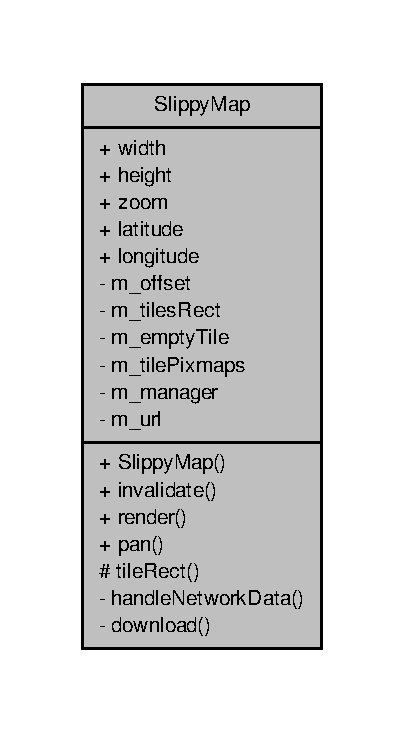
\includegraphics[width=194pt]{classSlippyMap__coll__graph}
\end{center}
\end{figure}
\subsection*{Signals}
\begin{DoxyCompactItemize}
\item 
void \hyperlink{classSlippyMap_a6ff062c778eec629347d834976760c98}{updated} (const Q\-Rect \&rect)
\end{DoxyCompactItemize}
\subsection*{Public Member Functions}
\begin{DoxyCompactItemize}
\item 
\hyperlink{classSlippyMap_aefaa28b154b2e9602b391668ed167080}{Slippy\-Map} (Q\-Object $\ast$parent=0)
\item 
void \hyperlink{classSlippyMap_aa8a2647176ff7db85ab52ce9e7acb549}{invalidate} ()
\item 
void \hyperlink{classSlippyMap_ada1e00e2870d0fdeb70c037b3222a0ad}{render} (Q\-Painter $\ast$p, const Q\-Rect \&rect)
\item 
void \hyperlink{classSlippyMap_ae954bbb164e84e5cecf3fbb518eb266c}{pan} (const Q\-Point \&delta)
\end{DoxyCompactItemize}
\subsection*{Public Attributes}
\begin{DoxyCompactItemize}
\item 
int \hyperlink{classSlippyMap_ada3532095a8c4083e9da3db17de29fc1}{width}
\item 
int \hyperlink{classSlippyMap_aacec4be5e2b83eb2744a3b3b03c4af7a}{height}
\item 
int \hyperlink{classSlippyMap_a13dcc9915570a1a333c1e9275ffe64b3}{zoom}
\item 
qreal \hyperlink{classSlippyMap_a223220fdcbf2197845f009d48225c0c8}{latitude}
\item 
qreal \hyperlink{classSlippyMap_af93efe003c192b7bc6a1ece6c7342de6}{longitude}
\end{DoxyCompactItemize}
\subsection*{Protected Member Functions}
\begin{DoxyCompactItemize}
\item 
Q\-Rect \hyperlink{classSlippyMap_ada0e611fc8d684f9255236237105508d}{tile\-Rect} (const Q\-Point \&tp)
\end{DoxyCompactItemize}
\subsection*{Private Slots}
\begin{DoxyCompactItemize}
\item 
void \hyperlink{classSlippyMap_af069a885b3750deed3ebf1f992426753}{handle\-Network\-Data} (Q\-Network\-Reply $\ast$reply)
\item 
void \hyperlink{classSlippyMap_a25dc08d50224b8aa392adbaa1667bbc1}{download} ()
\end{DoxyCompactItemize}
\subsection*{Private Attributes}
\begin{DoxyCompactItemize}
\item 
Q\-Point \hyperlink{classSlippyMap_a705bb1600f5003868b890f1e25a198a6}{m\-\_\-offset}
\item 
Q\-Rect \hyperlink{classSlippyMap_aa8154d798c574c1d6ed89f3347835a76}{m\-\_\-tiles\-Rect}
\item 
Q\-Pixmap \hyperlink{classSlippyMap_a0021bf8f7ecbaa61bd47f8f0a36ea9d0}{m\-\_\-empty\-Tile}
\item 
Q\-Hash$<$ Q\-Point, Q\-Pixmap $>$ \hyperlink{classSlippyMap_a2c88805d8030caedb95af10ce5d95aae}{m\-\_\-tile\-Pixmaps}
\item 
Q\-Network\-Access\-Manager \hyperlink{classSlippyMap_a7df40e5af7c39bca00ce51f69e68ce57}{m\-\_\-manager}
\item 
Q\-Url \hyperlink{classSlippyMap_a3b265edb8c33bc1ff185cf081ea0fdaa}{m\-\_\-url}
\end{DoxyCompactItemize}


\subsection{Detailed Description}


Definition at line 11 of file slippymap.\-h.



\subsection{Constructor \& Destructor Documentation}
\hypertarget{classSlippyMap_aefaa28b154b2e9602b391668ed167080}{\index{Slippy\-Map@{Slippy\-Map}!Slippy\-Map@{Slippy\-Map}}
\index{Slippy\-Map@{Slippy\-Map}!SlippyMap@{Slippy\-Map}}
\subsubsection[{Slippy\-Map}]{\setlength{\rightskip}{0pt plus 5cm}Slippy\-Map\-::\-Slippy\-Map (
\begin{DoxyParamCaption}
\item[{Q\-Object $\ast$}]{parent = {\ttfamily 0}}
\end{DoxyParamCaption}
)}}\label{classSlippyMap_aefaa28b154b2e9602b391668ed167080}


Definition at line 43 of file slippymap.\-cpp.



References handle\-Network\-Data(), m\-\_\-empty\-Tile, m\-\_\-manager, and tdim.


\begin{DoxyCode}
    : QObject(parent), \hyperlink{classSlippyMap_ada3532095a8c4083e9da3db17de29fc1}{width}(400), \hyperlink{classSlippyMap_aacec4be5e2b83eb2744a3b3b03c4af7a}{height}(300), \hyperlink{classSlippyMap_a13dcc9915570a1a333c1e9275ffe64b3}{zoom}(15),
      \hyperlink{classSlippyMap_a223220fdcbf2197845f009d48225c0c8}{latitude}(59.9138204), \hyperlink{classSlippyMap_af93efe003c192b7bc6a1ece6c7342de6}{longitude}(10.7387413)
\{
    \hyperlink{classSlippyMap_a0021bf8f7ecbaa61bd47f8f0a36ea9d0}{m\_emptyTile} = QPixmap(\hyperlink{slippymap_8cpp_a8ce10e914ae6c794640aeae2e2781d83}{tdim}, \hyperlink{slippymap_8cpp_a8ce10e914ae6c794640aeae2e2781d83}{tdim});
    \hyperlink{classSlippyMap_a0021bf8f7ecbaa61bd47f8f0a36ea9d0}{m\_emptyTile}.fill(Qt::lightGray);

    QNetworkDiskCache *cache = \textcolor{keyword}{new} QNetworkDiskCache;
    cache->setCacheDirectory(QDesktopServices::storageLocation
                                (QDesktopServices::CacheLocation));
    \hyperlink{classSlippyMap_a7df40e5af7c39bca00ce51f69e68ce57}{m\_manager}.setCache(cache);
    connect(&\hyperlink{classSlippyMap_a7df40e5af7c39bca00ce51f69e68ce57}{m\_manager}, SIGNAL(finished(QNetworkReply*)),
            \textcolor{keyword}{this}, SLOT(\hyperlink{classSlippyMap_af069a885b3750deed3ebf1f992426753}{handleNetworkData}(QNetworkReply*)));
\}
\end{DoxyCode}


\subsection{Member Function Documentation}
\hypertarget{classSlippyMap_a25dc08d50224b8aa392adbaa1667bbc1}{\index{Slippy\-Map@{Slippy\-Map}!download@{download}}
\index{download@{download}!SlippyMap@{Slippy\-Map}}
\subsubsection[{download}]{\setlength{\rightskip}{0pt plus 5cm}void Slippy\-Map\-::download (
\begin{DoxyParamCaption}
{}
\end{DoxyParamCaption}
)\hspace{0.3cm}{\ttfamily [private]}, {\ttfamily [slot]}}}\label{classSlippyMap_a25dc08d50224b8aa392adbaa1667bbc1}


Definition at line 160 of file slippymap.\-cpp.



References m\-\_\-manager, m\-\_\-tile\-Pixmaps, m\-\_\-tiles\-Rect, m\-\_\-url, and zoom.



Referenced by handle\-Network\-Data(), and invalidate().


\begin{DoxyCode}
\{
    QPoint grab(0, 0);
    \textcolor{keywordflow}{for} (\textcolor{keywordtype}{int} x = 0; x <= \hyperlink{classSlippyMap_aa8154d798c574c1d6ed89f3347835a76}{m\_tilesRect}.width(); ++x)
        \textcolor{keywordflow}{for} (\textcolor{keywordtype}{int} y = 0; y <= \hyperlink{classSlippyMap_aa8154d798c574c1d6ed89f3347835a76}{m\_tilesRect}.height(); ++y) \{
            QPoint tp = \hyperlink{classSlippyMap_aa8154d798c574c1d6ed89f3347835a76}{m\_tilesRect}.topLeft() + QPoint(x, y);
            \textcolor{keywordflow}{if} (!\hyperlink{classSlippyMap_a2c88805d8030caedb95af10ce5d95aae}{m\_tilePixmaps}.contains(tp)) \{
                grab = tp;
                \textcolor{keywordflow}{break};
            \}
        \}
    \textcolor{keywordflow}{if} (grab == QPoint(0, 0)) \{
        \hyperlink{classSlippyMap_a3b265edb8c33bc1ff185cf081ea0fdaa}{m\_url} = QUrl();
        \textcolor{keywordflow}{return};
    \}

    QString path = \textcolor{stringliteral}{"http://tile.openstreetmap.org/%1/%2/%3.png"};
    \hyperlink{classSlippyMap_a3b265edb8c33bc1ff185cf081ea0fdaa}{m\_url} = QUrl(path.arg(\hyperlink{classSlippyMap_a13dcc9915570a1a333c1e9275ffe64b3}{zoom}).arg(grab.x()).arg(grab.y()));
    QNetworkRequest request;
    request.setUrl(\hyperlink{classSlippyMap_a3b265edb8c33bc1ff185cf081ea0fdaa}{m\_url});
    request.setRawHeader(\textcolor{stringliteral}{"User-Agent"}, \textcolor{stringliteral}{"Nokia (Qt) Graphics Dojo 1.0"});
    request.setAttribute(QNetworkRequest::User, QVariant(grab));
    \hyperlink{classSlippyMap_a7df40e5af7c39bca00ce51f69e68ce57}{m\_manager}.get(request);
\}
\end{DoxyCode}
\hypertarget{classSlippyMap_af069a885b3750deed3ebf1f992426753}{\index{Slippy\-Map@{Slippy\-Map}!handle\-Network\-Data@{handle\-Network\-Data}}
\index{handle\-Network\-Data@{handle\-Network\-Data}!SlippyMap@{Slippy\-Map}}
\subsubsection[{handle\-Network\-Data}]{\setlength{\rightskip}{0pt plus 5cm}void Slippy\-Map\-::handle\-Network\-Data (
\begin{DoxyParamCaption}
\item[{Q\-Network\-Reply $\ast$}]{reply}
\end{DoxyParamCaption}
)\hspace{0.3cm}{\ttfamily [private]}, {\ttfamily [slot]}}}\label{classSlippyMap_af069a885b3750deed3ebf1f992426753}


Definition at line 137 of file slippymap.\-cpp.



References download(), m\-\_\-empty\-Tile, m\-\_\-tile\-Pixmaps, m\-\_\-tiles\-Rect, tile\-Rect(), and updated().



Referenced by Slippy\-Map().


\begin{DoxyCode}
\{
    QImage img;
    QPoint tp = reply->request().attribute(QNetworkRequest::User).toPoint();
    QUrl url = reply->url();
    \textcolor{keywordflow}{if} (!reply->error())
        \textcolor{keywordflow}{if} (!img.load(reply, 0))
            img = QImage();
    reply->deleteLater();
    \hyperlink{classSlippyMap_a2c88805d8030caedb95af10ce5d95aae}{m\_tilePixmaps}[tp] = QPixmap::fromImage(img);
    \textcolor{keywordflow}{if} (img.isNull())
        \hyperlink{classSlippyMap_a2c88805d8030caedb95af10ce5d95aae}{m\_tilePixmaps}[tp] = \hyperlink{classSlippyMap_a0021bf8f7ecbaa61bd47f8f0a36ea9d0}{m\_emptyTile};
    emit \hyperlink{classSlippyMap_a6ff062c778eec629347d834976760c98}{updated}(\hyperlink{classSlippyMap_ada0e611fc8d684f9255236237105508d}{tileRect}(tp));

    \textcolor{comment}{// purge unused spaces}
    QRect bound = \hyperlink{classSlippyMap_aa8154d798c574c1d6ed89f3347835a76}{m\_tilesRect}.adjusted(-2, -2, 2, 2);
    \textcolor{keywordflow}{foreach}(QPoint tp, \hyperlink{classSlippyMap_a2c88805d8030caedb95af10ce5d95aae}{m\_tilePixmaps}.keys())
    \textcolor{keywordflow}{if} (!bound.contains(tp))
        \hyperlink{classSlippyMap_a2c88805d8030caedb95af10ce5d95aae}{m\_tilePixmaps}.remove(tp);

    \hyperlink{classSlippyMap_a25dc08d50224b8aa392adbaa1667bbc1}{download}();
\}
\end{DoxyCode}
\hypertarget{classSlippyMap_aa8a2647176ff7db85ab52ce9e7acb549}{\index{Slippy\-Map@{Slippy\-Map}!invalidate@{invalidate}}
\index{invalidate@{invalidate}!SlippyMap@{Slippy\-Map}}
\subsubsection[{invalidate}]{\setlength{\rightskip}{0pt plus 5cm}void Slippy\-Map\-::invalidate (
\begin{DoxyParamCaption}
{}
\end{DoxyParamCaption}
)}}\label{classSlippyMap_aa8a2647176ff7db85ab52ce9e7acb549}


Definition at line 58 of file slippymap.\-cpp.



References download(), height, latitude, longitude, m\-\_\-offset, m\-\_\-tiles\-Rect, m\-\_\-url, tdim, tile\-For\-Coordinate(), updated(), width, and zoom.



Referenced by Light\-Maps\-::activate\-Zoom(), pan(), Light\-Maps\-::resize\-Event(), and Light\-Maps\-::set\-Center().


\begin{DoxyCode}
\{
    \textcolor{keywordflow}{if} (\hyperlink{classSlippyMap_ada3532095a8c4083e9da3db17de29fc1}{width} <= 0 || \hyperlink{classSlippyMap_aacec4be5e2b83eb2744a3b3b03c4af7a}{height} <= 0)
        \textcolor{keywordflow}{return};

    QPointF ct = \hyperlink{slippymap_8cpp_a7b006b28fd0e4ace99c58e6162b501c9}{tileForCoordinate}(\hyperlink{classSlippyMap_a223220fdcbf2197845f009d48225c0c8}{latitude}, \hyperlink{classSlippyMap_af93efe003c192b7bc6a1ece6c7342de6}{longitude}
      , \hyperlink{classSlippyMap_a13dcc9915570a1a333c1e9275ffe64b3}{zoom});
    qreal tx = ct.x();
    qreal ty = ct.y();

    \textcolor{comment}{// top-left corner of the center tile}
    \textcolor{keywordtype}{int} xp = \hyperlink{classSlippyMap_ada3532095a8c4083e9da3db17de29fc1}{width} / 2 - (tx - floor(tx)) * \hyperlink{slippymap_8cpp_a8ce10e914ae6c794640aeae2e2781d83}{tdim};
    \textcolor{keywordtype}{int} yp = \hyperlink{classSlippyMap_aacec4be5e2b83eb2744a3b3b03c4af7a}{height} / 2 - (ty - floor(ty)) * \hyperlink{slippymap_8cpp_a8ce10e914ae6c794640aeae2e2781d83}{tdim};

    \textcolor{comment}{// first tile vertical and horizontal}
    \textcolor{keywordtype}{int} xa = (xp + \hyperlink{slippymap_8cpp_a8ce10e914ae6c794640aeae2e2781d83}{tdim} - 1) / \hyperlink{slippymap_8cpp_a8ce10e914ae6c794640aeae2e2781d83}{tdim};
    \textcolor{keywordtype}{int} ya = (yp + \hyperlink{slippymap_8cpp_a8ce10e914ae6c794640aeae2e2781d83}{tdim} - 1) / \hyperlink{slippymap_8cpp_a8ce10e914ae6c794640aeae2e2781d83}{tdim};
    \textcolor{keywordtype}{int} xs = \textcolor{keyword}{static\_cast<}\textcolor{keywordtype}{int}\textcolor{keyword}{>}(tx) - xa;
    \textcolor{keywordtype}{int} ys = \textcolor{keyword}{static\_cast<}\textcolor{keywordtype}{int}\textcolor{keyword}{>}(ty) - ya;

    \textcolor{comment}{// offset for top-left tile}
    \hyperlink{classSlippyMap_a705bb1600f5003868b890f1e25a198a6}{m\_offset} = QPoint(xp - xa * \hyperlink{slippymap_8cpp_a8ce10e914ae6c794640aeae2e2781d83}{tdim}, yp - ya * tdim);

    \textcolor{comment}{// last tile vertical and horizontal}
    \textcolor{keywordtype}{int} xe = \textcolor{keyword}{static\_cast<}\textcolor{keywordtype}{int}\textcolor{keyword}{>}(tx) + (\hyperlink{classSlippyMap_ada3532095a8c4083e9da3db17de29fc1}{width} - xp - 1) / \hyperlink{slippymap_8cpp_a8ce10e914ae6c794640aeae2e2781d83}{tdim};
    \textcolor{keywordtype}{int} ye = \textcolor{keyword}{static\_cast<}\textcolor{keywordtype}{int}\textcolor{keyword}{>}(ty) + (\hyperlink{classSlippyMap_aacec4be5e2b83eb2744a3b3b03c4af7a}{height} - yp - 1) / \hyperlink{slippymap_8cpp_a8ce10e914ae6c794640aeae2e2781d83}{tdim};

    \textcolor{comment}{// build a rect}
    \hyperlink{classSlippyMap_aa8154d798c574c1d6ed89f3347835a76}{m\_tilesRect} = QRect(xs, ys, xe - xs + 1, ye - ys + 1);

    \textcolor{keywordflow}{if} (\hyperlink{classSlippyMap_a3b265edb8c33bc1ff185cf081ea0fdaa}{m\_url}.isEmpty())
        \hyperlink{classSlippyMap_a25dc08d50224b8aa392adbaa1667bbc1}{download}();

    emit \hyperlink{classSlippyMap_a6ff062c778eec629347d834976760c98}{updated}(QRect(0, 0, \hyperlink{classSlippyMap_ada3532095a8c4083e9da3db17de29fc1}{width}, \hyperlink{classSlippyMap_aacec4be5e2b83eb2744a3b3b03c4af7a}{height}));
\}
\end{DoxyCode}
\hypertarget{classSlippyMap_ae954bbb164e84e5cecf3fbb518eb266c}{\index{Slippy\-Map@{Slippy\-Map}!pan@{pan}}
\index{pan@{pan}!SlippyMap@{Slippy\-Map}}
\subsubsection[{pan}]{\setlength{\rightskip}{0pt plus 5cm}void Slippy\-Map\-::pan (
\begin{DoxyParamCaption}
\item[{const Q\-Point \&}]{delta}
\end{DoxyParamCaption}
)}}\label{classSlippyMap_ae954bbb164e84e5cecf3fbb518eb266c}


Definition at line 128 of file slippymap.\-cpp.



References invalidate(), latitude, latitude\-From\-Tile(), longitude, longitude\-From\-Tile(), tdim, tile\-For\-Coordinate(), and zoom.



Referenced by Light\-Maps\-::key\-Press\-Event(), and Light\-Maps\-::mouse\-Move\-Event().


\begin{DoxyCode}
\{
    QPointF dx = QPointF(delta) / qreal(\hyperlink{slippymap_8cpp_a8ce10e914ae6c794640aeae2e2781d83}{tdim});
    QPointF center = \hyperlink{slippymap_8cpp_a7b006b28fd0e4ace99c58e6162b501c9}{tileForCoordinate}(\hyperlink{classSlippyMap_a223220fdcbf2197845f009d48225c0c8}{latitude}, 
      \hyperlink{classSlippyMap_af93efe003c192b7bc6a1ece6c7342de6}{longitude}, \hyperlink{classSlippyMap_a13dcc9915570a1a333c1e9275ffe64b3}{zoom}) - dx;
    \hyperlink{classSlippyMap_a223220fdcbf2197845f009d48225c0c8}{latitude} = \hyperlink{slippymap_8cpp_adbe934a4ade6aa7f2e0d82a4fe6e71e3}{latitudeFromTile}(center.y(), \hyperlink{classSlippyMap_a13dcc9915570a1a333c1e9275ffe64b3}{zoom});
    \hyperlink{classSlippyMap_af93efe003c192b7bc6a1ece6c7342de6}{longitude} = \hyperlink{slippymap_8cpp_abfafaf71741cb91b95caa7218bf2993e}{longitudeFromTile}(center.x(), \hyperlink{classSlippyMap_a13dcc9915570a1a333c1e9275ffe64b3}{zoom}
      );
    \hyperlink{classSlippyMap_aa8a2647176ff7db85ab52ce9e7acb549}{invalidate}();
\}
\end{DoxyCode}
\hypertarget{classSlippyMap_ada1e00e2870d0fdeb70c037b3222a0ad}{\index{Slippy\-Map@{Slippy\-Map}!render@{render}}
\index{render@{render}!SlippyMap@{Slippy\-Map}}
\subsubsection[{render}]{\setlength{\rightskip}{0pt plus 5cm}void Slippy\-Map\-::render (
\begin{DoxyParamCaption}
\item[{Q\-Painter $\ast$}]{p, }
\item[{const Q\-Rect \&}]{rect}
\end{DoxyParamCaption}
)}}\label{classSlippyMap_ada1e00e2870d0fdeb70c037b3222a0ad}


Definition at line 93 of file slippymap.\-cpp.



References latitude, longitude, m\-\_\-empty\-Tile, m\-\_\-tile\-Pixmaps, m\-\_\-tiles\-Rect, tile\-For\-Coordinate(), tile\-Rect(), and zoom.



Referenced by Light\-Maps\-::paint\-Event().


\begin{DoxyCode}
\{
    \textcolor{keywordtype}{int} mx = 0, my = 0; \textcolor{comment}{// x and y for marker}
    qreal latdiff = 0, lngdiff = 0; \textcolor{comment}{// storing reminder}
    QPointF center = \hyperlink{slippymap_8cpp_a7b006b28fd0e4ace99c58e6162b501c9}{tileForCoordinate}(\hyperlink{classSlippyMap_a223220fdcbf2197845f009d48225c0c8}{latitude}, 
      \hyperlink{classSlippyMap_af93efe003c192b7bc6a1ece6c7342de6}{longitude}, \hyperlink{classSlippyMap_a13dcc9915570a1a333c1e9275ffe64b3}{zoom}); \textcolor{comment}{// getting tile points for real gps point}
    \textcolor{keywordtype}{int} cx = qFloor(center.x());
    \textcolor{keywordtype}{int} cy = qFloor(center.y());

    \textcolor{keywordflow}{for} (\textcolor{keywordtype}{int} x = 0; x <= \hyperlink{classSlippyMap_aa8154d798c574c1d6ed89f3347835a76}{m\_tilesRect}.width(); ++x)
        \textcolor{keywordflow}{for} (\textcolor{keywordtype}{int} y = 0; y <= \hyperlink{classSlippyMap_aa8154d798c574c1d6ed89f3347835a76}{m\_tilesRect}.height(); ++y) \{
            QPoint tp(x + \hyperlink{classSlippyMap_aa8154d798c574c1d6ed89f3347835a76}{m\_tilesRect}.left(), y + \hyperlink{classSlippyMap_aa8154d798c574c1d6ed89f3347835a76}{m\_tilesRect}
      .top());
            QRect box = \hyperlink{classSlippyMap_ada0e611fc8d684f9255236237105508d}{tileRect}(tp);

            \textcolor{keywordflow}{if} (tp.x() == cx && tp.y() == cy) \{
            mx = box.x();
            my = box.y();
            latdiff = qAbs(tp.x() - center.x());
            lngdiff = qAbs(tp.y() - center.y());
            \}

            \textcolor{keywordflow}{if} (rect.intersects(box)) \{
                \textcolor{keywordflow}{if} (\hyperlink{classSlippyMap_a2c88805d8030caedb95af10ce5d95aae}{m\_tilePixmaps}.contains(tp))
                    p->drawPixmap(box, \hyperlink{classSlippyMap_a2c88805d8030caedb95af10ce5d95aae}{m\_tilePixmaps}.value(tp));
                \textcolor{keywordflow}{else}
                    p->drawPixmap(box, \hyperlink{classSlippyMap_a0021bf8f7ecbaa61bd47f8f0a36ea9d0}{m\_emptyTile});
            \}
        \}

    \textcolor{comment}{// marker}
    \textcolor{keywordflow}{if} (mx != 0 && my != 0) \{
    QIcon marker = QIcon(\textcolor{stringliteral}{"/home/Guillaume\_Pierre/GPS/quadcopter-24.png"});
    p->drawPixmap((mx+(latdiff*256.0)-24), (my+(lngdiff*256.0)-24), marker.
      pixmap(24,24));
    \}
\}
\end{DoxyCode}
\hypertarget{classSlippyMap_ada0e611fc8d684f9255236237105508d}{\index{Slippy\-Map@{Slippy\-Map}!tile\-Rect@{tile\-Rect}}
\index{tile\-Rect@{tile\-Rect}!SlippyMap@{Slippy\-Map}}
\subsubsection[{tile\-Rect}]{\setlength{\rightskip}{0pt plus 5cm}Q\-Rect Slippy\-Map\-::tile\-Rect (
\begin{DoxyParamCaption}
\item[{const Q\-Point \&}]{tp}
\end{DoxyParamCaption}
)\hspace{0.3cm}{\ttfamily [protected]}}}\label{classSlippyMap_ada0e611fc8d684f9255236237105508d}


Definition at line 185 of file slippymap.\-cpp.



References m\-\_\-offset, m\-\_\-tiles\-Rect, and tdim.



Referenced by handle\-Network\-Data(), and render().


\begin{DoxyCode}
\{
    QPoint t = tp - \hyperlink{classSlippyMap_aa8154d798c574c1d6ed89f3347835a76}{m\_tilesRect}.topLeft();
    \textcolor{keywordtype}{int} x = t.x() * \hyperlink{slippymap_8cpp_a8ce10e914ae6c794640aeae2e2781d83}{tdim} + \hyperlink{classSlippyMap_a705bb1600f5003868b890f1e25a198a6}{m\_offset}.x();
    \textcolor{keywordtype}{int} y = t.y() * \hyperlink{slippymap_8cpp_a8ce10e914ae6c794640aeae2e2781d83}{tdim} + \hyperlink{classSlippyMap_a705bb1600f5003868b890f1e25a198a6}{m\_offset}.y();
    \textcolor{keywordflow}{return} QRect(x, y, \hyperlink{slippymap_8cpp_a8ce10e914ae6c794640aeae2e2781d83}{tdim}, \hyperlink{slippymap_8cpp_a8ce10e914ae6c794640aeae2e2781d83}{tdim});
\}
\end{DoxyCode}
\hypertarget{classSlippyMap_a6ff062c778eec629347d834976760c98}{\index{Slippy\-Map@{Slippy\-Map}!updated@{updated}}
\index{updated@{updated}!SlippyMap@{Slippy\-Map}}
\subsubsection[{updated}]{\setlength{\rightskip}{0pt plus 5cm}void Slippy\-Map\-::updated (
\begin{DoxyParamCaption}
\item[{const Q\-Rect \&}]{rect}
\end{DoxyParamCaption}
)\hspace{0.3cm}{\ttfamily [signal]}}}\label{classSlippyMap_a6ff062c778eec629347d834976760c98}


Referenced by handle\-Network\-Data(), and invalidate().



\subsection{Member Data Documentation}
\hypertarget{classSlippyMap_aacec4be5e2b83eb2744a3b3b03c4af7a}{\index{Slippy\-Map@{Slippy\-Map}!height@{height}}
\index{height@{height}!SlippyMap@{Slippy\-Map}}
\subsubsection[{height}]{\setlength{\rightskip}{0pt plus 5cm}int Slippy\-Map\-::height}}\label{classSlippyMap_aacec4be5e2b83eb2744a3b3b03c4af7a}


Definition at line 22 of file slippymap.\-h.



Referenced by Light\-Maps\-::activate\-Zoom(), invalidate(), and Light\-Maps\-::resize\-Event().

\hypertarget{classSlippyMap_a223220fdcbf2197845f009d48225c0c8}{\index{Slippy\-Map@{Slippy\-Map}!latitude@{latitude}}
\index{latitude@{latitude}!SlippyMap@{Slippy\-Map}}
\subsubsection[{latitude}]{\setlength{\rightskip}{0pt plus 5cm}qreal Slippy\-Map\-::latitude}}\label{classSlippyMap_a223220fdcbf2197845f009d48225c0c8}


Definition at line 24 of file slippymap.\-h.



Referenced by Light\-Maps\-::activate\-Zoom(), invalidate(), pan(), render(), and Light\-Maps\-::set\-Center().

\hypertarget{classSlippyMap_af93efe003c192b7bc6a1ece6c7342de6}{\index{Slippy\-Map@{Slippy\-Map}!longitude@{longitude}}
\index{longitude@{longitude}!SlippyMap@{Slippy\-Map}}
\subsubsection[{longitude}]{\setlength{\rightskip}{0pt plus 5cm}qreal Slippy\-Map\-::longitude}}\label{classSlippyMap_af93efe003c192b7bc6a1ece6c7342de6}


Definition at line 25 of file slippymap.\-h.



Referenced by Light\-Maps\-::activate\-Zoom(), invalidate(), pan(), render(), and Light\-Maps\-::set\-Center().

\hypertarget{classSlippyMap_a0021bf8f7ecbaa61bd47f8f0a36ea9d0}{\index{Slippy\-Map@{Slippy\-Map}!m\-\_\-empty\-Tile@{m\-\_\-empty\-Tile}}
\index{m\-\_\-empty\-Tile@{m\-\_\-empty\-Tile}!SlippyMap@{Slippy\-Map}}
\subsubsection[{m\-\_\-empty\-Tile}]{\setlength{\rightskip}{0pt plus 5cm}Q\-Pixmap Slippy\-Map\-::m\-\_\-empty\-Tile\hspace{0.3cm}{\ttfamily [private]}}}\label{classSlippyMap_a0021bf8f7ecbaa61bd47f8f0a36ea9d0}


Definition at line 40 of file slippymap.\-h.



Referenced by handle\-Network\-Data(), render(), and Slippy\-Map().

\hypertarget{classSlippyMap_a7df40e5af7c39bca00ce51f69e68ce57}{\index{Slippy\-Map@{Slippy\-Map}!m\-\_\-manager@{m\-\_\-manager}}
\index{m\-\_\-manager@{m\-\_\-manager}!SlippyMap@{Slippy\-Map}}
\subsubsection[{m\-\_\-manager}]{\setlength{\rightskip}{0pt plus 5cm}Q\-Network\-Access\-Manager Slippy\-Map\-::m\-\_\-manager\hspace{0.3cm}{\ttfamily [private]}}}\label{classSlippyMap_a7df40e5af7c39bca00ce51f69e68ce57}


Definition at line 42 of file slippymap.\-h.



Referenced by download(), and Slippy\-Map().

\hypertarget{classSlippyMap_a705bb1600f5003868b890f1e25a198a6}{\index{Slippy\-Map@{Slippy\-Map}!m\-\_\-offset@{m\-\_\-offset}}
\index{m\-\_\-offset@{m\-\_\-offset}!SlippyMap@{Slippy\-Map}}
\subsubsection[{m\-\_\-offset}]{\setlength{\rightskip}{0pt plus 5cm}Q\-Point Slippy\-Map\-::m\-\_\-offset\hspace{0.3cm}{\ttfamily [private]}}}\label{classSlippyMap_a705bb1600f5003868b890f1e25a198a6}


Definition at line 38 of file slippymap.\-h.



Referenced by invalidate(), and tile\-Rect().

\hypertarget{classSlippyMap_a2c88805d8030caedb95af10ce5d95aae}{\index{Slippy\-Map@{Slippy\-Map}!m\-\_\-tile\-Pixmaps@{m\-\_\-tile\-Pixmaps}}
\index{m\-\_\-tile\-Pixmaps@{m\-\_\-tile\-Pixmaps}!SlippyMap@{Slippy\-Map}}
\subsubsection[{m\-\_\-tile\-Pixmaps}]{\setlength{\rightskip}{0pt plus 5cm}Q\-Hash$<$Q\-Point, Q\-Pixmap$>$ Slippy\-Map\-::m\-\_\-tile\-Pixmaps\hspace{0.3cm}{\ttfamily [private]}}}\label{classSlippyMap_a2c88805d8030caedb95af10ce5d95aae}


Definition at line 41 of file slippymap.\-h.



Referenced by download(), handle\-Network\-Data(), and render().

\hypertarget{classSlippyMap_aa8154d798c574c1d6ed89f3347835a76}{\index{Slippy\-Map@{Slippy\-Map}!m\-\_\-tiles\-Rect@{m\-\_\-tiles\-Rect}}
\index{m\-\_\-tiles\-Rect@{m\-\_\-tiles\-Rect}!SlippyMap@{Slippy\-Map}}
\subsubsection[{m\-\_\-tiles\-Rect}]{\setlength{\rightskip}{0pt plus 5cm}Q\-Rect Slippy\-Map\-::m\-\_\-tiles\-Rect\hspace{0.3cm}{\ttfamily [private]}}}\label{classSlippyMap_aa8154d798c574c1d6ed89f3347835a76}


Definition at line 39 of file slippymap.\-h.



Referenced by download(), handle\-Network\-Data(), invalidate(), render(), and tile\-Rect().

\hypertarget{classSlippyMap_a3b265edb8c33bc1ff185cf081ea0fdaa}{\index{Slippy\-Map@{Slippy\-Map}!m\-\_\-url@{m\-\_\-url}}
\index{m\-\_\-url@{m\-\_\-url}!SlippyMap@{Slippy\-Map}}
\subsubsection[{m\-\_\-url}]{\setlength{\rightskip}{0pt plus 5cm}Q\-Url Slippy\-Map\-::m\-\_\-url\hspace{0.3cm}{\ttfamily [private]}}}\label{classSlippyMap_a3b265edb8c33bc1ff185cf081ea0fdaa}


Definition at line 43 of file slippymap.\-h.



Referenced by download(), and invalidate().

\hypertarget{classSlippyMap_ada3532095a8c4083e9da3db17de29fc1}{\index{Slippy\-Map@{Slippy\-Map}!width@{width}}
\index{width@{width}!SlippyMap@{Slippy\-Map}}
\subsubsection[{width}]{\setlength{\rightskip}{0pt plus 5cm}int Slippy\-Map\-::width}}\label{classSlippyMap_ada3532095a8c4083e9da3db17de29fc1}


Definition at line 21 of file slippymap.\-h.



Referenced by Light\-Maps\-::activate\-Zoom(), invalidate(), and Light\-Maps\-::resize\-Event().

\hypertarget{classSlippyMap_a13dcc9915570a1a333c1e9275ffe64b3}{\index{Slippy\-Map@{Slippy\-Map}!zoom@{zoom}}
\index{zoom@{zoom}!SlippyMap@{Slippy\-Map}}
\subsubsection[{zoom}]{\setlength{\rightskip}{0pt plus 5cm}int Slippy\-Map\-::zoom}}\label{classSlippyMap_a13dcc9915570a1a333c1e9275ffe64b3}


Definition at line 23 of file slippymap.\-h.



Referenced by Light\-Maps\-::activate\-Zoom(), download(), invalidate(), pan(), and render().



The documentation for this class was generated from the following files\-:\begin{DoxyCompactItemize}
\item 
\hyperlink{slippymap_8h}{slippymap.\-h}\item 
\hyperlink{slippymap_8cpp}{slippymap.\-cpp}\end{DoxyCompactItemize}

\hypertarget{structtramZigbee}{\section{tram\-Zigbee Struct Reference}
\label{structtramZigbee}\index{tram\-Zigbee@{tram\-Zigbee}}
}


{\ttfamily \#include \char`\"{}typdef\-Uart.\-h\char`\"{}}



Collaboration diagram for tram\-Zigbee\-:\nopagebreak
\begin{figure}[H]
\begin{center}
\leavevmode
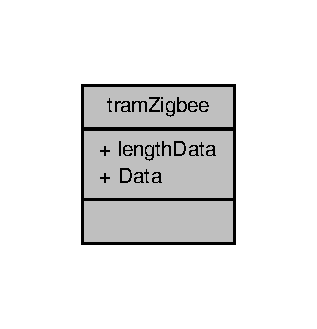
\includegraphics[width=152pt]{structtramZigbee__coll__graph}
\end{center}
\end{figure}
\subsection*{Public Attributes}
\begin{DoxyCompactItemize}
\item 
char \hyperlink{structtramZigbee_a688bc48e9e6da34837d4636d5e60b849}{length\-Data}
\item 
char \hyperlink{structtramZigbee_a3871224e0e052d996b31a4f1d4df51f2}{Data} \mbox{[}72\mbox{]}
\end{DoxyCompactItemize}


\subsection{Detailed Description}


Definition at line 14 of file typdef\-Uart.\-h.



\subsection{Member Data Documentation}
\hypertarget{structtramZigbee_a3871224e0e052d996b31a4f1d4df51f2}{\index{tram\-Zigbee@{tram\-Zigbee}!Data@{Data}}
\index{Data@{Data}!tramZigbee@{tram\-Zigbee}}
\subsubsection[{Data}]{\setlength{\rightskip}{0pt plus 5cm}char tram\-Zigbee\-::\-Data\mbox{[}72\mbox{]}}}\label{structtramZigbee_a3871224e0e052d996b31a4f1d4df51f2}


Definition at line 16 of file typdef\-Uart.\-h.

\hypertarget{structtramZigbee_a688bc48e9e6da34837d4636d5e60b849}{\index{tram\-Zigbee@{tram\-Zigbee}!length\-Data@{length\-Data}}
\index{length\-Data@{length\-Data}!tramZigbee@{tram\-Zigbee}}
\subsubsection[{length\-Data}]{\setlength{\rightskip}{0pt plus 5cm}char tram\-Zigbee\-::length\-Data}}\label{structtramZigbee_a688bc48e9e6da34837d4636d5e60b849}


Definition at line 15 of file typdef\-Uart.\-h.



The documentation for this struct was generated from the following file\-:\begin{DoxyCompactItemize}
\item 
\hyperlink{typdefUart_8h}{typdef\-Uart.\-h}\end{DoxyCompactItemize}

\hypertarget{classUart}{\section{Uart Class Reference}
\label{classUart}\index{Uart@{Uart}}
}


{\ttfamily \#include \char`\"{}uart.\-h\char`\"{}}



Inheritance diagram for Uart\-:\nopagebreak
\begin{figure}[H]
\begin{center}
\leavevmode
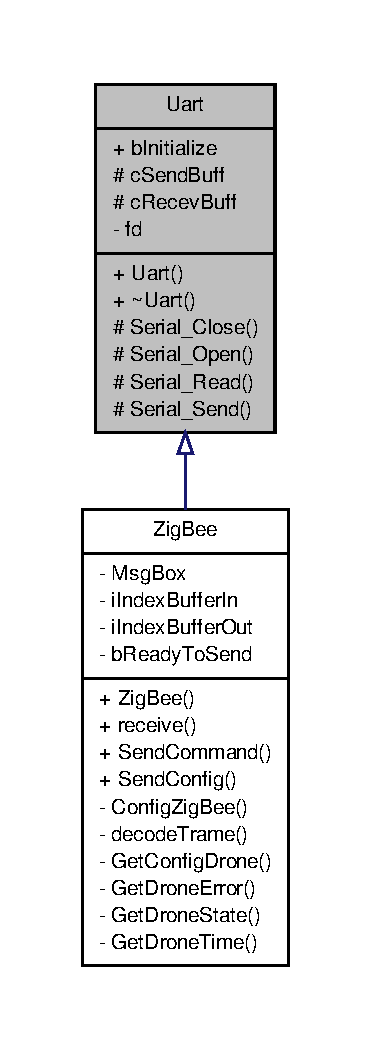
\includegraphics[width=178pt]{classUart__inherit__graph}
\end{center}
\end{figure}


Collaboration diagram for Uart\-:\nopagebreak
\begin{figure}[H]
\begin{center}
\leavevmode
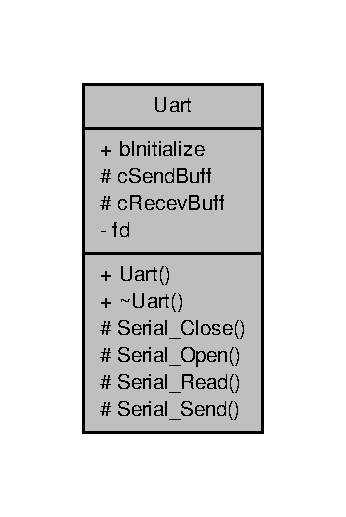
\includegraphics[width=166pt]{classUart__coll__graph}
\end{center}
\end{figure}
\subsection*{Public Member Functions}
\begin{DoxyCompactItemize}
\item 
\hyperlink{classUart_af65a6888b8a623bdc70cfb5c5e8e9957}{Uart} ()
\item 
\hyperlink{classUart_a7160154094413395a23dbaa287dbef3c}{$\sim$\-Uart} ()
\end{DoxyCompactItemize}
\subsection*{Public Attributes}
\begin{DoxyCompactItemize}
\item 
bool \hyperlink{classUart_a082b349fdf73dd9f4e1a2f1a09af28c3}{b\-Initialize}
\end{DoxyCompactItemize}
\subsection*{Protected Member Functions}
\begin{DoxyCompactItemize}
\item 
bool \hyperlink{classUart_ac21470b359f66cc072f80b638258aa18}{Serial\-\_\-\-Close} ()
\item 
bool \hyperlink{classUart_ab41a877a430c87419c524c970d033ee5}{Serial\-\_\-\-Open} (const char $\ast$serial\-\_\-\-Name, speed\-\_\-t baudrate)
\item 
int \hyperlink{classUart_aba195c21510bc9bbab776b961d866e1e}{Serial\-\_\-\-Read} (char $\ast$buff, int len)
\item 
int \hyperlink{classUart_ace4b7eaee7374cac2c91ca627b2a78b6}{Serial\-\_\-\-Send} (char $\ast$string, int len)
\end{DoxyCompactItemize}
\subsection*{Protected Attributes}
\begin{DoxyCompactItemize}
\item 
char \hyperlink{classUart_a41faef9fcb605cc62769abb551f49b1a}{c\-Send\-Buff} \mbox{[}12\mbox{]}
\item 
char \hyperlink{classUart_afe931bc10d90890bce0d9331edb99598}{c\-Recev\-Buff} \mbox{[}12\mbox{]}
\end{DoxyCompactItemize}
\subsection*{Private Attributes}
\begin{DoxyCompactItemize}
\item 
int \hyperlink{classUart_a9beb12dfe4b673ede7b05ec04af0dee8}{fd}
\end{DoxyCompactItemize}


\subsection{Detailed Description}


Definition at line 21 of file uart.\-h.



\subsection{Constructor \& Destructor Documentation}
\hypertarget{classUart_af65a6888b8a623bdc70cfb5c5e8e9957}{\index{Uart@{Uart}!Uart@{Uart}}
\index{Uart@{Uart}!Uart@{Uart}}
\subsubsection[{Uart}]{\setlength{\rightskip}{0pt plus 5cm}Uart\-::\-Uart (
\begin{DoxyParamCaption}
{}
\end{DoxyParamCaption}
)}}\label{classUart_af65a6888b8a623bdc70cfb5c5e8e9957}


Definition at line 5 of file uart.\-cpp.



References b\-Initialize, fd, param\-\_\-\-U\-A\-R\-T\-\_\-\-F\-I\-L\-E, and Serial\-\_\-\-Open().


\begin{DoxyCode}
\{
    tcflush(\hyperlink{classUart_a9beb12dfe4b673ede7b05ec04af0dee8}{fd}, TCIOFLUSH);
    \hyperlink{classUart_a082b349fdf73dd9f4e1a2f1a09af28c3}{bInitialize} = \hyperlink{classUart_ab41a877a430c87419c524c970d033ee5}{Serial\_Open}(\hyperlink{uart_8h_ab24fe93d414e2d2790a5ce8e5503fd7d}{param\_UART\_FILE}
      , B9600);
\}
\end{DoxyCode}
\hypertarget{classUart_a7160154094413395a23dbaa287dbef3c}{\index{Uart@{Uart}!$\sim$\-Uart@{$\sim$\-Uart}}
\index{$\sim$\-Uart@{$\sim$\-Uart}!Uart@{Uart}}
\subsubsection[{$\sim$\-Uart}]{\setlength{\rightskip}{0pt plus 5cm}Uart\-::$\sim$\-Uart (
\begin{DoxyParamCaption}
{}
\end{DoxyParamCaption}
)}}\label{classUart_a7160154094413395a23dbaa287dbef3c}


Definition at line 11 of file uart.\-cpp.



References Serial\-\_\-\-Close().


\begin{DoxyCode}
\{
    \hyperlink{classUart_ac21470b359f66cc072f80b638258aa18}{Serial\_Close}();
\}
\end{DoxyCode}


\subsection{Member Function Documentation}
\hypertarget{classUart_ac21470b359f66cc072f80b638258aa18}{\index{Uart@{Uart}!Serial\-\_\-\-Close@{Serial\-\_\-\-Close}}
\index{Serial\-\_\-\-Close@{Serial\-\_\-\-Close}!Uart@{Uart}}
\subsubsection[{Serial\-\_\-\-Close}]{\setlength{\rightskip}{0pt plus 5cm}bool Uart\-::\-Serial\-\_\-\-Close (
\begin{DoxyParamCaption}
{}
\end{DoxyParamCaption}
)\hspace{0.3cm}{\ttfamily [protected]}}}\label{classUart_ac21470b359f66cc072f80b638258aa18}


Definition at line 61 of file uart.\-cpp.



References fd.



Referenced by $\sim$\-Uart().


\begin{DoxyCode}
\{
        \textcolor{keywordflow}{if}(close (\hyperlink{classUart_a9beb12dfe4b673ede7b05ec04af0dee8}{fd}) < 0)
        \{
            \textcolor{keywordflow}{return} \textcolor{keyword}{false};
                \}
                \textcolor{keywordflow}{else}
            \textcolor{keywordflow}{return} \textcolor{keyword}{true};
\}
\end{DoxyCode}
\hypertarget{classUart_ab41a877a430c87419c524c970d033ee5}{\index{Uart@{Uart}!Serial\-\_\-\-Open@{Serial\-\_\-\-Open}}
\index{Serial\-\_\-\-Open@{Serial\-\_\-\-Open}!Uart@{Uart}}
\subsubsection[{Serial\-\_\-\-Open}]{\setlength{\rightskip}{0pt plus 5cm}bool Uart\-::\-Serial\-\_\-\-Open (
\begin{DoxyParamCaption}
\item[{const char $\ast$}]{serial\-\_\-\-Name, }
\item[{speed\-\_\-t}]{baudrate}
\end{DoxyParamCaption}
)\hspace{0.3cm}{\ttfamily [protected]}}}\label{classUart_ab41a877a430c87419c524c970d033ee5}


Definition at line 16 of file uart.\-cpp.



References fd.



Referenced by Uart().


\begin{DoxyCode}
\{
    \textcolor{keyword}{struct }termios serCfg;

        memset(&serCfg, 0, \textcolor{keyword}{sizeof}(serCfg));

    \textcolor{keywordflow}{if}((\hyperlink{classUart_a9beb12dfe4b673ede7b05ec04af0dee8}{fd} = open(serial\_Name, O\_RDWR | O\_NOCTTY | O\_NDELAY )) < 0) \{
        printf(\textcolor{stringliteral}{"Failed to open serial port"});
        \textcolor{keywordflow}{return} \textcolor{keyword}{false};
        \}
    \textcolor{keywordflow}{else} \textcolor{keywordflow}{if}(tcgetattr(\hyperlink{classUart_a9beb12dfe4b673ede7b05ec04af0dee8}{fd}, &serCfg) != 0) \{
            printf(\textcolor{stringliteral}{"Failed to get configuration"});
            \textcolor{keywordflow}{return} \textcolor{keyword}{false};
    \}

        cfsetispeed(&serCfg, baudrate);
        cfsetospeed(&serCfg, baudrate);
        cfmakeraw(&serCfg);

    \textcolor{keywordflow}{if}(tcsetattr(\hyperlink{classUart_a9beb12dfe4b673ede7b05ec04af0dee8}{fd}, TCSANOW, &serCfg) != 0) \{
        printf(\textcolor{stringliteral}{"Failed to set configuration"});
        \textcolor{keywordflow}{return} \textcolor{keyword}{false};
        \}
    \textcolor{keywordflow}{return} \textcolor{keyword}{true};
\}
\end{DoxyCode}
\hypertarget{classUart_aba195c21510bc9bbab776b961d866e1e}{\index{Uart@{Uart}!Serial\-\_\-\-Read@{Serial\-\_\-\-Read}}
\index{Serial\-\_\-\-Read@{Serial\-\_\-\-Read}!Uart@{Uart}}
\subsubsection[{Serial\-\_\-\-Read}]{\setlength{\rightskip}{0pt plus 5cm}int Uart\-::\-Serial\-\_\-\-Read (
\begin{DoxyParamCaption}
\item[{char $\ast$}]{buff, }
\item[{int}]{len}
\end{DoxyParamCaption}
)\hspace{0.3cm}{\ttfamily [protected]}}}\label{classUart_aba195c21510bc9bbab776b961d866e1e}


Definition at line 51 of file uart.\-cpp.



References b\-Initialize, and fd.



Referenced by Zig\-Bee\-::\-Config\-Zig\-Bee(), and Zig\-Bee\-::receive().


\begin{DoxyCode}
\{
    \textcolor{keywordflow}{if}(\hyperlink{classUart_a082b349fdf73dd9f4e1a2f1a09af28c3}{bInitialize}) \{
        \textcolor{keywordflow}{return} read(\hyperlink{classUart_a9beb12dfe4b673ede7b05ec04af0dee8}{fd}, buff, len);
    \}
    \textcolor{keywordflow}{else} \{
        \textcolor{keywordflow}{return} -1;
    \}
\}
\end{DoxyCode}
\hypertarget{classUart_ace4b7eaee7374cac2c91ca627b2a78b6}{\index{Uart@{Uart}!Serial\-\_\-\-Send@{Serial\-\_\-\-Send}}
\index{Serial\-\_\-\-Send@{Serial\-\_\-\-Send}!Uart@{Uart}}
\subsubsection[{Serial\-\_\-\-Send}]{\setlength{\rightskip}{0pt plus 5cm}int Uart\-::\-Serial\-\_\-\-Send (
\begin{DoxyParamCaption}
\item[{char $\ast$}]{string, }
\item[{int}]{len}
\end{DoxyParamCaption}
)\hspace{0.3cm}{\ttfamily [protected]}}}\label{classUart_ace4b7eaee7374cac2c91ca627b2a78b6}


Definition at line 41 of file uart.\-cpp.



References b\-Initialize, and fd.



Referenced by Zig\-Bee\-::\-Config\-Zig\-Bee(), and Zig\-Bee\-::\-Send\-Command().


\begin{DoxyCode}
\{
    \textcolor{keywordflow}{if}(\hyperlink{classUart_a082b349fdf73dd9f4e1a2f1a09af28c3}{bInitialize}) \{
        \textcolor{keywordflow}{return} write(\hyperlink{classUart_a9beb12dfe4b673ede7b05ec04af0dee8}{fd}, \textcolor{keywordtype}{string},len);
    \}
    \textcolor{keywordflow}{else} \{
        \textcolor{keywordflow}{return} -1;
    \}
\}
\end{DoxyCode}


\subsection{Member Data Documentation}
\hypertarget{classUart_a082b349fdf73dd9f4e1a2f1a09af28c3}{\index{Uart@{Uart}!b\-Initialize@{b\-Initialize}}
\index{b\-Initialize@{b\-Initialize}!Uart@{Uart}}
\subsubsection[{b\-Initialize}]{\setlength{\rightskip}{0pt plus 5cm}bool Uart\-::b\-Initialize}}\label{classUart_a082b349fdf73dd9f4e1a2f1a09af28c3}


Definition at line 28 of file uart.\-h.



Referenced by Q\-Base\-::\-Q\-Base(), Serial\-\_\-\-Read(), Serial\-\_\-\-Send(), Uart(), and Zig\-Bee\-::\-Zig\-Bee().

\hypertarget{classUart_afe931bc10d90890bce0d9331edb99598}{\index{Uart@{Uart}!c\-Recev\-Buff@{c\-Recev\-Buff}}
\index{c\-Recev\-Buff@{c\-Recev\-Buff}!Uart@{Uart}}
\subsubsection[{c\-Recev\-Buff}]{\setlength{\rightskip}{0pt plus 5cm}char Uart\-::c\-Recev\-Buff\mbox{[}12\mbox{]}\hspace{0.3cm}{\ttfamily [protected]}}}\label{classUart_afe931bc10d90890bce0d9331edb99598}


Definition at line 36 of file uart.\-h.



Referenced by Zig\-Bee\-::\-Config\-Zig\-Bee().

\hypertarget{classUart_a41faef9fcb605cc62769abb551f49b1a}{\index{Uart@{Uart}!c\-Send\-Buff@{c\-Send\-Buff}}
\index{c\-Send\-Buff@{c\-Send\-Buff}!Uart@{Uart}}
\subsubsection[{c\-Send\-Buff}]{\setlength{\rightskip}{0pt plus 5cm}char Uart\-::c\-Send\-Buff\mbox{[}12\mbox{]}\hspace{0.3cm}{\ttfamily [protected]}}}\label{classUart_a41faef9fcb605cc62769abb551f49b1a}


Definition at line 35 of file uart.\-h.

\hypertarget{classUart_a9beb12dfe4b673ede7b05ec04af0dee8}{\index{Uart@{Uart}!fd@{fd}}
\index{fd@{fd}!Uart@{Uart}}
\subsubsection[{fd}]{\setlength{\rightskip}{0pt plus 5cm}int Uart\-::fd\hspace{0.3cm}{\ttfamily [private]}}}\label{classUart_a9beb12dfe4b673ede7b05ec04af0dee8}


Definition at line 39 of file uart.\-h.



Referenced by Serial\-\_\-\-Close(), Serial\-\_\-\-Open(), Serial\-\_\-\-Read(), Serial\-\_\-\-Send(), and Uart().



The documentation for this class was generated from the following files\-:\begin{DoxyCompactItemize}
\item 
\hyperlink{uart_8h}{uart.\-h}\item 
\hyperlink{uart_8cpp}{uart.\-cpp}\end{DoxyCompactItemize}

\hypertarget{classZigBee}{\section{Zig\-Bee Class Reference}
\label{classZigBee}\index{Zig\-Bee@{Zig\-Bee}}
}


{\ttfamily \#include \char`\"{}zigbee.\-h\char`\"{}}



Inheritance diagram for Zig\-Bee\-:\nopagebreak
\begin{figure}[H]
\begin{center}
\leavevmode
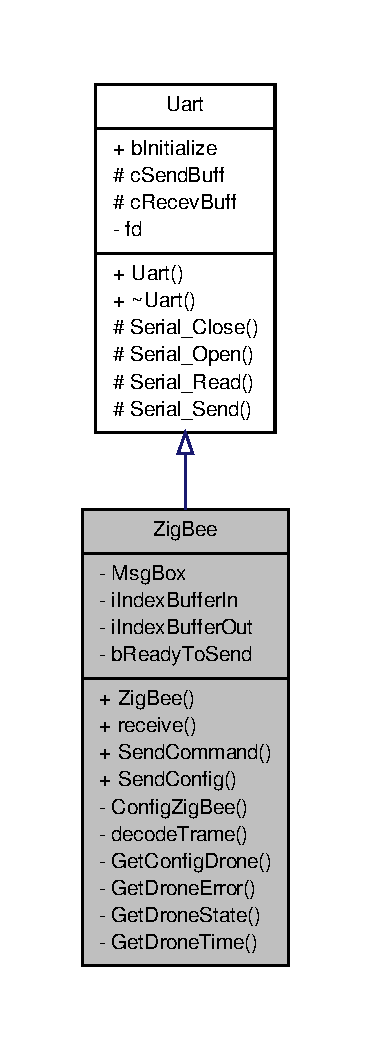
\includegraphics[width=178pt]{classZigBee__inherit__graph}
\end{center}
\end{figure}


Collaboration diagram for Zig\-Bee\-:\nopagebreak
\begin{figure}[H]
\begin{center}
\leavevmode
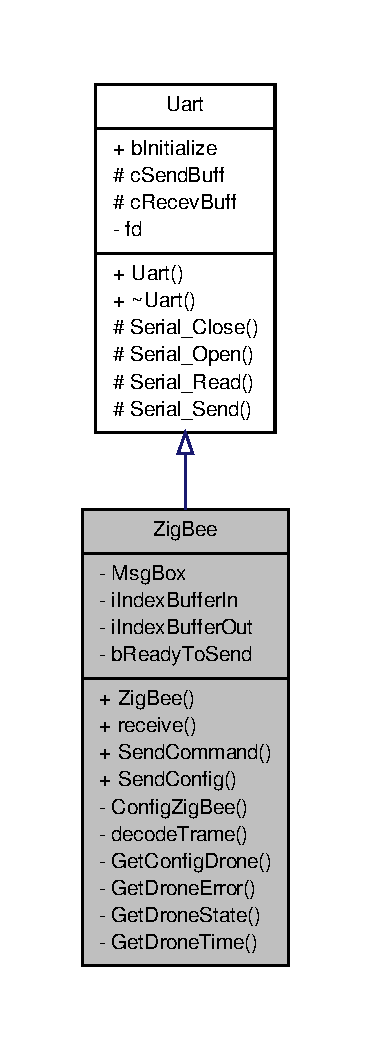
\includegraphics[width=178pt]{classZigBee__coll__graph}
\end{center}
\end{figure}
\subsection*{Public Member Functions}
\begin{DoxyCompactItemize}
\item 
\hyperlink{classZigBee_a488ea980dd12ecd0d02be341f7f6af1b}{Zig\-Bee} ()
\item 
void \hyperlink{classZigBee_a0852f85771d48df17a6256edcd91bece}{receive} ()
\item 
void \hyperlink{classZigBee_a6b69e04be626400b5b245fa1b56f0810}{Send\-Command} ()
\item 
void \hyperlink{classZigBee_aef177ea29c57953e74ddcd8bb356fe2f}{Send\-Config} ()
\end{DoxyCompactItemize}
\subsection*{Private Member Functions}
\begin{DoxyCompactItemize}
\item 
bool \hyperlink{classZigBee_a318ed8b8b67393a603c4bfcf0dd0524f}{Config\-Zig\-Bee} ()
\item 
void \hyperlink{classZigBee_a8967d2ce7d04ce2d267654975e5bc87c}{decode\-Trame} ()
\item 
void \hyperlink{classZigBee_a1817781f9b8e805bdd4eba25498714fe}{Get\-Config\-Drone} (\hyperlink{typdefUart_8h_a435d1572bf3f880d55459d9805097f62}{uint32\-\_\-t} $\ast$param)
\item 
void \hyperlink{classZigBee_ac4ea5e99c087a7e536d97a41ef8145d2}{Get\-Drone\-Error} (\hyperlink{typdefUart_8h_aad4124e5a34e185d704fe88506ecf352}{drone\-Error} $\ast$param)
\item 
void \hyperlink{classZigBee_a246506a3d990d052a37a4d816b88f3e6}{Get\-Drone\-State} (\hyperlink{typdefUart_8h_aac9034800b5ef8e755ade03d164e3b6c}{drone\-Flt\-State} $\ast$param)
\item 
void \hyperlink{classZigBee_a65751fbcd303e5c8e5ff63d69f5eba35}{Get\-Drone\-Time} (\hyperlink{typdefUart_8h_ae9fa5e001303f1be1c0294f26cde8caf}{port\-Tick\-Type} $\ast$param)
\end{DoxyCompactItemize}
\subsection*{Private Attributes}
\begin{DoxyCompactItemize}
\item 
Q\-Message\-Box \hyperlink{classZigBee_a7048223c8f5546e3614641cba1062357}{Msg\-Box}
\item 
int \hyperlink{classZigBee_a2b6ec705974d8db622f3eb00efeb9ad8}{i\-Index\-Buffer\-In}
\item 
int \hyperlink{classZigBee_aa510069113962d7a107f27c4d798d08c}{i\-Index\-Buffer\-Out}
\item 
bool \hyperlink{classZigBee_ac954bdd2f3b1c5bcfe11563765f10878}{b\-Ready\-To\-Send}
\end{DoxyCompactItemize}
\subsection*{Additional Inherited Members}


\subsection{Detailed Description}


Definition at line 13 of file zigbee.\-h.



\subsection{Constructor \& Destructor Documentation}
\hypertarget{classZigBee_a488ea980dd12ecd0d02be341f7f6af1b}{\index{Zig\-Bee@{Zig\-Bee}!Zig\-Bee@{Zig\-Bee}}
\index{Zig\-Bee@{Zig\-Bee}!ZigBee@{Zig\-Bee}}
\subsubsection[{Zig\-Bee}]{\setlength{\rightskip}{0pt plus 5cm}Zig\-Bee\-::\-Zig\-Bee (
\begin{DoxyParamCaption}
{}
\end{DoxyParamCaption}
)\hspace{0.3cm}{\ttfamily [explicit]}}}\label{classZigBee_a488ea980dd12ecd0d02be341f7f6af1b}


Definition at line 3 of file zigbee.\-cpp.



References Uart\-::b\-Initialize, b\-Ready\-To\-Send, Config\-Zig\-Bee(), D\-R\-N\-\_\-\-E\-R\-R\-\_\-\-N\-O\-N\-E, and S\-T\-A\-T\-E\-\_\-\-S\-T\-A\-R\-T\-I\-N\-G.


\begin{DoxyCode}
\{
    \textcolor{keywordflow}{if}(\hyperlink{classUart_a082b349fdf73dd9f4e1a2f1a09af28c3}{bInitialize}) \{

        \hyperlink{classUart_a082b349fdf73dd9f4e1a2f1a09af28c3}{bInitialize} = \hyperlink{classZigBee_a318ed8b8b67393a603c4bfcf0dd0524f}{ConfigZigBee}();
        st\_CommandDrone.cTransX = 0;
        st\_CommandDrone.cTransY = 0;
        st\_CommandDrone.cTransZ = 0;
        st\_CommandDrone.cRotZ = 0;
        st\_DataIMU.xUpdateTime = 0;
        st\_DataGPS.xUpdateTime = 0;
        st\_DroneState.eErrorMask = \hyperlink{typdefUart_8h_aad4124e5a34e185d704fe88506ecf352a4eb8e22beceecc6e83a76fc46f56e03a}{DRN\_ERR\_NONE};
        st\_DroneState.eFltState = \hyperlink{typdefUart_8h_aac9034800b5ef8e755ade03d164e3b6caa5f51c4eb8c8eec3b16b058c5e29a037}{STATE\_STARTING};
        \hyperlink{classZigBee_ac954bdd2f3b1c5bcfe11563765f10878}{bReadyToSend} = \textcolor{keyword}{false};
    \}
    \textcolor{keywordflow}{else} \{
        \textcolor{comment}{//Erreur d'init UART}
    \}
\}
\end{DoxyCode}


\subsection{Member Function Documentation}
\hypertarget{classZigBee_a318ed8b8b67393a603c4bfcf0dd0524f}{\index{Zig\-Bee@{Zig\-Bee}!Config\-Zig\-Bee@{Config\-Zig\-Bee}}
\index{Config\-Zig\-Bee@{Config\-Zig\-Bee}!ZigBee@{Zig\-Bee}}
\subsubsection[{Config\-Zig\-Bee}]{\setlength{\rightskip}{0pt plus 5cm}bool Zig\-Bee\-::\-Config\-Zig\-Bee (
\begin{DoxyParamCaption}
{}
\end{DoxyParamCaption}
)\hspace{0.3cm}{\ttfamily [private]}}}\label{classZigBee_a318ed8b8b67393a603c4bfcf0dd0524f}


Definition at line 23 of file zigbee.\-cpp.



References Uart\-::c\-Recev\-Buff, H\-I\-S\-T\-O\-R\-Y\-\_\-\-D\-E\-S\-T\-\_\-\-H, param\-\_\-\-A\-D\-R\-E\-S\-S\-E\-\_\-\-D\-E\-S\-T\-\_\-\-H, param\-\_\-\-A\-D\-R\-E\-S\-S\-E\-\_\-\-D\-E\-S\-T\-\_\-\-L, param\-\_\-\-A\-D\-R\-E\-S\-S\-E\-\_\-\-E\-M\-E\-T\-\_\-\-H, param\-\_\-\-A\-D\-R\-E\-S\-S\-E\-\_\-\-E\-M\-E\-T\-\_\-\-L, param\-\_\-\-E\-N\-T\-R\-E\-\_\-\-C\-O\-N\-F\-I\-G, param\-\_\-\-Q\-U\-I\-T\-E\-\_\-\-C\-O\-N\-F\-I\-G, Uart\-::\-Serial\-\_\-\-Read(), and Uart\-::\-Serial\-\_\-\-Send().



Referenced by Zig\-Bee().


\begin{DoxyCode}
\{
    \hyperlink{classUart_ace4b7eaee7374cac2c91ca627b2a78b6}{Serial\_Send}(\hyperlink{uart_8h_af89774268ea3d3837342a1698e105883}{param\_ENTRE\_CONFIG}, 3);

    \hyperlink{classUart_aba195c21510bc9bbab776b961d866e1e}{Serial\_Read}(\hyperlink{classUart_afe931bc10d90890bce0d9331edb99598}{cRecevBuff}, 2);      \textcolor{comment}{//Reçoit la
       confirmation}

    \textcolor{keywordflow}{if}(\hyperlink{classUart_afe931bc10d90890bce0d9331edb99598}{cRecevBuff}[0] != \textcolor{charliteral}{'o'} || \hyperlink{classUart_afe931bc10d90890bce0d9331edb99598}{cRecevBuff}[1] != \textcolor{charliteral}{'k'}) \{
        \textcolor{keywordflow}{return} \textcolor{keyword}{false};               \textcolor{comment}{//Si pas de confirmation, on quite}
    \}

    \hyperlink{classUart_ace4b7eaee7374cac2c91ca627b2a78b6}{Serial\_Send}(\hyperlink{uart_8h_a5eb04239c6384873a45b0c4f43aaa864}{param\_ADRESSE\_EMET\_H}, 4);       
            \textcolor{comment}{//Demande l'adresse de l'émetteur (MSBs)}

    \hyperlink{classUart_aba195c21510bc9bbab776b961d866e1e}{Serial\_Read}(\hyperlink{classUart_afe931bc10d90890bce0d9331edb99598}{cRecevBuff}, 4);

    printf(\textcolor{stringliteral}{"adresse du module : %X %X %X %X "},\hyperlink{classUart_afe931bc10d90890bce0d9331edb99598}{cRecevBuff}[0],\hyperlink{classUart_afe931bc10d90890bce0d9331edb99598}{
      cRecevBuff}[1],\hyperlink{classUart_afe931bc10d90890bce0d9331edb99598}{cRecevBuff}[2],\hyperlink{classUart_afe931bc10d90890bce0d9331edb99598}{cRecevBuff}[3]);

    \hyperlink{classUart_ace4b7eaee7374cac2c91ca627b2a78b6}{Serial\_Send}(\hyperlink{uart_8h_ac12bfbd9bb75329241513b728f667963}{param\_ADRESSE\_EMET\_L}, 4);       
            \textcolor{comment}{//Demande l'adresse de l'émetteur (LSBs)}

    \hyperlink{classUart_aba195c21510bc9bbab776b961d866e1e}{Serial\_Read}(\hyperlink{classUart_afe931bc10d90890bce0d9331edb99598}{cRecevBuff}, 4);

    printf(\textcolor{stringliteral}{"%X %X %X %X\(\backslash\)n"},\hyperlink{classUart_afe931bc10d90890bce0d9331edb99598}{cRecevBuff}[0],\hyperlink{classUart_afe931bc10d90890bce0d9331edb99598}{cRecevBuff}[1],
      \hyperlink{classUart_afe931bc10d90890bce0d9331edb99598}{cRecevBuff}[2],\hyperlink{classUart_afe931bc10d90890bce0d9331edb99598}{cRecevBuff}[3]);

    \hyperlink{classUart_ace4b7eaee7374cac2c91ca627b2a78b6}{Serial\_Send}(\hyperlink{uart_8h_a54593750162c64711790d32ae7deb6a0}{param\_ADRESSE\_DEST\_H}, 4);       
            \textcolor{comment}{//Demande l'adresse du recepteur (MSBs)}

    \hyperlink{classUart_aba195c21510bc9bbab776b961d866e1e}{Serial\_Read}(\hyperlink{classUart_afe931bc10d90890bce0d9331edb99598}{cRecevBuff}, 4);

    \textcolor{keywordflow}{if}(strncmp(\hyperlink{classUart_afe931bc10d90890bce0d9331edb99598}{cRecevBuff}, \hyperlink{uart_8h_a2d0c6f9659fde77efee0b205d121ff46}{HISTORY\_DEST\_H}, 4) != 0) \{
\textcolor{comment}{//        return false;}
        \textcolor{comment}{//Si différente, on tape dedans...}
    \}

    \hyperlink{classUart_ace4b7eaee7374cac2c91ca627b2a78b6}{Serial\_Send}(\hyperlink{uart_8h_ab612303ad75cf1a97d2a79ea2760561b}{param\_ADRESSE\_DEST\_L}, 4);       
            \textcolor{comment}{//Demande l'adresse du recepteur (LSBs)}

    \hyperlink{classUart_aba195c21510bc9bbab776b961d866e1e}{Serial\_Read}(\hyperlink{classUart_afe931bc10d90890bce0d9331edb99598}{cRecevBuff}, 4);

    \textcolor{keywordflow}{if}(strncmp(\hyperlink{classUart_afe931bc10d90890bce0d9331edb99598}{cRecevBuff}, \hyperlink{uart_8h_a2d0c6f9659fde77efee0b205d121ff46}{HISTORY\_DEST\_H}, 4) != 0) \{
\textcolor{comment}{//        return false;}
        \textcolor{comment}{//Si différente, on tape dedans...}
    \}

    \hyperlink{classUart_ace4b7eaee7374cac2c91ca627b2a78b6}{Serial\_Send}(\hyperlink{uart_8h_ab8d053e00fdf4476be4730d5390bfd73}{param\_QUITE\_CONFIG}, 4);           
        \textcolor{comment}{//Quite la Config}

    \hyperlink{classUart_aba195c21510bc9bbab776b961d866e1e}{Serial\_Read}(\hyperlink{classUart_afe931bc10d90890bce0d9331edb99598}{cRecevBuff}, 2);      \textcolor{comment}{//Reçoit la
       confirmation}

    \textcolor{keywordflow}{if}(\hyperlink{classUart_afe931bc10d90890bce0d9331edb99598}{cRecevBuff}[0] != \textcolor{charliteral}{'o'} || \hyperlink{classUart_afe931bc10d90890bce0d9331edb99598}{cRecevBuff}[1] != \textcolor{charliteral}{'k'}) \{
        \textcolor{keywordflow}{return} \textcolor{keyword}{false};               \textcolor{comment}{//Si pas de confirmation, on quite}
    \}

    \textcolor{keywordflow}{return} \textcolor{keyword}{true};
\}
\end{DoxyCode}
\hypertarget{classZigBee_a8967d2ce7d04ce2d267654975e5bc87c}{\index{Zig\-Bee@{Zig\-Bee}!decode\-Trame@{decode\-Trame}}
\index{decode\-Trame@{decode\-Trame}!ZigBee@{Zig\-Bee}}
\subsubsection[{decode\-Trame}]{\setlength{\rightskip}{0pt plus 5cm}void Zig\-Bee\-::decode\-Trame (
\begin{DoxyParamCaption}
{}
\end{DoxyParamCaption}
)\hspace{0.3cm}{\ttfamily [private]}}}\label{classZigBee_a8967d2ce7d04ce2d267654975e5bc87c}


Definition at line 128 of file zigbee.\-cpp.



References b\-Ready\-To\-Send, Get\-Config\-Drone(), Get\-Drone\-Error(), Get\-Drone\-State(), Get\-Drone\-Time(), i\-Index\-Buffer\-In, P\-A\-R\-A\-M\-\_\-\-D\-R\-O\-N\-E\-\_\-\-C\-O\-N\-F\-I\-G\-\_\-ul\-Crit\-Battery\-Lvl, P\-A\-R\-A\-M\-\_\-\-D\-R\-O\-N\-E\-\_\-\-C\-O\-N\-F\-I\-G\-\_\-ul\-Crit\-Obstacle\-Dist, P\-A\-R\-A\-M\-\_\-\-D\-R\-O\-N\-E\-\_\-\-C\-O\-N\-F\-I\-G\-\_\-ul\-Crit\-Zigbee\-Signal\-Lvl, P\-A\-R\-A\-M\-\_\-\-D\-R\-O\-N\-E\-\_\-\-C\-O\-N\-F\-I\-G\-\_\-ul\-Max\-Angle, P\-A\-R\-A\-M\-\_\-\-D\-R\-O\-N\-E\-\_\-\-C\-O\-N\-F\-I\-G\-\_\-ul\-Min\-Altitude, P\-A\-R\-A\-M\-\_\-\-D\-R\-O\-N\-E\-\_\-\-C\-O\-N\-F\-I\-G\-\_\-ul\-Takeoff\-Altitude, P\-A\-R\-A\-M\-\_\-\-D\-R\-O\-N\-E\-\_\-\-C\-O\-N\-F\-I\-G\-\_\-x\-Battery\-Monitoring\-Period, P\-A\-R\-A\-M\-\_\-\-D\-R\-O\-N\-E\-\_\-\-C\-O\-N\-F\-I\-G\-\_\-x\-Battery\-Timeout, P\-A\-R\-A\-M\-\_\-\-D\-R\-O\-N\-E\-\_\-\-C\-O\-N\-F\-I\-G\-\_\-x\-Detect\-Obstacle\-Period, P\-A\-R\-A\-M\-\_\-\-D\-R\-O\-N\-E\-\_\-\-C\-O\-N\-F\-I\-G\-\_\-x\-Flight\-Ctrl\-Period, P\-A\-R\-A\-M\-\_\-\-D\-R\-O\-N\-E\-\_\-\-C\-O\-N\-F\-I\-G\-\_\-x\-G\-P\-S\-Receive\-Period, P\-A\-R\-A\-M\-\_\-\-D\-R\-O\-N\-E\-\_\-\-C\-O\-N\-F\-I\-G\-\_\-x\-G\-P\-S\-Timeout, P\-A\-R\-A\-M\-\_\-\-D\-R\-O\-N\-E\-\_\-\-C\-O\-N\-F\-I\-G\-\_\-x\-I\-M\-U\-Data\-Timeout, P\-A\-R\-A\-M\-\_\-\-D\-R\-O\-N\-E\-\_\-\-C\-O\-N\-F\-I\-G\-\_\-x\-Telemeter\-Timeout, P\-A\-R\-A\-M\-\_\-\-D\-R\-O\-N\-E\-\_\-\-C\-O\-N\-F\-I\-G\-\_\-x\-Video\-Toggle\-Period, P\-A\-R\-A\-M\-\_\-\-D\-R\-O\-N\-E\-\_\-\-C\-O\-N\-F\-I\-G\-\_\-x\-Zigbee\-Cmd\-Timeout, P\-A\-R\-A\-M\-\_\-\-D\-R\-O\-N\-E\-\_\-\-C\-O\-N\-F\-I\-G\-\_\-x\-Zigbee\-Receive\-Period, P\-A\-R\-A\-M\-\_\-\-D\-R\-O\-N\-E\-\_\-\-C\-O\-N\-F\-I\-G\-\_\-x\-Zigbee\-Receive\-Timeout, P\-A\-R\-A\-M\-\_\-\-D\-R\-O\-N\-E\-\_\-\-E\-R\-R\-O\-R, P\-A\-R\-A\-M\-\_\-\-F\-L\-Y\-\_\-\-S\-T\-A\-T\-E, P\-A\-R\-A\-M\-\_\-\-G\-P\-S\-\_\-x\-Update\-Time, P\-A\-R\-A\-M\-\_\-\-I\-M\-U\-\_\-x\-Update\-Time, and S\-T\-A\-T\-E\-\_\-\-S\-T\-A\-R\-T\-I\-N\-G.



Referenced by receive().


\begin{DoxyCode}
\{
    \hyperlink{classZigBee_a2b6ec705974d8db622f3eb00efeb9ad8}{iIndexBufferIn} = 0;

    \textcolor{keywordflow}{for}(\textcolor{keywordtype}{int} i = 0 ; i < st\_BufferIn.lengthData ; i++) \{

        \textcolor{keywordflow}{switch}(st\_BufferIn.Data[\hyperlink{classZigBee_a2b6ec705974d8db622f3eb00efeb9ad8}{iIndexBufferIn}++]) \{

        \textcolor{keywordflow}{case} \hyperlink{typdefUart_8h_a7fdf1e7bfbebe0c7a2eb84a10e069632a7828400a62571bb441a0216f1c2e29be}{PARAM\_DRONE\_CONFIG\_ulMaxAngle}:
            \hyperlink{classZigBee_a1817781f9b8e805bdd4eba25498714fe}{GetConfigDrone}(&(st\_droneConfig.ulMaxAngle));
            \textcolor{keywordflow}{break};
        \textcolor{keywordflow}{case} \hyperlink{typdefUart_8h_a7fdf1e7bfbebe0c7a2eb84a10e069632af954ea9792a880b2593da24e0214708f}{PARAM\_DRONE\_CONFIG\_ulTakeoffAltitude}
      :
            \hyperlink{classZigBee_a1817781f9b8e805bdd4eba25498714fe}{GetConfigDrone}(&(st\_droneConfig.ulTakeoffAltitude));
            \textcolor{keywordflow}{break};
        \textcolor{keywordflow}{case} \hyperlink{typdefUart_8h_a7fdf1e7bfbebe0c7a2eb84a10e069632a516ded0a007275ce22b40cba97734484}{PARAM\_DRONE\_CONFIG\_ulMinAltitude}:
            \hyperlink{classZigBee_a1817781f9b8e805bdd4eba25498714fe}{GetConfigDrone}(&(st\_droneConfig.ulMinAltitude));
            \textcolor{keywordflow}{break};
        \textcolor{keywordflow}{case} \hyperlink{typdefUart_8h_a7fdf1e7bfbebe0c7a2eb84a10e069632a212c640074147bd9d0d63888d538d256}{PARAM\_DRONE\_CONFIG\_ulCritBatteryLvl}
      :
            \hyperlink{classZigBee_a1817781f9b8e805bdd4eba25498714fe}{GetConfigDrone}(&(st\_droneConfig.ulCritBatteryLvl));
            \textcolor{keywordflow}{break};
        \textcolor{keywordflow}{case} \hyperlink{typdefUart_8h_a7fdf1e7bfbebe0c7a2eb84a10e069632adc16eed85f98b926f829decb1e7f3175}{PARAM\_DRONE\_CONFIG\_ulCritObstacleDist}
      :
            \hyperlink{classZigBee_a1817781f9b8e805bdd4eba25498714fe}{GetConfigDrone}(&(st\_droneConfig.ulCritObstacleDist));
            \textcolor{keywordflow}{break};
        \textcolor{keywordflow}{case} \hyperlink{typdefUart_8h_a7fdf1e7bfbebe0c7a2eb84a10e069632a91adcfa9ba7373cb5e94cb7dad749286}{PARAM\_DRONE\_CONFIG\_ulCritZigbeeSignalLvl}
      :
            \hyperlink{classZigBee_a1817781f9b8e805bdd4eba25498714fe}{GetConfigDrone}(&(st\_droneConfig.ulCritZigbeeSignalLvl
      ));
            \textcolor{keywordflow}{break};
        \textcolor{keywordflow}{case} \hyperlink{typdefUart_8h_a7fdf1e7bfbebe0c7a2eb84a10e069632adaafa83d8768d26374d1cca8f3c4914d}{PARAM\_DRONE\_CONFIG\_xBatteryMonitoringPeriod}
      :
            \hyperlink{classZigBee_a1817781f9b8e805bdd4eba25498714fe}{GetConfigDrone}(&(st\_droneConfig.
      xBatteryMonitoringPeriod));
            \textcolor{keywordflow}{break};
        \textcolor{keywordflow}{case} \hyperlink{typdefUart_8h_a7fdf1e7bfbebe0c7a2eb84a10e069632a70d207333012bb820cb3576f3fad9048}{PARAM\_DRONE\_CONFIG\_xDetectObstaclePeriod}
      :
            \hyperlink{classZigBee_a1817781f9b8e805bdd4eba25498714fe}{GetConfigDrone}(&(st\_droneConfig.xDetectObstaclePeriod
      ));
            \textcolor{keywordflow}{break};
        \textcolor{keywordflow}{case} \hyperlink{typdefUart_8h_a7fdf1e7bfbebe0c7a2eb84a10e069632a5c305ec532822ca3aa2ff74d0052f757}{PARAM\_DRONE\_CONFIG\_xZigbeeReceivePeriod}
      :
            \hyperlink{classZigBee_a1817781f9b8e805bdd4eba25498714fe}{GetConfigDrone}(&(st\_droneConfig.xZigbeeReceivePeriod)
      );
            \textcolor{keywordflow}{break};
        \textcolor{keywordflow}{case} \hyperlink{typdefUart_8h_a7fdf1e7bfbebe0c7a2eb84a10e069632a22871458b110498e27a8b6244d14fd4e}{PARAM\_DRONE\_CONFIG\_xFlightCtrlPeriod}
      :
            \hyperlink{classZigBee_a1817781f9b8e805bdd4eba25498714fe}{GetConfigDrone}(&(st\_droneConfig.xFlightCtrlPeriod));
            \textcolor{keywordflow}{break};
        \textcolor{keywordflow}{case} \hyperlink{typdefUart_8h_a7fdf1e7bfbebe0c7a2eb84a10e069632a80df4e54f488c528a0af260bf4287bcb}{PARAM\_DRONE\_CONFIG\_xGPSReceivePeriod}
      :
            \hyperlink{classZigBee_a1817781f9b8e805bdd4eba25498714fe}{GetConfigDrone}(&(st\_droneConfig.xGPSReceivePeriod));
            \textcolor{keywordflow}{break};
        \textcolor{keywordflow}{case} \hyperlink{typdefUart_8h_a7fdf1e7bfbebe0c7a2eb84a10e069632a590b78e1b29c0c8dcdf6d2dc869e43aa}{PARAM\_DRONE\_CONFIG\_xVideoTogglePeriod}
      :
            \hyperlink{classZigBee_a1817781f9b8e805bdd4eba25498714fe}{GetConfigDrone}(&(st\_droneConfig.xVideoTogglePeriod));
            \textcolor{keywordflow}{break};
        \textcolor{keywordflow}{case} \hyperlink{typdefUart_8h_a7fdf1e7bfbebe0c7a2eb84a10e069632a8bd205ac7401d53092ff7ffc98e754aa}{PARAM\_DRONE\_CONFIG\_xIMUDataTimeout}
      :
            st\_droneConfig.xIMUDataTimeout = st\_BufferIn.Data[\hyperlink{classZigBee_a2b6ec705974d8db622f3eb00efeb9ad8}{iIndexBufferIn}
      ++];
            \textcolor{keywordflow}{break};
        \textcolor{keywordflow}{case} \hyperlink{typdefUart_8h_a7fdf1e7bfbebe0c7a2eb84a10e069632afaa7777e435be6b471009c6cdf74c948}{PARAM\_DRONE\_CONFIG\_xZigbeeCmdTimeout}
      :
            st\_droneConfig.xZigbeeCmdTimeout = st\_BufferIn.Data[\hyperlink{classZigBee_a2b6ec705974d8db622f3eb00efeb9ad8}{iIndexBufferIn}
      ++];
            \textcolor{keywordflow}{break};
        \textcolor{keywordflow}{case} \hyperlink{typdefUart_8h_a7fdf1e7bfbebe0c7a2eb84a10e069632af2f4da476de6fc43e2118826e9e8bc9b}{PARAM\_DRONE\_CONFIG\_xZigbeeReceiveTimeout}
      :
            st\_droneConfig.xZigbeeReceiveTimeout = st\_BufferIn.Data[
      \hyperlink{classZigBee_a2b6ec705974d8db622f3eb00efeb9ad8}{iIndexBufferIn}++];
            \textcolor{keywordflow}{break};
        \textcolor{keywordflow}{case} \hyperlink{typdefUart_8h_a7fdf1e7bfbebe0c7a2eb84a10e069632aa01da571181efda4755ff66c627d007e}{PARAM\_DRONE\_CONFIG\_xTelemeterTimeout}
      :
            st\_droneConfig.xTelemeterTimeout = st\_BufferIn.Data[\hyperlink{classZigBee_a2b6ec705974d8db622f3eb00efeb9ad8}{iIndexBufferIn}
      ++];
            \textcolor{keywordflow}{break};
        \textcolor{keywordflow}{case} \hyperlink{typdefUart_8h_a7fdf1e7bfbebe0c7a2eb84a10e069632a1298f95dd257a888bde3262a86c4d136}{PARAM\_DRONE\_CONFIG\_xBatteryTimeout}
      :
            st\_droneConfig.xBatteryTimeout = st\_BufferIn.Data[\hyperlink{classZigBee_a2b6ec705974d8db622f3eb00efeb9ad8}{iIndexBufferIn}
      ++];
            \textcolor{keywordflow}{break};
        \textcolor{keywordflow}{case} \hyperlink{typdefUart_8h_a7fdf1e7bfbebe0c7a2eb84a10e069632a9cd65980217626ee680a9055e78d4131}{PARAM\_DRONE\_CONFIG\_xGPSTimeout}:
            st\_droneConfig.xGPSTimeout = st\_BufferIn.Data[\hyperlink{classZigBee_a2b6ec705974d8db622f3eb00efeb9ad8}{iIndexBufferIn}
      ++];
            \textcolor{comment}{//printf("\(\backslash\)n%d\(\backslash\)n",st\_droneConfig.xGPSTimeout);}
            \textcolor{keywordflow}{break};
        \textcolor{keywordflow}{case} \hyperlink{typdefUart_8h_a7fdf1e7bfbebe0c7a2eb84a10e069632a01acce445241211e5ef11328c1b8d1e2}{PARAM\_DRONE\_ERROR}:
            \hyperlink{classZigBee_ac4ea5e99c087a7e536d97a41ef8145d2}{GetDroneError}(&(st\_DroneState.eErrorMask));
            \textcolor{comment}{//ERREUR A TRAITER?}
            \textcolor{comment}{//Ici, si erreur mineur-> on demande si elle doit être ignoré}
                                   \textcolor{comment}{// et on stock pour la prochaine émission}
            \textcolor{keywordflow}{break};
        \textcolor{keywordflow}{case} \hyperlink{typdefUart_8h_a7fdf1e7bfbebe0c7a2eb84a10e069632a8f2ad857311b305a40e6294736196f47}{PARAM\_FLY\_STATE}:
            \hyperlink{classZigBee_a246506a3d990d052a37a4d816b88f3e6}{GetDroneState}(&(st\_DroneState.eFltState));
            \textcolor{keywordflow}{if}(st\_DroneState.eFltState == \hyperlink{typdefUart_8h_aac9034800b5ef8e755ade03d164e3b6caa5f51c4eb8c8eec3b16b058c5e29a037}{STATE\_STARTING})
                \hyperlink{classZigBee_ac954bdd2f3b1c5bcfe11563765f10878}{bReadyToSend} = \textcolor{keyword}{false};
            \textcolor{keywordflow}{break};
        \textcolor{keywordflow}{case} \hyperlink{typdefUart_8h_a7fdf1e7bfbebe0c7a2eb84a10e069632aba9ba51d13875fc28dbcb7aefb4706b2}{PARAM\_IMU\_xUpdateTime}:
            \hyperlink{classZigBee_a65751fbcd303e5c8e5ff63d69f5eba35}{GetDroneTime}(&(st\_DataIMU.xUpdateTime));
            \textcolor{keywordflow}{break};
        \textcolor{keywordflow}{case} \hyperlink{typdefUart_8h_a7fdf1e7bfbebe0c7a2eb84a10e069632af3fc4126f4c3a7540f615932cf7b6144}{PARAM\_GPS\_xUpdateTime}:
            \hyperlink{classZigBee_a65751fbcd303e5c8e5ff63d69f5eba35}{GetDroneTime}(&(st\_DataGPS.xUpdateTime));
            \textcolor{keywordflow}{break};
        \textcolor{keywordflow}{default}:
            \textcolor{keywordflow}{break};
        \}
    \}
\}
\end{DoxyCode}
\hypertarget{classZigBee_a1817781f9b8e805bdd4eba25498714fe}{\index{Zig\-Bee@{Zig\-Bee}!Get\-Config\-Drone@{Get\-Config\-Drone}}
\index{Get\-Config\-Drone@{Get\-Config\-Drone}!ZigBee@{Zig\-Bee}}
\subsubsection[{Get\-Config\-Drone}]{\setlength{\rightskip}{0pt plus 5cm}void Zig\-Bee\-::\-Get\-Config\-Drone (
\begin{DoxyParamCaption}
\item[{{\bf uint32\-\_\-t} $\ast$}]{param}
\end{DoxyParamCaption}
)\hspace{0.3cm}{\ttfamily [private]}}}\label{classZigBee_a1817781f9b8e805bdd4eba25498714fe}


Definition at line 214 of file zigbee.\-cpp.



References i\-Index\-Buffer\-In.



Referenced by decode\-Trame().


\begin{DoxyCode}
\{
    *param = 0;

    \textcolor{keywordflow}{for}(\textcolor{keywordtype}{int} j = 0 ; j < 4 ; j++)
        *param = (\hyperlink{typdefUart_8h_a435d1572bf3f880d55459d9805097f62}{uint32\_t})( (*param)*256 + (\hyperlink{typdefUart_8h_a435d1572bf3f880d55459d9805097f62}{uint32\_t})
      st\_BufferIn.Data[ (3-j) + \hyperlink{classZigBee_a2b6ec705974d8db622f3eb00efeb9ad8}{iIndexBufferIn} ] );
    \hyperlink{classZigBee_a2b6ec705974d8db622f3eb00efeb9ad8}{iIndexBufferIn} += 4;
\}
\end{DoxyCode}
\hypertarget{classZigBee_ac4ea5e99c087a7e536d97a41ef8145d2}{\index{Zig\-Bee@{Zig\-Bee}!Get\-Drone\-Error@{Get\-Drone\-Error}}
\index{Get\-Drone\-Error@{Get\-Drone\-Error}!ZigBee@{Zig\-Bee}}
\subsubsection[{Get\-Drone\-Error}]{\setlength{\rightskip}{0pt plus 5cm}void Zig\-Bee\-::\-Get\-Drone\-Error (
\begin{DoxyParamCaption}
\item[{{\bf drone\-Error} $\ast$}]{param}
\end{DoxyParamCaption}
)\hspace{0.3cm}{\ttfamily [private]}}}\label{classZigBee_ac4ea5e99c087a7e536d97a41ef8145d2}


Definition at line 223 of file zigbee.\-cpp.



References i\-Index\-Buffer\-In.



Referenced by decode\-Trame().


\begin{DoxyCode}
\{
    *param = (\hyperlink{typdefUart_8h_aad4124e5a34e185d704fe88506ecf352}{droneError})0;

    \textcolor{keywordflow}{for}(\textcolor{keywordtype}{int} j = 0 ; j < 2 ; j++)
        *param = (\hyperlink{typdefUart_8h_aad4124e5a34e185d704fe88506ecf352}{droneError})( (*param)*256 + (\hyperlink{typdefUart_8h_aad4124e5a34e185d704fe88506ecf352}{droneError})
      st\_BufferIn.Data[ (1-j) + \hyperlink{classZigBee_a2b6ec705974d8db622f3eb00efeb9ad8}{iIndexBufferIn} ] );
    \hyperlink{classZigBee_a2b6ec705974d8db622f3eb00efeb9ad8}{iIndexBufferIn} += 2;
\}
\end{DoxyCode}
\hypertarget{classZigBee_a246506a3d990d052a37a4d816b88f3e6}{\index{Zig\-Bee@{Zig\-Bee}!Get\-Drone\-State@{Get\-Drone\-State}}
\index{Get\-Drone\-State@{Get\-Drone\-State}!ZigBee@{Zig\-Bee}}
\subsubsection[{Get\-Drone\-State}]{\setlength{\rightskip}{0pt plus 5cm}void Zig\-Bee\-::\-Get\-Drone\-State (
\begin{DoxyParamCaption}
\item[{{\bf drone\-Flt\-State} $\ast$}]{param}
\end{DoxyParamCaption}
)\hspace{0.3cm}{\ttfamily [private]}}}\label{classZigBee_a246506a3d990d052a37a4d816b88f3e6}


Definition at line 232 of file zigbee.\-cpp.



References i\-Index\-Buffer\-In.



Referenced by decode\-Trame().


\begin{DoxyCode}
\{
    *param = (\hyperlink{typdefUart_8h_aac9034800b5ef8e755ade03d164e3b6c}{droneFltState})st\_BufferIn.Data[\hyperlink{classZigBee_a2b6ec705974d8db622f3eb00efeb9ad8}{iIndexBufferIn}
      ++];
\}
\end{DoxyCode}
\hypertarget{classZigBee_a65751fbcd303e5c8e5ff63d69f5eba35}{\index{Zig\-Bee@{Zig\-Bee}!Get\-Drone\-Time@{Get\-Drone\-Time}}
\index{Get\-Drone\-Time@{Get\-Drone\-Time}!ZigBee@{Zig\-Bee}}
\subsubsection[{Get\-Drone\-Time}]{\setlength{\rightskip}{0pt plus 5cm}void Zig\-Bee\-::\-Get\-Drone\-Time (
\begin{DoxyParamCaption}
\item[{{\bf port\-Tick\-Type} $\ast$}]{param}
\end{DoxyParamCaption}
)\hspace{0.3cm}{\ttfamily [private]}}}\label{classZigBee_a65751fbcd303e5c8e5ff63d69f5eba35}


Definition at line 237 of file zigbee.\-cpp.



References i\-Index\-Buffer\-In.



Referenced by decode\-Trame().


\begin{DoxyCode}
                                             \{

    *param = 0;

    \textcolor{keywordflow}{for}(\textcolor{keywordtype}{int} j = 0 ; j < 4 ; j++)
        *param = (\hyperlink{typdefUart_8h_ae9fa5e001303f1be1c0294f26cde8caf}{portTickType})( (*param)*256 + (\hyperlink{typdefUart_8h_ae9fa5e001303f1be1c0294f26cde8caf}{portTickType}
      )st\_BufferIn.Data[ (3-j) + \hyperlink{classZigBee_a2b6ec705974d8db622f3eb00efeb9ad8}{iIndexBufferIn} ] );
    \hyperlink{classZigBee_a2b6ec705974d8db622f3eb00efeb9ad8}{iIndexBufferIn} += 4;
\}
\end{DoxyCode}
\hypertarget{classZigBee_a0852f85771d48df17a6256edcd91bece}{\index{Zig\-Bee@{Zig\-Bee}!receive@{receive}}
\index{receive@{receive}!ZigBee@{Zig\-Bee}}
\subsubsection[{receive}]{\setlength{\rightskip}{0pt plus 5cm}void Zig\-Bee\-::receive (
\begin{DoxyParamCaption}
{}
\end{DoxyParamCaption}
)}}\label{classZigBee_a0852f85771d48df17a6256edcd91bece}


Definition at line 74 of file zigbee.\-cpp.



References b\-Ready\-To\-Send, decode\-Trame(), and Uart\-::\-Serial\-\_\-\-Read().



Referenced by Q\-Base\-::run().


\begin{DoxyCode}
\{
    \textcolor{keywordflow}{if}( (st\_BufferIn.lengthData = (\textcolor{keywordtype}{char})\hyperlink{classUart_aba195c21510bc9bbab776b961d866e1e}{Serial\_Read}(st\_BufferIn.Data
      , 95)) < 0) \{\textcolor{comment}{// !! SA ASSURER QU'IL PEUT LIRE MOINS DE 95 OCTETS}
        \textcolor{keywordflow}{return};
    \}

    \textcolor{keywordflow}{if}(st\_BufferIn.lengthData == 0) \{
        printf(\textcolor{stringliteral}{"HELLO\(\backslash\)n"});
        \textcolor{keywordflow}{return};
    \}
    \hyperlink{classZigBee_ac954bdd2f3b1c5bcfe11563765f10878}{bReadyToSend} = \textcolor{keyword}{true};
    \hyperlink{classZigBee_a8967d2ce7d04ce2d267654975e5bc87c}{decodeTrame}();
\}
\end{DoxyCode}
\hypertarget{classZigBee_a6b69e04be626400b5b245fa1b56f0810}{\index{Zig\-Bee@{Zig\-Bee}!Send\-Command@{Send\-Command}}
\index{Send\-Command@{Send\-Command}!ZigBee@{Zig\-Bee}}
\subsubsection[{Send\-Command}]{\setlength{\rightskip}{0pt plus 5cm}void Zig\-Bee\-::\-Send\-Command (
\begin{DoxyParamCaption}
{}
\end{DoxyParamCaption}
)}}\label{classZigBee_a6b69e04be626400b5b245fa1b56f0810}


Definition at line 88 of file zigbee.\-cpp.



References b\-Ready\-To\-Send, C\-M\-D\-\_\-\-G\-E\-T\-\_\-\-S\-T\-A\-T\-U\-S, i\-Index\-Buffer\-Out, P\-A\-R\-A\-M\-\_\-\-C\-M\-D\-\_\-\-D\-R\-O\-N\-E, P\-A\-R\-A\-M\-\_\-\-C\-M\-D\-\_\-\-I\-D, and Uart\-::\-Serial\-\_\-\-Send().



Referenced by Q\-Base\-::run().


\begin{DoxyCode}
\{
    \textcolor{comment}{/* Envoit les infos Commandes au drone}
\textcolor{comment}{     * Et demande de retourner son status}
\textcolor{comment}{     */}

    \textcolor{keywordflow}{if}(\hyperlink{classZigBee_ac954bdd2f3b1c5bcfe11563765f10878}{bReadyToSend}) \{

        \hyperlink{classZigBee_aa510069113962d7a107f27c4d798d08c}{iIndexBufferOut} = 0;
        st\_BufferOut.lengthData = 0;

        st\_BufferOut.Data[\hyperlink{classZigBee_aa510069113962d7a107f27c4d798d08c}{iIndexBufferOut}++] = (char)(
      \hyperlink{typdefUart_8h_a7fdf1e7bfbebe0c7a2eb84a10e069632ab52e565f8ee0b43ab5fdba5dd32ef949}{PARAM\_CMD\_DRONE});
        st\_BufferOut.Data[\hyperlink{classZigBee_aa510069113962d7a107f27c4d798d08c}{iIndexBufferOut}++] = (char)(
      st\_CommandDrone.cTransX);
        st\_BufferOut.Data[\hyperlink{classZigBee_aa510069113962d7a107f27c4d798d08c}{iIndexBufferOut}++] = (char)(
      st\_CommandDrone.cTransY);
        st\_BufferOut.Data[\hyperlink{classZigBee_aa510069113962d7a107f27c4d798d08c}{iIndexBufferOut}++] = (char)(
      st\_CommandDrone.cTransZ);
        st\_BufferOut.Data[\hyperlink{classZigBee_aa510069113962d7a107f27c4d798d08c}{iIndexBufferOut}++] = (char)(
      st\_CommandDrone.cRotZ);
        st\_BufferOut.lengthData++;

        st\_BufferOut.Data[\hyperlink{classZigBee_aa510069113962d7a107f27c4d798d08c}{iIndexBufferOut}++] = (char)(
      \hyperlink{typdefUart_8h_a7fdf1e7bfbebe0c7a2eb84a10e069632a653f0737cc2f062b0f5563ee5c9023e4}{PARAM\_CMD\_ID});
        st\_BufferOut.Data[\hyperlink{classZigBee_aa510069113962d7a107f27c4d798d08c}{iIndexBufferOut}++] = (char)(
      \hyperlink{typdefUart_8h_aa8a212aca1d1f49ff85fe2ac4b74cbb6aa9f5e1d3fa7a48a053cb78acdf95e57a}{CMD\_GET\_STATUS});
        st\_BufferOut.lengthData++;

        \textcolor{keywordtype}{char} *tmp = (\textcolor{keywordtype}{char}*)malloc((\textcolor{keywordtype}{size\_t})(\hyperlink{classZigBee_aa510069113962d7a107f27c4d798d08c}{iIndexBufferOut}+1));

        tmp[0] = st\_BufferOut.lengthData;
        memcpy(&tmp[1],st\_BufferOut.Data, \hyperlink{classZigBee_aa510069113962d7a107f27c4d798d08c}{iIndexBufferOut});

        \textcolor{keywordflow}{if}(\hyperlink{classUart_ace4b7eaee7374cac2c91ca627b2a78b6}{Serial\_Send}(tmp, \hyperlink{classZigBee_aa510069113962d7a107f27c4d798d08c}{iIndexBufferOut}+1 ) < 0) 
      \{
            \textcolor{comment}{//ERREUR D'ECRITURE!!}
        \}
        free(tmp);
        \hyperlink{classZigBee_ac954bdd2f3b1c5bcfe11563765f10878}{bReadyToSend} = \textcolor{keyword}{false};
    \}
\}
\end{DoxyCode}
\hypertarget{classZigBee_aef177ea29c57953e74ddcd8bb356fe2f}{\index{Zig\-Bee@{Zig\-Bee}!Send\-Config@{Send\-Config}}
\index{Send\-Config@{Send\-Config}!ZigBee@{Zig\-Bee}}
\subsubsection[{Send\-Config}]{\setlength{\rightskip}{0pt plus 5cm}void Zig\-Bee\-::\-Send\-Config (
\begin{DoxyParamCaption}
{}
\end{DoxyParamCaption}
)}}\label{classZigBee_aef177ea29c57953e74ddcd8bb356fe2f}


Definition at line 123 of file zigbee.\-cpp.



References b\-Ready\-To\-Send.


\begin{DoxyCode}
\{
    \hyperlink{classZigBee_ac954bdd2f3b1c5bcfe11563765f10878}{bReadyToSend} = \textcolor{keyword}{false};
\}
\end{DoxyCode}


\subsection{Member Data Documentation}
\hypertarget{classZigBee_ac954bdd2f3b1c5bcfe11563765f10878}{\index{Zig\-Bee@{Zig\-Bee}!b\-Ready\-To\-Send@{b\-Ready\-To\-Send}}
\index{b\-Ready\-To\-Send@{b\-Ready\-To\-Send}!ZigBee@{Zig\-Bee}}
\subsubsection[{b\-Ready\-To\-Send}]{\setlength{\rightskip}{0pt plus 5cm}bool Zig\-Bee\-::b\-Ready\-To\-Send\hspace{0.3cm}{\ttfamily [private]}}}\label{classZigBee_ac954bdd2f3b1c5bcfe11563765f10878}


Definition at line 39 of file zigbee.\-h.



Referenced by decode\-Trame(), receive(), Send\-Command(), Send\-Config(), and Zig\-Bee().

\hypertarget{classZigBee_a2b6ec705974d8db622f3eb00efeb9ad8}{\index{Zig\-Bee@{Zig\-Bee}!i\-Index\-Buffer\-In@{i\-Index\-Buffer\-In}}
\index{i\-Index\-Buffer\-In@{i\-Index\-Buffer\-In}!ZigBee@{Zig\-Bee}}
\subsubsection[{i\-Index\-Buffer\-In}]{\setlength{\rightskip}{0pt plus 5cm}int Zig\-Bee\-::i\-Index\-Buffer\-In\hspace{0.3cm}{\ttfamily [private]}}}\label{classZigBee_a2b6ec705974d8db622f3eb00efeb9ad8}


Definition at line 37 of file zigbee.\-h.



Referenced by decode\-Trame(), Get\-Config\-Drone(), Get\-Drone\-Error(), Get\-Drone\-State(), and Get\-Drone\-Time().

\hypertarget{classZigBee_aa510069113962d7a107f27c4d798d08c}{\index{Zig\-Bee@{Zig\-Bee}!i\-Index\-Buffer\-Out@{i\-Index\-Buffer\-Out}}
\index{i\-Index\-Buffer\-Out@{i\-Index\-Buffer\-Out}!ZigBee@{Zig\-Bee}}
\subsubsection[{i\-Index\-Buffer\-Out}]{\setlength{\rightskip}{0pt plus 5cm}int Zig\-Bee\-::i\-Index\-Buffer\-Out\hspace{0.3cm}{\ttfamily [private]}}}\label{classZigBee_aa510069113962d7a107f27c4d798d08c}


Definition at line 38 of file zigbee.\-h.



Referenced by Send\-Command().

\hypertarget{classZigBee_a7048223c8f5546e3614641cba1062357}{\index{Zig\-Bee@{Zig\-Bee}!Msg\-Box@{Msg\-Box}}
\index{Msg\-Box@{Msg\-Box}!ZigBee@{Zig\-Bee}}
\subsubsection[{Msg\-Box}]{\setlength{\rightskip}{0pt plus 5cm}Q\-Message\-Box Zig\-Bee\-::\-Msg\-Box\hspace{0.3cm}{\ttfamily [private]}}}\label{classZigBee_a7048223c8f5546e3614641cba1062357}


Definition at line 34 of file zigbee.\-h.



The documentation for this class was generated from the following files\-:\begin{DoxyCompactItemize}
\item 
\hyperlink{zigbee_8h}{zigbee.\-h}\item 
\hyperlink{zigbee_8cpp}{zigbee.\-cpp}\end{DoxyCompactItemize}

\chapter{File Documentation}
\hypertarget{battery_8cpp}{\section{battery.\-cpp File Reference}
\label{battery_8cpp}\index{battery.\-cpp@{battery.\-cpp}}
}


Ce programme permet l'affichage des états des batteries du drone et du segment sol grâce à des Q\-Progress\-Bar.  


{\ttfamily \#include \char`\"{}battery.\-h\char`\"{}}\\*
{\ttfamily \#include $<$Q\-File$>$}\\*
{\ttfamily \#include $<$Q\-Text\-Stream$>$}\\*
Include dependency graph for battery.\-cpp\-:\nopagebreak
\begin{figure}[H]
\begin{center}
\leavevmode
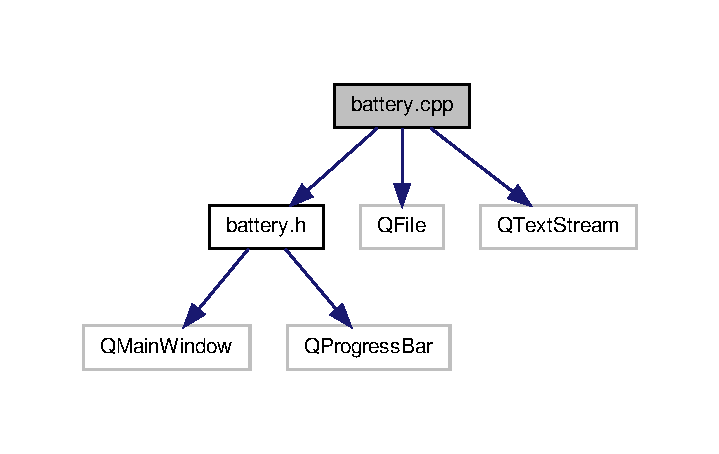
\includegraphics[width=345pt]{battery_8cpp__incl}
\end{center}
\end{figure}


\subsection{Detailed Description}
Ce programme permet l'affichage des états des batteries du drone et du segment sol grâce à des Q\-Progress\-Bar. \begin{DoxyAuthor}{Author}
Martin P\-R\-A\-D\-E\-A\-U / Pierre P\-O\-U\-C\-H 
\end{DoxyAuthor}
\begin{DoxyVersion}{Version}
Version finale 
\end{DoxyVersion}
\begin{DoxyDate}{Date}
Janvier 2014 
\end{DoxyDate}


Definition in file \hyperlink{battery_8cpp_source}{battery.\-cpp}.


\hypertarget{battery_8h}{\section{battery.\-h File Reference}
\label{battery_8h}\index{battery.\-h@{battery.\-h}}
}


Fichier d'inclusion des librairies nécessaires au widget permettant l'affichage de l'état des batteries.  


{\ttfamily \#include $<$Q\-Main\-Window$>$}\\*
{\ttfamily \#include \char`\"{}Q\-Progress\-Bar\char`\"{}}\\*
Include dependency graph for battery.\-h\-:\nopagebreak
\begin{figure}[H]
\begin{center}
\leavevmode
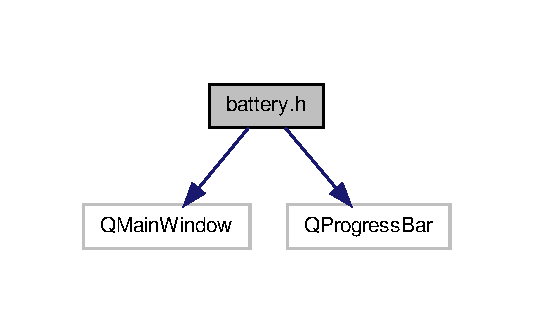
\includegraphics[width=256pt]{battery_8h__incl}
\end{center}
\end{figure}
This graph shows which files directly or indirectly include this file\-:\nopagebreak
\begin{figure}[H]
\begin{center}
\leavevmode
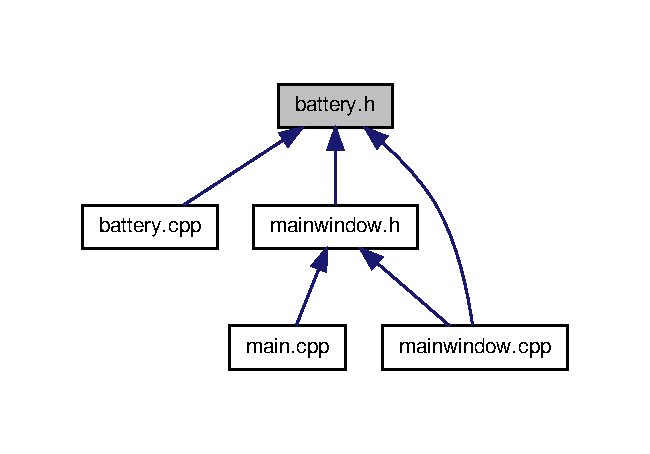
\includegraphics[width=312pt]{battery_8h__dep__incl}
\end{center}
\end{figure}
\subsection*{Classes}
\begin{DoxyCompactItemize}
\item 
class \hyperlink{classbattery}{battery}
\end{DoxyCompactItemize}


\subsection{Detailed Description}
Fichier d'inclusion des librairies nécessaires au widget permettant l'affichage de l'état des batteries. \begin{DoxyAuthor}{Author}
Martin P\-R\-A\-D\-E\-A\-U / Pierre P\-O\-U\-C\-H 
\end{DoxyAuthor}
\begin{DoxyVersion}{Version}
Version finale 
\end{DoxyVersion}
\begin{DoxyDate}{Date}
Janvier 2014 
\end{DoxyDate}


Definition in file \hyperlink{battery_8h_source}{battery.\-h}.


\hypertarget{camerawidget_8cpp}{\section{camerawidget.\-cpp File Reference}
\label{camerawidget_8cpp}\index{camerawidget.\-cpp@{camerawidget.\-cpp}}
}


Ce programme permet la conversion d'une Ipl\-Image en une Q\-Pixmap et le placement du constructeur (widget) dans un layout.  


{\ttfamily \#include \char`\"{}camerawidget.\-h\char`\"{}}\\*
Include dependency graph for camerawidget.\-cpp\-:\nopagebreak
\begin{figure}[H]
\begin{center}
\leavevmode
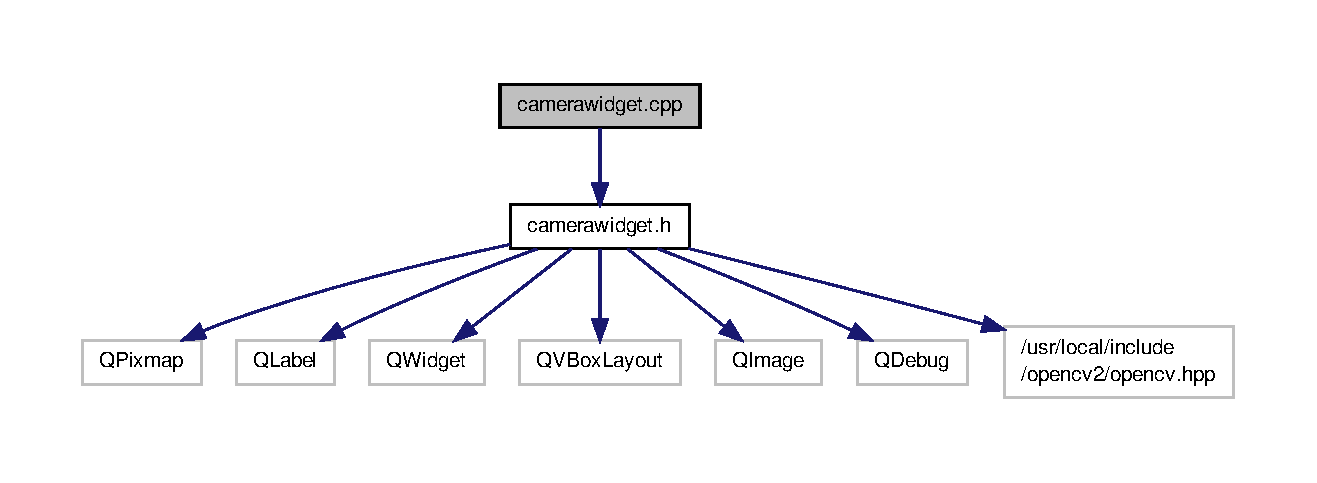
\includegraphics[width=350pt]{camerawidget_8cpp__incl}
\end{center}
\end{figure}


\subsection{Detailed Description}
Ce programme permet la conversion d'une Ipl\-Image en une Q\-Pixmap et le placement du constructeur (widget) dans un layout. \begin{DoxyAuthor}{Author}
Martin P\-R\-A\-D\-E\-A\-U 
\end{DoxyAuthor}
\begin{DoxyVersion}{Version}
Version finale 
\end{DoxyVersion}
\begin{DoxyDate}{Date}
Janvier 2014 
\end{DoxyDate}


Definition in file \hyperlink{camerawidget_8cpp_source}{camerawidget.\-cpp}.


\hypertarget{camerawidget_8h}{\section{camerawidget.\-h File Reference}
\label{camerawidget_8h}\index{camerawidget.\-h@{camerawidget.\-h}}
}


Fichier d'inclusion des librairies nécessaires au widget.  


{\ttfamily \#include $<$Q\-Pixmap$>$}\\*
{\ttfamily \#include $<$Q\-Label$>$}\\*
{\ttfamily \#include $<$Q\-Widget$>$}\\*
{\ttfamily \#include $<$Q\-V\-Box\-Layout$>$}\\*
{\ttfamily \#include $<$Q\-Image$>$}\\*
{\ttfamily \#include $<$Q\-Debug$>$}\\*
{\ttfamily \#include $<$/usr/local/include/opencv2/opencv.\-hpp$>$}\\*
Include dependency graph for camerawidget.\-h\-:\nopagebreak
\begin{figure}[H]
\begin{center}
\leavevmode
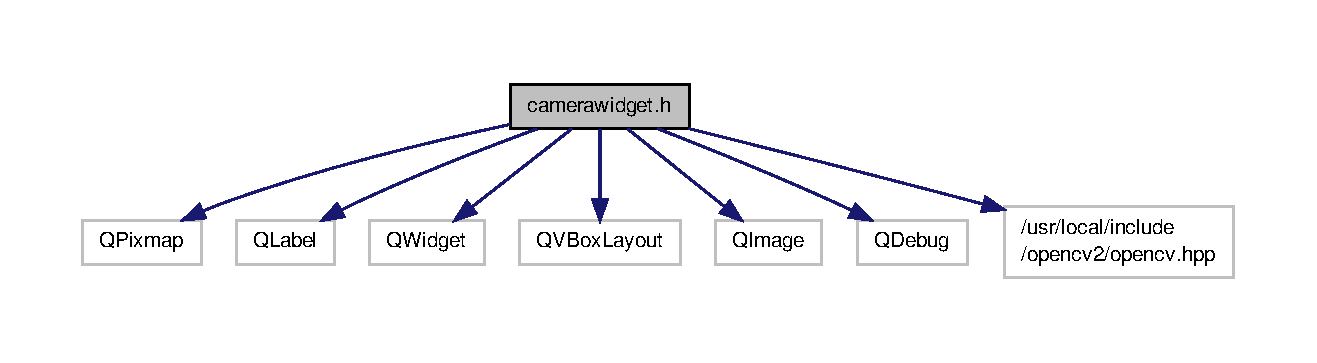
\includegraphics[width=350pt]{camerawidget_8h__incl}
\end{center}
\end{figure}
This graph shows which files directly or indirectly include this file\-:\nopagebreak
\begin{figure}[H]
\begin{center}
\leavevmode
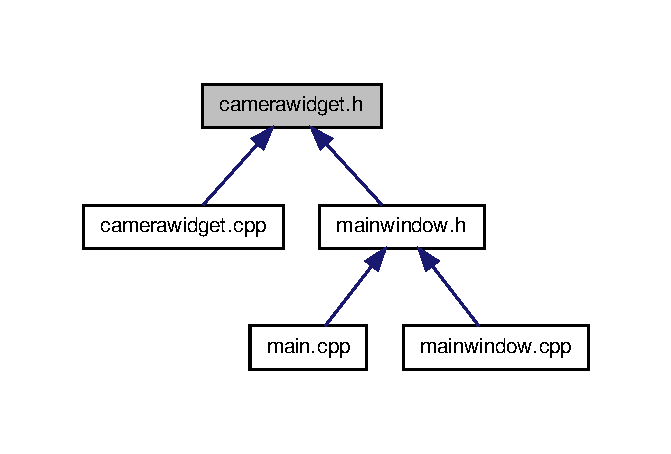
\includegraphics[width=322pt]{camerawidget_8h__dep__incl}
\end{center}
\end{figure}
\subsection*{Classes}
\begin{DoxyCompactItemize}
\item 
class \hyperlink{classCameraWidget}{Camera\-Widget}
\end{DoxyCompactItemize}


\subsection{Detailed Description}
Fichier d'inclusion des librairies nécessaires au widget. \begin{DoxyAuthor}{Author}
Martin P\-R\-A\-D\-E\-A\-U 
\end{DoxyAuthor}
\begin{DoxyVersion}{Version}
Version finale 
\end{DoxyVersion}
\begin{DoxyDate}{Date}
Janvier 2014 
\end{DoxyDate}


Definition in file \hyperlink{camerawidget_8h_source}{camerawidget.\-h}.


\hypertarget{librairie_8h}{\section{librairie.\-h File Reference}
\label{librairie_8h}\index{librairie.\-h@{librairie.\-h}}
}
{\ttfamily \#include $<$stdio.\-h$>$}\\*
{\ttfamily \#include $<$iostream$>$}\\*
{\ttfamily \#include $<$/usr/local/include/opencv2/core/core.\-hpp$>$}\\*
{\ttfamily \#include $<$/usr/local/include/opencv2/features2d/features2d.\-hpp$>$}\\*
{\ttfamily \#include $<$/usr/local/include/opencv2/highgui/highgui.\-hpp$>$}\\*
{\ttfamily \#include $<$/usr/local/include/opencv2/calib3d/calib3d.\-hpp$>$}\\*
{\ttfamily \#include $<$/usr/local/include/opencv2/imgproc/imgproc\-\_\-c.\-h$>$}\\*
{\ttfamily \#include $<$/usr/local/include/opencv2/opencv.\-hpp$>$}\\*
{\ttfamily \#include $<$/usr/local/include/opencv2/contrib/contrib.\-hpp$>$}\\*
{\ttfamily \#include $<$/usr/local/include/opencv2/objdetect/objdetect.\-hpp$>$}\\*
{\ttfamily \#include $<$thread$>$}\\*
{\ttfamily \#include $<$vector$>$}\\*
Include dependency graph for librairie.\-h\-:\nopagebreak
\begin{figure}[H]
\begin{center}
\leavevmode
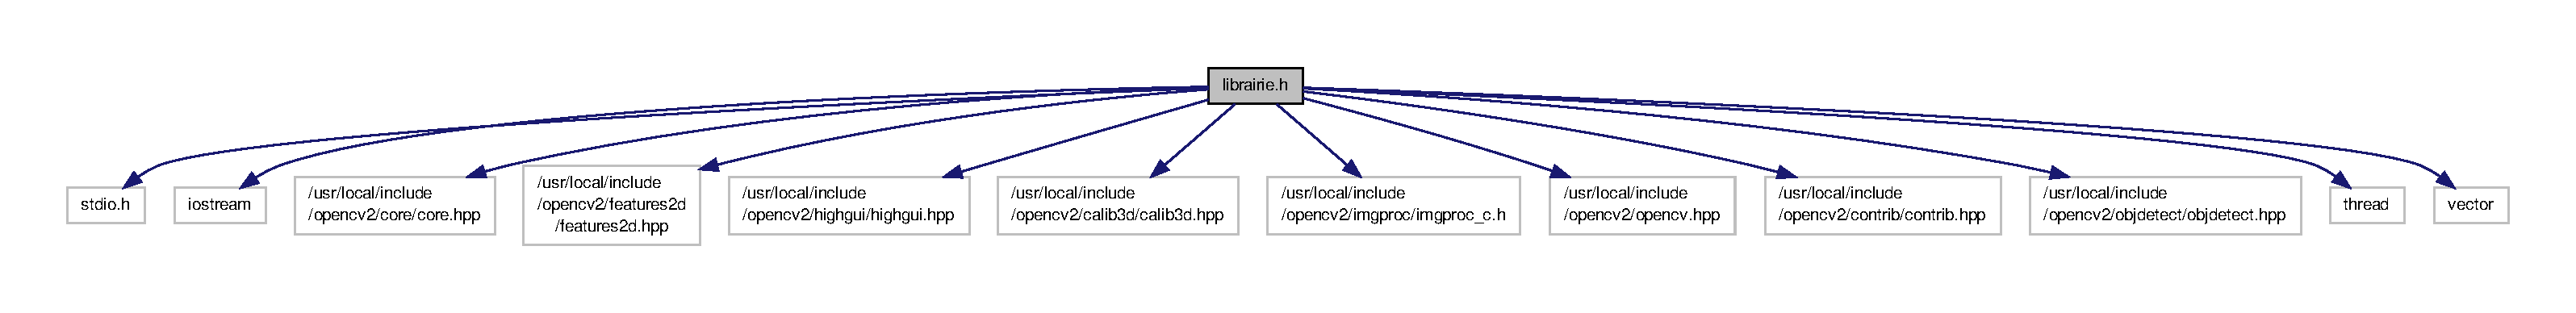
\includegraphics[width=350pt]{librairie_8h__incl}
\end{center}
\end{figure}
This graph shows which files directly or indirectly include this file\-:\nopagebreak
\begin{figure}[H]
\begin{center}
\leavevmode
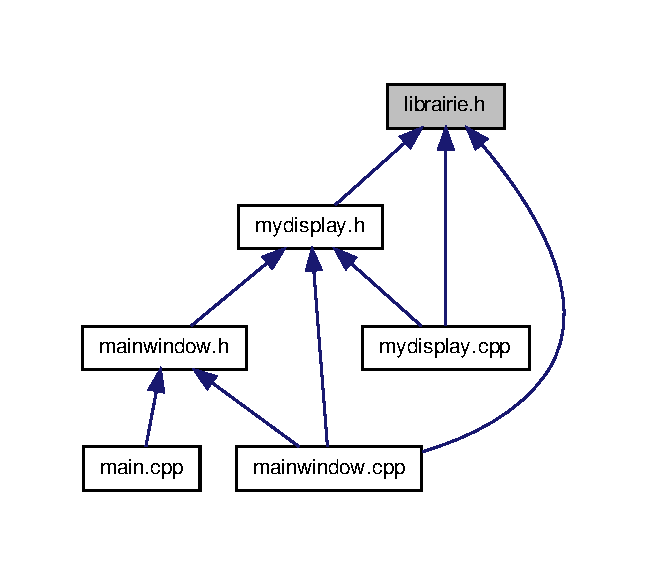
\includegraphics[width=311pt]{librairie_8h__dep__incl}
\end{center}
\end{figure}
\subsection*{Macros}
\begin{DoxyCompactItemize}
\item 
\#define \hyperlink{librairie_8h_a8777987cdbdc1570c0a5fa97c7366847}{L\-U\-B\-R\-A\-I\-R\-I\-E\-\_\-\-H}
\end{DoxyCompactItemize}


\subsection{Macro Definition Documentation}
\hypertarget{librairie_8h_a8777987cdbdc1570c0a5fa97c7366847}{\index{librairie.\-h@{librairie.\-h}!L\-U\-B\-R\-A\-I\-R\-I\-E\-\_\-\-H@{L\-U\-B\-R\-A\-I\-R\-I\-E\-\_\-\-H}}
\index{L\-U\-B\-R\-A\-I\-R\-I\-E\-\_\-\-H@{L\-U\-B\-R\-A\-I\-R\-I\-E\-\_\-\-H}!librairie.h@{librairie.\-h}}
\subsubsection[{L\-U\-B\-R\-A\-I\-R\-I\-E\-\_\-\-H}]{\setlength{\rightskip}{0pt plus 5cm}\#define L\-U\-B\-R\-A\-I\-R\-I\-E\-\_\-\-H}}\label{librairie_8h_a8777987cdbdc1570c0a5fa97c7366847}


Definition at line 2 of file librairie.\-h.


\hypertarget{lightmaps_8cpp}{\section{lightmaps.\-cpp File Reference}
\label{lightmaps_8cpp}\index{lightmaps.\-cpp@{lightmaps.\-cpp}}
}
{\ttfamily \#include $<$Qt\-Core$>$}\\*
{\ttfamily \#include $<$Qt\-Gui$>$}\\*
{\ttfamily \#include $<$Qt\-Network$>$}\\*
{\ttfamily \#include $<$math.\-h$>$}\\*
{\ttfamily \#include \char`\"{}lightmaps.\-h\char`\"{}}\\*
{\ttfamily \#include \char`\"{}slippymap.\-h\char`\"{}}\\*
Include dependency graph for lightmaps.\-cpp\-:\nopagebreak
\begin{figure}[H]
\begin{center}
\leavevmode
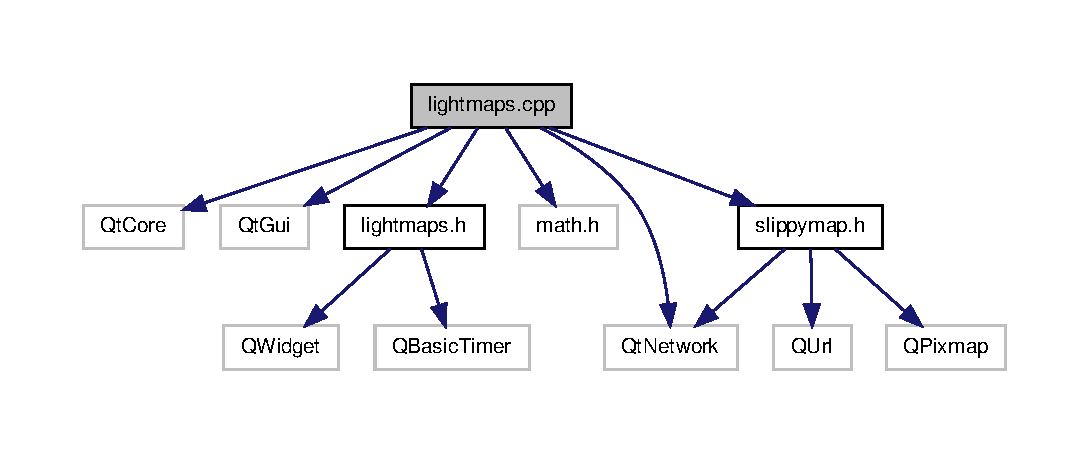
\includegraphics[width=350pt]{lightmaps_8cpp__incl}
\end{center}
\end{figure}
\subsection*{Macros}
\begin{DoxyCompactItemize}
\item 
\#define \hyperlink{lightmaps_8cpp_ae71449b1cc6e6250b91f539153a7a0d3}{M\-\_\-\-P\-I}~3.\-14159265358979323846
\item 
\#define \hyperlink{lightmaps_8cpp_a3f171629948a6f7ad5c9e9a4d9f1366c}{H\-O\-L\-D\-\_\-\-T\-I\-M\-E}~701
\item 
\#define \hyperlink{lightmaps_8cpp_a51ac6ea721e00a4f2396493f9517b9e5}{M\-A\-X\-\_\-\-M\-A\-G\-N\-I\-F\-I\-E\-R}~229
\end{DoxyCompactItemize}


\subsection{Macro Definition Documentation}
\hypertarget{lightmaps_8cpp_a3f171629948a6f7ad5c9e9a4d9f1366c}{\index{lightmaps.\-cpp@{lightmaps.\-cpp}!H\-O\-L\-D\-\_\-\-T\-I\-M\-E@{H\-O\-L\-D\-\_\-\-T\-I\-M\-E}}
\index{H\-O\-L\-D\-\_\-\-T\-I\-M\-E@{H\-O\-L\-D\-\_\-\-T\-I\-M\-E}!lightmaps.cpp@{lightmaps.\-cpp}}
\subsubsection[{H\-O\-L\-D\-\_\-\-T\-I\-M\-E}]{\setlength{\rightskip}{0pt plus 5cm}\#define H\-O\-L\-D\-\_\-\-T\-I\-M\-E~701}}\label{lightmaps_8cpp_a3f171629948a6f7ad5c9e9a4d9f1366c}


Definition at line 16 of file lightmaps.\-cpp.



Referenced by Light\-Maps\-::mouse\-Press\-Event().

\hypertarget{lightmaps_8cpp_ae71449b1cc6e6250b91f539153a7a0d3}{\index{lightmaps.\-cpp@{lightmaps.\-cpp}!M\-\_\-\-P\-I@{M\-\_\-\-P\-I}}
\index{M\-\_\-\-P\-I@{M\-\_\-\-P\-I}!lightmaps.cpp@{lightmaps.\-cpp}}
\subsubsection[{M\-\_\-\-P\-I}]{\setlength{\rightskip}{0pt plus 5cm}\#define M\-\_\-\-P\-I~3.\-14159265358979323846}}\label{lightmaps_8cpp_ae71449b1cc6e6250b91f539153a7a0d3}


Definition at line 9 of file lightmaps.\-cpp.

\hypertarget{lightmaps_8cpp_a51ac6ea721e00a4f2396493f9517b9e5}{\index{lightmaps.\-cpp@{lightmaps.\-cpp}!M\-A\-X\-\_\-\-M\-A\-G\-N\-I\-F\-I\-E\-R@{M\-A\-X\-\_\-\-M\-A\-G\-N\-I\-F\-I\-E\-R}}
\index{M\-A\-X\-\_\-\-M\-A\-G\-N\-I\-F\-I\-E\-R@{M\-A\-X\-\_\-\-M\-A\-G\-N\-I\-F\-I\-E\-R}!lightmaps.cpp@{lightmaps.\-cpp}}
\subsubsection[{M\-A\-X\-\_\-\-M\-A\-G\-N\-I\-F\-I\-E\-R}]{\setlength{\rightskip}{0pt plus 5cm}\#define M\-A\-X\-\_\-\-M\-A\-G\-N\-I\-F\-I\-E\-R~229}}\label{lightmaps_8cpp_a51ac6ea721e00a4f2396493f9517b9e5}


Definition at line 20 of file lightmaps.\-cpp.



Referenced by Light\-Maps\-::paint\-Event().


\hypertarget{lightmaps_8h}{\section{lightmaps.\-h File Reference}
\label{lightmaps_8h}\index{lightmaps.\-h@{lightmaps.\-h}}
}
{\ttfamily \#include $<$Q\-Basic\-Timer$>$}\\*
{\ttfamily \#include $<$Q\-Widget$>$}\\*
Include dependency graph for lightmaps.\-h\-:\nopagebreak
\begin{figure}[H]
\begin{center}
\leavevmode
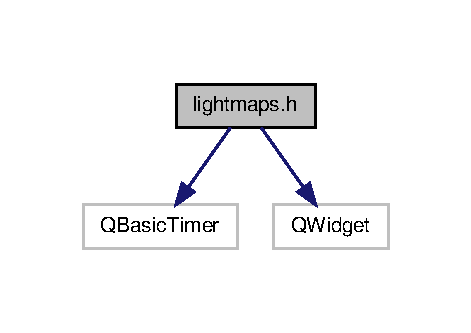
\includegraphics[width=226pt]{lightmaps_8h__incl}
\end{center}
\end{figure}
This graph shows which files directly or indirectly include this file\-:\nopagebreak
\begin{figure}[H]
\begin{center}
\leavevmode
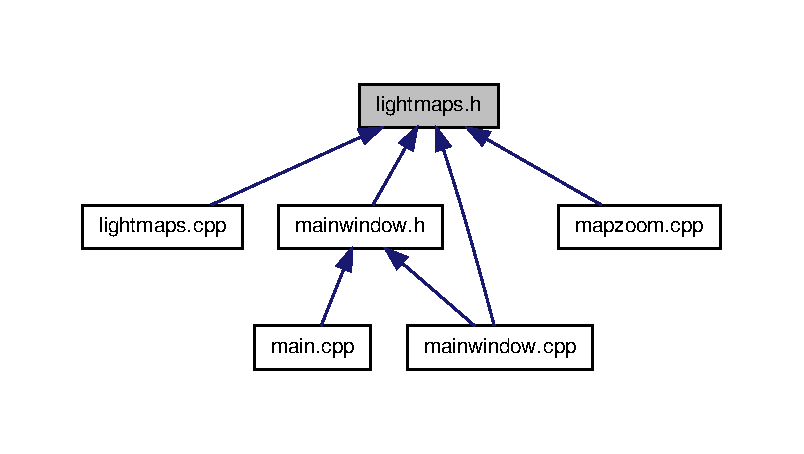
\includegraphics[width=350pt]{lightmaps_8h__dep__incl}
\end{center}
\end{figure}
\subsection*{Classes}
\begin{DoxyCompactItemize}
\item 
class \hyperlink{classLightMaps}{Light\-Maps}
\end{DoxyCompactItemize}

\hypertarget{main_8cpp}{\section{main.\-cpp File Reference}
\label{main_8cpp}\index{main.\-cpp@{main.\-cpp}}
}


Ficher main qui permet d'afficher la \hyperlink{classMainWindow}{Main\-Window}.  


{\ttfamily \#include $<$Q\-Application$>$}\\*
{\ttfamily \#include \char`\"{}mainwindow.\-h\char`\"{}}\\*
Include dependency graph for main.\-cpp\-:\nopagebreak
\begin{figure}[H]
\begin{center}
\leavevmode
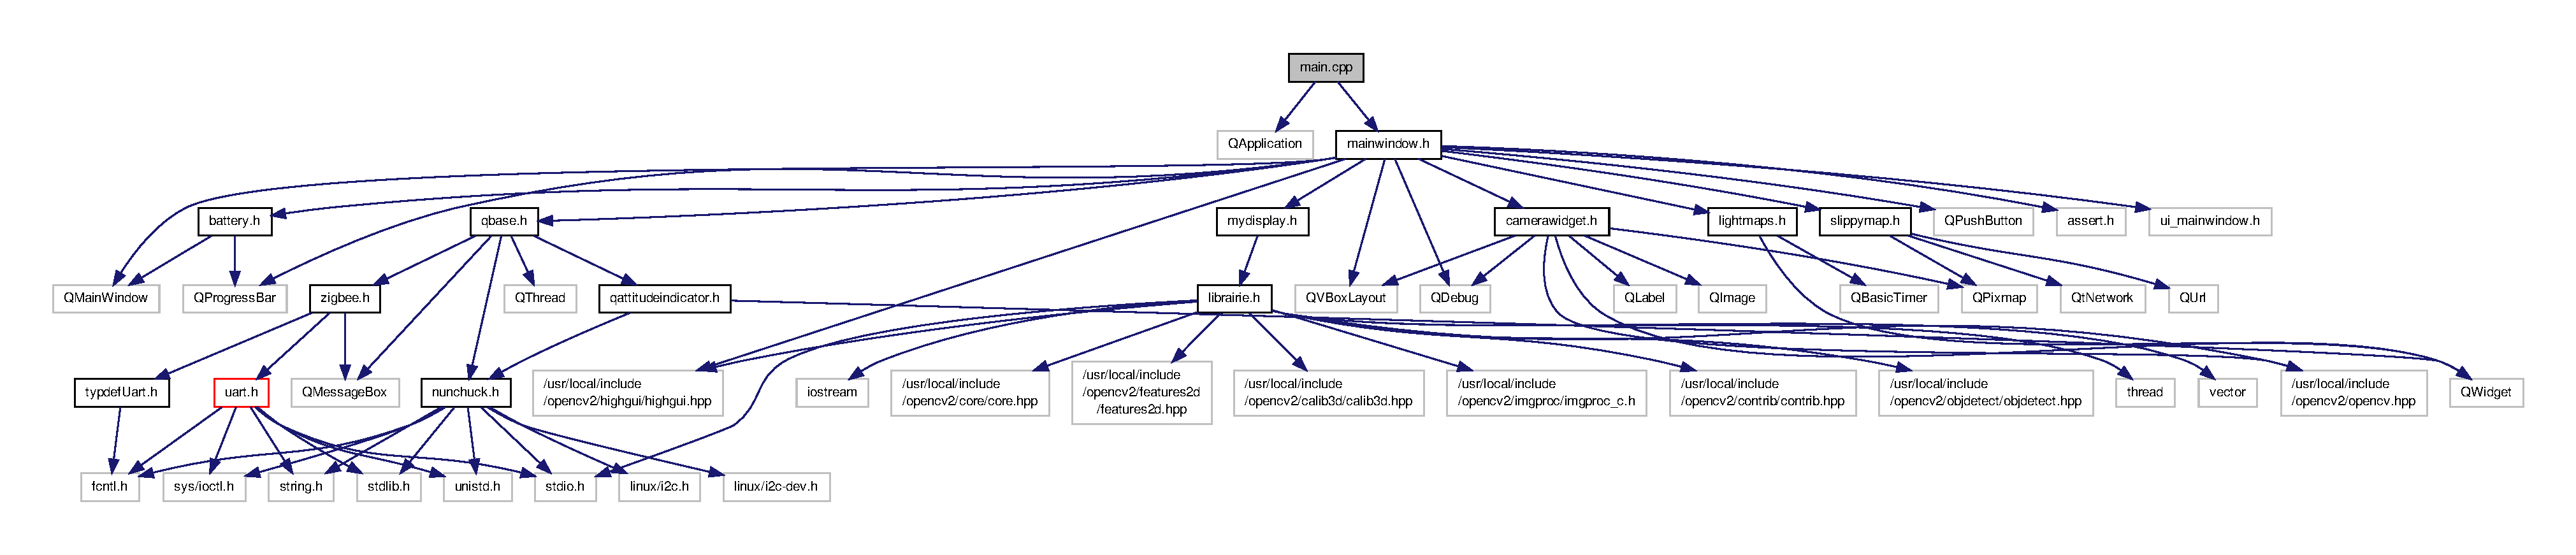
\includegraphics[width=350pt]{main_8cpp__incl}
\end{center}
\end{figure}
\subsection*{Functions}
\begin{DoxyCompactItemize}
\item 
int \hyperlink{main_8cpp_a3c04138a5bfe5d72780bb7e82a18e627}{main} (int argc, char $\ast$$\ast$argv)
\end{DoxyCompactItemize}


\subsection{Detailed Description}
Ficher main qui permet d'afficher la \hyperlink{classMainWindow}{Main\-Window}. \begin{DoxyAuthor}{Author}
Martin P\-R\-A\-D\-E\-A\-U 
\end{DoxyAuthor}
\begin{DoxyVersion}{Version}
Version finale 
\end{DoxyVersion}
\begin{DoxyDate}{Date}
Janvier 2014 
\end{DoxyDate}


Definition in file \hyperlink{main_8cpp_source}{main.\-cpp}.



\subsection{Function Documentation}
\hypertarget{main_8cpp_a3c04138a5bfe5d72780bb7e82a18e627}{\index{main.\-cpp@{main.\-cpp}!main@{main}}
\index{main@{main}!main.cpp@{main.\-cpp}}
\subsubsection[{main}]{\setlength{\rightskip}{0pt plus 5cm}int main (
\begin{DoxyParamCaption}
\item[{int}]{argc, }
\item[{char $\ast$$\ast$}]{argv}
\end{DoxyParamCaption}
)}}\label{main_8cpp_a3c04138a5bfe5d72780bb7e82a18e627}


Definition at line 58 of file main.\-cpp.


\begin{DoxyCode}
\{

    QApplication app(argc, argv);
    \hyperlink{classMainWindow}{MainWindow} w;
    w.show();

    \textcolor{keywordtype}{int} retval = app.exec();
    \textcolor{keywordflow}{return} retval;
\}
\end{DoxyCode}

\hypertarget{mainwindow_8cpp}{\section{mainwindow.\-cpp File Reference}
\label{mainwindow_8cpp}\index{mainwindow.\-cpp@{mainwindow.\-cpp}}
}


Ce programme permet le placement de tous les widgets ou objets nécessaires au fonctionnement de l'application.  


{\ttfamily \#include $<$Qt\-Gui/\-Q\-Application$>$}\\*
{\ttfamily \#include \char`\"{}mainwindow.\-h\char`\"{}}\\*
{\ttfamily \#include \char`\"{}librairie.\-h\char`\"{}}\\*
{\ttfamily \#include \char`\"{}mydisplay.\-h\char`\"{}}\\*
{\ttfamily \#include \char`\"{}battery.\-h\char`\"{}}\\*
{\ttfamily \#include $<$Qt\-Gui$>$}\\*
{\ttfamily \#include $<$Qt\-Network$>$}\\*
{\ttfamily \#include $<$Q\-Text\-Stream$>$}\\*
{\ttfamily \#include $<$Q\-String$>$}\\*
{\ttfamily \#include $<$Q\-File$>$}\\*
{\ttfamily \#include $<$Q\-I\-O\-Device$>$}\\*
{\ttfamily \#include $<$Q\-Vector$>$}\\*
{\ttfamily \#include $<$Q\-Painter$>$}\\*
{\ttfamily \#include \char`\"{}lightmaps.\-h\char`\"{}}\\*
{\ttfamily \#include \char`\"{}slippymap.\-h\char`\"{}}\\*
{\ttfamily \#include $<$stdio.\-h$>$}\\*
{\ttfamily \#include $<$stdlib.\-h$>$}\\*
{\ttfamily \#include $<$fstream$>$}\\*
{\ttfamily \#include $<$Qt\-Gui/qgridlayout.\-h$>$}\\*
Include dependency graph for mainwindow.\-cpp\-:\nopagebreak
\begin{figure}[H]
\begin{center}
\leavevmode
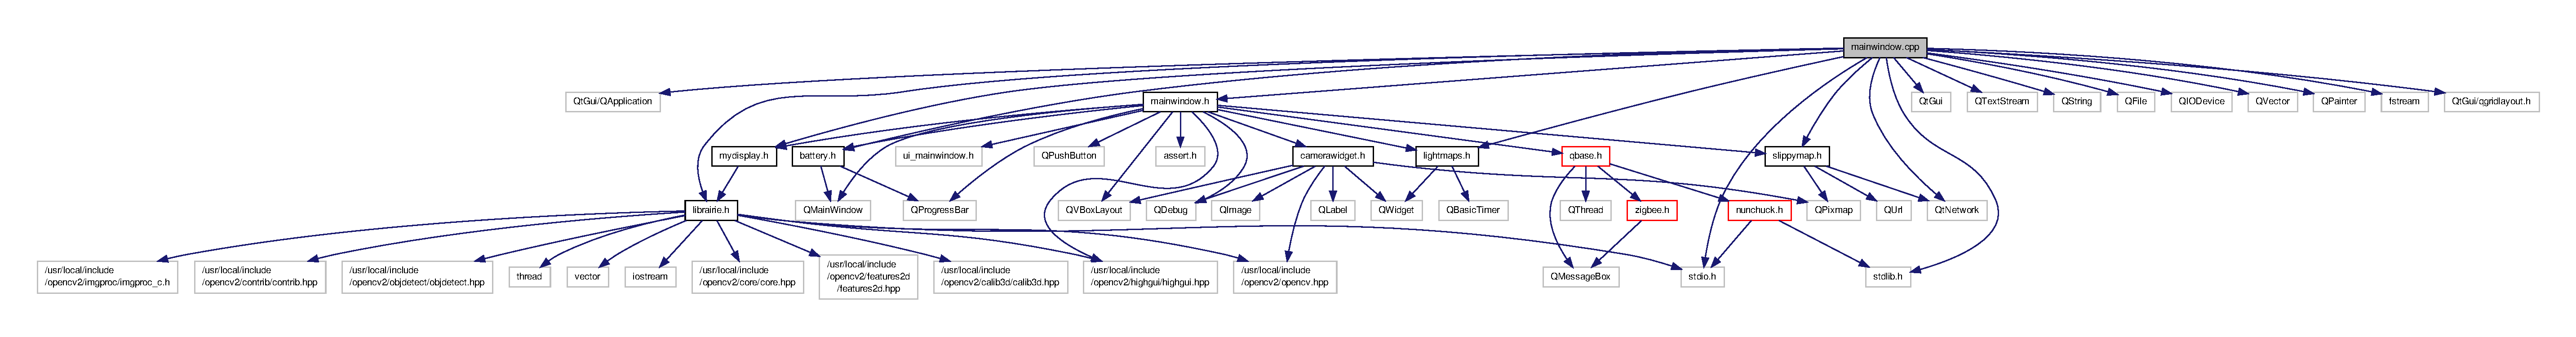
\includegraphics[width=350pt]{mainwindow_8cpp__incl}
\end{center}
\end{figure}


\subsection{Detailed Description}
Ce programme permet le placement de tous les widgets ou objets nécessaires au fonctionnement de l'application. \begin{DoxyAuthor}{Author}
Martin P\-R\-A\-D\-E\-A\-U 
\end{DoxyAuthor}
\begin{DoxyVersion}{Version}
Version finale 
\end{DoxyVersion}
\begin{DoxyDate}{Date}
Janvier 2014 
\end{DoxyDate}


Definition in file \hyperlink{mainwindow_8cpp_source}{mainwindow.\-cpp}.


\hypertarget{mainwindow_8h}{\section{mainwindow.\-h File Reference}
\label{mainwindow_8h}\index{mainwindow.\-h@{mainwindow.\-h}}
}


Fichier d'inclusion des librairies nécessaires à la \hyperlink{classMainWindow}{Main\-Window}.  


{\ttfamily \#include $<$Q\-Main\-Window$>$}\\*
{\ttfamily \#include $<$Q\-V\-Box\-Layout$>$}\\*
{\ttfamily \#include $<$Q\-Debug$>$}\\*
{\ttfamily \#include $<$Q\-Push\-Button$>$}\\*
{\ttfamily \#include $<$/usr/local/include/opencv2/highgui/highgui.\-hpp$>$}\\*
{\ttfamily \#include $<$assert.\-h$>$}\\*
{\ttfamily \#include \char`\"{}mydisplay.\-h\char`\"{}}\\*
{\ttfamily \#include \char`\"{}camerawidget.\-h\char`\"{}}\\*
{\ttfamily \#include \char`\"{}qbase.\-h\char`\"{}}\\*
{\ttfamily \#include \char`\"{}battery.\-h\char`\"{}}\\*
{\ttfamily \#include \char`\"{}ui\-\_\-mainwindow.\-h\char`\"{}}\\*
{\ttfamily \#include \char`\"{}lightmaps.\-h\char`\"{}}\\*
{\ttfamily \#include \char`\"{}slippymap.\-h\char`\"{}}\\*
{\ttfamily \#include \char`\"{}Q\-Progress\-Bar\char`\"{}}\\*
Include dependency graph for mainwindow.\-h\-:\nopagebreak
\begin{figure}[H]
\begin{center}
\leavevmode
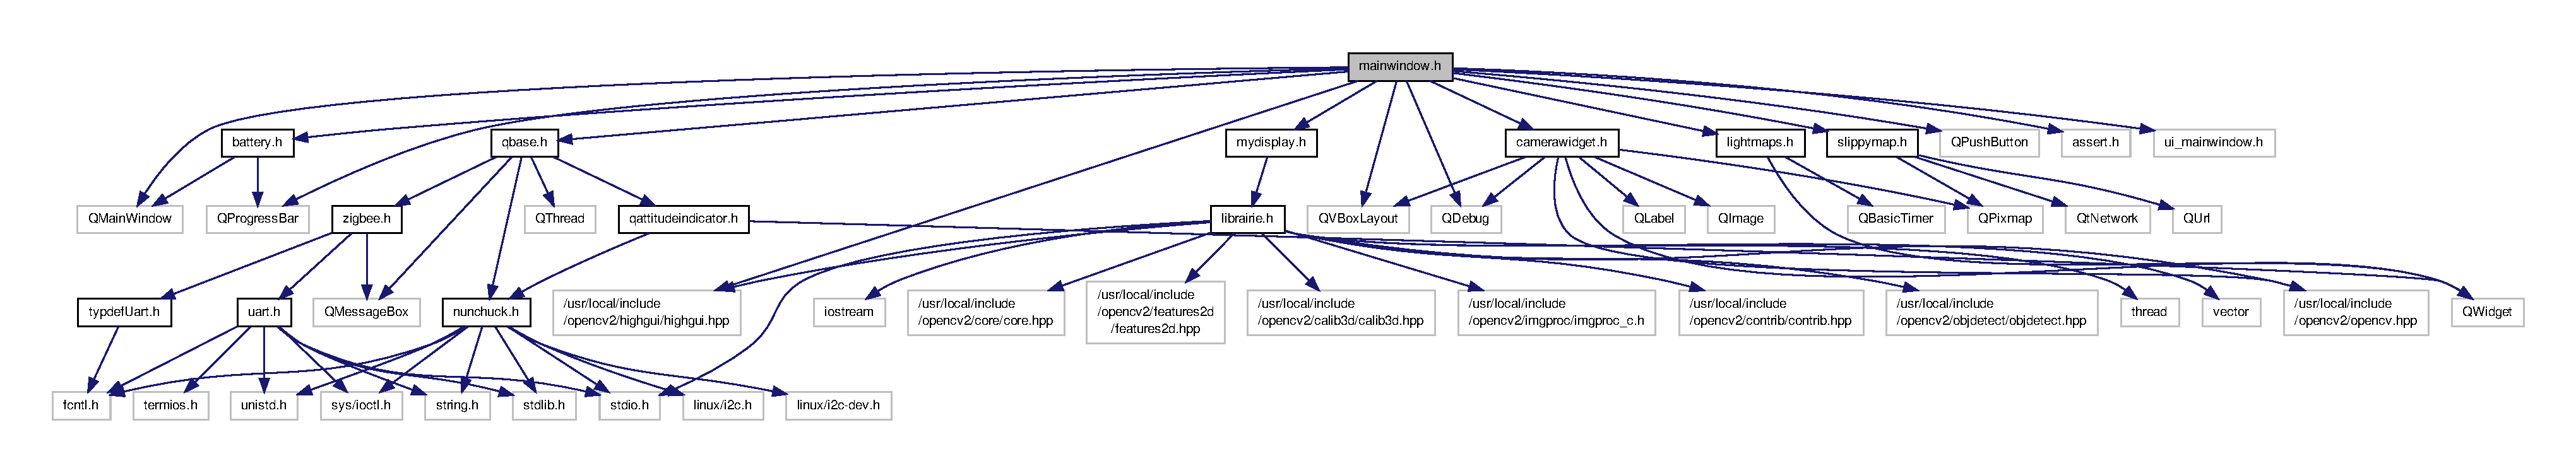
\includegraphics[width=350pt]{mainwindow_8h__incl}
\end{center}
\end{figure}
This graph shows which files directly or indirectly include this file\-:\nopagebreak
\begin{figure}[H]
\begin{center}
\leavevmode
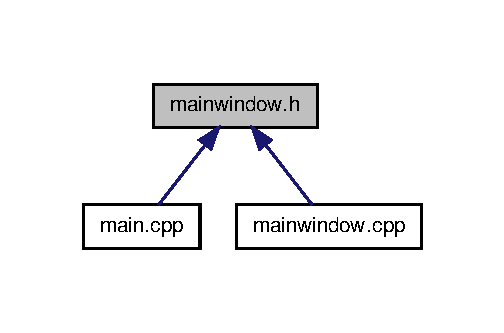
\includegraphics[width=242pt]{mainwindow_8h__dep__incl}
\end{center}
\end{figure}
\subsection*{Classes}
\begin{DoxyCompactItemize}
\item 
class \hyperlink{classMainWindow}{Main\-Window}
\end{DoxyCompactItemize}
\subsection*{Namespaces}
\begin{DoxyCompactItemize}
\item 
namespace \hyperlink{namespaceUi}{Ui}
\end{DoxyCompactItemize}
\subsection*{Macros}
\begin{DoxyCompactItemize}
\item 
\#define \hyperlink{mainwindow_8h_ab9f3d4f131379475d4b36a15d2b59b5e}{I\-N\-D\-E\-X\-\_\-\-O\-N\-G\-L\-E\-T\-\_\-\-C\-A\-M\-E\-R\-A}~0
\item 
\#define \hyperlink{mainwindow_8h_ac416243e121530c2fc222e5204d7fe30}{I\-N\-D\-E\-X\-\_\-\-O\-N\-G\-L\-E\-T\-\_\-\-H\-O\-R\-I\-Z\-O\-N}~1
\end{DoxyCompactItemize}


\subsection{Detailed Description}
Fichier d'inclusion des librairies nécessaires à la \hyperlink{classMainWindow}{Main\-Window}. \begin{DoxyAuthor}{Author}
Martin P\-R\-A\-D\-E\-A\-U 
\end{DoxyAuthor}
\begin{DoxyVersion}{Version}
Version finale 
\end{DoxyVersion}
\begin{DoxyDate}{Date}
Janvier 2014 
\end{DoxyDate}


Definition in file \hyperlink{mainwindow_8h_source}{mainwindow.\-h}.



\subsection{Macro Definition Documentation}
\hypertarget{mainwindow_8h_ab9f3d4f131379475d4b36a15d2b59b5e}{\index{mainwindow.\-h@{mainwindow.\-h}!I\-N\-D\-E\-X\-\_\-\-O\-N\-G\-L\-E\-T\-\_\-\-C\-A\-M\-E\-R\-A@{I\-N\-D\-E\-X\-\_\-\-O\-N\-G\-L\-E\-T\-\_\-\-C\-A\-M\-E\-R\-A}}
\index{I\-N\-D\-E\-X\-\_\-\-O\-N\-G\-L\-E\-T\-\_\-\-C\-A\-M\-E\-R\-A@{I\-N\-D\-E\-X\-\_\-\-O\-N\-G\-L\-E\-T\-\_\-\-C\-A\-M\-E\-R\-A}!mainwindow.h@{mainwindow.\-h}}
\subsubsection[{I\-N\-D\-E\-X\-\_\-\-O\-N\-G\-L\-E\-T\-\_\-\-C\-A\-M\-E\-R\-A}]{\setlength{\rightskip}{0pt plus 5cm}\#define I\-N\-D\-E\-X\-\_\-\-O\-N\-G\-L\-E\-T\-\_\-\-C\-A\-M\-E\-R\-A~0}}\label{mainwindow_8h_ab9f3d4f131379475d4b36a15d2b59b5e}


Definition at line 29 of file mainwindow.\-h.



Referenced by Main\-Window\-::\-Change\-Onglet(), and Main\-Window\-::timer\-Event().

\hypertarget{mainwindow_8h_ac416243e121530c2fc222e5204d7fe30}{\index{mainwindow.\-h@{mainwindow.\-h}!I\-N\-D\-E\-X\-\_\-\-O\-N\-G\-L\-E\-T\-\_\-\-H\-O\-R\-I\-Z\-O\-N@{I\-N\-D\-E\-X\-\_\-\-O\-N\-G\-L\-E\-T\-\_\-\-H\-O\-R\-I\-Z\-O\-N}}
\index{I\-N\-D\-E\-X\-\_\-\-O\-N\-G\-L\-E\-T\-\_\-\-H\-O\-R\-I\-Z\-O\-N@{I\-N\-D\-E\-X\-\_\-\-O\-N\-G\-L\-E\-T\-\_\-\-H\-O\-R\-I\-Z\-O\-N}!mainwindow.h@{mainwindow.\-h}}
\subsubsection[{I\-N\-D\-E\-X\-\_\-\-O\-N\-G\-L\-E\-T\-\_\-\-H\-O\-R\-I\-Z\-O\-N}]{\setlength{\rightskip}{0pt plus 5cm}\#define I\-N\-D\-E\-X\-\_\-\-O\-N\-G\-L\-E\-T\-\_\-\-H\-O\-R\-I\-Z\-O\-N~1}}\label{mainwindow_8h_ac416243e121530c2fc222e5204d7fe30}


Definition at line 30 of file mainwindow.\-h.



Referenced by Main\-Window\-::\-Change\-Onglet().


\hypertarget{mainwindow_8ui}{\section{mainwindow.\-ui File Reference}
\label{mainwindow_8ui}\index{mainwindow.\-ui@{mainwindow.\-ui}}
}
\subsection*{Variables}
\begin{DoxyCompactItemize}
\item 
$<$?xmlversion=\char`\"{}1.\-0\char`\"{}encoding=\char`\"{}U\-T\-F-\/8\char`\"{}?$>$\\*
$<$ uiversion=\char`\"{}4.\-0\char`\"{}$>$$<$ class $>$\\*
 \hyperlink{classMainWindow}{Main\-Window}$<$/class $>$\\*
$<$ widgetclass=\char`\"{}Q\-Main\-Window\char`\"{}name=\char`\"{}Main\-Window\char`\"{}$>$\\*
$<$ propertyname=\char`\"{}enabled\char`\"{}$>$\\*
$<$ bool $>$ true$<$/bool $>$\\*
$<$/property $>$$<$ propertyname=\char`\"{}geometry\char`\"{}$>$\\*
$<$ rect $>$$<$ x $>$$<$/x $>$$<$ y $>$$<$/y $>$\\*
$<$ width $>$$<$/width $>$$<$ height $>$\\*
$<$/height $>$$<$/rect $>$$<$/property $>$\\*
$<$ propertyname=\char`\"{}minimum\-Size\char`\"{}$>$\\*
$<$ size $>$$<$ width $>$$<$/width $>$\\*
$<$ height $>$$<$/height $>$$<$/size $>$\\*
$<$/property $>$$<$ propertyname=\char`\"{}window\-Title\char`\"{}$>$\\*
$<$ string $>$ \hyperlink{classMainWindow}{Main\-Window}$<$/string $>$\\*
$<$/property $>$$<$ widgetclass=\char`\"{}Q\-Widget\char`\"{}name=\char`\"{}widget\-\_\-principal\char`\"{}$>$\\*
$<$ widgetclass=\char`\"{}Q\-Tab\-Widget\char`\"{}name=\char`\"{}Onglet\char`\"{}$>$\\*
$<$ propertyname=\char`\"{}geometry\char`\"{}$>$\\*
$<$ rect $>$$<$ x $>$$<$/x $>$$<$ y $>$$<$/y $>$\\*
$<$ width $>$$<$/width $>$$<$ height $>$\\*
$<$/height $>$$<$/rect $>$$<$/property $>$\\*
$<$ propertyname=\char`\"{}whats\-This\char`\"{}$>$\\*
$<$ string $>$ \& \hyperlink{mainwindow_8ui_a857c8c8ca640fb2283d751a715bd1ee9}{lt}
\item 
html \& \hyperlink{mainwindow_8ui_acc2b3ab3dd842d17613f7a6cbf7f275d}{gt}
\item 
p \hyperlink{mainwindow_8ui_ab28bdaf6ad2b6aba883d92e474f75867}{align} = \&\hyperlink{mainwindow_8ui_a6ac641f7a2ac50c1fa0b167e88309133}{quot}
\item 
right \& \hyperlink{mainwindow_8ui_a6ac641f7a2ac50c1fa0b167e88309133}{quot}
\end{DoxyCompactItemize}


\subsection{Variable Documentation}
\hypertarget{mainwindow_8ui_ab28bdaf6ad2b6aba883d92e474f75867}{\index{mainwindow.\-ui@{mainwindow.\-ui}!align@{align}}
\index{align@{align}!mainwindow.ui@{mainwindow.\-ui}}
\subsubsection[{align}]{\setlength{\rightskip}{0pt plus 5cm}p align = \&{\bf quot}}}\label{mainwindow_8ui_ab28bdaf6ad2b6aba883d92e474f75867}


Definition at line 36 of file mainwindow.\-ui.

\hypertarget{mainwindow_8ui_acc2b3ab3dd842d17613f7a6cbf7f275d}{\index{mainwindow.\-ui@{mainwindow.\-ui}!gt@{gt}}
\index{gt@{gt}!mainwindow.ui@{mainwindow.\-ui}}
\subsubsection[{gt}]{\setlength{\rightskip}{0pt plus 5cm}html \& gt}}\label{mainwindow_8ui_acc2b3ab3dd842d17613f7a6cbf7f275d}


Definition at line 36 of file mainwindow.\-ui.

\hypertarget{mainwindow_8ui_a857c8c8ca640fb2283d751a715bd1ee9}{\index{mainwindow.\-ui@{mainwindow.\-ui}!lt@{lt}}
\index{lt@{lt}!mainwindow.ui@{mainwindow.\-ui}}
\subsubsection[{lt}]{\setlength{\rightskip}{0pt plus 5cm}\& lt}}\label{mainwindow_8ui_a857c8c8ca640fb2283d751a715bd1ee9}


Definition at line 36 of file mainwindow.\-ui.

\hypertarget{mainwindow_8ui_a6ac641f7a2ac50c1fa0b167e88309133}{\index{mainwindow.\-ui@{mainwindow.\-ui}!quot@{quot}}
\index{quot@{quot}!mainwindow.ui@{mainwindow.\-ui}}
\subsubsection[{quot}]{\setlength{\rightskip}{0pt plus 5cm}right\& quot}}\label{mainwindow_8ui_a6ac641f7a2ac50c1fa0b167e88309133}


Definition at line 36 of file mainwindow.\-ui.


\hypertarget{mapzoom_8cpp}{\section{mapzoom.\-cpp File Reference}
\label{mapzoom_8cpp}\index{mapzoom.\-cpp@{mapzoom.\-cpp}}
}
{\ttfamily \#include $<$Qt\-Gui$>$}\\*
{\ttfamily \#include $<$Qt\-Network$>$}\\*
{\ttfamily \#include $<$Q\-Text\-Stream$>$}\\*
{\ttfamily \#include $<$Q\-String$>$}\\*
{\ttfamily \#include $<$Q\-File$>$}\\*
{\ttfamily \#include $<$Q\-I\-O\-Device$>$}\\*
{\ttfamily \#include $<$Q\-Vector$>$}\\*
{\ttfamily \#include $<$Q\-Painter$>$}\\*
{\ttfamily \#include \char`\"{}lightmaps.\-h\char`\"{}}\\*
{\ttfamily \#include \char`\"{}mapzoom.\-h\char`\"{}}\\*
{\ttfamily \#include \char`\"{}slippymap.\-h\char`\"{}}\\*
{\ttfamily \#include $<$stdio.\-h$>$}\\*
{\ttfamily \#include $<$stdlib.\-h$>$}\\*
Include dependency graph for mapzoom.\-cpp\-:\nopagebreak
\begin{figure}[H]
\begin{center}
\leavevmode
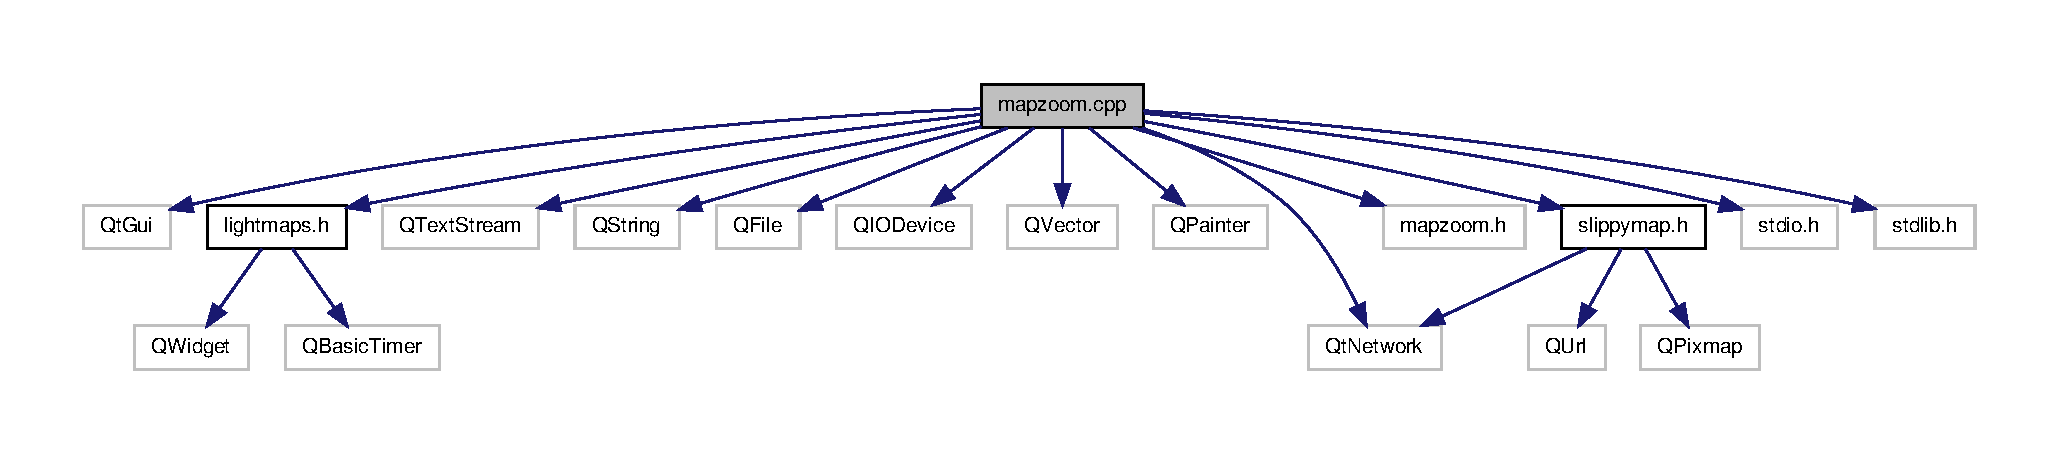
\includegraphics[width=350pt]{mapzoom_8cpp__incl}
\end{center}
\end{figure}

\hypertarget{mydisplay_8cpp}{\section{mydisplay.\-cpp File Reference}
\label{mydisplay_8cpp}\index{mydisplay.\-cpp@{mydisplay.\-cpp}}
}
{\ttfamily \#include \char`\"{}mydisplay.\-h\char`\"{}}\\*
{\ttfamily \#include \char`\"{}librairie.\-h\char`\"{}}\\*
{\ttfamily \#include $<$/usr/local/include/opencv/cv.\-h$>$}\\*
{\ttfamily \#include $<$/usr/local/include/opencv/highgui.\-h$>$}\\*
{\ttfamily \#include $<$assert.\-h$>$}\\*
Include dependency graph for mydisplay.\-cpp\-:\nopagebreak
\begin{figure}[H]
\begin{center}
\leavevmode
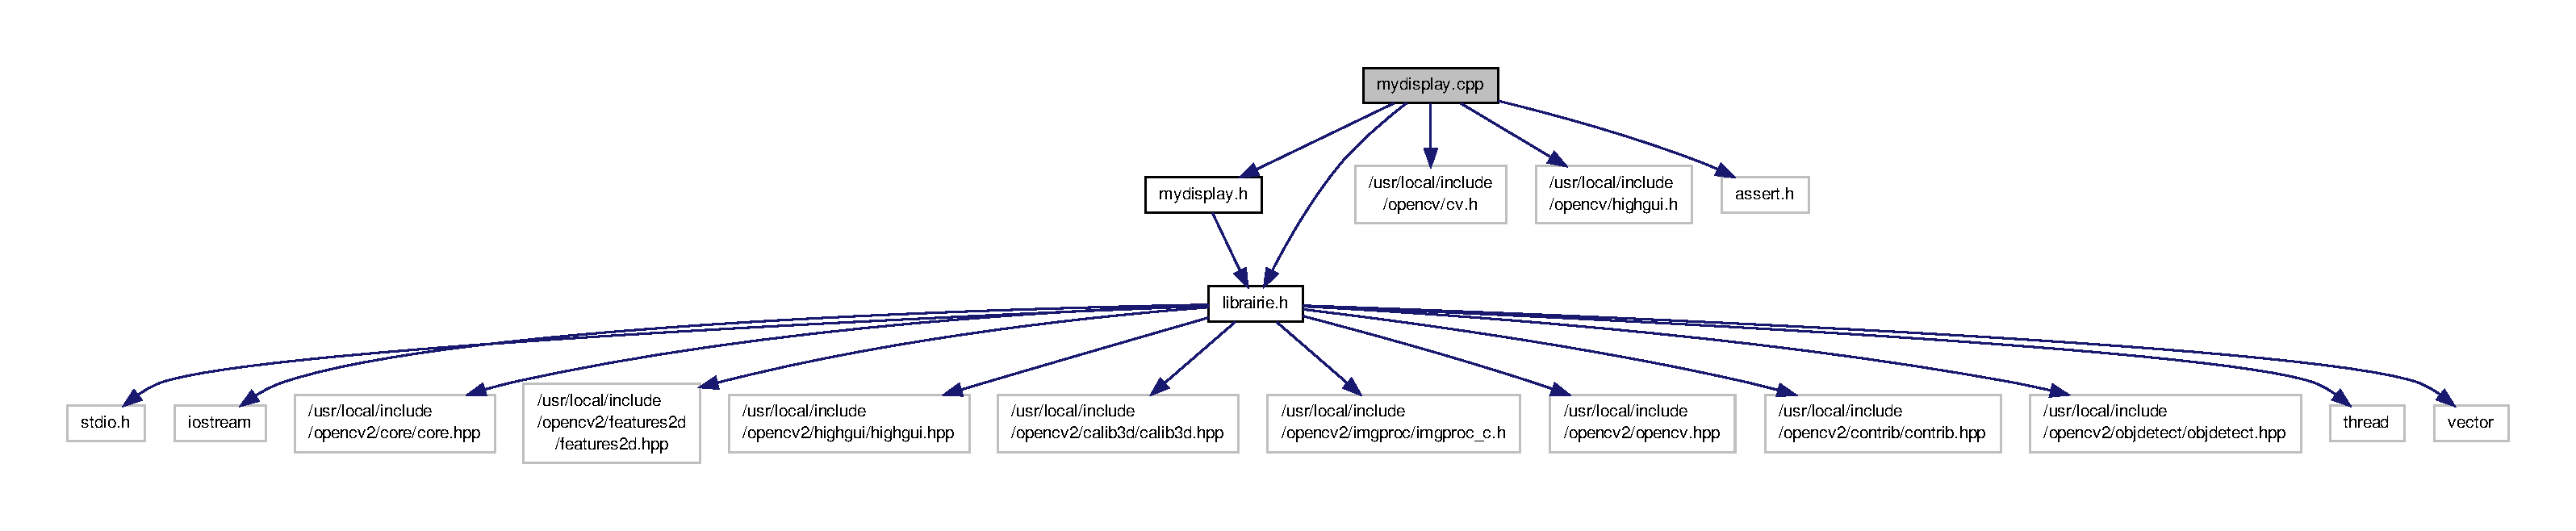
\includegraphics[width=350pt]{mydisplay_8cpp__incl}
\end{center}
\end{figure}
\subsection*{Variables}
\begin{DoxyCompactItemize}
\item 
int \hyperlink{mydisplay_8cpp_ae457e5865ed4e7b5a35200fd4b3b8f47}{threshold\-\_\-select}
\item 
int \hyperlink{mydisplay_8cpp_a040fad353c8bfac3cd8329eb5ea18910}{inversion}
\end{DoxyCompactItemize}


\subsection{Variable Documentation}
\hypertarget{mydisplay_8cpp_a040fad353c8bfac3cd8329eb5ea18910}{\index{mydisplay.\-cpp@{mydisplay.\-cpp}!inversion@{inversion}}
\index{inversion@{inversion}!mydisplay.cpp@{mydisplay.\-cpp}}
\subsubsection[{inversion}]{\setlength{\rightskip}{0pt plus 5cm}int inversion}}\label{mydisplay_8cpp_a040fad353c8bfac3cd8329eb5ea18910}


Definition at line 10 of file mydisplay.\-cpp.

\hypertarget{mydisplay_8cpp_ae457e5865ed4e7b5a35200fd4b3b8f47}{\index{mydisplay.\-cpp@{mydisplay.\-cpp}!threshold\-\_\-select@{threshold\-\_\-select}}
\index{threshold\-\_\-select@{threshold\-\_\-select}!mydisplay.cpp@{mydisplay.\-cpp}}
\subsubsection[{threshold\-\_\-select}]{\setlength{\rightskip}{0pt plus 5cm}int threshold\-\_\-select}}\label{mydisplay_8cpp_ae457e5865ed4e7b5a35200fd4b3b8f47}


Definition at line 9 of file mydisplay.\-cpp.


\hypertarget{mydisplay_8h}{\section{mydisplay.\-h File Reference}
\label{mydisplay_8h}\index{mydisplay.\-h@{mydisplay.\-h}}
}
{\ttfamily \#include \char`\"{}librairie.\-h\char`\"{}}\\*
Include dependency graph for mydisplay.\-h\-:\nopagebreak
\begin{figure}[H]
\begin{center}
\leavevmode
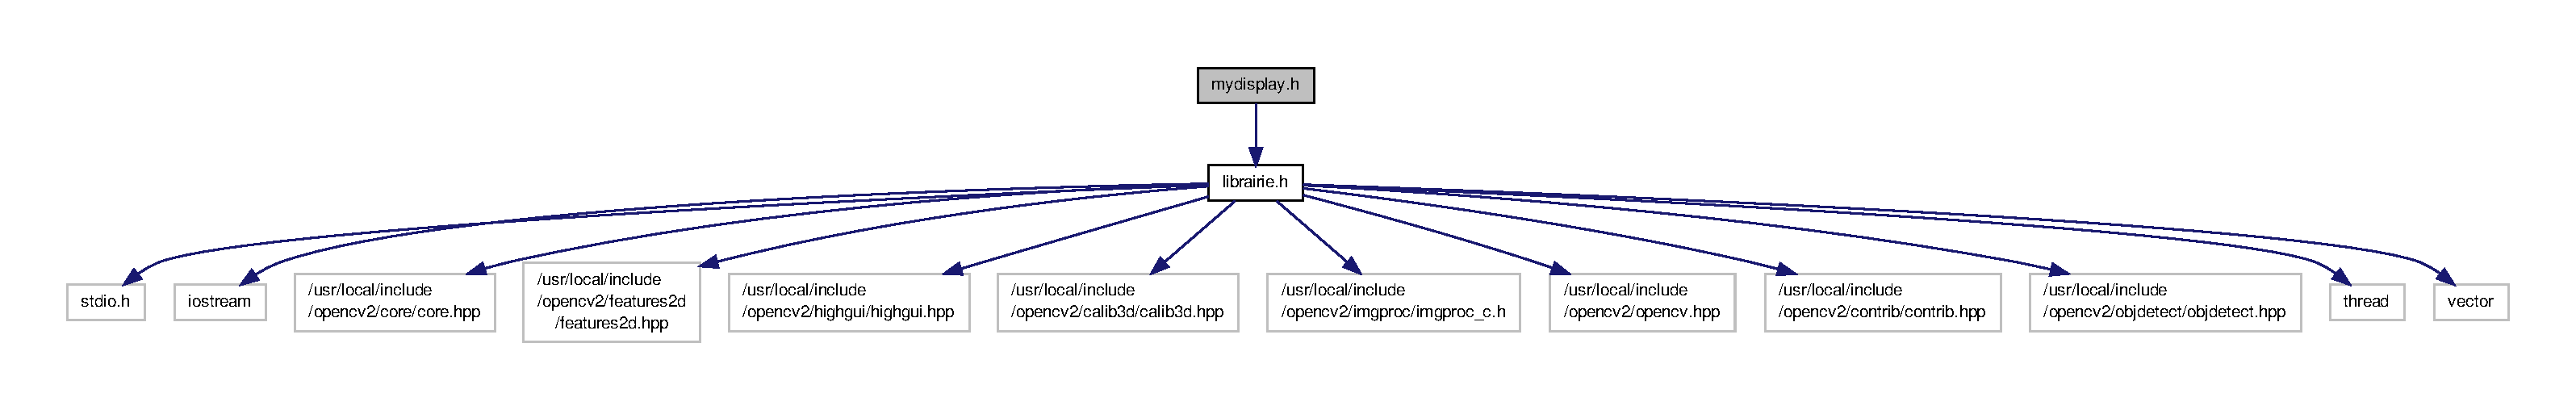
\includegraphics[width=350pt]{mydisplay_8h__incl}
\end{center}
\end{figure}
This graph shows which files directly or indirectly include this file\-:\nopagebreak
\begin{figure}[H]
\begin{center}
\leavevmode
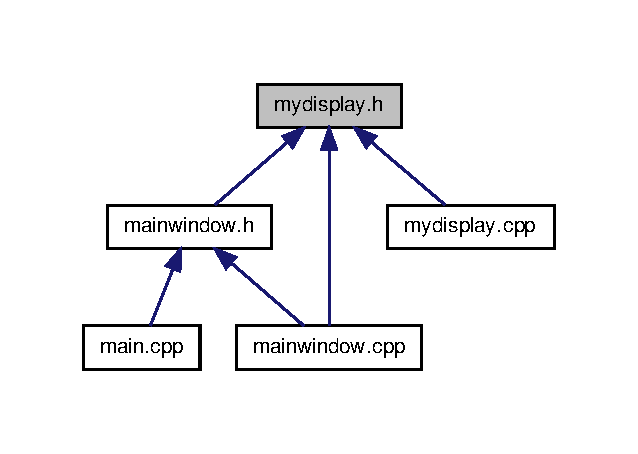
\includegraphics[width=306pt]{mydisplay_8h__dep__incl}
\end{center}
\end{figure}
\subsection*{Classes}
\begin{DoxyCompactItemize}
\item 
class \hyperlink{classMyDisplay}{My\-Display}
\end{DoxyCompactItemize}
\subsection*{Macros}
\begin{DoxyCompactItemize}
\item 
\#define \hyperlink{mydisplay_8h_ad8ce4efaa307683d3d763b37b4711c53}{A\-P\-I}~Q\-T
\end{DoxyCompactItemize}


\subsection{Macro Definition Documentation}
\hypertarget{mydisplay_8h_ad8ce4efaa307683d3d763b37b4711c53}{\index{mydisplay.\-h@{mydisplay.\-h}!A\-P\-I@{A\-P\-I}}
\index{A\-P\-I@{A\-P\-I}!mydisplay.h@{mydisplay.\-h}}
\subsubsection[{A\-P\-I}]{\setlength{\rightskip}{0pt plus 5cm}\#define A\-P\-I~Q\-T}}\label{mydisplay_8h_ad8ce4efaa307683d3d763b37b4711c53}


Definition at line 6 of file mydisplay.\-h.


\hypertarget{nunchuck_8cpp}{\section{nunchuck.\-cpp File Reference}
\label{nunchuck_8cpp}\index{nunchuck.\-cpp@{nunchuck.\-cpp}}
}
{\ttfamily \#include \char`\"{}nunchuck.\-h\char`\"{}}\\*
Include dependency graph for nunchuck.\-cpp\-:\nopagebreak
\begin{figure}[H]
\begin{center}
\leavevmode
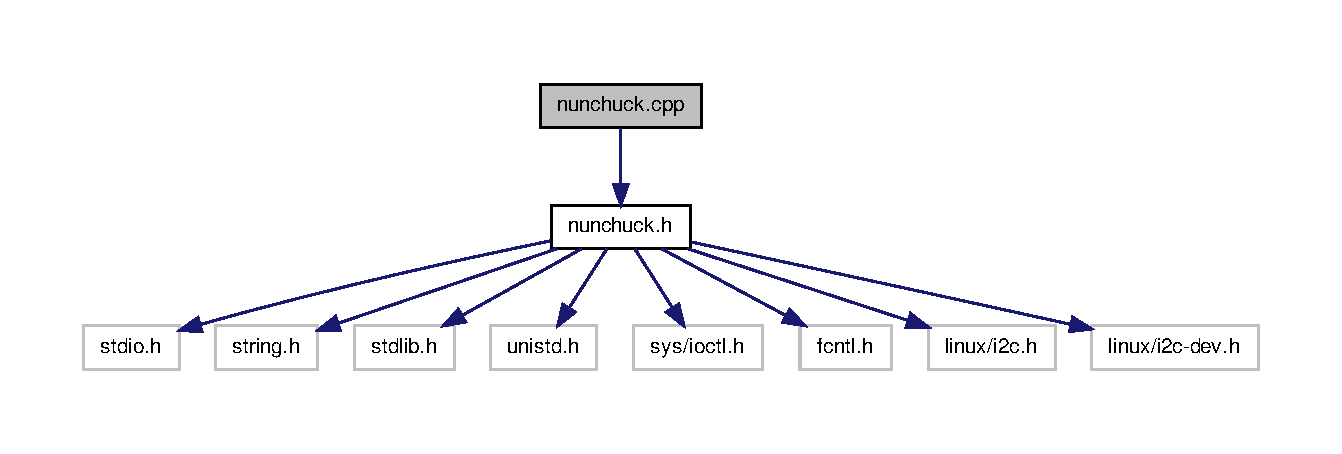
\includegraphics[width=350pt]{nunchuck_8cpp__incl}
\end{center}
\end{figure}

\hypertarget{nunchuck_8h}{\section{nunchuck.\-h File Reference}
\label{nunchuck_8h}\index{nunchuck.\-h@{nunchuck.\-h}}
}
{\ttfamily \#include $<$stdio.\-h$>$}\\*
{\ttfamily \#include $<$string.\-h$>$}\\*
{\ttfamily \#include $<$stdlib.\-h$>$}\\*
{\ttfamily \#include $<$unistd.\-h$>$}\\*
{\ttfamily \#include $<$sys/ioctl.\-h$>$}\\*
{\ttfamily \#include $<$fcntl.\-h$>$}\\*
{\ttfamily \#include $<$linux/i2c.\-h$>$}\\*
{\ttfamily \#include $<$linux/i2c-\/dev.\-h$>$}\\*
Include dependency graph for nunchuck.\-h\-:\nopagebreak
\begin{figure}[H]
\begin{center}
\leavevmode
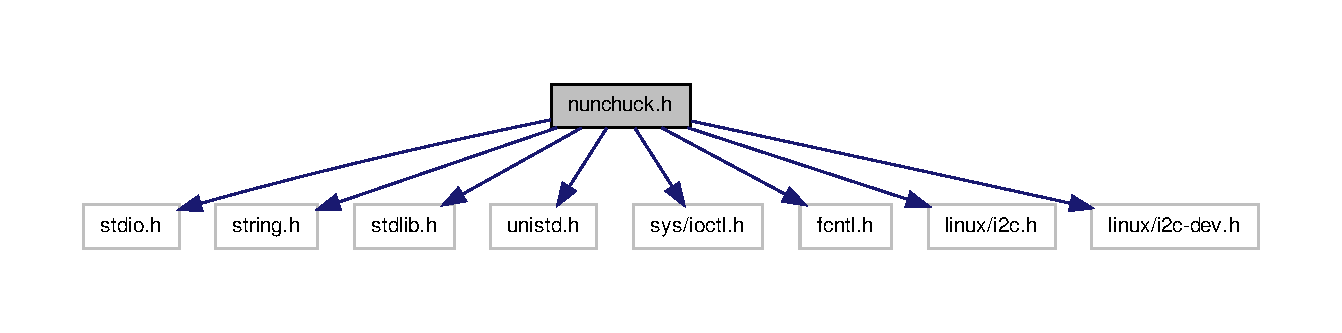
\includegraphics[width=350pt]{nunchuck_8h__incl}
\end{center}
\end{figure}
This graph shows which files directly or indirectly include this file\-:\nopagebreak
\begin{figure}[H]
\begin{center}
\leavevmode
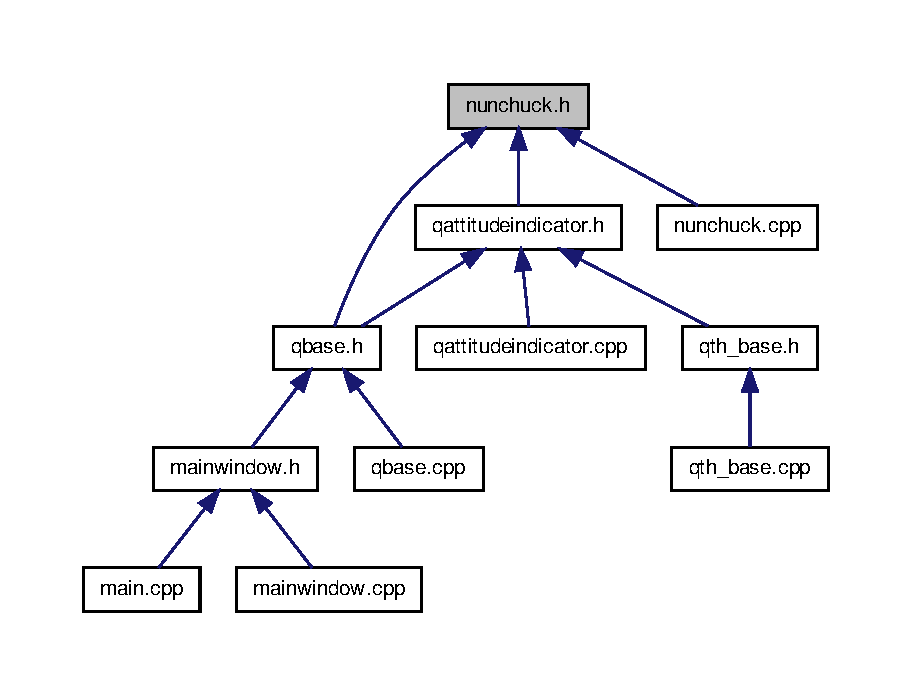
\includegraphics[width=350pt]{nunchuck_8h__dep__incl}
\end{center}
\end{figure}
\subsection*{Classes}
\begin{DoxyCompactItemize}
\item 
class \hyperlink{classNunchuck}{Nunchuck}
\end{DoxyCompactItemize}
\subsection*{Macros}
\begin{DoxyCompactItemize}
\item 
\#define \hyperlink{nunchuck_8h_a0f3e5db0fbc68310b4cdc94e00f10f75}{P\-A\-R\-A\-M\-\_\-\-D\-E\-V\-I\-C\-E\-N\-A\-M\-E\-\_\-\-C\-O\-M\-M\-A\-N\-D\-E}~\char`\"{}/dev/i2c-\/X\char`\"{};
\item 
\#define \hyperlink{nunchuck_8h_abeac51046230d277dc5701b7e45dc88e}{P\-A\-R\-A\-M\-\_\-\-D\-I\-R\-E\-C\-T\-I\-O\-N}~'1'
\item 
\#define \hyperlink{nunchuck_8h_af420e9167d30b82b0f623019d165944a}{P\-A\-R\-A\-M\-\_\-\-A\-L\-T\-I\-T\-U\-D\-E}~'0'
\item 
\#define \hyperlink{nunchuck_8h_ac63506adba6ed764c5061ac249623554}{J\-C\-E\-N\-T\-R\-E}~0
\item 
\#define \hyperlink{nunchuck_8h_abb937f82823e628ca09a026777179226}{J\-D\-R\-O\-I\-T\-E}~1
\item 
\#define \hyperlink{nunchuck_8h_a2948a7fb931671c2935a67be056ec44d}{J\-G\-A\-U\-C\-H\-E}~2
\item 
\#define \hyperlink{nunchuck_8h_a624208e4279eb8508e4d7a4cd1983293}{J\-H\-A\-U\-T}~4
\item 
\#define \hyperlink{nunchuck_8h_ad9a8fe51b03c91dc0256cc7502d450a3}{J\-B\-A\-S}~8
\item 
\#define \hyperlink{nunchuck_8h_a13baf3bab74f21c7050fb8029bf5b871}{J\-D\-R\-O\-I\-T\-E\-\_\-\-M\-A\-X}~16
\item 
\#define \hyperlink{nunchuck_8h_a19f4efb3793bd7fd7da3a60339dc4631}{J\-G\-A\-U\-C\-H\-E\-\_\-\-M\-A\-X}~32
\item 
\#define \hyperlink{nunchuck_8h_a69c726c7ddc8415a81ea58834356ed2b}{J\-H\-A\-U\-T\-\_\-\-M\-A\-X}~64
\item 
\#define \hyperlink{nunchuck_8h_a8bd0c46505c3f0a7d5bc412d8a56d41a}{J\-B\-A\-S\-\_\-\-M\-A\-X}~127
\end{DoxyCompactItemize}


\subsection{Macro Definition Documentation}
\hypertarget{nunchuck_8h_ad9a8fe51b03c91dc0256cc7502d450a3}{\index{nunchuck.\-h@{nunchuck.\-h}!J\-B\-A\-S@{J\-B\-A\-S}}
\index{J\-B\-A\-S@{J\-B\-A\-S}!nunchuck.h@{nunchuck.\-h}}
\subsubsection[{J\-B\-A\-S}]{\setlength{\rightskip}{0pt plus 5cm}\#define J\-B\-A\-S~8}}\label{nunchuck_8h_ad9a8fe51b03c91dc0256cc7502d450a3}


Definition at line 24 of file nunchuck.\-h.



Referenced by Nunchuck\-::\-Decode\-Buffer\-In(), and Q\-Base\-::run().

\hypertarget{nunchuck_8h_a8bd0c46505c3f0a7d5bc412d8a56d41a}{\index{nunchuck.\-h@{nunchuck.\-h}!J\-B\-A\-S\-\_\-\-M\-A\-X@{J\-B\-A\-S\-\_\-\-M\-A\-X}}
\index{J\-B\-A\-S\-\_\-\-M\-A\-X@{J\-B\-A\-S\-\_\-\-M\-A\-X}!nunchuck.h@{nunchuck.\-h}}
\subsubsection[{J\-B\-A\-S\-\_\-\-M\-A\-X}]{\setlength{\rightskip}{0pt plus 5cm}\#define J\-B\-A\-S\-\_\-\-M\-A\-X~127}}\label{nunchuck_8h_a8bd0c46505c3f0a7d5bc412d8a56d41a}


Definition at line 28 of file nunchuck.\-h.



Referenced by Nunchuck\-::\-Decode\-Buffer\-In(), and Q\-Base\-::run().

\hypertarget{nunchuck_8h_ac63506adba6ed764c5061ac249623554}{\index{nunchuck.\-h@{nunchuck.\-h}!J\-C\-E\-N\-T\-R\-E@{J\-C\-E\-N\-T\-R\-E}}
\index{J\-C\-E\-N\-T\-R\-E@{J\-C\-E\-N\-T\-R\-E}!nunchuck.h@{nunchuck.\-h}}
\subsubsection[{J\-C\-E\-N\-T\-R\-E}]{\setlength{\rightskip}{0pt plus 5cm}\#define J\-C\-E\-N\-T\-R\-E~0}}\label{nunchuck_8h_ac63506adba6ed764c5061ac249623554}


Definition at line 20 of file nunchuck.\-h.



Referenced by Nunchuck\-::\-Decode\-Buffer\-In(), and Q\-Base\-::run().

\hypertarget{nunchuck_8h_abb937f82823e628ca09a026777179226}{\index{nunchuck.\-h@{nunchuck.\-h}!J\-D\-R\-O\-I\-T\-E@{J\-D\-R\-O\-I\-T\-E}}
\index{J\-D\-R\-O\-I\-T\-E@{J\-D\-R\-O\-I\-T\-E}!nunchuck.h@{nunchuck.\-h}}
\subsubsection[{J\-D\-R\-O\-I\-T\-E}]{\setlength{\rightskip}{0pt plus 5cm}\#define J\-D\-R\-O\-I\-T\-E~1}}\label{nunchuck_8h_abb937f82823e628ca09a026777179226}


Definition at line 21 of file nunchuck.\-h.



Referenced by Nunchuck\-::\-Decode\-Buffer\-In(), and Q\-Base\-::run().

\hypertarget{nunchuck_8h_a13baf3bab74f21c7050fb8029bf5b871}{\index{nunchuck.\-h@{nunchuck.\-h}!J\-D\-R\-O\-I\-T\-E\-\_\-\-M\-A\-X@{J\-D\-R\-O\-I\-T\-E\-\_\-\-M\-A\-X}}
\index{J\-D\-R\-O\-I\-T\-E\-\_\-\-M\-A\-X@{J\-D\-R\-O\-I\-T\-E\-\_\-\-M\-A\-X}!nunchuck.h@{nunchuck.\-h}}
\subsubsection[{J\-D\-R\-O\-I\-T\-E\-\_\-\-M\-A\-X}]{\setlength{\rightskip}{0pt plus 5cm}\#define J\-D\-R\-O\-I\-T\-E\-\_\-\-M\-A\-X~16}}\label{nunchuck_8h_a13baf3bab74f21c7050fb8029bf5b871}


Definition at line 25 of file nunchuck.\-h.



Referenced by Nunchuck\-::\-Decode\-Buffer\-In(), and Q\-Base\-::run().

\hypertarget{nunchuck_8h_a2948a7fb931671c2935a67be056ec44d}{\index{nunchuck.\-h@{nunchuck.\-h}!J\-G\-A\-U\-C\-H\-E@{J\-G\-A\-U\-C\-H\-E}}
\index{J\-G\-A\-U\-C\-H\-E@{J\-G\-A\-U\-C\-H\-E}!nunchuck.h@{nunchuck.\-h}}
\subsubsection[{J\-G\-A\-U\-C\-H\-E}]{\setlength{\rightskip}{0pt plus 5cm}\#define J\-G\-A\-U\-C\-H\-E~2}}\label{nunchuck_8h_a2948a7fb931671c2935a67be056ec44d}


Definition at line 22 of file nunchuck.\-h.



Referenced by Nunchuck\-::\-Decode\-Buffer\-In(), and Q\-Base\-::run().

\hypertarget{nunchuck_8h_a19f4efb3793bd7fd7da3a60339dc4631}{\index{nunchuck.\-h@{nunchuck.\-h}!J\-G\-A\-U\-C\-H\-E\-\_\-\-M\-A\-X@{J\-G\-A\-U\-C\-H\-E\-\_\-\-M\-A\-X}}
\index{J\-G\-A\-U\-C\-H\-E\-\_\-\-M\-A\-X@{J\-G\-A\-U\-C\-H\-E\-\_\-\-M\-A\-X}!nunchuck.h@{nunchuck.\-h}}
\subsubsection[{J\-G\-A\-U\-C\-H\-E\-\_\-\-M\-A\-X}]{\setlength{\rightskip}{0pt plus 5cm}\#define J\-G\-A\-U\-C\-H\-E\-\_\-\-M\-A\-X~32}}\label{nunchuck_8h_a19f4efb3793bd7fd7da3a60339dc4631}


Definition at line 26 of file nunchuck.\-h.



Referenced by Nunchuck\-::\-Decode\-Buffer\-In(), and Q\-Base\-::run().

\hypertarget{nunchuck_8h_a624208e4279eb8508e4d7a4cd1983293}{\index{nunchuck.\-h@{nunchuck.\-h}!J\-H\-A\-U\-T@{J\-H\-A\-U\-T}}
\index{J\-H\-A\-U\-T@{J\-H\-A\-U\-T}!nunchuck.h@{nunchuck.\-h}}
\subsubsection[{J\-H\-A\-U\-T}]{\setlength{\rightskip}{0pt plus 5cm}\#define J\-H\-A\-U\-T~4}}\label{nunchuck_8h_a624208e4279eb8508e4d7a4cd1983293}


Definition at line 23 of file nunchuck.\-h.



Referenced by Nunchuck\-::\-Decode\-Buffer\-In(), and Q\-Base\-::run().

\hypertarget{nunchuck_8h_a69c726c7ddc8415a81ea58834356ed2b}{\index{nunchuck.\-h@{nunchuck.\-h}!J\-H\-A\-U\-T\-\_\-\-M\-A\-X@{J\-H\-A\-U\-T\-\_\-\-M\-A\-X}}
\index{J\-H\-A\-U\-T\-\_\-\-M\-A\-X@{J\-H\-A\-U\-T\-\_\-\-M\-A\-X}!nunchuck.h@{nunchuck.\-h}}
\subsubsection[{J\-H\-A\-U\-T\-\_\-\-M\-A\-X}]{\setlength{\rightskip}{0pt plus 5cm}\#define J\-H\-A\-U\-T\-\_\-\-M\-A\-X~64}}\label{nunchuck_8h_a69c726c7ddc8415a81ea58834356ed2b}


Definition at line 27 of file nunchuck.\-h.



Referenced by Nunchuck\-::\-Decode\-Buffer\-In(), and Q\-Base\-::run().

\hypertarget{nunchuck_8h_af420e9167d30b82b0f623019d165944a}{\index{nunchuck.\-h@{nunchuck.\-h}!P\-A\-R\-A\-M\-\_\-\-A\-L\-T\-I\-T\-U\-D\-E@{P\-A\-R\-A\-M\-\_\-\-A\-L\-T\-I\-T\-U\-D\-E}}
\index{P\-A\-R\-A\-M\-\_\-\-A\-L\-T\-I\-T\-U\-D\-E@{P\-A\-R\-A\-M\-\_\-\-A\-L\-T\-I\-T\-U\-D\-E}!nunchuck.h@{nunchuck.\-h}}
\subsubsection[{P\-A\-R\-A\-M\-\_\-\-A\-L\-T\-I\-T\-U\-D\-E}]{\setlength{\rightskip}{0pt plus 5cm}\#define P\-A\-R\-A\-M\-\_\-\-A\-L\-T\-I\-T\-U\-D\-E~'0'}}\label{nunchuck_8h_af420e9167d30b82b0f623019d165944a}


Definition at line 18 of file nunchuck.\-h.



Referenced by Q\-Base\-::\-Q\-Base().

\hypertarget{nunchuck_8h_a0f3e5db0fbc68310b4cdc94e00f10f75}{\index{nunchuck.\-h@{nunchuck.\-h}!P\-A\-R\-A\-M\-\_\-\-D\-E\-V\-I\-C\-E\-N\-A\-M\-E\-\_\-\-C\-O\-M\-M\-A\-N\-D\-E@{P\-A\-R\-A\-M\-\_\-\-D\-E\-V\-I\-C\-E\-N\-A\-M\-E\-\_\-\-C\-O\-M\-M\-A\-N\-D\-E}}
\index{P\-A\-R\-A\-M\-\_\-\-D\-E\-V\-I\-C\-E\-N\-A\-M\-E\-\_\-\-C\-O\-M\-M\-A\-N\-D\-E@{P\-A\-R\-A\-M\-\_\-\-D\-E\-V\-I\-C\-E\-N\-A\-M\-E\-\_\-\-C\-O\-M\-M\-A\-N\-D\-E}!nunchuck.h@{nunchuck.\-h}}
\subsubsection[{P\-A\-R\-A\-M\-\_\-\-D\-E\-V\-I\-C\-E\-N\-A\-M\-E\-\_\-\-C\-O\-M\-M\-A\-N\-D\-E}]{\setlength{\rightskip}{0pt plus 5cm}\#define P\-A\-R\-A\-M\-\_\-\-D\-E\-V\-I\-C\-E\-N\-A\-M\-E\-\_\-\-C\-O\-M\-M\-A\-N\-D\-E~\char`\"{}/dev/i2c-\/X\char`\"{};}}\label{nunchuck_8h_a0f3e5db0fbc68310b4cdc94e00f10f75}


Definition at line 16 of file nunchuck.\-h.



Referenced by Nunchuck\-::\-Initialize().

\hypertarget{nunchuck_8h_abeac51046230d277dc5701b7e45dc88e}{\index{nunchuck.\-h@{nunchuck.\-h}!P\-A\-R\-A\-M\-\_\-\-D\-I\-R\-E\-C\-T\-I\-O\-N@{P\-A\-R\-A\-M\-\_\-\-D\-I\-R\-E\-C\-T\-I\-O\-N}}
\index{P\-A\-R\-A\-M\-\_\-\-D\-I\-R\-E\-C\-T\-I\-O\-N@{P\-A\-R\-A\-M\-\_\-\-D\-I\-R\-E\-C\-T\-I\-O\-N}!nunchuck.h@{nunchuck.\-h}}
\subsubsection[{P\-A\-R\-A\-M\-\_\-\-D\-I\-R\-E\-C\-T\-I\-O\-N}]{\setlength{\rightskip}{0pt plus 5cm}\#define P\-A\-R\-A\-M\-\_\-\-D\-I\-R\-E\-C\-T\-I\-O\-N~'1'}}\label{nunchuck_8h_abeac51046230d277dc5701b7e45dc88e}


Definition at line 17 of file nunchuck.\-h.



Referenced by Q\-Base\-::\-Q\-Base().


\hypertarget{qattitudeindicator_8cpp}{\section{qattitudeindicator.\-cpp File Reference}
\label{qattitudeindicator_8cpp}\index{qattitudeindicator.\-cpp@{qattitudeindicator.\-cpp}}
}
{\ttfamily \#include $<$Qt\-Gui$>$}\\*
{\ttfamily \#include $<$Q\-Debug$>$}\\*
{\ttfamily \#include \char`\"{}qattitudeindicator.\-h\char`\"{}}\\*
{\ttfamily \#include $<$fstream$>$}\\*
{\ttfamily \#include $<$sstream$>$}\\*
Include dependency graph for qattitudeindicator.\-cpp\-:\nopagebreak
\begin{figure}[H]
\begin{center}
\leavevmode
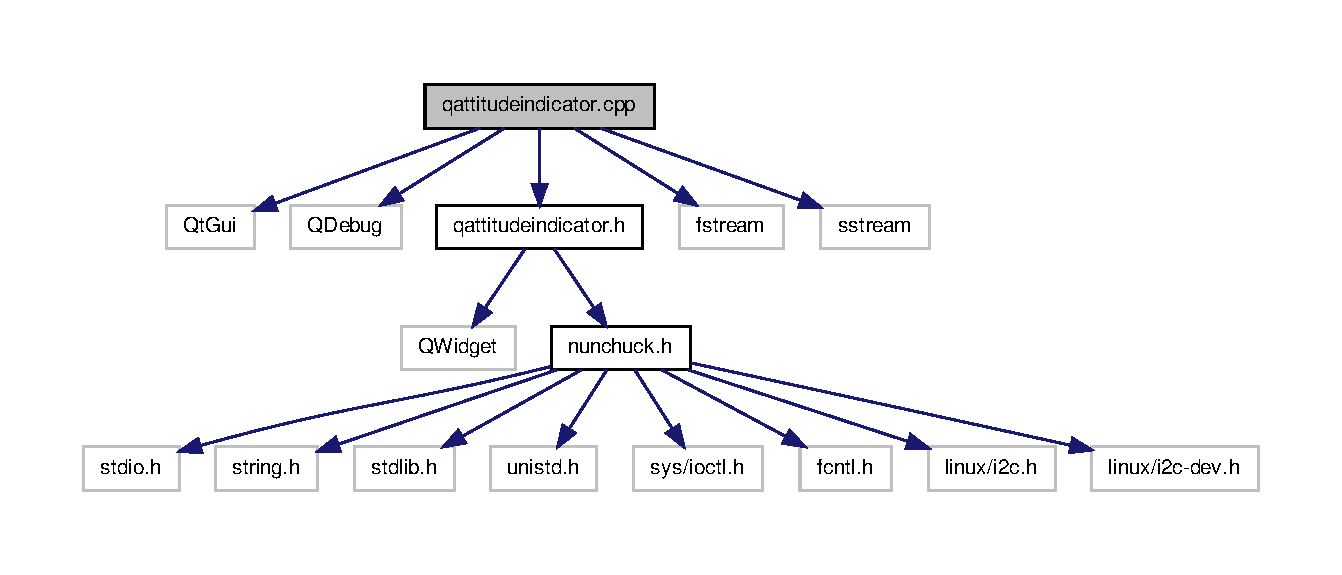
\includegraphics[width=350pt]{qattitudeindicator_8cpp__incl}
\end{center}
\end{figure}
\subsection*{Variables}
\begin{DoxyCompactItemize}
\item 
qreal \hyperlink{qattitudeindicator_8cpp_a2f4f279d4d5470569f9b4d6db0e913c3}{defaults\-Roll\-Rotate} \mbox{[}\hyperlink{qattitudeindicator_8h_a533fb9cffe544953a1e34ef3ca40cd9aae68d533445c770721902ff44425e6cda}{numb\-Roll\-Line}\mbox{]} = \{270.\-0,30.\-0,15.\-0,15.\-0,10.\-0,10.\-0,10.\-0,10.\-0,10.\-0,10.\-0,15.\-0,15.\-0,30.\-0\}
\item 
\hyperlink{qattitudeindicator_8h_a343e47e8a321f67b38cb4522cb218c94}{E\-N\-\_\-\-T\-Y\-P\-E\-S\-\_\-\-A\-T\-T\-I\-T\-U\-D\-E} \hyperlink{qattitudeindicator_8cpp_a3e866b9c9b8bde50fd68030b49604a15}{defaults\-Type\-Roll} \mbox{[}\hyperlink{qattitudeindicator_8h_a533fb9cffe544953a1e34ef3ca40cd9aae68d533445c770721902ff44425e6cda}{numb\-Roll\-Line}\mbox{]}
\item 
\hyperlink{qattitudeindicator_8h_a343e47e8a321f67b38cb4522cb218c94}{E\-N\-\_\-\-T\-Y\-P\-E\-S\-\_\-\-A\-T\-T\-I\-T\-U\-D\-E} \hyperlink{qattitudeindicator_8cpp_aeb622d2485fb495e7b9864ca595af136}{defaults\-Type\-Pitch} \mbox{[}\hyperlink{qattitudeindicator_8h_a533fb9cffe544953a1e34ef3ca40cd9aaf86b1d616737ab90eedf9d904603bbc7}{numb\-Pitch\-Line}\mbox{]}
\end{DoxyCompactItemize}


\subsection{Variable Documentation}
\hypertarget{qattitudeindicator_8cpp_a2f4f279d4d5470569f9b4d6db0e913c3}{\index{qattitudeindicator.\-cpp@{qattitudeindicator.\-cpp}!defaults\-Roll\-Rotate@{defaults\-Roll\-Rotate}}
\index{defaults\-Roll\-Rotate@{defaults\-Roll\-Rotate}!qattitudeindicator.cpp@{qattitudeindicator.\-cpp}}
\subsubsection[{defaults\-Roll\-Rotate}]{\setlength{\rightskip}{0pt plus 5cm}qreal defaults\-Roll\-Rotate\mbox{[}{\bf numb\-Roll\-Line}\mbox{]} = \{270.\-0,30.\-0,15.\-0,15.\-0,10.\-0,10.\-0,10.\-0,10.\-0,10.\-0,10.\-0,15.\-0,15.\-0,30.\-0\}}}\label{qattitudeindicator_8cpp_a2f4f279d4d5470569f9b4d6db0e913c3}


Definition at line 7 of file qattitudeindicator.\-cpp.



Referenced by q\-Attitude\-Indicator\-::q\-Attitude\-Indicator().

\hypertarget{qattitudeindicator_8cpp_aeb622d2485fb495e7b9864ca595af136}{\index{qattitudeindicator.\-cpp@{qattitudeindicator.\-cpp}!defaults\-Type\-Pitch@{defaults\-Type\-Pitch}}
\index{defaults\-Type\-Pitch@{defaults\-Type\-Pitch}!qattitudeindicator.cpp@{qattitudeindicator.\-cpp}}
\subsubsection[{defaults\-Type\-Pitch}]{\setlength{\rightskip}{0pt plus 5cm}{\bf E\-N\-\_\-\-T\-Y\-P\-E\-S\-\_\-\-A\-T\-T\-I\-T\-U\-D\-E} defaults\-Type\-Pitch\mbox{[}{\bf numb\-Pitch\-Line}\mbox{]}}}\label{qattitudeindicator_8cpp_aeb622d2485fb495e7b9864ca595af136}
{\bfseries Initial value\-:}
\begin{DoxyCode}
 \{ \hyperlink{qattitudeindicator_8h_a9e6157b3f1ec4c2db1f8a664f6347784a0369563b4b4cadd85d30f57de453ffb8}{normalPitchLine},\hyperlink{qattitudeindicator_8h_a9e6157b3f1ec4c2db1f8a664f6347784a27d8d9b85932b52acefebc1edaebac45}{smallPitchLine} ,\hyperlink{qattitudeindicator_8h_a9e6157b3f1ec4c2db1f8a664f6347784a0369563b4b4cadd85d30f57de453ffb8}{normalPitchLine}
      ,\hyperlink{qattitudeindicator_8h_a9e6157b3f1ec4c2db1f8a664f6347784a27d8d9b85932b52acefebc1edaebac45}{smallPitchLine},
                                                       \hyperlink{qattitudeindicator_8h_a9e6157b3f1ec4c2db1f8a664f6347784a27d8d9b85932b52acefebc1edaebac45}{smallPitchLine}
       ,\hyperlink{qattitudeindicator_8h_a9e6157b3f1ec4c2db1f8a664f6347784a0369563b4b4cadd85d30f57de453ffb8}{normalPitchLine},\hyperlink{qattitudeindicator_8h_a9e6157b3f1ec4c2db1f8a664f6347784a27d8d9b85932b52acefebc1edaebac45}{smallPitchLine}, normalPitchLine\}
\end{DoxyCode}


Definition at line 13 of file qattitudeindicator.\-cpp.



Referenced by q\-Attitude\-Indicator\-::q\-Attitude\-Indicator(), and q\-Attitude\-Indicator\-::resize\-Event().

\hypertarget{qattitudeindicator_8cpp_a3e866b9c9b8bde50fd68030b49604a15}{\index{qattitudeindicator.\-cpp@{qattitudeindicator.\-cpp}!defaults\-Type\-Roll@{defaults\-Type\-Roll}}
\index{defaults\-Type\-Roll@{defaults\-Type\-Roll}!qattitudeindicator.cpp@{qattitudeindicator.\-cpp}}
\subsubsection[{defaults\-Type\-Roll}]{\setlength{\rightskip}{0pt plus 5cm}{\bf E\-N\-\_\-\-T\-Y\-P\-E\-S\-\_\-\-A\-T\-T\-I\-T\-U\-D\-E} defaults\-Type\-Roll\mbox{[}{\bf numb\-Roll\-Line}\mbox{]}}}\label{qattitudeindicator_8cpp_a3e866b9c9b8bde50fd68030b49604a15}
{\bfseries Initial value\-:}
\begin{DoxyCode}
 \{ \hyperlink{qattitudeindicator_8h_a9e6157b3f1ec4c2db1f8a664f6347784a282d8d28348dde5a5265aa34d80a0f01}{normalRollLine},\hyperlink{qattitudeindicator_8h_a9e6157b3f1ec4c2db1f8a664f6347784a282d8d28348dde5a5265aa34d80a0f01}{normalRollLine} ,\hyperlink{qattitudeindicator_8h_a9e6157b3f1ec4c2db1f8a664f6347784a24e88cb96dabfbd43afd71b24529147a}{smallRollLine}
       ,\hyperlink{qattitudeindicator_8h_a9e6157b3f1ec4c2db1f8a664f6347784a282d8d28348dde5a5265aa34d80a0f01}{normalRollLine},
                                                     \hyperlink{qattitudeindicator_8h_a9e6157b3f1ec4c2db1f8a664f6347784a24e88cb96dabfbd43afd71b24529147a}{smallRollLine}
       ,\hyperlink{qattitudeindicator_8h_a9e6157b3f1ec4c2db1f8a664f6347784a24e88cb96dabfbd43afd71b24529147a}{smallRollLine}  ,\hyperlink{qattitudeindicator_8h_a9e6157b3f1ec4c2db1f8a664f6347784a282d8d28348dde5a5265aa34d80a0f01}{normalRollLine},\hyperlink{qattitudeindicator_8h_a9e6157b3f1ec4c2db1f8a664f6347784a24e88cb96dabfbd43afd71b24529147a}{smallRollLine}
      ,
                                                     \hyperlink{qattitudeindicator_8h_a9e6157b3f1ec4c2db1f8a664f6347784a24e88cb96dabfbd43afd71b24529147a}{smallRollLine}
       ,\hyperlink{qattitudeindicator_8h_a9e6157b3f1ec4c2db1f8a664f6347784a282d8d28348dde5a5265aa34d80a0f01}{normalRollLine} ,\hyperlink{qattitudeindicator_8h_a9e6157b3f1ec4c2db1f8a664f6347784a24e88cb96dabfbd43afd71b24529147a}{smallRollLine} ,\hyperlink{qattitudeindicator_8h_a9e6157b3f1ec4c2db1f8a664f6347784a282d8d28348dde5a5265aa34d80a0f01}{normalRollLine}
      ,
                                                     normalRollLine \}
\end{DoxyCode}


Definition at line 8 of file qattitudeindicator.\-cpp.



Referenced by q\-Attitude\-Indicator\-::q\-Attitude\-Indicator(), and q\-Attitude\-Indicator\-::resize\-Event().


\hypertarget{qattitudeindicator_8h}{\section{qattitudeindicator.\-h File Reference}
\label{qattitudeindicator_8h}\index{qattitudeindicator.\-h@{qattitudeindicator.\-h}}
}
{\ttfamily \#include $<$Q\-Widget$>$}\\*
{\ttfamily \#include $<$nunchuck.\-h$>$}\\*
Include dependency graph for qattitudeindicator.\-h\-:\nopagebreak
\begin{figure}[H]
\begin{center}
\leavevmode
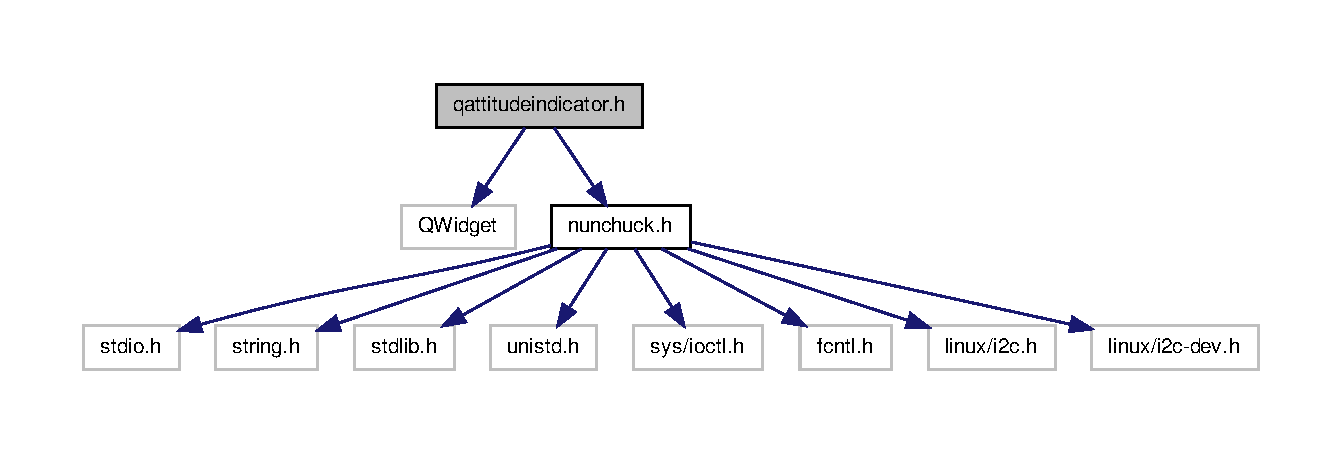
\includegraphics[width=350pt]{qattitudeindicator_8h__incl}
\end{center}
\end{figure}
This graph shows which files directly or indirectly include this file\-:\nopagebreak
\begin{figure}[H]
\begin{center}
\leavevmode
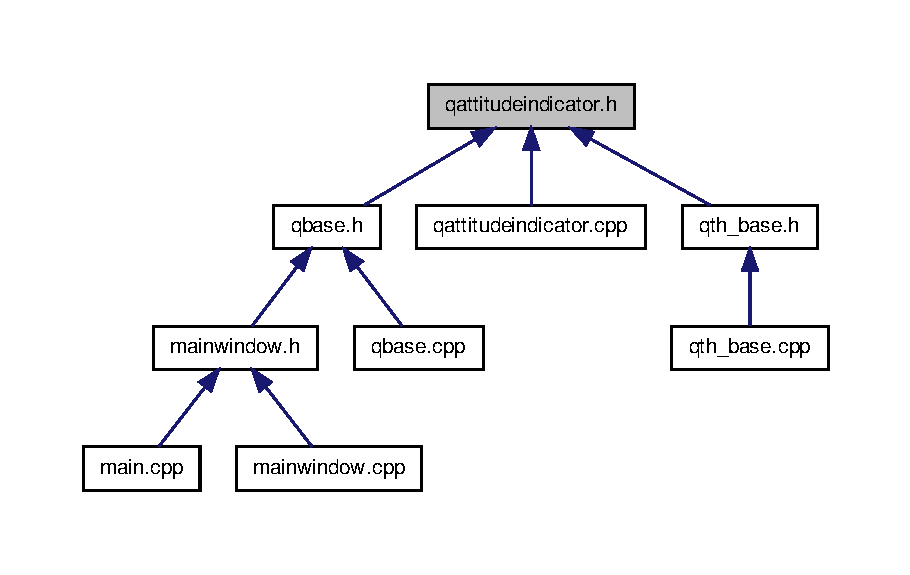
\includegraphics[width=350pt]{qattitudeindicator_8h__dep__incl}
\end{center}
\end{figure}
\subsection*{Classes}
\begin{DoxyCompactItemize}
\item 
class \hyperlink{classqAttitudeIndicator}{q\-Attitude\-Indicator}
\end{DoxyCompactItemize}
\subsection*{Typedefs}
\begin{DoxyCompactItemize}
\item 
typedef enum \\*
\hyperlink{qattitudeindicator_8h_a533fb9cffe544953a1e34ef3ca40cd9a}{\-\_\-en\-\_\-global\-\_\-definitions\-\_\-} \hyperlink{qattitudeindicator_8h_ab50d742f216e5b7673e7eb4bddd3c8d2}{E\-N\-\_\-\-G\-L\-O\-A\-B\-L\-\_\-\-D\-E\-F\-I\-N\-I\-T\-I\-O\-N\-S}
\item 
typedef enum \hyperlink{qattitudeindicator_8h_a9e6157b3f1ec4c2db1f8a664f6347784}{\-\_\-en\-\_\-types\-\_\-attitude\-\_\-} \hyperlink{qattitudeindicator_8h_a343e47e8a321f67b38cb4522cb218c94}{E\-N\-\_\-\-T\-Y\-P\-E\-S\-\_\-\-A\-T\-T\-I\-T\-U\-D\-E}
\end{DoxyCompactItemize}
\subsection*{Enumerations}
\begin{DoxyCompactItemize}
\item 
enum \hyperlink{qattitudeindicator_8h_a533fb9cffe544953a1e34ef3ca40cd9a}{\-\_\-en\-\_\-global\-\_\-definitions\-\_\-} \{ \hyperlink{qattitudeindicator_8h_a533fb9cffe544953a1e34ef3ca40cd9aa7c4896a6b7e0383b6dc1e1186a186c09}{size\-Max} =  600, 
\hyperlink{qattitudeindicator_8h_a533fb9cffe544953a1e34ef3ca40cd9aa467c2cfbbeb81431d3520b2a334cbec1}{size\-Min} =  200, 
\hyperlink{qattitudeindicator_8h_a533fb9cffe544953a1e34ef3ca40cd9aae68d533445c770721902ff44425e6cda}{numb\-Roll\-Line} =  13, 
\hyperlink{qattitudeindicator_8h_a533fb9cffe544953a1e34ef3ca40cd9aaf86b1d616737ab90eedf9d904603bbc7}{numb\-Pitch\-Line} = 8
 \}
\item 
enum \hyperlink{qattitudeindicator_8h_a9e6157b3f1ec4c2db1f8a664f6347784}{\-\_\-en\-\_\-types\-\_\-attitude\-\_\-} \{ \hyperlink{qattitudeindicator_8h_a9e6157b3f1ec4c2db1f8a664f6347784a24e88cb96dabfbd43afd71b24529147a}{small\-Roll\-Line} =  0, 
\hyperlink{qattitudeindicator_8h_a9e6157b3f1ec4c2db1f8a664f6347784a282d8d28348dde5a5265aa34d80a0f01}{normal\-Roll\-Line}, 
\hyperlink{qattitudeindicator_8h_a9e6157b3f1ec4c2db1f8a664f6347784a27d8d9b85932b52acefebc1edaebac45}{small\-Pitch\-Line}, 
\hyperlink{qattitudeindicator_8h_a9e6157b3f1ec4c2db1f8a664f6347784a0369563b4b4cadd85d30f57de453ffb8}{normal\-Pitch\-Line}
 \}
\end{DoxyCompactItemize}


\subsection{Typedef Documentation}
\hypertarget{qattitudeindicator_8h_ab50d742f216e5b7673e7eb4bddd3c8d2}{\index{qattitudeindicator.\-h@{qattitudeindicator.\-h}!E\-N\-\_\-\-G\-L\-O\-A\-B\-L\-\_\-\-D\-E\-F\-I\-N\-I\-T\-I\-O\-N\-S@{E\-N\-\_\-\-G\-L\-O\-A\-B\-L\-\_\-\-D\-E\-F\-I\-N\-I\-T\-I\-O\-N\-S}}
\index{E\-N\-\_\-\-G\-L\-O\-A\-B\-L\-\_\-\-D\-E\-F\-I\-N\-I\-T\-I\-O\-N\-S@{E\-N\-\_\-\-G\-L\-O\-A\-B\-L\-\_\-\-D\-E\-F\-I\-N\-I\-T\-I\-O\-N\-S}!qattitudeindicator.h@{qattitudeindicator.\-h}}
\subsubsection[{E\-N\-\_\-\-G\-L\-O\-A\-B\-L\-\_\-\-D\-E\-F\-I\-N\-I\-T\-I\-O\-N\-S}]{\setlength{\rightskip}{0pt plus 5cm}typedef enum {\bf \-\_\-en\-\_\-global\-\_\-definitions\-\_\-}  {\bf E\-N\-\_\-\-G\-L\-O\-A\-B\-L\-\_\-\-D\-E\-F\-I\-N\-I\-T\-I\-O\-N\-S}}}\label{qattitudeindicator_8h_ab50d742f216e5b7673e7eb4bddd3c8d2}
\hypertarget{qattitudeindicator_8h_a343e47e8a321f67b38cb4522cb218c94}{\index{qattitudeindicator.\-h@{qattitudeindicator.\-h}!E\-N\-\_\-\-T\-Y\-P\-E\-S\-\_\-\-A\-T\-T\-I\-T\-U\-D\-E@{E\-N\-\_\-\-T\-Y\-P\-E\-S\-\_\-\-A\-T\-T\-I\-T\-U\-D\-E}}
\index{E\-N\-\_\-\-T\-Y\-P\-E\-S\-\_\-\-A\-T\-T\-I\-T\-U\-D\-E@{E\-N\-\_\-\-T\-Y\-P\-E\-S\-\_\-\-A\-T\-T\-I\-T\-U\-D\-E}!qattitudeindicator.h@{qattitudeindicator.\-h}}
\subsubsection[{E\-N\-\_\-\-T\-Y\-P\-E\-S\-\_\-\-A\-T\-T\-I\-T\-U\-D\-E}]{\setlength{\rightskip}{0pt plus 5cm}typedef enum {\bf \-\_\-en\-\_\-types\-\_\-attitude\-\_\-}  {\bf E\-N\-\_\-\-T\-Y\-P\-E\-S\-\_\-\-A\-T\-T\-I\-T\-U\-D\-E}}}\label{qattitudeindicator_8h_a343e47e8a321f67b38cb4522cb218c94}


\subsection{Enumeration Type Documentation}
\hypertarget{qattitudeindicator_8h_a533fb9cffe544953a1e34ef3ca40cd9a}{\index{qattitudeindicator.\-h@{qattitudeindicator.\-h}!\-\_\-en\-\_\-global\-\_\-definitions\-\_\-@{\-\_\-en\-\_\-global\-\_\-definitions\-\_\-}}
\index{\-\_\-en\-\_\-global\-\_\-definitions\-\_\-@{\-\_\-en\-\_\-global\-\_\-definitions\-\_\-}!qattitudeindicator.h@{qattitudeindicator.\-h}}
\subsubsection[{\-\_\-en\-\_\-global\-\_\-definitions\-\_\-}]{\setlength{\rightskip}{0pt plus 5cm}enum {\bf \-\_\-en\-\_\-global\-\_\-definitions\-\_\-}}}\label{qattitudeindicator_8h_a533fb9cffe544953a1e34ef3ca40cd9a}
\begin{Desc}
\item[Enumerator\-: ]\par
\begin{description}
\index{size\-Max@{size\-Max}!qattitudeindicator.\-h@{qattitudeindicator.\-h}}\index{qattitudeindicator.\-h@{qattitudeindicator.\-h}!size\-Max@{size\-Max}}\item[{\em 
\hypertarget{qattitudeindicator_8h_a533fb9cffe544953a1e34ef3ca40cd9aa7c4896a6b7e0383b6dc1e1186a186c09}{size\-Max}\label{qattitudeindicator_8h_a533fb9cffe544953a1e34ef3ca40cd9aa7c4896a6b7e0383b6dc1e1186a186c09}
}]\index{size\-Min@{size\-Min}!qattitudeindicator.\-h@{qattitudeindicator.\-h}}\index{qattitudeindicator.\-h@{qattitudeindicator.\-h}!size\-Min@{size\-Min}}\item[{\em 
\hypertarget{qattitudeindicator_8h_a533fb9cffe544953a1e34ef3ca40cd9aa467c2cfbbeb81431d3520b2a334cbec1}{size\-Min}\label{qattitudeindicator_8h_a533fb9cffe544953a1e34ef3ca40cd9aa467c2cfbbeb81431d3520b2a334cbec1}
}]\index{numb\-Roll\-Line@{numb\-Roll\-Line}!qattitudeindicator.\-h@{qattitudeindicator.\-h}}\index{qattitudeindicator.\-h@{qattitudeindicator.\-h}!numb\-Roll\-Line@{numb\-Roll\-Line}}\item[{\em 
\hypertarget{qattitudeindicator_8h_a533fb9cffe544953a1e34ef3ca40cd9aae68d533445c770721902ff44425e6cda}{numb\-Roll\-Line}\label{qattitudeindicator_8h_a533fb9cffe544953a1e34ef3ca40cd9aae68d533445c770721902ff44425e6cda}
}]\index{numb\-Pitch\-Line@{numb\-Pitch\-Line}!qattitudeindicator.\-h@{qattitudeindicator.\-h}}\index{qattitudeindicator.\-h@{qattitudeindicator.\-h}!numb\-Pitch\-Line@{numb\-Pitch\-Line}}\item[{\em 
\hypertarget{qattitudeindicator_8h_a533fb9cffe544953a1e34ef3ca40cd9aaf86b1d616737ab90eedf9d904603bbc7}{numb\-Pitch\-Line}\label{qattitudeindicator_8h_a533fb9cffe544953a1e34ef3ca40cd9aaf86b1d616737ab90eedf9d904603bbc7}
}]\end{description}
\end{Desc}



Definition at line 7 of file qattitudeindicator.\-h.


\begin{DoxyCode}
\{
    \hyperlink{qattitudeindicator_8h_a533fb9cffe544953a1e34ef3ca40cd9aa7c4896a6b7e0383b6dc1e1186a186c09}{sizeMax} = 600,
    \hyperlink{qattitudeindicator_8h_a533fb9cffe544953a1e34ef3ca40cd9aa467c2cfbbeb81431d3520b2a334cbec1}{sizeMin} = 200,
    \hyperlink{qattitudeindicator_8h_a533fb9cffe544953a1e34ef3ca40cd9aae68d533445c770721902ff44425e6cda}{numbRollLine} = 13,
    \hyperlink{qattitudeindicator_8h_a533fb9cffe544953a1e34ef3ca40cd9aaf86b1d616737ab90eedf9d904603bbc7}{numbPitchLine} =8
\} \hyperlink{qattitudeindicator_8h_ab50d742f216e5b7673e7eb4bddd3c8d2}{EN\_GLOABL\_DEFINITIONS};
\end{DoxyCode}
\hypertarget{qattitudeindicator_8h_a9e6157b3f1ec4c2db1f8a664f6347784}{\index{qattitudeindicator.\-h@{qattitudeindicator.\-h}!\-\_\-en\-\_\-types\-\_\-attitude\-\_\-@{\-\_\-en\-\_\-types\-\_\-attitude\-\_\-}}
\index{\-\_\-en\-\_\-types\-\_\-attitude\-\_\-@{\-\_\-en\-\_\-types\-\_\-attitude\-\_\-}!qattitudeindicator.h@{qattitudeindicator.\-h}}
\subsubsection[{\-\_\-en\-\_\-types\-\_\-attitude\-\_\-}]{\setlength{\rightskip}{0pt plus 5cm}enum {\bf \-\_\-en\-\_\-types\-\_\-attitude\-\_\-}}}\label{qattitudeindicator_8h_a9e6157b3f1ec4c2db1f8a664f6347784}
\begin{Desc}
\item[Enumerator\-: ]\par
\begin{description}
\index{small\-Roll\-Line@{small\-Roll\-Line}!qattitudeindicator.\-h@{qattitudeindicator.\-h}}\index{qattitudeindicator.\-h@{qattitudeindicator.\-h}!small\-Roll\-Line@{small\-Roll\-Line}}\item[{\em 
\hypertarget{qattitudeindicator_8h_a9e6157b3f1ec4c2db1f8a664f6347784a24e88cb96dabfbd43afd71b24529147a}{small\-Roll\-Line}\label{qattitudeindicator_8h_a9e6157b3f1ec4c2db1f8a664f6347784a24e88cb96dabfbd43afd71b24529147a}
}]\index{normal\-Roll\-Line@{normal\-Roll\-Line}!qattitudeindicator.\-h@{qattitudeindicator.\-h}}\index{qattitudeindicator.\-h@{qattitudeindicator.\-h}!normal\-Roll\-Line@{normal\-Roll\-Line}}\item[{\em 
\hypertarget{qattitudeindicator_8h_a9e6157b3f1ec4c2db1f8a664f6347784a282d8d28348dde5a5265aa34d80a0f01}{normal\-Roll\-Line}\label{qattitudeindicator_8h_a9e6157b3f1ec4c2db1f8a664f6347784a282d8d28348dde5a5265aa34d80a0f01}
}]\index{small\-Pitch\-Line@{small\-Pitch\-Line}!qattitudeindicator.\-h@{qattitudeindicator.\-h}}\index{qattitudeindicator.\-h@{qattitudeindicator.\-h}!small\-Pitch\-Line@{small\-Pitch\-Line}}\item[{\em 
\hypertarget{qattitudeindicator_8h_a9e6157b3f1ec4c2db1f8a664f6347784a27d8d9b85932b52acefebc1edaebac45}{small\-Pitch\-Line}\label{qattitudeindicator_8h_a9e6157b3f1ec4c2db1f8a664f6347784a27d8d9b85932b52acefebc1edaebac45}
}]\index{normal\-Pitch\-Line@{normal\-Pitch\-Line}!qattitudeindicator.\-h@{qattitudeindicator.\-h}}\index{qattitudeindicator.\-h@{qattitudeindicator.\-h}!normal\-Pitch\-Line@{normal\-Pitch\-Line}}\item[{\em 
\hypertarget{qattitudeindicator_8h_a9e6157b3f1ec4c2db1f8a664f6347784a0369563b4b4cadd85d30f57de453ffb8}{normal\-Pitch\-Line}\label{qattitudeindicator_8h_a9e6157b3f1ec4c2db1f8a664f6347784a0369563b4b4cadd85d30f57de453ffb8}
}]\end{description}
\end{Desc}



Definition at line 15 of file qattitudeindicator.\-h.


\begin{DoxyCode}
\{
    \hyperlink{qattitudeindicator_8h_a9e6157b3f1ec4c2db1f8a664f6347784a24e88cb96dabfbd43afd71b24529147a}{smallRollLine} = 0,
    \hyperlink{qattitudeindicator_8h_a9e6157b3f1ec4c2db1f8a664f6347784a282d8d28348dde5a5265aa34d80a0f01}{normalRollLine},
    \hyperlink{qattitudeindicator_8h_a9e6157b3f1ec4c2db1f8a664f6347784a27d8d9b85932b52acefebc1edaebac45}{smallPitchLine},
    \hyperlink{qattitudeindicator_8h_a9e6157b3f1ec4c2db1f8a664f6347784a0369563b4b4cadd85d30f57de453ffb8}{normalPitchLine}
\} \hyperlink{qattitudeindicator_8h_a343e47e8a321f67b38cb4522cb218c94}{EN\_TYPES\_ATTITUDE};
\end{DoxyCode}

\hypertarget{qbase_8cpp}{\section{qbase.\-cpp File Reference}
\label{qbase_8cpp}\index{qbase.\-cpp@{qbase.\-cpp}}
}
{\ttfamily \#include \char`\"{}qbase.\-h\char`\"{}}\\*
{\ttfamily \#include \char`\"{}stdio.\-h\char`\"{}}\\*
{\ttfamily \#include $<$Q\-Time$>$}\\*
{\ttfamily \#include $<$fstream$>$}\\*
Include dependency graph for qbase.\-cpp\-:\nopagebreak
\begin{figure}[H]
\begin{center}
\leavevmode
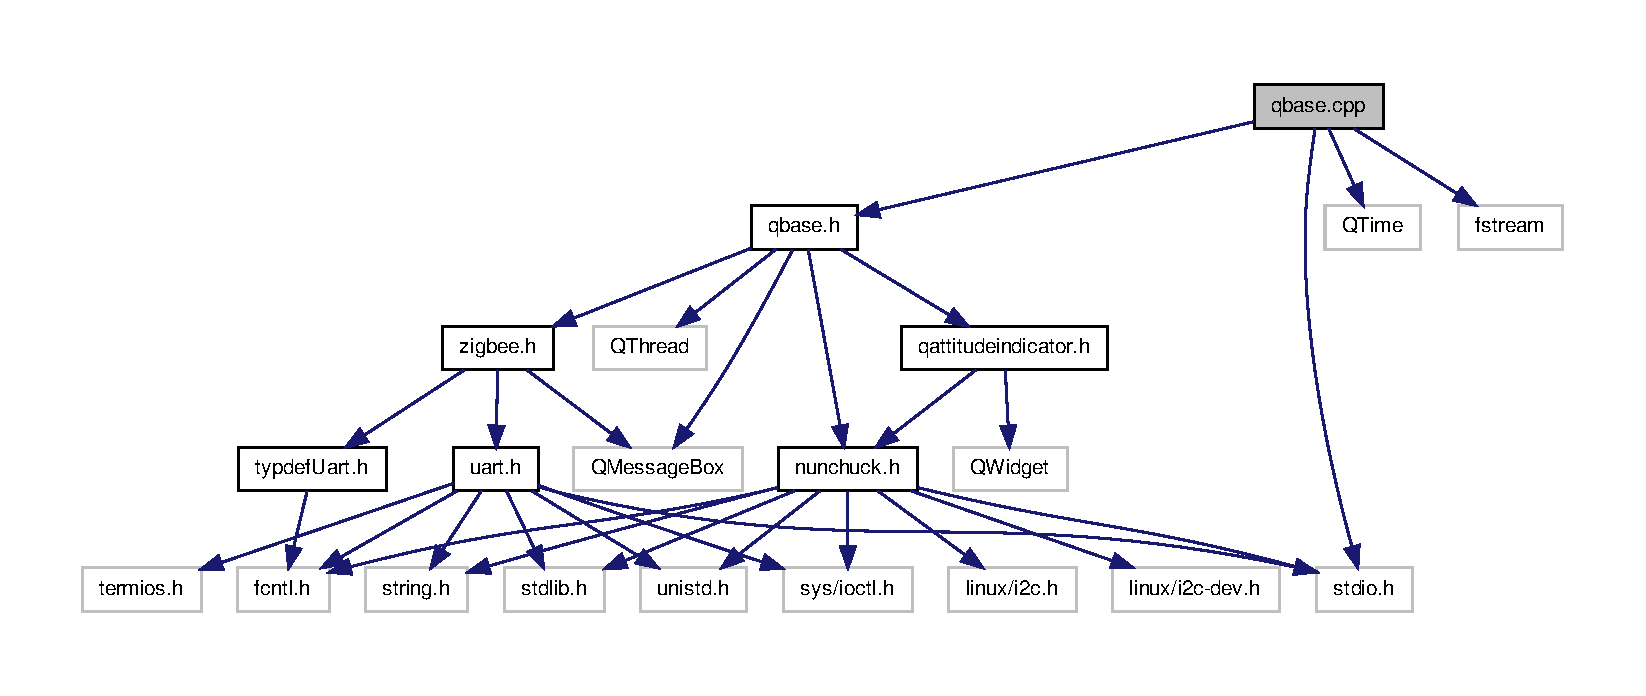
\includegraphics[width=350pt]{qbase_8cpp__incl}
\end{center}
\end{figure}

\hypertarget{qbase_8h}{\section{qbase.\-h File Reference}
\label{qbase_8h}\index{qbase.\-h@{qbase.\-h}}
}
{\ttfamily \#include $<$Q\-Thread$>$}\\*
{\ttfamily \#include $<$Q\-Message\-Box$>$}\\*
{\ttfamily \#include \char`\"{}nunchuck.\-h\char`\"{}}\\*
{\ttfamily \#include \char`\"{}zigbee.\-h\char`\"{}}\\*
{\ttfamily \#include \char`\"{}qattitudeindicator.\-h\char`\"{}}\\*
Include dependency graph for qbase.\-h\-:\nopagebreak
\begin{figure}[H]
\begin{center}
\leavevmode
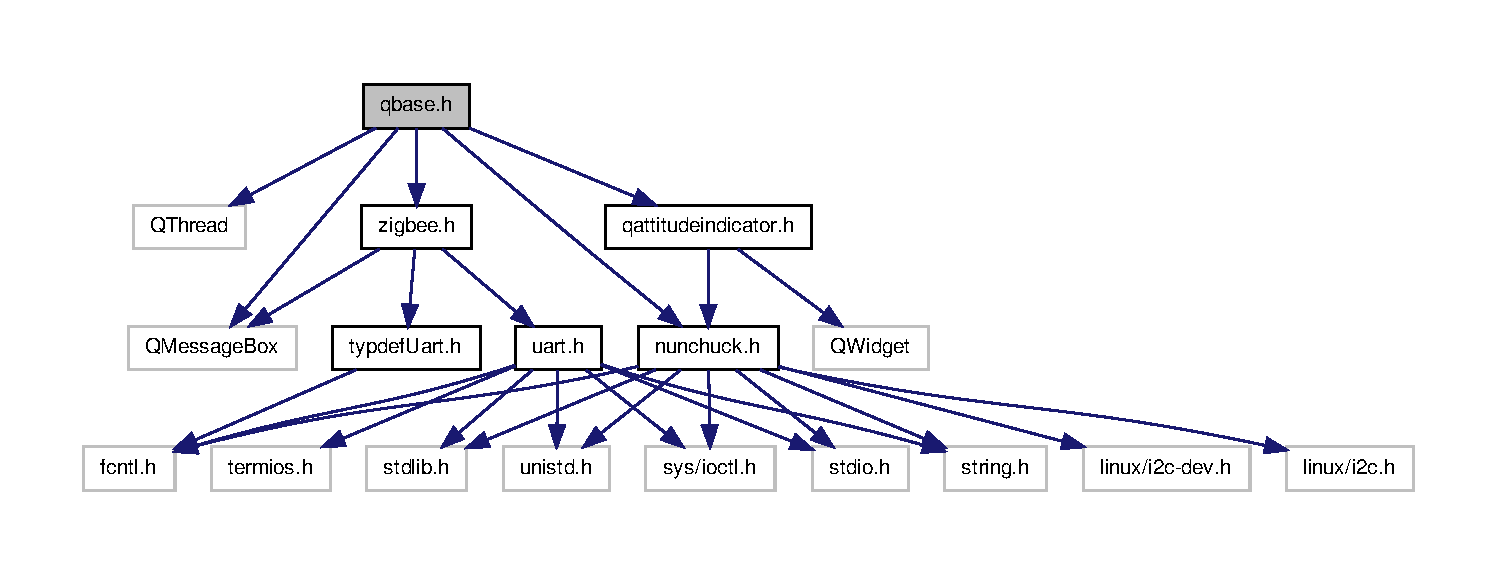
\includegraphics[width=350pt]{qbase_8h__incl}
\end{center}
\end{figure}
This graph shows which files directly or indirectly include this file\-:\nopagebreak
\begin{figure}[H]
\begin{center}
\leavevmode
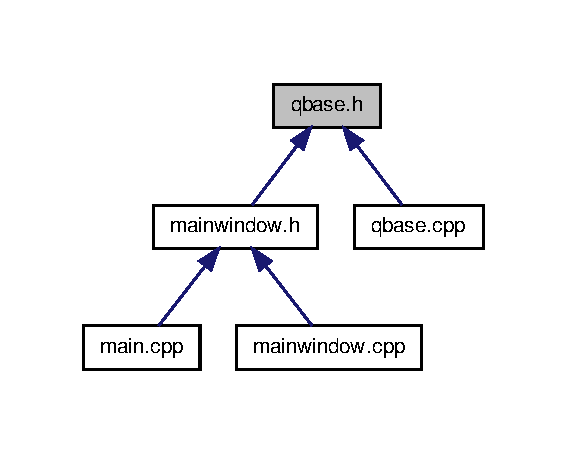
\includegraphics[width=272pt]{qbase_8h__dep__incl}
\end{center}
\end{figure}
\subsection*{Classes}
\begin{DoxyCompactItemize}
\item 
class \hyperlink{classQBase}{Q\-Base}
\end{DoxyCompactItemize}

\hypertarget{qth__base_8cpp}{\section{qth\-\_\-base.\-cpp File Reference}
\label{qth__base_8cpp}\index{qth\-\_\-base.\-cpp@{qth\-\_\-base.\-cpp}}
}
{\ttfamily \#include \char`\"{}qth\-\_\-base.\-h\char`\"{}}\\*
Include dependency graph for qth\-\_\-base.\-cpp\-:\nopagebreak
\begin{figure}[H]
\begin{center}
\leavevmode
\includegraphics[width=350pt]{qth__base_8cpp__incl}
\end{center}
\end{figure}

\hypertarget{qth__base_8h}{\section{qth\-\_\-base.\-h File Reference}
\label{qth__base_8h}\index{qth\-\_\-base.\-h@{qth\-\_\-base.\-h}}
}
{\ttfamily \#include $<$Q\-Thread$>$}\\*
{\ttfamily \#include \char`\"{}qattitudeindicator.\-h\char`\"{}}\\*
Include dependency graph for qth\-\_\-base.\-h\-:\nopagebreak
\begin{figure}[H]
\begin{center}
\leavevmode
\includegraphics[width=350pt]{qth__base_8h__incl}
\end{center}
\end{figure}
This graph shows which files directly or indirectly include this file\-:\nopagebreak
\begin{figure}[H]
\begin{center}
\leavevmode
\includegraphics[width=154pt]{qth__base_8h__dep__incl}
\end{center}
\end{figure}
\subsection*{Classes}
\begin{DoxyCompactItemize}
\item 
class \hyperlink{classQTh__Base}{Q\-Th\-\_\-\-Base}
\end{DoxyCompactItemize}
\subsection*{Macros}
\begin{DoxyCompactItemize}
\item 
\#define \hyperlink{qth__base_8h_a2f3670a7586687feccfde021b896c2b8}{Q\-T\-H\-R\-E\-A\-D\-\_\-\-H\-O\-R\-I\-Z\-O\-N}~0
\item 
\#define \hyperlink{qth__base_8h_a252b70ead8dbf51b155ecb9f0c7fd15a}{Q\-T\-H\-R\-E\-A\-D\-\_\-\-C\-O\-M\-U\-N\-I\-C\-A\-T\-I\-O\-N}~1
\end{DoxyCompactItemize}


\subsection{Macro Definition Documentation}
\hypertarget{qth__base_8h_a252b70ead8dbf51b155ecb9f0c7fd15a}{\index{qth\-\_\-base.\-h@{qth\-\_\-base.\-h}!Q\-T\-H\-R\-E\-A\-D\-\_\-\-C\-O\-M\-U\-N\-I\-C\-A\-T\-I\-O\-N@{Q\-T\-H\-R\-E\-A\-D\-\_\-\-C\-O\-M\-U\-N\-I\-C\-A\-T\-I\-O\-N}}
\index{Q\-T\-H\-R\-E\-A\-D\-\_\-\-C\-O\-M\-U\-N\-I\-C\-A\-T\-I\-O\-N@{Q\-T\-H\-R\-E\-A\-D\-\_\-\-C\-O\-M\-U\-N\-I\-C\-A\-T\-I\-O\-N}!qth_base.h@{qth\-\_\-base.\-h}}
\subsubsection[{Q\-T\-H\-R\-E\-A\-D\-\_\-\-C\-O\-M\-U\-N\-I\-C\-A\-T\-I\-O\-N}]{\setlength{\rightskip}{0pt plus 5cm}\#define Q\-T\-H\-R\-E\-A\-D\-\_\-\-C\-O\-M\-U\-N\-I\-C\-A\-T\-I\-O\-N~1}}\label{qth__base_8h_a252b70ead8dbf51b155ecb9f0c7fd15a}


Definition at line 8 of file qth\-\_\-base.\-h.

\hypertarget{qth__base_8h_a2f3670a7586687feccfde021b896c2b8}{\index{qth\-\_\-base.\-h@{qth\-\_\-base.\-h}!Q\-T\-H\-R\-E\-A\-D\-\_\-\-H\-O\-R\-I\-Z\-O\-N@{Q\-T\-H\-R\-E\-A\-D\-\_\-\-H\-O\-R\-I\-Z\-O\-N}}
\index{Q\-T\-H\-R\-E\-A\-D\-\_\-\-H\-O\-R\-I\-Z\-O\-N@{Q\-T\-H\-R\-E\-A\-D\-\_\-\-H\-O\-R\-I\-Z\-O\-N}!qth_base.h@{qth\-\_\-base.\-h}}
\subsubsection[{Q\-T\-H\-R\-E\-A\-D\-\_\-\-H\-O\-R\-I\-Z\-O\-N}]{\setlength{\rightskip}{0pt plus 5cm}\#define Q\-T\-H\-R\-E\-A\-D\-\_\-\-H\-O\-R\-I\-Z\-O\-N~0}}\label{qth__base_8h_a2f3670a7586687feccfde021b896c2b8}


Definition at line 7 of file qth\-\_\-base.\-h.



Referenced by Q\-Th\-\_\-\-Base\-::\-Q\-Th\-\_\-\-Base(), and Q\-Th\-\_\-\-Base\-::run().


\hypertarget{slippymap_8cpp}{\section{slippymap.\-cpp File Reference}
\label{slippymap_8cpp}\index{slippymap.\-cpp@{slippymap.\-cpp}}
}
{\ttfamily \#include $<$math.\-h$>$}\\*
{\ttfamily \#include $<$Qt\-Gui$>$}\\*
{\ttfamily \#include $<$Qt\-Network$>$}\\*
{\ttfamily \#include \char`\"{}slippymap.\-h\char`\"{}}\\*
Include dependency graph for slippymap.\-cpp\-:\nopagebreak
\begin{figure}[H]
\begin{center}
\leavevmode
\includegraphics[width=350pt]{slippymap_8cpp__incl}
\end{center}
\end{figure}
\subsection*{Macros}
\begin{DoxyCompactItemize}
\item 
\#define \hyperlink{slippymap_8cpp_ae71449b1cc6e6250b91f539153a7a0d3}{M\-\_\-\-P\-I}~3.\-14159265358979323846
\end{DoxyCompactItemize}
\subsection*{Functions}
\begin{DoxyCompactItemize}
\item 
uint \hyperlink{slippymap_8cpp_acc2ff595306dab2c33e934d7e24edac3}{q\-Hash} (const Q\-Point \&p)
\item 
Q\-Point\-F \hyperlink{slippymap_8cpp_a7b006b28fd0e4ace99c58e6162b501c9}{tile\-For\-Coordinate} (qreal lat, qreal lng, int zoom)
\item 
qreal \hyperlink{slippymap_8cpp_abfafaf71741cb91b95caa7218bf2993e}{longitude\-From\-Tile} (qreal tx, int zoom)
\item 
qreal \hyperlink{slippymap_8cpp_adbe934a4ade6aa7f2e0d82a4fe6e71e3}{latitude\-From\-Tile} (qreal ty, int zoom)
\end{DoxyCompactItemize}
\subsection*{Variables}
\begin{DoxyCompactItemize}
\item 
const int \hyperlink{slippymap_8cpp_a8ce10e914ae6c794640aeae2e2781d83}{tdim} = 256
\end{DoxyCompactItemize}


\subsection{Macro Definition Documentation}
\hypertarget{slippymap_8cpp_ae71449b1cc6e6250b91f539153a7a0d3}{\index{slippymap.\-cpp@{slippymap.\-cpp}!M\-\_\-\-P\-I@{M\-\_\-\-P\-I}}
\index{M\-\_\-\-P\-I@{M\-\_\-\-P\-I}!slippymap.cpp@{slippymap.\-cpp}}
\subsubsection[{M\-\_\-\-P\-I}]{\setlength{\rightskip}{0pt plus 5cm}\#define M\-\_\-\-P\-I~3.\-14159265358979323846}}\label{slippymap_8cpp_ae71449b1cc6e6250b91f539153a7a0d3}


Definition at line 7 of file slippymap.\-cpp.



Referenced by latitude\-From\-Tile(), and tile\-For\-Coordinate().



\subsection{Function Documentation}
\hypertarget{slippymap_8cpp_adbe934a4ade6aa7f2e0d82a4fe6e71e3}{\index{slippymap.\-cpp@{slippymap.\-cpp}!latitude\-From\-Tile@{latitude\-From\-Tile}}
\index{latitude\-From\-Tile@{latitude\-From\-Tile}!slippymap.cpp@{slippymap.\-cpp}}
\subsubsection[{latitude\-From\-Tile}]{\setlength{\rightskip}{0pt plus 5cm}qreal latitude\-From\-Tile (
\begin{DoxyParamCaption}
\item[{qreal}]{ty, }
\item[{int}]{zoom}
\end{DoxyParamCaption}
)}}\label{slippymap_8cpp_adbe934a4ade6aa7f2e0d82a4fe6e71e3}


Definition at line 34 of file slippymap.\-cpp.



References M\-\_\-\-P\-I.



Referenced by Slippy\-Map\-::pan().


\begin{DoxyCode}
\{
    qreal zn = \textcolor{keyword}{static\_cast<}qreal\textcolor{keyword}{>}(1 << zoom);
    qreal n = \hyperlink{slippymap_8cpp_ae71449b1cc6e6250b91f539153a7a0d3}{M\_PI} - 2 * \hyperlink{slippymap_8cpp_ae71449b1cc6e6250b91f539153a7a0d3}{M\_PI} * ty / zn;
    qreal lng = 180.0 / \hyperlink{slippymap_8cpp_ae71449b1cc6e6250b91f539153a7a0d3}{M\_PI} * atan(0.5 * (exp(n) - exp(-n)));
    \textcolor{keywordflow}{return} lng;
\}
\end{DoxyCode}
\hypertarget{slippymap_8cpp_abfafaf71741cb91b95caa7218bf2993e}{\index{slippymap.\-cpp@{slippymap.\-cpp}!longitude\-From\-Tile@{longitude\-From\-Tile}}
\index{longitude\-From\-Tile@{longitude\-From\-Tile}!slippymap.cpp@{slippymap.\-cpp}}
\subsubsection[{longitude\-From\-Tile}]{\setlength{\rightskip}{0pt plus 5cm}qreal longitude\-From\-Tile (
\begin{DoxyParamCaption}
\item[{qreal}]{tx, }
\item[{int}]{zoom}
\end{DoxyParamCaption}
)}}\label{slippymap_8cpp_abfafaf71741cb91b95caa7218bf2993e}


Definition at line 27 of file slippymap.\-cpp.



Referenced by Slippy\-Map\-::pan().


\begin{DoxyCode}
\{
    qreal zn = \textcolor{keyword}{static\_cast<}qreal\textcolor{keyword}{>}(1 << zoom);
    qreal lat = tx / zn * 360.0 - 180.0;
    \textcolor{keywordflow}{return} lat;
\}
\end{DoxyCode}
\hypertarget{slippymap_8cpp_acc2ff595306dab2c33e934d7e24edac3}{\index{slippymap.\-cpp@{slippymap.\-cpp}!q\-Hash@{q\-Hash}}
\index{q\-Hash@{q\-Hash}!slippymap.cpp@{slippymap.\-cpp}}
\subsubsection[{q\-Hash}]{\setlength{\rightskip}{0pt plus 5cm}uint q\-Hash (
\begin{DoxyParamCaption}
\item[{const Q\-Point \&}]{p}
\end{DoxyParamCaption}
)}}\label{slippymap_8cpp_acc2ff595306dab2c33e934d7e24edac3}


Definition at line 10 of file slippymap.\-cpp.


\begin{DoxyCode}
\{
    \textcolor{keywordflow}{return} p.x() * 17 ^ p.y();
\}
\end{DoxyCode}
\hypertarget{slippymap_8cpp_a7b006b28fd0e4ace99c58e6162b501c9}{\index{slippymap.\-cpp@{slippymap.\-cpp}!tile\-For\-Coordinate@{tile\-For\-Coordinate}}
\index{tile\-For\-Coordinate@{tile\-For\-Coordinate}!slippymap.cpp@{slippymap.\-cpp}}
\subsubsection[{tile\-For\-Coordinate}]{\setlength{\rightskip}{0pt plus 5cm}Q\-Point\-F tile\-For\-Coordinate (
\begin{DoxyParamCaption}
\item[{qreal}]{lat, }
\item[{qreal}]{lng, }
\item[{int}]{zoom}
\end{DoxyParamCaption}
)}}\label{slippymap_8cpp_a7b006b28fd0e4ace99c58e6162b501c9}


Definition at line 18 of file slippymap.\-cpp.



References M\-\_\-\-P\-I.



Referenced by Slippy\-Map\-::invalidate(), Slippy\-Map\-::pan(), and Slippy\-Map\-::render().


\begin{DoxyCode}
\{
    qreal zn = \textcolor{keyword}{static\_cast<}qreal\textcolor{keyword}{>}(1 << zoom);
    qreal tx = (lng + 180.0) / 360.0;
    qreal ty = (1.0 - log(tan(lat * \hyperlink{slippymap_8cpp_ae71449b1cc6e6250b91f539153a7a0d3}{M\_PI} / 180.0) +
                          1.0 / cos(lat * \hyperlink{slippymap_8cpp_ae71449b1cc6e6250b91f539153a7a0d3}{M\_PI} / 180.0)) / \hyperlink{slippymap_8cpp_ae71449b1cc6e6250b91f539153a7a0d3}{M\_PI}) / 2.0;
    \textcolor{keywordflow}{return} QPointF(tx * zn, ty * zn);
\}
\end{DoxyCode}


\subsection{Variable Documentation}
\hypertarget{slippymap_8cpp_a8ce10e914ae6c794640aeae2e2781d83}{\index{slippymap.\-cpp@{slippymap.\-cpp}!tdim@{tdim}}
\index{tdim@{tdim}!slippymap.cpp@{slippymap.\-cpp}}
\subsubsection[{tdim}]{\setlength{\rightskip}{0pt plus 5cm}const int tdim = 256}}\label{slippymap_8cpp_a8ce10e914ae6c794640aeae2e2781d83}


Definition at line 16 of file slippymap.\-cpp.



Referenced by Slippy\-Map\-::invalidate(), Slippy\-Map\-::pan(), Slippy\-Map\-::\-Slippy\-Map(), and Slippy\-Map\-::tile\-Rect().


\hypertarget{slippymap_8h}{\section{slippymap.\-h File Reference}
\label{slippymap_8h}\index{slippymap.\-h@{slippymap.\-h}}
}
{\ttfamily \#include $<$Qt\-Network$>$}\\*
{\ttfamily \#include $<$Q\-Pixmap$>$}\\*
{\ttfamily \#include $<$Q\-Url$>$}\\*
Include dependency graph for slippymap.\-h\-:\nopagebreak
\begin{figure}[H]
\begin{center}
\leavevmode
\includegraphics[width=272pt]{slippymap_8h__incl}
\end{center}
\end{figure}
This graph shows which files directly or indirectly include this file\-:\nopagebreak
\begin{figure}[H]
\begin{center}
\leavevmode
\includegraphics[width=350pt]{slippymap_8h__dep__incl}
\end{center}
\end{figure}
\subsection*{Classes}
\begin{DoxyCompactItemize}
\item 
class \hyperlink{classSlippyMap}{Slippy\-Map}
\end{DoxyCompactItemize}

\hypertarget{typdefUart_8h}{\section{typdef\-Uart.\-h File Reference}
\label{typdefUart_8h}\index{typdef\-Uart.\-h@{typdef\-Uart.\-h}}
}
{\ttfamily \#include $<$fcntl.\-h$>$}\\*
Include dependency graph for typdef\-Uart.\-h\-:\nopagebreak
\begin{figure}[H]
\begin{center}
\leavevmode
\includegraphics[width=150pt]{typdefUart_8h__incl}
\end{center}
\end{figure}
This graph shows which files directly or indirectly include this file\-:\nopagebreak
\begin{figure}[H]
\begin{center}
\leavevmode
\includegraphics[width=304pt]{typdefUart_8h__dep__incl}
\end{center}
\end{figure}
\subsection*{Classes}
\begin{DoxyCompactItemize}
\item 
struct \hyperlink{structtramZigbee}{tram\-Zigbee}
\item 
struct \hyperlink{structdroneConfig}{drone\-Config}
\item 
struct \hyperlink{structflightCommand}{flight\-Command}
\item 
struct \hyperlink{structdroneState}{drone\-State}
\item 
struct \hyperlink{structdroneIMUData}{drone\-I\-M\-U\-Data}
\item 
struct \hyperlink{structdroneGPSData}{drone\-G\-P\-S\-Data}
\item 
struct \hyperlink{structdroneTelemeterData}{drone\-Telemeter\-Data}
\item 
struct \hyperlink{structdroneBatteryData}{drone\-Battery\-Data}
\end{DoxyCompactItemize}
\subsection*{Typedefs}
\begin{DoxyCompactItemize}
\item 
typedef unsigned int \hyperlink{typdefUart_8h_a435d1572bf3f880d55459d9805097f62}{uint32\-\_\-t}
\item 
typedef \hyperlink{typdefUart_8h_a435d1572bf3f880d55459d9805097f62}{uint32\-\_\-t} \hyperlink{typdefUart_8h_ae9fa5e001303f1be1c0294f26cde8caf}{port\-Tick\-Type}
\item 
typedef unsigned char \hyperlink{typdefUart_8h_aba7bc1797add20fe3efdf37ced1182c5}{uint8\-\_\-t}
\end{DoxyCompactItemize}
\subsection*{Enumerations}
\begin{DoxyCompactItemize}
\item 
enum \hyperlink{typdefUart_8h_aa8a212aca1d1f49ff85fe2ac4b74cbb6}{zigbee\-Command\-Id} \{ \\*
\hyperlink{typdefUart_8h_aa8a212aca1d1f49ff85fe2ac4b74cbb6a239722b6c1371469bb65b83c5aa92a31}{C\-M\-D\-\_\-\-R\-E\-B\-O\-O\-T}, 
\hyperlink{typdefUart_8h_aa8a212aca1d1f49ff85fe2ac4b74cbb6a8bbf29869938b9b99e9e98e2685c2af0}{C\-M\-D\-\_\-\-S\-H\-U\-T\-D\-O\-W\-N}, 
\hyperlink{typdefUart_8h_aa8a212aca1d1f49ff85fe2ac4b74cbb6abb5a621b2e8f98474199365307c1583c}{C\-M\-D\-\_\-\-V\-I\-D\-E\-O\-\_\-\-E\-N\-A\-B\-L\-E}, 
\hyperlink{typdefUart_8h_aa8a212aca1d1f49ff85fe2ac4b74cbb6a3147545d7cf162c55a4dfdb8a9b842f8}{C\-M\-D\-\_\-\-V\-I\-D\-E\-O\-\_\-\-D\-I\-S\-A\-B\-L\-E}, 
\\*
\hyperlink{typdefUart_8h_aa8a212aca1d1f49ff85fe2ac4b74cbb6a4c63207daec4bc4c947f0a63d48761cb}{C\-M\-D\-\_\-\-F\-L\-T\-\_\-\-T\-A\-K\-E\-O\-F\-F}, 
\hyperlink{typdefUart_8h_aa8a212aca1d1f49ff85fe2ac4b74cbb6a7f3b918346242aa7d684a14ba2c2b441}{C\-M\-D\-\_\-\-F\-L\-T\-\_\-\-L\-A\-N\-D\-I\-N\-G}, 
\hyperlink{typdefUart_8h_aa8a212aca1d1f49ff85fe2ac4b74cbb6ae0ea43f407f8211a9acef5f717dcf933}{C\-M\-D\-\_\-\-F\-L\-T\-\_\-\-A\-U\-T\-O\-T\-U\-N\-I\-N\-G}, 
\hyperlink{typdefUart_8h_aa8a212aca1d1f49ff85fe2ac4b74cbb6a79510fc7f07b52c1fef87c672e3a9d9e}{C\-M\-D\-\_\-\-R\-E\-S\-E\-T\-\_\-\-A\-U\-T\-O\-T\-U\-N\-I\-N\-G}, 
\\*
\hyperlink{typdefUart_8h_aa8a212aca1d1f49ff85fe2ac4b74cbb6a77553c4f9197b5892c5827a04c25a968}{C\-M\-D\-\_\-\-S\-E\-T\-\_\-\-C\-O\-N\-F\-I\-G}, 
\hyperlink{typdefUart_8h_aa8a212aca1d1f49ff85fe2ac4b74cbb6a824277770f43b1df4f00e8ee24b1d26c}{C\-M\-D\-\_\-\-R\-E\-S\-E\-T\-\_\-\-C\-O\-N\-F\-I\-G}, 
\hyperlink{typdefUart_8h_aa8a212aca1d1f49ff85fe2ac4b74cbb6a72722dc0846a5fc226f850301b703609}{C\-M\-D\-\_\-\-G\-E\-T\-\_\-\-C\-O\-N\-F\-I\-G}, 
\hyperlink{typdefUart_8h_aa8a212aca1d1f49ff85fe2ac4b74cbb6aa9f5e1d3fa7a48a053cb78acdf95e57a}{C\-M\-D\-\_\-\-G\-E\-T\-\_\-\-S\-T\-A\-T\-U\-S}, 
\\*
\hyperlink{typdefUart_8h_aa8a212aca1d1f49ff85fe2ac4b74cbb6aefb30be8a8f1fedd95be57cd09c85398}{C\-M\-D\-\_\-\-F\-L\-T\-\_\-\-M\-A\-N\-E\-U\-V\-E\-R}, 
\hyperlink{typdefUart_8h_aa8a212aca1d1f49ff85fe2ac4b74cbb6a7b05a94faeba01c6ca01fc3f46b740af}{C\-M\-D\-\_\-\-E\-R\-R\-\_\-\-I\-G\-N\-O\-R\-E}
 \}
\item 
enum \hyperlink{typdefUart_8h_a7fdf1e7bfbebe0c7a2eb84a10e069632}{tram\-Data\-Id} \{ \\*
\hyperlink{typdefUart_8h_a7fdf1e7bfbebe0c7a2eb84a10e069632a7828400a62571bb441a0216f1c2e29be}{P\-A\-R\-A\-M\-\_\-\-D\-R\-O\-N\-E\-\_\-\-C\-O\-N\-F\-I\-G\-\_\-ul\-Max\-Angle}, 
\hyperlink{typdefUart_8h_a7fdf1e7bfbebe0c7a2eb84a10e069632af954ea9792a880b2593da24e0214708f}{P\-A\-R\-A\-M\-\_\-\-D\-R\-O\-N\-E\-\_\-\-C\-O\-N\-F\-I\-G\-\_\-ul\-Takeoff\-Altitude}, 
\hyperlink{typdefUart_8h_a7fdf1e7bfbebe0c7a2eb84a10e069632a516ded0a007275ce22b40cba97734484}{P\-A\-R\-A\-M\-\_\-\-D\-R\-O\-N\-E\-\_\-\-C\-O\-N\-F\-I\-G\-\_\-ul\-Min\-Altitude}, 
\hyperlink{typdefUart_8h_a7fdf1e7bfbebe0c7a2eb84a10e069632a212c640074147bd9d0d63888d538d256}{P\-A\-R\-A\-M\-\_\-\-D\-R\-O\-N\-E\-\_\-\-C\-O\-N\-F\-I\-G\-\_\-ul\-Crit\-Battery\-Lvl}, 
\\*
\hyperlink{typdefUart_8h_a7fdf1e7bfbebe0c7a2eb84a10e069632adc16eed85f98b926f829decb1e7f3175}{P\-A\-R\-A\-M\-\_\-\-D\-R\-O\-N\-E\-\_\-\-C\-O\-N\-F\-I\-G\-\_\-ul\-Crit\-Obstacle\-Dist}, 
\hyperlink{typdefUart_8h_a7fdf1e7bfbebe0c7a2eb84a10e069632a91adcfa9ba7373cb5e94cb7dad749286}{P\-A\-R\-A\-M\-\_\-\-D\-R\-O\-N\-E\-\_\-\-C\-O\-N\-F\-I\-G\-\_\-ul\-Crit\-Zigbee\-Signal\-Lvl}, 
\hyperlink{typdefUart_8h_a7fdf1e7bfbebe0c7a2eb84a10e069632adaafa83d8768d26374d1cca8f3c4914d}{P\-A\-R\-A\-M\-\_\-\-D\-R\-O\-N\-E\-\_\-\-C\-O\-N\-F\-I\-G\-\_\-x\-Battery\-Monitoring\-Period}, 
\hyperlink{typdefUart_8h_a7fdf1e7bfbebe0c7a2eb84a10e069632a70d207333012bb820cb3576f3fad9048}{P\-A\-R\-A\-M\-\_\-\-D\-R\-O\-N\-E\-\_\-\-C\-O\-N\-F\-I\-G\-\_\-x\-Detect\-Obstacle\-Period}, 
\\*
\hyperlink{typdefUart_8h_a7fdf1e7bfbebe0c7a2eb84a10e069632a5c305ec532822ca3aa2ff74d0052f757}{P\-A\-R\-A\-M\-\_\-\-D\-R\-O\-N\-E\-\_\-\-C\-O\-N\-F\-I\-G\-\_\-x\-Zigbee\-Receive\-Period}, 
\hyperlink{typdefUart_8h_a7fdf1e7bfbebe0c7a2eb84a10e069632a22871458b110498e27a8b6244d14fd4e}{P\-A\-R\-A\-M\-\_\-\-D\-R\-O\-N\-E\-\_\-\-C\-O\-N\-F\-I\-G\-\_\-x\-Flight\-Ctrl\-Period}, 
\hyperlink{typdefUart_8h_a7fdf1e7bfbebe0c7a2eb84a10e069632a80df4e54f488c528a0af260bf4287bcb}{P\-A\-R\-A\-M\-\_\-\-D\-R\-O\-N\-E\-\_\-\-C\-O\-N\-F\-I\-G\-\_\-x\-G\-P\-S\-Receive\-Period}, 
\hyperlink{typdefUart_8h_a7fdf1e7bfbebe0c7a2eb84a10e069632a590b78e1b29c0c8dcdf6d2dc869e43aa}{P\-A\-R\-A\-M\-\_\-\-D\-R\-O\-N\-E\-\_\-\-C\-O\-N\-F\-I\-G\-\_\-x\-Video\-Toggle\-Period}, 
\\*
\hyperlink{typdefUart_8h_a7fdf1e7bfbebe0c7a2eb84a10e069632a8bd205ac7401d53092ff7ffc98e754aa}{P\-A\-R\-A\-M\-\_\-\-D\-R\-O\-N\-E\-\_\-\-C\-O\-N\-F\-I\-G\-\_\-x\-I\-M\-U\-Data\-Timeout}, 
\hyperlink{typdefUart_8h_a7fdf1e7bfbebe0c7a2eb84a10e069632afaa7777e435be6b471009c6cdf74c948}{P\-A\-R\-A\-M\-\_\-\-D\-R\-O\-N\-E\-\_\-\-C\-O\-N\-F\-I\-G\-\_\-x\-Zigbee\-Cmd\-Timeout}, 
\hyperlink{typdefUart_8h_a7fdf1e7bfbebe0c7a2eb84a10e069632af2f4da476de6fc43e2118826e9e8bc9b}{P\-A\-R\-A\-M\-\_\-\-D\-R\-O\-N\-E\-\_\-\-C\-O\-N\-F\-I\-G\-\_\-x\-Zigbee\-Receive\-Timeout}, 
\hyperlink{typdefUart_8h_a7fdf1e7bfbebe0c7a2eb84a10e069632aa01da571181efda4755ff66c627d007e}{P\-A\-R\-A\-M\-\_\-\-D\-R\-O\-N\-E\-\_\-\-C\-O\-N\-F\-I\-G\-\_\-x\-Telemeter\-Timeout}, 
\\*
\hyperlink{typdefUart_8h_a7fdf1e7bfbebe0c7a2eb84a10e069632a1298f95dd257a888bde3262a86c4d136}{P\-A\-R\-A\-M\-\_\-\-D\-R\-O\-N\-E\-\_\-\-C\-O\-N\-F\-I\-G\-\_\-x\-Battery\-Timeout}, 
\hyperlink{typdefUart_8h_a7fdf1e7bfbebe0c7a2eb84a10e069632a9cd65980217626ee680a9055e78d4131}{P\-A\-R\-A\-M\-\_\-\-D\-R\-O\-N\-E\-\_\-\-C\-O\-N\-F\-I\-G\-\_\-x\-G\-P\-S\-Timeout}, 
\hyperlink{typdefUart_8h_a7fdf1e7bfbebe0c7a2eb84a10e069632a653f0737cc2f062b0f5563ee5c9023e4}{P\-A\-R\-A\-M\-\_\-\-C\-M\-D\-\_\-\-I\-D}, 
\hyperlink{typdefUart_8h_a7fdf1e7bfbebe0c7a2eb84a10e069632ab52e565f8ee0b43ab5fdba5dd32ef949}{P\-A\-R\-A\-M\-\_\-\-C\-M\-D\-\_\-\-D\-R\-O\-N\-E}, 
\\*
\hyperlink{typdefUart_8h_a7fdf1e7bfbebe0c7a2eb84a10e069632a8f2ad857311b305a40e6294736196f47}{P\-A\-R\-A\-M\-\_\-\-F\-L\-Y\-\_\-\-S\-T\-A\-T\-E}, 
\hyperlink{typdefUart_8h_a7fdf1e7bfbebe0c7a2eb84a10e069632a01acce445241211e5ef11328c1b8d1e2}{P\-A\-R\-A\-M\-\_\-\-D\-R\-O\-N\-E\-\_\-\-E\-R\-R\-O\-R}, 
\hyperlink{typdefUart_8h_a7fdf1e7bfbebe0c7a2eb84a10e069632aba9ba51d13875fc28dbcb7aefb4706b2}{P\-A\-R\-A\-M\-\_\-\-I\-M\-U\-\_\-x\-Update\-Time}, 
\hyperlink{typdefUart_8h_a7fdf1e7bfbebe0c7a2eb84a10e069632af3fc4126f4c3a7540f615932cf7b6144}{P\-A\-R\-A\-M\-\_\-\-G\-P\-S\-\_\-x\-Update\-Time}, 
\\*
\hyperlink{typdefUart_8h_a7fdf1e7bfbebe0c7a2eb84a10e069632a5b5200507842f7d81676e1fc196b9a03}{P\-A\-R\-A\-M\-\_\-\-T\-E\-L\-M\-\_\-x\-Update\-Time}, 
\hyperlink{typdefUart_8h_a7fdf1e7bfbebe0c7a2eb84a10e069632a84d1fa4a6fe3f1b379971515cbab995d}{P\-A\-R\-A\-M\-\_\-\-B\-A\-T\-\_\-ul\-Power\-Lvl}, 
\hyperlink{typdefUart_8h_a7fdf1e7bfbebe0c7a2eb84a10e069632aa12b8c52c4643e91d235de4613b56ee1}{P\-A\-R\-A\-M\-\_\-\-B\-A\-T\-\_\-x\-Update\-Time}
 \}
\item 
enum \hyperlink{typdefUart_8h_aac9034800b5ef8e755ade03d164e3b6c}{drone\-Flt\-State} \{ \\*
\hyperlink{typdefUart_8h_aac9034800b5ef8e755ade03d164e3b6caa5f51c4eb8c8eec3b16b058c5e29a037}{S\-T\-A\-T\-E\-\_\-\-S\-T\-A\-R\-T\-I\-N\-G}, 
\hyperlink{typdefUart_8h_aac9034800b5ef8e755ade03d164e3b6ca6bbc8323e31abccea998c00dfe5d20a0}{S\-T\-A\-T\-E\-\_\-\-G\-R\-O\-U\-N\-D\-\_\-\-R\-D\-Y}, 
\hyperlink{typdefUart_8h_aac9034800b5ef8e755ade03d164e3b6ca0cab358e8f859a193657d1d9b854c235}{S\-T\-A\-T\-E\-\_\-\-G\-R\-O\-U\-N\-D\-\_\-\-E\-R\-R}, 
\hyperlink{typdefUart_8h_aac9034800b5ef8e755ade03d164e3b6ca53e82bf3cade7e163576fa495996d853}{S\-T\-A\-T\-E\-\_\-\-T\-A\-K\-E\-O\-F\-F}, 
\\*
\hyperlink{typdefUart_8h_aac9034800b5ef8e755ade03d164e3b6cadaf68b8f3e3aa6f6f7250e8965aa720c}{S\-T\-A\-T\-E\-\_\-\-F\-L\-I\-G\-H\-T}, 
\hyperlink{typdefUart_8h_aac9034800b5ef8e755ade03d164e3b6cad4e643150006cdb1e80a11aa25cd860f}{S\-T\-A\-T\-E\-\_\-\-A\-U\-T\-O\-T\-U\-N\-I\-N\-G}, 
\hyperlink{typdefUart_8h_aac9034800b5ef8e755ade03d164e3b6caed26b59c0afa78ad7080428ba383e2fa}{S\-T\-A\-T\-E\-\_\-\-F\-L\-I\-G\-H\-T\-\_\-\-E\-R\-R}, 
\hyperlink{typdefUart_8h_aac9034800b5ef8e755ade03d164e3b6ca8022b6b06eea757154be17d06c5441b7}{S\-T\-A\-T\-E\-\_\-\-L\-A\-N\-D\-I\-N\-G}
 \}
\item 
enum \hyperlink{typdefUart_8h_aad4124e5a34e185d704fe88506ecf352}{drone\-Error} \{ \\*
\hyperlink{typdefUart_8h_aad4124e5a34e185d704fe88506ecf352a4eb8e22beceecc6e83a76fc46f56e03a}{D\-R\-N\-\_\-\-E\-R\-R\-\_\-\-N\-O\-N\-E} =  0x00, 
\hyperlink{typdefUart_8h_aad4124e5a34e185d704fe88506ecf352a6490e84f47f8baed82eb8ec0c3635ee5}{D\-R\-N\-\_\-\-E\-R\-R\-\_\-\-T\-L\-M\-\_\-\-T\-O\-U\-T} =  0x01, 
\hyperlink{typdefUart_8h_aad4124e5a34e185d704fe88506ecf352a475a89ae9e8123cb50bbcd0fd519dd66}{D\-R\-N\-\_\-\-E\-R\-R\-\_\-\-T\-L\-M\-\_\-\-I\-N\-V\-A\-L} =  0x02, 
\hyperlink{typdefUart_8h_aad4124e5a34e185d704fe88506ecf352a795b43a2f0a142565346125d00a27d60}{D\-R\-N\-\_\-\-E\-R\-R\-\_\-\-I\-M\-U\-\_\-\-T\-O\-U\-T} =  0x04, 
\\*
\hyperlink{typdefUart_8h_aad4124e5a34e185d704fe88506ecf352a65d6f68d28c3555056d18b2c273ac433}{D\-R\-N\-\_\-\-E\-R\-R\-\_\-\-I\-M\-U\-\_\-\-I\-N\-V\-A\-L} =  0x08, 
\hyperlink{typdefUart_8h_aad4124e5a34e185d704fe88506ecf352af0e3bb3a5358ffbf2efad0dbb7f6e45a}{D\-R\-N\-\_\-\-E\-R\-R\-\_\-\-G\-P\-S\-\_\-\-T\-O\-U\-T} =  0x10, 
\hyperlink{typdefUart_8h_aad4124e5a34e185d704fe88506ecf352a816cf76d244f3951ede4e2f8fb204af4}{D\-R\-N\-\_\-\-E\-R\-R\-\_\-\-G\-P\-S\-\_\-\-I\-N\-V\-A\-L} =  0x20, 
\hyperlink{typdefUart_8h_aad4124e5a34e185d704fe88506ecf352a4048ab78d8443f714af4f6cf9f5a1c0c}{D\-R\-N\-\_\-\-E\-R\-R\-\_\-\-C\-M\-D\-\_\-\-T\-O\-U\-T} =  0x40, 
\\*
\hyperlink{typdefUart_8h_aad4124e5a34e185d704fe88506ecf352ac6ac67da7d10405e907c3672d84b9186}{D\-R\-N\-\_\-\-E\-R\-R\-\_\-\-B\-A\-T\-T\-\_\-\-T\-O\-U\-T} =  0x80, 
\hyperlink{typdefUart_8h_aad4124e5a34e185d704fe88506ecf352a85117dc073a0b9e9143d5fc903512fb2}{D\-R\-N\-\_\-\-E\-R\-R\-\_\-\-B\-A\-T\-T\-\_\-\-I\-N\-V\-A\-L} =  0x100, 
\hyperlink{typdefUart_8h_aad4124e5a34e185d704fe88506ecf352a22848fed5eebff66eaeb5e262435ce77}{D\-R\-N\-\_\-\-E\-R\-R\-\_\-\-R\-X\-\_\-\-T\-O\-U\-T} =  0x200, 
\hyperlink{typdefUart_8h_aad4124e5a34e185d704fe88506ecf352a80138de1c3a91db00596e22a7544e0b2}{D\-R\-N\-\_\-\-E\-R\-R\-\_\-\-C\-O\-N\-F\-I\-G} =  0x400, 
\\*
\hyperlink{typdefUart_8h_aad4124e5a34e185d704fe88506ecf352ad87cede38525b6afdd6dc98bea304204}{D\-R\-N\-\_\-\-E\-R\-R\-\_\-\-C\-M\-D} =  0x800, 
\hyperlink{typdefUart_8h_aad4124e5a34e185d704fe88506ecf352a68060eb9b68ae5cd82c632ff11429c2f}{D\-R\-N\-\_\-\-E\-R\-R\-\_\-\-I\-N\-I\-T} =  0x8000
 \}
\end{DoxyCompactItemize}


\subsection{Typedef Documentation}
\hypertarget{typdefUart_8h_ae9fa5e001303f1be1c0294f26cde8caf}{\index{typdef\-Uart.\-h@{typdef\-Uart.\-h}!port\-Tick\-Type@{port\-Tick\-Type}}
\index{port\-Tick\-Type@{port\-Tick\-Type}!typdefUart.h@{typdef\-Uart.\-h}}
\subsubsection[{port\-Tick\-Type}]{\setlength{\rightskip}{0pt plus 5cm}typedef {\bf uint32\-\_\-t} {\bf port\-Tick\-Type}}}\label{typdefUart_8h_ae9fa5e001303f1be1c0294f26cde8caf}


Definition at line 10 of file typdef\-Uart.\-h.

\hypertarget{typdefUart_8h_a435d1572bf3f880d55459d9805097f62}{\index{typdef\-Uart.\-h@{typdef\-Uart.\-h}!uint32\-\_\-t@{uint32\-\_\-t}}
\index{uint32\-\_\-t@{uint32\-\_\-t}!typdefUart.h@{typdef\-Uart.\-h}}
\subsubsection[{uint32\-\_\-t}]{\setlength{\rightskip}{0pt plus 5cm}typedef unsigned int {\bf uint32\-\_\-t}}}\label{typdefUart_8h_a435d1572bf3f880d55459d9805097f62}


Definition at line 9 of file typdef\-Uart.\-h.

\hypertarget{typdefUart_8h_aba7bc1797add20fe3efdf37ced1182c5}{\index{typdef\-Uart.\-h@{typdef\-Uart.\-h}!uint8\-\_\-t@{uint8\-\_\-t}}
\index{uint8\-\_\-t@{uint8\-\_\-t}!typdefUart.h@{typdef\-Uart.\-h}}
\subsubsection[{uint8\-\_\-t}]{\setlength{\rightskip}{0pt plus 5cm}typedef unsigned char {\bf uint8\-\_\-t}}}\label{typdefUart_8h_aba7bc1797add20fe3efdf37ced1182c5}


Definition at line 12 of file typdef\-Uart.\-h.



\subsection{Enumeration Type Documentation}
\hypertarget{typdefUart_8h_aad4124e5a34e185d704fe88506ecf352}{\index{typdef\-Uart.\-h@{typdef\-Uart.\-h}!drone\-Error@{drone\-Error}}
\index{drone\-Error@{drone\-Error}!typdefUart.h@{typdef\-Uart.\-h}}
\subsubsection[{drone\-Error}]{\setlength{\rightskip}{0pt plus 5cm}enum {\bf drone\-Error}}}\label{typdefUart_8h_aad4124e5a34e185d704fe88506ecf352}
\begin{Desc}
\item[Enumerator\-: ]\par
\begin{description}
\index{D\-R\-N\-\_\-\-E\-R\-R\-\_\-\-N\-O\-N\-E@{D\-R\-N\-\_\-\-E\-R\-R\-\_\-\-N\-O\-N\-E}!typdef\-Uart.\-h@{typdef\-Uart.\-h}}\index{typdef\-Uart.\-h@{typdef\-Uart.\-h}!D\-R\-N\-\_\-\-E\-R\-R\-\_\-\-N\-O\-N\-E@{D\-R\-N\-\_\-\-E\-R\-R\-\_\-\-N\-O\-N\-E}}\item[{\em 
\hypertarget{typdefUart_8h_aad4124e5a34e185d704fe88506ecf352a4eb8e22beceecc6e83a76fc46f56e03a}{D\-R\-N\-\_\-\-E\-R\-R\-\_\-\-N\-O\-N\-E}\label{typdefUart_8h_aad4124e5a34e185d704fe88506ecf352a4eb8e22beceecc6e83a76fc46f56e03a}
}]\index{D\-R\-N\-\_\-\-E\-R\-R\-\_\-\-T\-L\-M\-\_\-\-T\-O\-U\-T@{D\-R\-N\-\_\-\-E\-R\-R\-\_\-\-T\-L\-M\-\_\-\-T\-O\-U\-T}!typdef\-Uart.\-h@{typdef\-Uart.\-h}}\index{typdef\-Uart.\-h@{typdef\-Uart.\-h}!D\-R\-N\-\_\-\-E\-R\-R\-\_\-\-T\-L\-M\-\_\-\-T\-O\-U\-T@{D\-R\-N\-\_\-\-E\-R\-R\-\_\-\-T\-L\-M\-\_\-\-T\-O\-U\-T}}\item[{\em 
\hypertarget{typdefUart_8h_aad4124e5a34e185d704fe88506ecf352a6490e84f47f8baed82eb8ec0c3635ee5}{D\-R\-N\-\_\-\-E\-R\-R\-\_\-\-T\-L\-M\-\_\-\-T\-O\-U\-T}\label{typdefUart_8h_aad4124e5a34e185d704fe88506ecf352a6490e84f47f8baed82eb8ec0c3635ee5}
}]\index{D\-R\-N\-\_\-\-E\-R\-R\-\_\-\-T\-L\-M\-\_\-\-I\-N\-V\-A\-L@{D\-R\-N\-\_\-\-E\-R\-R\-\_\-\-T\-L\-M\-\_\-\-I\-N\-V\-A\-L}!typdef\-Uart.\-h@{typdef\-Uart.\-h}}\index{typdef\-Uart.\-h@{typdef\-Uart.\-h}!D\-R\-N\-\_\-\-E\-R\-R\-\_\-\-T\-L\-M\-\_\-\-I\-N\-V\-A\-L@{D\-R\-N\-\_\-\-E\-R\-R\-\_\-\-T\-L\-M\-\_\-\-I\-N\-V\-A\-L}}\item[{\em 
\hypertarget{typdefUart_8h_aad4124e5a34e185d704fe88506ecf352a475a89ae9e8123cb50bbcd0fd519dd66}{D\-R\-N\-\_\-\-E\-R\-R\-\_\-\-T\-L\-M\-\_\-\-I\-N\-V\-A\-L}\label{typdefUart_8h_aad4124e5a34e185d704fe88506ecf352a475a89ae9e8123cb50bbcd0fd519dd66}
}]\index{D\-R\-N\-\_\-\-E\-R\-R\-\_\-\-I\-M\-U\-\_\-\-T\-O\-U\-T@{D\-R\-N\-\_\-\-E\-R\-R\-\_\-\-I\-M\-U\-\_\-\-T\-O\-U\-T}!typdef\-Uart.\-h@{typdef\-Uart.\-h}}\index{typdef\-Uart.\-h@{typdef\-Uart.\-h}!D\-R\-N\-\_\-\-E\-R\-R\-\_\-\-I\-M\-U\-\_\-\-T\-O\-U\-T@{D\-R\-N\-\_\-\-E\-R\-R\-\_\-\-I\-M\-U\-\_\-\-T\-O\-U\-T}}\item[{\em 
\hypertarget{typdefUart_8h_aad4124e5a34e185d704fe88506ecf352a795b43a2f0a142565346125d00a27d60}{D\-R\-N\-\_\-\-E\-R\-R\-\_\-\-I\-M\-U\-\_\-\-T\-O\-U\-T}\label{typdefUart_8h_aad4124e5a34e185d704fe88506ecf352a795b43a2f0a142565346125d00a27d60}
}]\index{D\-R\-N\-\_\-\-E\-R\-R\-\_\-\-I\-M\-U\-\_\-\-I\-N\-V\-A\-L@{D\-R\-N\-\_\-\-E\-R\-R\-\_\-\-I\-M\-U\-\_\-\-I\-N\-V\-A\-L}!typdef\-Uart.\-h@{typdef\-Uart.\-h}}\index{typdef\-Uart.\-h@{typdef\-Uart.\-h}!D\-R\-N\-\_\-\-E\-R\-R\-\_\-\-I\-M\-U\-\_\-\-I\-N\-V\-A\-L@{D\-R\-N\-\_\-\-E\-R\-R\-\_\-\-I\-M\-U\-\_\-\-I\-N\-V\-A\-L}}\item[{\em 
\hypertarget{typdefUart_8h_aad4124e5a34e185d704fe88506ecf352a65d6f68d28c3555056d18b2c273ac433}{D\-R\-N\-\_\-\-E\-R\-R\-\_\-\-I\-M\-U\-\_\-\-I\-N\-V\-A\-L}\label{typdefUart_8h_aad4124e5a34e185d704fe88506ecf352a65d6f68d28c3555056d18b2c273ac433}
}]\index{D\-R\-N\-\_\-\-E\-R\-R\-\_\-\-G\-P\-S\-\_\-\-T\-O\-U\-T@{D\-R\-N\-\_\-\-E\-R\-R\-\_\-\-G\-P\-S\-\_\-\-T\-O\-U\-T}!typdef\-Uart.\-h@{typdef\-Uart.\-h}}\index{typdef\-Uart.\-h@{typdef\-Uart.\-h}!D\-R\-N\-\_\-\-E\-R\-R\-\_\-\-G\-P\-S\-\_\-\-T\-O\-U\-T@{D\-R\-N\-\_\-\-E\-R\-R\-\_\-\-G\-P\-S\-\_\-\-T\-O\-U\-T}}\item[{\em 
\hypertarget{typdefUart_8h_aad4124e5a34e185d704fe88506ecf352af0e3bb3a5358ffbf2efad0dbb7f6e45a}{D\-R\-N\-\_\-\-E\-R\-R\-\_\-\-G\-P\-S\-\_\-\-T\-O\-U\-T}\label{typdefUart_8h_aad4124e5a34e185d704fe88506ecf352af0e3bb3a5358ffbf2efad0dbb7f6e45a}
}]\index{D\-R\-N\-\_\-\-E\-R\-R\-\_\-\-G\-P\-S\-\_\-\-I\-N\-V\-A\-L@{D\-R\-N\-\_\-\-E\-R\-R\-\_\-\-G\-P\-S\-\_\-\-I\-N\-V\-A\-L}!typdef\-Uart.\-h@{typdef\-Uart.\-h}}\index{typdef\-Uart.\-h@{typdef\-Uart.\-h}!D\-R\-N\-\_\-\-E\-R\-R\-\_\-\-G\-P\-S\-\_\-\-I\-N\-V\-A\-L@{D\-R\-N\-\_\-\-E\-R\-R\-\_\-\-G\-P\-S\-\_\-\-I\-N\-V\-A\-L}}\item[{\em 
\hypertarget{typdefUart_8h_aad4124e5a34e185d704fe88506ecf352a816cf76d244f3951ede4e2f8fb204af4}{D\-R\-N\-\_\-\-E\-R\-R\-\_\-\-G\-P\-S\-\_\-\-I\-N\-V\-A\-L}\label{typdefUart_8h_aad4124e5a34e185d704fe88506ecf352a816cf76d244f3951ede4e2f8fb204af4}
}]\index{D\-R\-N\-\_\-\-E\-R\-R\-\_\-\-C\-M\-D\-\_\-\-T\-O\-U\-T@{D\-R\-N\-\_\-\-E\-R\-R\-\_\-\-C\-M\-D\-\_\-\-T\-O\-U\-T}!typdef\-Uart.\-h@{typdef\-Uart.\-h}}\index{typdef\-Uart.\-h@{typdef\-Uart.\-h}!D\-R\-N\-\_\-\-E\-R\-R\-\_\-\-C\-M\-D\-\_\-\-T\-O\-U\-T@{D\-R\-N\-\_\-\-E\-R\-R\-\_\-\-C\-M\-D\-\_\-\-T\-O\-U\-T}}\item[{\em 
\hypertarget{typdefUart_8h_aad4124e5a34e185d704fe88506ecf352a4048ab78d8443f714af4f6cf9f5a1c0c}{D\-R\-N\-\_\-\-E\-R\-R\-\_\-\-C\-M\-D\-\_\-\-T\-O\-U\-T}\label{typdefUart_8h_aad4124e5a34e185d704fe88506ecf352a4048ab78d8443f714af4f6cf9f5a1c0c}
}]\index{D\-R\-N\-\_\-\-E\-R\-R\-\_\-\-B\-A\-T\-T\-\_\-\-T\-O\-U\-T@{D\-R\-N\-\_\-\-E\-R\-R\-\_\-\-B\-A\-T\-T\-\_\-\-T\-O\-U\-T}!typdef\-Uart.\-h@{typdef\-Uart.\-h}}\index{typdef\-Uart.\-h@{typdef\-Uart.\-h}!D\-R\-N\-\_\-\-E\-R\-R\-\_\-\-B\-A\-T\-T\-\_\-\-T\-O\-U\-T@{D\-R\-N\-\_\-\-E\-R\-R\-\_\-\-B\-A\-T\-T\-\_\-\-T\-O\-U\-T}}\item[{\em 
\hypertarget{typdefUart_8h_aad4124e5a34e185d704fe88506ecf352ac6ac67da7d10405e907c3672d84b9186}{D\-R\-N\-\_\-\-E\-R\-R\-\_\-\-B\-A\-T\-T\-\_\-\-T\-O\-U\-T}\label{typdefUart_8h_aad4124e5a34e185d704fe88506ecf352ac6ac67da7d10405e907c3672d84b9186}
}]\index{D\-R\-N\-\_\-\-E\-R\-R\-\_\-\-B\-A\-T\-T\-\_\-\-I\-N\-V\-A\-L@{D\-R\-N\-\_\-\-E\-R\-R\-\_\-\-B\-A\-T\-T\-\_\-\-I\-N\-V\-A\-L}!typdef\-Uart.\-h@{typdef\-Uart.\-h}}\index{typdef\-Uart.\-h@{typdef\-Uart.\-h}!D\-R\-N\-\_\-\-E\-R\-R\-\_\-\-B\-A\-T\-T\-\_\-\-I\-N\-V\-A\-L@{D\-R\-N\-\_\-\-E\-R\-R\-\_\-\-B\-A\-T\-T\-\_\-\-I\-N\-V\-A\-L}}\item[{\em 
\hypertarget{typdefUart_8h_aad4124e5a34e185d704fe88506ecf352a85117dc073a0b9e9143d5fc903512fb2}{D\-R\-N\-\_\-\-E\-R\-R\-\_\-\-B\-A\-T\-T\-\_\-\-I\-N\-V\-A\-L}\label{typdefUart_8h_aad4124e5a34e185d704fe88506ecf352a85117dc073a0b9e9143d5fc903512fb2}
}]\index{D\-R\-N\-\_\-\-E\-R\-R\-\_\-\-R\-X\-\_\-\-T\-O\-U\-T@{D\-R\-N\-\_\-\-E\-R\-R\-\_\-\-R\-X\-\_\-\-T\-O\-U\-T}!typdef\-Uart.\-h@{typdef\-Uart.\-h}}\index{typdef\-Uart.\-h@{typdef\-Uart.\-h}!D\-R\-N\-\_\-\-E\-R\-R\-\_\-\-R\-X\-\_\-\-T\-O\-U\-T@{D\-R\-N\-\_\-\-E\-R\-R\-\_\-\-R\-X\-\_\-\-T\-O\-U\-T}}\item[{\em 
\hypertarget{typdefUart_8h_aad4124e5a34e185d704fe88506ecf352a22848fed5eebff66eaeb5e262435ce77}{D\-R\-N\-\_\-\-E\-R\-R\-\_\-\-R\-X\-\_\-\-T\-O\-U\-T}\label{typdefUart_8h_aad4124e5a34e185d704fe88506ecf352a22848fed5eebff66eaeb5e262435ce77}
}]\index{D\-R\-N\-\_\-\-E\-R\-R\-\_\-\-C\-O\-N\-F\-I\-G@{D\-R\-N\-\_\-\-E\-R\-R\-\_\-\-C\-O\-N\-F\-I\-G}!typdef\-Uart.\-h@{typdef\-Uart.\-h}}\index{typdef\-Uart.\-h@{typdef\-Uart.\-h}!D\-R\-N\-\_\-\-E\-R\-R\-\_\-\-C\-O\-N\-F\-I\-G@{D\-R\-N\-\_\-\-E\-R\-R\-\_\-\-C\-O\-N\-F\-I\-G}}\item[{\em 
\hypertarget{typdefUart_8h_aad4124e5a34e185d704fe88506ecf352a80138de1c3a91db00596e22a7544e0b2}{D\-R\-N\-\_\-\-E\-R\-R\-\_\-\-C\-O\-N\-F\-I\-G}\label{typdefUart_8h_aad4124e5a34e185d704fe88506ecf352a80138de1c3a91db00596e22a7544e0b2}
}]\index{D\-R\-N\-\_\-\-E\-R\-R\-\_\-\-C\-M\-D@{D\-R\-N\-\_\-\-E\-R\-R\-\_\-\-C\-M\-D}!typdef\-Uart.\-h@{typdef\-Uart.\-h}}\index{typdef\-Uart.\-h@{typdef\-Uart.\-h}!D\-R\-N\-\_\-\-E\-R\-R\-\_\-\-C\-M\-D@{D\-R\-N\-\_\-\-E\-R\-R\-\_\-\-C\-M\-D}}\item[{\em 
\hypertarget{typdefUart_8h_aad4124e5a34e185d704fe88506ecf352ad87cede38525b6afdd6dc98bea304204}{D\-R\-N\-\_\-\-E\-R\-R\-\_\-\-C\-M\-D}\label{typdefUart_8h_aad4124e5a34e185d704fe88506ecf352ad87cede38525b6afdd6dc98bea304204}
}]\index{D\-R\-N\-\_\-\-E\-R\-R\-\_\-\-I\-N\-I\-T@{D\-R\-N\-\_\-\-E\-R\-R\-\_\-\-I\-N\-I\-T}!typdef\-Uart.\-h@{typdef\-Uart.\-h}}\index{typdef\-Uart.\-h@{typdef\-Uart.\-h}!D\-R\-N\-\_\-\-E\-R\-R\-\_\-\-I\-N\-I\-T@{D\-R\-N\-\_\-\-E\-R\-R\-\_\-\-I\-N\-I\-T}}\item[{\em 
\hypertarget{typdefUart_8h_aad4124e5a34e185d704fe88506ecf352a68060eb9b68ae5cd82c632ff11429c2f}{D\-R\-N\-\_\-\-E\-R\-R\-\_\-\-I\-N\-I\-T}\label{typdefUart_8h_aad4124e5a34e185d704fe88506ecf352a68060eb9b68ae5cd82c632ff11429c2f}
}]\end{description}
\end{Desc}



Definition at line 152 of file typdef\-Uart.\-h.


\begin{DoxyCode}
\{
\textcolor{comment}{/* Everything is shiny */}
\hyperlink{typdefUart_8h_aad4124e5a34e185d704fe88506ecf352a4eb8e22beceecc6e83a76fc46f56e03a}{DRN\_ERR\_NONE} = 0x00,
\textcolor{comment}{/* Timeout of telemeter data */}
\hyperlink{typdefUart_8h_aad4124e5a34e185d704fe88506ecf352a6490e84f47f8baed82eb8ec0c3635ee5}{DRN\_ERR\_TLM\_TOUT} = 0x01,
\textcolor{comment}{/* Data out of valid range */}
\hyperlink{typdefUart_8h_aad4124e5a34e185d704fe88506ecf352a475a89ae9e8123cb50bbcd0fd519dd66}{DRN\_ERR\_TLM\_INVAL} = 0x02,
\textcolor{comment}{/* Timeout of IMU data */}
\hyperlink{typdefUart_8h_aad4124e5a34e185d704fe88506ecf352a795b43a2f0a142565346125d00a27d60}{DRN\_ERR\_IMU\_TOUT} = 0x04,
\textcolor{comment}{/* Data out of valid range */}
\hyperlink{typdefUart_8h_aad4124e5a34e185d704fe88506ecf352a65d6f68d28c3555056d18b2c273ac433}{DRN\_ERR\_IMU\_INVAL} = 0x08,
\textcolor{comment}{/* Timeout of GPS data */}
\hyperlink{typdefUart_8h_aad4124e5a34e185d704fe88506ecf352af0e3bb3a5358ffbf2efad0dbb7f6e45a}{DRN\_ERR\_GPS\_TOUT} = 0x10,
\textcolor{comment}{/* Data out of valid range */}
\hyperlink{typdefUart_8h_aad4124e5a34e185d704fe88506ecf352a816cf76d244f3951ede4e2f8fb204af4}{DRN\_ERR\_GPS\_INVAL} = 0x20,
\textcolor{comment}{/* Timeout of telemeter data */}
\hyperlink{typdefUart_8h_aad4124e5a34e185d704fe88506ecf352a4048ab78d8443f714af4f6cf9f5a1c0c}{DRN\_ERR\_CMD\_TOUT} = 0x40,
\textcolor{comment}{/* Timeout of battery level */}
\hyperlink{typdefUart_8h_aad4124e5a34e185d704fe88506ecf352ac6ac67da7d10405e907c3672d84b9186}{DRN\_ERR\_BATT\_TOUT} = 0x80,
\textcolor{comment}{/* Data out of valid range */}
\hyperlink{typdefUart_8h_aad4124e5a34e185d704fe88506ecf352a85117dc073a0b9e9143d5fc903512fb2}{DRN\_ERR\_BATT\_INVAL} = 0x100,
\textcolor{comment}{/* Timeout of base-drone communication data */}
\hyperlink{typdefUart_8h_aad4124e5a34e185d704fe88506ecf352a22848fed5eebff66eaeb5e262435ce77}{DRN\_ERR\_RX\_TOUT} = 0x200,
\textcolor{comment}{/* Initialization errors */}
\hyperlink{typdefUart_8h_aad4124e5a34e185d704fe88506ecf352a80138de1c3a91db00596e22a7544e0b2}{DRN\_ERR\_CONFIG} = 0x400,
\hyperlink{typdefUart_8h_aad4124e5a34e185d704fe88506ecf352ad87cede38525b6afdd6dc98bea304204}{DRN\_ERR\_CMD} = 0x800,
\hyperlink{typdefUart_8h_aad4124e5a34e185d704fe88506ecf352a68060eb9b68ae5cd82c632ff11429c2f}{DRN\_ERR\_INIT} = 0x8000
\textcolor{comment}{/* No video error because we don't have much to do with it */}
\};
\end{DoxyCode}
\hypertarget{typdefUart_8h_aac9034800b5ef8e755ade03d164e3b6c}{\index{typdef\-Uart.\-h@{typdef\-Uart.\-h}!drone\-Flt\-State@{drone\-Flt\-State}}
\index{drone\-Flt\-State@{drone\-Flt\-State}!typdefUart.h@{typdef\-Uart.\-h}}
\subsubsection[{drone\-Flt\-State}]{\setlength{\rightskip}{0pt plus 5cm}enum {\bf drone\-Flt\-State}}}\label{typdefUart_8h_aac9034800b5ef8e755ade03d164e3b6c}
\begin{Desc}
\item[Enumerator\-: ]\par
\begin{description}
\index{S\-T\-A\-T\-E\-\_\-\-S\-T\-A\-R\-T\-I\-N\-G@{S\-T\-A\-T\-E\-\_\-\-S\-T\-A\-R\-T\-I\-N\-G}!typdef\-Uart.\-h@{typdef\-Uart.\-h}}\index{typdef\-Uart.\-h@{typdef\-Uart.\-h}!S\-T\-A\-T\-E\-\_\-\-S\-T\-A\-R\-T\-I\-N\-G@{S\-T\-A\-T\-E\-\_\-\-S\-T\-A\-R\-T\-I\-N\-G}}\item[{\em 
\hypertarget{typdefUart_8h_aac9034800b5ef8e755ade03d164e3b6caa5f51c4eb8c8eec3b16b058c5e29a037}{S\-T\-A\-T\-E\-\_\-\-S\-T\-A\-R\-T\-I\-N\-G}\label{typdefUart_8h_aac9034800b5ef8e755ade03d164e3b6caa5f51c4eb8c8eec3b16b058c5e29a037}
}]\index{S\-T\-A\-T\-E\-\_\-\-G\-R\-O\-U\-N\-D\-\_\-\-R\-D\-Y@{S\-T\-A\-T\-E\-\_\-\-G\-R\-O\-U\-N\-D\-\_\-\-R\-D\-Y}!typdef\-Uart.\-h@{typdef\-Uart.\-h}}\index{typdef\-Uart.\-h@{typdef\-Uart.\-h}!S\-T\-A\-T\-E\-\_\-\-G\-R\-O\-U\-N\-D\-\_\-\-R\-D\-Y@{S\-T\-A\-T\-E\-\_\-\-G\-R\-O\-U\-N\-D\-\_\-\-R\-D\-Y}}\item[{\em 
\hypertarget{typdefUart_8h_aac9034800b5ef8e755ade03d164e3b6ca6bbc8323e31abccea998c00dfe5d20a0}{S\-T\-A\-T\-E\-\_\-\-G\-R\-O\-U\-N\-D\-\_\-\-R\-D\-Y}\label{typdefUart_8h_aac9034800b5ef8e755ade03d164e3b6ca6bbc8323e31abccea998c00dfe5d20a0}
}]\index{S\-T\-A\-T\-E\-\_\-\-G\-R\-O\-U\-N\-D\-\_\-\-E\-R\-R@{S\-T\-A\-T\-E\-\_\-\-G\-R\-O\-U\-N\-D\-\_\-\-E\-R\-R}!typdef\-Uart.\-h@{typdef\-Uart.\-h}}\index{typdef\-Uart.\-h@{typdef\-Uart.\-h}!S\-T\-A\-T\-E\-\_\-\-G\-R\-O\-U\-N\-D\-\_\-\-E\-R\-R@{S\-T\-A\-T\-E\-\_\-\-G\-R\-O\-U\-N\-D\-\_\-\-E\-R\-R}}\item[{\em 
\hypertarget{typdefUart_8h_aac9034800b5ef8e755ade03d164e3b6ca0cab358e8f859a193657d1d9b854c235}{S\-T\-A\-T\-E\-\_\-\-G\-R\-O\-U\-N\-D\-\_\-\-E\-R\-R}\label{typdefUart_8h_aac9034800b5ef8e755ade03d164e3b6ca0cab358e8f859a193657d1d9b854c235}
}]\index{S\-T\-A\-T\-E\-\_\-\-T\-A\-K\-E\-O\-F\-F@{S\-T\-A\-T\-E\-\_\-\-T\-A\-K\-E\-O\-F\-F}!typdef\-Uart.\-h@{typdef\-Uart.\-h}}\index{typdef\-Uart.\-h@{typdef\-Uart.\-h}!S\-T\-A\-T\-E\-\_\-\-T\-A\-K\-E\-O\-F\-F@{S\-T\-A\-T\-E\-\_\-\-T\-A\-K\-E\-O\-F\-F}}\item[{\em 
\hypertarget{typdefUart_8h_aac9034800b5ef8e755ade03d164e3b6ca53e82bf3cade7e163576fa495996d853}{S\-T\-A\-T\-E\-\_\-\-T\-A\-K\-E\-O\-F\-F}\label{typdefUart_8h_aac9034800b5ef8e755ade03d164e3b6ca53e82bf3cade7e163576fa495996d853}
}]\index{S\-T\-A\-T\-E\-\_\-\-F\-L\-I\-G\-H\-T@{S\-T\-A\-T\-E\-\_\-\-F\-L\-I\-G\-H\-T}!typdef\-Uart.\-h@{typdef\-Uart.\-h}}\index{typdef\-Uart.\-h@{typdef\-Uart.\-h}!S\-T\-A\-T\-E\-\_\-\-F\-L\-I\-G\-H\-T@{S\-T\-A\-T\-E\-\_\-\-F\-L\-I\-G\-H\-T}}\item[{\em 
\hypertarget{typdefUart_8h_aac9034800b5ef8e755ade03d164e3b6cadaf68b8f3e3aa6f6f7250e8965aa720c}{S\-T\-A\-T\-E\-\_\-\-F\-L\-I\-G\-H\-T}\label{typdefUart_8h_aac9034800b5ef8e755ade03d164e3b6cadaf68b8f3e3aa6f6f7250e8965aa720c}
}]\index{S\-T\-A\-T\-E\-\_\-\-A\-U\-T\-O\-T\-U\-N\-I\-N\-G@{S\-T\-A\-T\-E\-\_\-\-A\-U\-T\-O\-T\-U\-N\-I\-N\-G}!typdef\-Uart.\-h@{typdef\-Uart.\-h}}\index{typdef\-Uart.\-h@{typdef\-Uart.\-h}!S\-T\-A\-T\-E\-\_\-\-A\-U\-T\-O\-T\-U\-N\-I\-N\-G@{S\-T\-A\-T\-E\-\_\-\-A\-U\-T\-O\-T\-U\-N\-I\-N\-G}}\item[{\em 
\hypertarget{typdefUart_8h_aac9034800b5ef8e755ade03d164e3b6cad4e643150006cdb1e80a11aa25cd860f}{S\-T\-A\-T\-E\-\_\-\-A\-U\-T\-O\-T\-U\-N\-I\-N\-G}\label{typdefUart_8h_aac9034800b5ef8e755ade03d164e3b6cad4e643150006cdb1e80a11aa25cd860f}
}]\index{S\-T\-A\-T\-E\-\_\-\-F\-L\-I\-G\-H\-T\-\_\-\-E\-R\-R@{S\-T\-A\-T\-E\-\_\-\-F\-L\-I\-G\-H\-T\-\_\-\-E\-R\-R}!typdef\-Uart.\-h@{typdef\-Uart.\-h}}\index{typdef\-Uart.\-h@{typdef\-Uart.\-h}!S\-T\-A\-T\-E\-\_\-\-F\-L\-I\-G\-H\-T\-\_\-\-E\-R\-R@{S\-T\-A\-T\-E\-\_\-\-F\-L\-I\-G\-H\-T\-\_\-\-E\-R\-R}}\item[{\em 
\hypertarget{typdefUart_8h_aac9034800b5ef8e755ade03d164e3b6caed26b59c0afa78ad7080428ba383e2fa}{S\-T\-A\-T\-E\-\_\-\-F\-L\-I\-G\-H\-T\-\_\-\-E\-R\-R}\label{typdefUart_8h_aac9034800b5ef8e755ade03d164e3b6caed26b59c0afa78ad7080428ba383e2fa}
}]\index{S\-T\-A\-T\-E\-\_\-\-L\-A\-N\-D\-I\-N\-G@{S\-T\-A\-T\-E\-\_\-\-L\-A\-N\-D\-I\-N\-G}!typdef\-Uart.\-h@{typdef\-Uart.\-h}}\index{typdef\-Uart.\-h@{typdef\-Uart.\-h}!S\-T\-A\-T\-E\-\_\-\-L\-A\-N\-D\-I\-N\-G@{S\-T\-A\-T\-E\-\_\-\-L\-A\-N\-D\-I\-N\-G}}\item[{\em 
\hypertarget{typdefUart_8h_aac9034800b5ef8e755ade03d164e3b6ca8022b6b06eea757154be17d06c5441b7}{S\-T\-A\-T\-E\-\_\-\-L\-A\-N\-D\-I\-N\-G}\label{typdefUart_8h_aac9034800b5ef8e755ade03d164e3b6ca8022b6b06eea757154be17d06c5441b7}
}]\end{description}
\end{Desc}



Definition at line 126 of file typdef\-Uart.\-h.


\begin{DoxyCode}
\{
\textcolor{comment}{/* Initialization phase */}
\hyperlink{typdefUart_8h_aac9034800b5ef8e755ade03d164e3b6caa5f51c4eb8c8eec3b16b058c5e29a037}{STATE\_STARTING},
\textcolor{comment}{/* Initialization successful */}
\hyperlink{typdefUart_8h_aac9034800b5ef8e755ade03d164e3b6ca6bbc8323e31abccea998c00dfe5d20a0}{STATE\_GROUND\_RDY},
\textcolor{comment}{/* Error while landed */}
\hyperlink{typdefUart_8h_aac9034800b5ef8e755ade03d164e3b6ca0cab358e8f859a193657d1d9b854c235}{STATE\_GROUND\_ERR},
\textcolor{comment}{/* Must be landed */}
\hyperlink{typdefUart_8h_aac9034800b5ef8e755ade03d164e3b6ca53e82bf3cade7e163576fa495996d853}{STATE\_TAKEOFF},
\textcolor{comment}{/* Normal flight, stationary flight if no flight command received */}
\hyperlink{typdefUart_8h_aac9034800b5ef8e755ade03d164e3b6cadaf68b8f3e3aa6f6f7250e8965aa720c}{STATE\_FLIGHT},
\textcolor{comment}{/* PID parameters autotuning */}
\hyperlink{typdefUart_8h_aac9034800b5ef8e755ade03d164e3b6cad4e643150006cdb1e80a11aa25cd860f}{STATE\_AUTOTUNING},
\textcolor{comment}{/* Error while flying - triggers emergency landing */}
\hyperlink{typdefUart_8h_aac9034800b5ef8e755ade03d164e3b6caed26b59c0afa78ad7080428ba383e2fa}{STATE\_FLIGHT\_ERR},
\textcolor{comment}{/* Must be flying */}
\hyperlink{typdefUart_8h_aac9034800b5ef8e755ade03d164e3b6ca8022b6b06eea757154be17d06c5441b7}{STATE\_LANDING}
\};
\end{DoxyCode}
\hypertarget{typdefUart_8h_a7fdf1e7bfbebe0c7a2eb84a10e069632}{\index{typdef\-Uart.\-h@{typdef\-Uart.\-h}!tram\-Data\-Id@{tram\-Data\-Id}}
\index{tram\-Data\-Id@{tram\-Data\-Id}!typdefUart.h@{typdef\-Uart.\-h}}
\subsubsection[{tram\-Data\-Id}]{\setlength{\rightskip}{0pt plus 5cm}enum {\bf tram\-Data\-Id}}}\label{typdefUart_8h_a7fdf1e7bfbebe0c7a2eb84a10e069632}
\begin{Desc}
\item[Enumerator\-: ]\par
\begin{description}
\index{P\-A\-R\-A\-M\-\_\-\-D\-R\-O\-N\-E\-\_\-\-C\-O\-N\-F\-I\-G\-\_\-ul\-Max\-Angle@{P\-A\-R\-A\-M\-\_\-\-D\-R\-O\-N\-E\-\_\-\-C\-O\-N\-F\-I\-G\-\_\-ul\-Max\-Angle}!typdef\-Uart.\-h@{typdef\-Uart.\-h}}\index{typdef\-Uart.\-h@{typdef\-Uart.\-h}!P\-A\-R\-A\-M\-\_\-\-D\-R\-O\-N\-E\-\_\-\-C\-O\-N\-F\-I\-G\-\_\-ul\-Max\-Angle@{P\-A\-R\-A\-M\-\_\-\-D\-R\-O\-N\-E\-\_\-\-C\-O\-N\-F\-I\-G\-\_\-ul\-Max\-Angle}}\item[{\em 
\hypertarget{typdefUart_8h_a7fdf1e7bfbebe0c7a2eb84a10e069632a7828400a62571bb441a0216f1c2e29be}{P\-A\-R\-A\-M\-\_\-\-D\-R\-O\-N\-E\-\_\-\-C\-O\-N\-F\-I\-G\-\_\-ul\-Max\-Angle}\label{typdefUart_8h_a7fdf1e7bfbebe0c7a2eb84a10e069632a7828400a62571bb441a0216f1c2e29be}
}]\index{P\-A\-R\-A\-M\-\_\-\-D\-R\-O\-N\-E\-\_\-\-C\-O\-N\-F\-I\-G\-\_\-ul\-Takeoff\-Altitude@{P\-A\-R\-A\-M\-\_\-\-D\-R\-O\-N\-E\-\_\-\-C\-O\-N\-F\-I\-G\-\_\-ul\-Takeoff\-Altitude}!typdef\-Uart.\-h@{typdef\-Uart.\-h}}\index{typdef\-Uart.\-h@{typdef\-Uart.\-h}!P\-A\-R\-A\-M\-\_\-\-D\-R\-O\-N\-E\-\_\-\-C\-O\-N\-F\-I\-G\-\_\-ul\-Takeoff\-Altitude@{P\-A\-R\-A\-M\-\_\-\-D\-R\-O\-N\-E\-\_\-\-C\-O\-N\-F\-I\-G\-\_\-ul\-Takeoff\-Altitude}}\item[{\em 
\hypertarget{typdefUart_8h_a7fdf1e7bfbebe0c7a2eb84a10e069632af954ea9792a880b2593da24e0214708f}{P\-A\-R\-A\-M\-\_\-\-D\-R\-O\-N\-E\-\_\-\-C\-O\-N\-F\-I\-G\-\_\-ul\-Takeoff\-Altitude}\label{typdefUart_8h_a7fdf1e7bfbebe0c7a2eb84a10e069632af954ea9792a880b2593da24e0214708f}
}]\index{P\-A\-R\-A\-M\-\_\-\-D\-R\-O\-N\-E\-\_\-\-C\-O\-N\-F\-I\-G\-\_\-ul\-Min\-Altitude@{P\-A\-R\-A\-M\-\_\-\-D\-R\-O\-N\-E\-\_\-\-C\-O\-N\-F\-I\-G\-\_\-ul\-Min\-Altitude}!typdef\-Uart.\-h@{typdef\-Uart.\-h}}\index{typdef\-Uart.\-h@{typdef\-Uart.\-h}!P\-A\-R\-A\-M\-\_\-\-D\-R\-O\-N\-E\-\_\-\-C\-O\-N\-F\-I\-G\-\_\-ul\-Min\-Altitude@{P\-A\-R\-A\-M\-\_\-\-D\-R\-O\-N\-E\-\_\-\-C\-O\-N\-F\-I\-G\-\_\-ul\-Min\-Altitude}}\item[{\em 
\hypertarget{typdefUart_8h_a7fdf1e7bfbebe0c7a2eb84a10e069632a516ded0a007275ce22b40cba97734484}{P\-A\-R\-A\-M\-\_\-\-D\-R\-O\-N\-E\-\_\-\-C\-O\-N\-F\-I\-G\-\_\-ul\-Min\-Altitude}\label{typdefUart_8h_a7fdf1e7bfbebe0c7a2eb84a10e069632a516ded0a007275ce22b40cba97734484}
}]\index{P\-A\-R\-A\-M\-\_\-\-D\-R\-O\-N\-E\-\_\-\-C\-O\-N\-F\-I\-G\-\_\-ul\-Crit\-Battery\-Lvl@{P\-A\-R\-A\-M\-\_\-\-D\-R\-O\-N\-E\-\_\-\-C\-O\-N\-F\-I\-G\-\_\-ul\-Crit\-Battery\-Lvl}!typdef\-Uart.\-h@{typdef\-Uart.\-h}}\index{typdef\-Uart.\-h@{typdef\-Uart.\-h}!P\-A\-R\-A\-M\-\_\-\-D\-R\-O\-N\-E\-\_\-\-C\-O\-N\-F\-I\-G\-\_\-ul\-Crit\-Battery\-Lvl@{P\-A\-R\-A\-M\-\_\-\-D\-R\-O\-N\-E\-\_\-\-C\-O\-N\-F\-I\-G\-\_\-ul\-Crit\-Battery\-Lvl}}\item[{\em 
\hypertarget{typdefUart_8h_a7fdf1e7bfbebe0c7a2eb84a10e069632a212c640074147bd9d0d63888d538d256}{P\-A\-R\-A\-M\-\_\-\-D\-R\-O\-N\-E\-\_\-\-C\-O\-N\-F\-I\-G\-\_\-ul\-Crit\-Battery\-Lvl}\label{typdefUart_8h_a7fdf1e7bfbebe0c7a2eb84a10e069632a212c640074147bd9d0d63888d538d256}
}]\index{P\-A\-R\-A\-M\-\_\-\-D\-R\-O\-N\-E\-\_\-\-C\-O\-N\-F\-I\-G\-\_\-ul\-Crit\-Obstacle\-Dist@{P\-A\-R\-A\-M\-\_\-\-D\-R\-O\-N\-E\-\_\-\-C\-O\-N\-F\-I\-G\-\_\-ul\-Crit\-Obstacle\-Dist}!typdef\-Uart.\-h@{typdef\-Uart.\-h}}\index{typdef\-Uart.\-h@{typdef\-Uart.\-h}!P\-A\-R\-A\-M\-\_\-\-D\-R\-O\-N\-E\-\_\-\-C\-O\-N\-F\-I\-G\-\_\-ul\-Crit\-Obstacle\-Dist@{P\-A\-R\-A\-M\-\_\-\-D\-R\-O\-N\-E\-\_\-\-C\-O\-N\-F\-I\-G\-\_\-ul\-Crit\-Obstacle\-Dist}}\item[{\em 
\hypertarget{typdefUart_8h_a7fdf1e7bfbebe0c7a2eb84a10e069632adc16eed85f98b926f829decb1e7f3175}{P\-A\-R\-A\-M\-\_\-\-D\-R\-O\-N\-E\-\_\-\-C\-O\-N\-F\-I\-G\-\_\-ul\-Crit\-Obstacle\-Dist}\label{typdefUart_8h_a7fdf1e7bfbebe0c7a2eb84a10e069632adc16eed85f98b926f829decb1e7f3175}
}]\index{P\-A\-R\-A\-M\-\_\-\-D\-R\-O\-N\-E\-\_\-\-C\-O\-N\-F\-I\-G\-\_\-ul\-Crit\-Zigbee\-Signal\-Lvl@{P\-A\-R\-A\-M\-\_\-\-D\-R\-O\-N\-E\-\_\-\-C\-O\-N\-F\-I\-G\-\_\-ul\-Crit\-Zigbee\-Signal\-Lvl}!typdef\-Uart.\-h@{typdef\-Uart.\-h}}\index{typdef\-Uart.\-h@{typdef\-Uart.\-h}!P\-A\-R\-A\-M\-\_\-\-D\-R\-O\-N\-E\-\_\-\-C\-O\-N\-F\-I\-G\-\_\-ul\-Crit\-Zigbee\-Signal\-Lvl@{P\-A\-R\-A\-M\-\_\-\-D\-R\-O\-N\-E\-\_\-\-C\-O\-N\-F\-I\-G\-\_\-ul\-Crit\-Zigbee\-Signal\-Lvl}}\item[{\em 
\hypertarget{typdefUart_8h_a7fdf1e7bfbebe0c7a2eb84a10e069632a91adcfa9ba7373cb5e94cb7dad749286}{P\-A\-R\-A\-M\-\_\-\-D\-R\-O\-N\-E\-\_\-\-C\-O\-N\-F\-I\-G\-\_\-ul\-Crit\-Zigbee\-Signal\-Lvl}\label{typdefUart_8h_a7fdf1e7bfbebe0c7a2eb84a10e069632a91adcfa9ba7373cb5e94cb7dad749286}
}]\index{P\-A\-R\-A\-M\-\_\-\-D\-R\-O\-N\-E\-\_\-\-C\-O\-N\-F\-I\-G\-\_\-x\-Battery\-Monitoring\-Period@{P\-A\-R\-A\-M\-\_\-\-D\-R\-O\-N\-E\-\_\-\-C\-O\-N\-F\-I\-G\-\_\-x\-Battery\-Monitoring\-Period}!typdef\-Uart.\-h@{typdef\-Uart.\-h}}\index{typdef\-Uart.\-h@{typdef\-Uart.\-h}!P\-A\-R\-A\-M\-\_\-\-D\-R\-O\-N\-E\-\_\-\-C\-O\-N\-F\-I\-G\-\_\-x\-Battery\-Monitoring\-Period@{P\-A\-R\-A\-M\-\_\-\-D\-R\-O\-N\-E\-\_\-\-C\-O\-N\-F\-I\-G\-\_\-x\-Battery\-Monitoring\-Period}}\item[{\em 
\hypertarget{typdefUart_8h_a7fdf1e7bfbebe0c7a2eb84a10e069632adaafa83d8768d26374d1cca8f3c4914d}{P\-A\-R\-A\-M\-\_\-\-D\-R\-O\-N\-E\-\_\-\-C\-O\-N\-F\-I\-G\-\_\-x\-Battery\-Monitoring\-Period}\label{typdefUart_8h_a7fdf1e7bfbebe0c7a2eb84a10e069632adaafa83d8768d26374d1cca8f3c4914d}
}]\index{P\-A\-R\-A\-M\-\_\-\-D\-R\-O\-N\-E\-\_\-\-C\-O\-N\-F\-I\-G\-\_\-x\-Detect\-Obstacle\-Period@{P\-A\-R\-A\-M\-\_\-\-D\-R\-O\-N\-E\-\_\-\-C\-O\-N\-F\-I\-G\-\_\-x\-Detect\-Obstacle\-Period}!typdef\-Uart.\-h@{typdef\-Uart.\-h}}\index{typdef\-Uart.\-h@{typdef\-Uart.\-h}!P\-A\-R\-A\-M\-\_\-\-D\-R\-O\-N\-E\-\_\-\-C\-O\-N\-F\-I\-G\-\_\-x\-Detect\-Obstacle\-Period@{P\-A\-R\-A\-M\-\_\-\-D\-R\-O\-N\-E\-\_\-\-C\-O\-N\-F\-I\-G\-\_\-x\-Detect\-Obstacle\-Period}}\item[{\em 
\hypertarget{typdefUart_8h_a7fdf1e7bfbebe0c7a2eb84a10e069632a70d207333012bb820cb3576f3fad9048}{P\-A\-R\-A\-M\-\_\-\-D\-R\-O\-N\-E\-\_\-\-C\-O\-N\-F\-I\-G\-\_\-x\-Detect\-Obstacle\-Period}\label{typdefUart_8h_a7fdf1e7bfbebe0c7a2eb84a10e069632a70d207333012bb820cb3576f3fad9048}
}]\index{P\-A\-R\-A\-M\-\_\-\-D\-R\-O\-N\-E\-\_\-\-C\-O\-N\-F\-I\-G\-\_\-x\-Zigbee\-Receive\-Period@{P\-A\-R\-A\-M\-\_\-\-D\-R\-O\-N\-E\-\_\-\-C\-O\-N\-F\-I\-G\-\_\-x\-Zigbee\-Receive\-Period}!typdef\-Uart.\-h@{typdef\-Uart.\-h}}\index{typdef\-Uart.\-h@{typdef\-Uart.\-h}!P\-A\-R\-A\-M\-\_\-\-D\-R\-O\-N\-E\-\_\-\-C\-O\-N\-F\-I\-G\-\_\-x\-Zigbee\-Receive\-Period@{P\-A\-R\-A\-M\-\_\-\-D\-R\-O\-N\-E\-\_\-\-C\-O\-N\-F\-I\-G\-\_\-x\-Zigbee\-Receive\-Period}}\item[{\em 
\hypertarget{typdefUart_8h_a7fdf1e7bfbebe0c7a2eb84a10e069632a5c305ec532822ca3aa2ff74d0052f757}{P\-A\-R\-A\-M\-\_\-\-D\-R\-O\-N\-E\-\_\-\-C\-O\-N\-F\-I\-G\-\_\-x\-Zigbee\-Receive\-Period}\label{typdefUart_8h_a7fdf1e7bfbebe0c7a2eb84a10e069632a5c305ec532822ca3aa2ff74d0052f757}
}]\index{P\-A\-R\-A\-M\-\_\-\-D\-R\-O\-N\-E\-\_\-\-C\-O\-N\-F\-I\-G\-\_\-x\-Flight\-Ctrl\-Period@{P\-A\-R\-A\-M\-\_\-\-D\-R\-O\-N\-E\-\_\-\-C\-O\-N\-F\-I\-G\-\_\-x\-Flight\-Ctrl\-Period}!typdef\-Uart.\-h@{typdef\-Uart.\-h}}\index{typdef\-Uart.\-h@{typdef\-Uart.\-h}!P\-A\-R\-A\-M\-\_\-\-D\-R\-O\-N\-E\-\_\-\-C\-O\-N\-F\-I\-G\-\_\-x\-Flight\-Ctrl\-Period@{P\-A\-R\-A\-M\-\_\-\-D\-R\-O\-N\-E\-\_\-\-C\-O\-N\-F\-I\-G\-\_\-x\-Flight\-Ctrl\-Period}}\item[{\em 
\hypertarget{typdefUart_8h_a7fdf1e7bfbebe0c7a2eb84a10e069632a22871458b110498e27a8b6244d14fd4e}{P\-A\-R\-A\-M\-\_\-\-D\-R\-O\-N\-E\-\_\-\-C\-O\-N\-F\-I\-G\-\_\-x\-Flight\-Ctrl\-Period}\label{typdefUart_8h_a7fdf1e7bfbebe0c7a2eb84a10e069632a22871458b110498e27a8b6244d14fd4e}
}]\index{P\-A\-R\-A\-M\-\_\-\-D\-R\-O\-N\-E\-\_\-\-C\-O\-N\-F\-I\-G\-\_\-x\-G\-P\-S\-Receive\-Period@{P\-A\-R\-A\-M\-\_\-\-D\-R\-O\-N\-E\-\_\-\-C\-O\-N\-F\-I\-G\-\_\-x\-G\-P\-S\-Receive\-Period}!typdef\-Uart.\-h@{typdef\-Uart.\-h}}\index{typdef\-Uart.\-h@{typdef\-Uart.\-h}!P\-A\-R\-A\-M\-\_\-\-D\-R\-O\-N\-E\-\_\-\-C\-O\-N\-F\-I\-G\-\_\-x\-G\-P\-S\-Receive\-Period@{P\-A\-R\-A\-M\-\_\-\-D\-R\-O\-N\-E\-\_\-\-C\-O\-N\-F\-I\-G\-\_\-x\-G\-P\-S\-Receive\-Period}}\item[{\em 
\hypertarget{typdefUart_8h_a7fdf1e7bfbebe0c7a2eb84a10e069632a80df4e54f488c528a0af260bf4287bcb}{P\-A\-R\-A\-M\-\_\-\-D\-R\-O\-N\-E\-\_\-\-C\-O\-N\-F\-I\-G\-\_\-x\-G\-P\-S\-Receive\-Period}\label{typdefUart_8h_a7fdf1e7bfbebe0c7a2eb84a10e069632a80df4e54f488c528a0af260bf4287bcb}
}]\index{P\-A\-R\-A\-M\-\_\-\-D\-R\-O\-N\-E\-\_\-\-C\-O\-N\-F\-I\-G\-\_\-x\-Video\-Toggle\-Period@{P\-A\-R\-A\-M\-\_\-\-D\-R\-O\-N\-E\-\_\-\-C\-O\-N\-F\-I\-G\-\_\-x\-Video\-Toggle\-Period}!typdef\-Uart.\-h@{typdef\-Uart.\-h}}\index{typdef\-Uart.\-h@{typdef\-Uart.\-h}!P\-A\-R\-A\-M\-\_\-\-D\-R\-O\-N\-E\-\_\-\-C\-O\-N\-F\-I\-G\-\_\-x\-Video\-Toggle\-Period@{P\-A\-R\-A\-M\-\_\-\-D\-R\-O\-N\-E\-\_\-\-C\-O\-N\-F\-I\-G\-\_\-x\-Video\-Toggle\-Period}}\item[{\em 
\hypertarget{typdefUart_8h_a7fdf1e7bfbebe0c7a2eb84a10e069632a590b78e1b29c0c8dcdf6d2dc869e43aa}{P\-A\-R\-A\-M\-\_\-\-D\-R\-O\-N\-E\-\_\-\-C\-O\-N\-F\-I\-G\-\_\-x\-Video\-Toggle\-Period}\label{typdefUart_8h_a7fdf1e7bfbebe0c7a2eb84a10e069632a590b78e1b29c0c8dcdf6d2dc869e43aa}
}]\index{P\-A\-R\-A\-M\-\_\-\-D\-R\-O\-N\-E\-\_\-\-C\-O\-N\-F\-I\-G\-\_\-x\-I\-M\-U\-Data\-Timeout@{P\-A\-R\-A\-M\-\_\-\-D\-R\-O\-N\-E\-\_\-\-C\-O\-N\-F\-I\-G\-\_\-x\-I\-M\-U\-Data\-Timeout}!typdef\-Uart.\-h@{typdef\-Uart.\-h}}\index{typdef\-Uart.\-h@{typdef\-Uart.\-h}!P\-A\-R\-A\-M\-\_\-\-D\-R\-O\-N\-E\-\_\-\-C\-O\-N\-F\-I\-G\-\_\-x\-I\-M\-U\-Data\-Timeout@{P\-A\-R\-A\-M\-\_\-\-D\-R\-O\-N\-E\-\_\-\-C\-O\-N\-F\-I\-G\-\_\-x\-I\-M\-U\-Data\-Timeout}}\item[{\em 
\hypertarget{typdefUart_8h_a7fdf1e7bfbebe0c7a2eb84a10e069632a8bd205ac7401d53092ff7ffc98e754aa}{P\-A\-R\-A\-M\-\_\-\-D\-R\-O\-N\-E\-\_\-\-C\-O\-N\-F\-I\-G\-\_\-x\-I\-M\-U\-Data\-Timeout}\label{typdefUart_8h_a7fdf1e7bfbebe0c7a2eb84a10e069632a8bd205ac7401d53092ff7ffc98e754aa}
}]\index{P\-A\-R\-A\-M\-\_\-\-D\-R\-O\-N\-E\-\_\-\-C\-O\-N\-F\-I\-G\-\_\-x\-Zigbee\-Cmd\-Timeout@{P\-A\-R\-A\-M\-\_\-\-D\-R\-O\-N\-E\-\_\-\-C\-O\-N\-F\-I\-G\-\_\-x\-Zigbee\-Cmd\-Timeout}!typdef\-Uart.\-h@{typdef\-Uart.\-h}}\index{typdef\-Uart.\-h@{typdef\-Uart.\-h}!P\-A\-R\-A\-M\-\_\-\-D\-R\-O\-N\-E\-\_\-\-C\-O\-N\-F\-I\-G\-\_\-x\-Zigbee\-Cmd\-Timeout@{P\-A\-R\-A\-M\-\_\-\-D\-R\-O\-N\-E\-\_\-\-C\-O\-N\-F\-I\-G\-\_\-x\-Zigbee\-Cmd\-Timeout}}\item[{\em 
\hypertarget{typdefUart_8h_a7fdf1e7bfbebe0c7a2eb84a10e069632afaa7777e435be6b471009c6cdf74c948}{P\-A\-R\-A\-M\-\_\-\-D\-R\-O\-N\-E\-\_\-\-C\-O\-N\-F\-I\-G\-\_\-x\-Zigbee\-Cmd\-Timeout}\label{typdefUart_8h_a7fdf1e7bfbebe0c7a2eb84a10e069632afaa7777e435be6b471009c6cdf74c948}
}]\index{P\-A\-R\-A\-M\-\_\-\-D\-R\-O\-N\-E\-\_\-\-C\-O\-N\-F\-I\-G\-\_\-x\-Zigbee\-Receive\-Timeout@{P\-A\-R\-A\-M\-\_\-\-D\-R\-O\-N\-E\-\_\-\-C\-O\-N\-F\-I\-G\-\_\-x\-Zigbee\-Receive\-Timeout}!typdef\-Uart.\-h@{typdef\-Uart.\-h}}\index{typdef\-Uart.\-h@{typdef\-Uart.\-h}!P\-A\-R\-A\-M\-\_\-\-D\-R\-O\-N\-E\-\_\-\-C\-O\-N\-F\-I\-G\-\_\-x\-Zigbee\-Receive\-Timeout@{P\-A\-R\-A\-M\-\_\-\-D\-R\-O\-N\-E\-\_\-\-C\-O\-N\-F\-I\-G\-\_\-x\-Zigbee\-Receive\-Timeout}}\item[{\em 
\hypertarget{typdefUart_8h_a7fdf1e7bfbebe0c7a2eb84a10e069632af2f4da476de6fc43e2118826e9e8bc9b}{P\-A\-R\-A\-M\-\_\-\-D\-R\-O\-N\-E\-\_\-\-C\-O\-N\-F\-I\-G\-\_\-x\-Zigbee\-Receive\-Timeout}\label{typdefUart_8h_a7fdf1e7bfbebe0c7a2eb84a10e069632af2f4da476de6fc43e2118826e9e8bc9b}
}]\index{P\-A\-R\-A\-M\-\_\-\-D\-R\-O\-N\-E\-\_\-\-C\-O\-N\-F\-I\-G\-\_\-x\-Telemeter\-Timeout@{P\-A\-R\-A\-M\-\_\-\-D\-R\-O\-N\-E\-\_\-\-C\-O\-N\-F\-I\-G\-\_\-x\-Telemeter\-Timeout}!typdef\-Uart.\-h@{typdef\-Uart.\-h}}\index{typdef\-Uart.\-h@{typdef\-Uart.\-h}!P\-A\-R\-A\-M\-\_\-\-D\-R\-O\-N\-E\-\_\-\-C\-O\-N\-F\-I\-G\-\_\-x\-Telemeter\-Timeout@{P\-A\-R\-A\-M\-\_\-\-D\-R\-O\-N\-E\-\_\-\-C\-O\-N\-F\-I\-G\-\_\-x\-Telemeter\-Timeout}}\item[{\em 
\hypertarget{typdefUart_8h_a7fdf1e7bfbebe0c7a2eb84a10e069632aa01da571181efda4755ff66c627d007e}{P\-A\-R\-A\-M\-\_\-\-D\-R\-O\-N\-E\-\_\-\-C\-O\-N\-F\-I\-G\-\_\-x\-Telemeter\-Timeout}\label{typdefUart_8h_a7fdf1e7bfbebe0c7a2eb84a10e069632aa01da571181efda4755ff66c627d007e}
}]\index{P\-A\-R\-A\-M\-\_\-\-D\-R\-O\-N\-E\-\_\-\-C\-O\-N\-F\-I\-G\-\_\-x\-Battery\-Timeout@{P\-A\-R\-A\-M\-\_\-\-D\-R\-O\-N\-E\-\_\-\-C\-O\-N\-F\-I\-G\-\_\-x\-Battery\-Timeout}!typdef\-Uart.\-h@{typdef\-Uart.\-h}}\index{typdef\-Uart.\-h@{typdef\-Uart.\-h}!P\-A\-R\-A\-M\-\_\-\-D\-R\-O\-N\-E\-\_\-\-C\-O\-N\-F\-I\-G\-\_\-x\-Battery\-Timeout@{P\-A\-R\-A\-M\-\_\-\-D\-R\-O\-N\-E\-\_\-\-C\-O\-N\-F\-I\-G\-\_\-x\-Battery\-Timeout}}\item[{\em 
\hypertarget{typdefUart_8h_a7fdf1e7bfbebe0c7a2eb84a10e069632a1298f95dd257a888bde3262a86c4d136}{P\-A\-R\-A\-M\-\_\-\-D\-R\-O\-N\-E\-\_\-\-C\-O\-N\-F\-I\-G\-\_\-x\-Battery\-Timeout}\label{typdefUart_8h_a7fdf1e7bfbebe0c7a2eb84a10e069632a1298f95dd257a888bde3262a86c4d136}
}]\index{P\-A\-R\-A\-M\-\_\-\-D\-R\-O\-N\-E\-\_\-\-C\-O\-N\-F\-I\-G\-\_\-x\-G\-P\-S\-Timeout@{P\-A\-R\-A\-M\-\_\-\-D\-R\-O\-N\-E\-\_\-\-C\-O\-N\-F\-I\-G\-\_\-x\-G\-P\-S\-Timeout}!typdef\-Uart.\-h@{typdef\-Uart.\-h}}\index{typdef\-Uart.\-h@{typdef\-Uart.\-h}!P\-A\-R\-A\-M\-\_\-\-D\-R\-O\-N\-E\-\_\-\-C\-O\-N\-F\-I\-G\-\_\-x\-G\-P\-S\-Timeout@{P\-A\-R\-A\-M\-\_\-\-D\-R\-O\-N\-E\-\_\-\-C\-O\-N\-F\-I\-G\-\_\-x\-G\-P\-S\-Timeout}}\item[{\em 
\hypertarget{typdefUart_8h_a7fdf1e7bfbebe0c7a2eb84a10e069632a9cd65980217626ee680a9055e78d4131}{P\-A\-R\-A\-M\-\_\-\-D\-R\-O\-N\-E\-\_\-\-C\-O\-N\-F\-I\-G\-\_\-x\-G\-P\-S\-Timeout}\label{typdefUart_8h_a7fdf1e7bfbebe0c7a2eb84a10e069632a9cd65980217626ee680a9055e78d4131}
}]\index{P\-A\-R\-A\-M\-\_\-\-C\-M\-D\-\_\-\-I\-D@{P\-A\-R\-A\-M\-\_\-\-C\-M\-D\-\_\-\-I\-D}!typdef\-Uart.\-h@{typdef\-Uart.\-h}}\index{typdef\-Uart.\-h@{typdef\-Uart.\-h}!P\-A\-R\-A\-M\-\_\-\-C\-M\-D\-\_\-\-I\-D@{P\-A\-R\-A\-M\-\_\-\-C\-M\-D\-\_\-\-I\-D}}\item[{\em 
\hypertarget{typdefUart_8h_a7fdf1e7bfbebe0c7a2eb84a10e069632a653f0737cc2f062b0f5563ee5c9023e4}{P\-A\-R\-A\-M\-\_\-\-C\-M\-D\-\_\-\-I\-D}\label{typdefUart_8h_a7fdf1e7bfbebe0c7a2eb84a10e069632a653f0737cc2f062b0f5563ee5c9023e4}
}]\index{P\-A\-R\-A\-M\-\_\-\-C\-M\-D\-\_\-\-D\-R\-O\-N\-E@{P\-A\-R\-A\-M\-\_\-\-C\-M\-D\-\_\-\-D\-R\-O\-N\-E}!typdef\-Uart.\-h@{typdef\-Uart.\-h}}\index{typdef\-Uart.\-h@{typdef\-Uart.\-h}!P\-A\-R\-A\-M\-\_\-\-C\-M\-D\-\_\-\-D\-R\-O\-N\-E@{P\-A\-R\-A\-M\-\_\-\-C\-M\-D\-\_\-\-D\-R\-O\-N\-E}}\item[{\em 
\hypertarget{typdefUart_8h_a7fdf1e7bfbebe0c7a2eb84a10e069632ab52e565f8ee0b43ab5fdba5dd32ef949}{P\-A\-R\-A\-M\-\_\-\-C\-M\-D\-\_\-\-D\-R\-O\-N\-E}\label{typdefUart_8h_a7fdf1e7bfbebe0c7a2eb84a10e069632ab52e565f8ee0b43ab5fdba5dd32ef949}
}]\index{P\-A\-R\-A\-M\-\_\-\-F\-L\-Y\-\_\-\-S\-T\-A\-T\-E@{P\-A\-R\-A\-M\-\_\-\-F\-L\-Y\-\_\-\-S\-T\-A\-T\-E}!typdef\-Uart.\-h@{typdef\-Uart.\-h}}\index{typdef\-Uart.\-h@{typdef\-Uart.\-h}!P\-A\-R\-A\-M\-\_\-\-F\-L\-Y\-\_\-\-S\-T\-A\-T\-E@{P\-A\-R\-A\-M\-\_\-\-F\-L\-Y\-\_\-\-S\-T\-A\-T\-E}}\item[{\em 
\hypertarget{typdefUart_8h_a7fdf1e7bfbebe0c7a2eb84a10e069632a8f2ad857311b305a40e6294736196f47}{P\-A\-R\-A\-M\-\_\-\-F\-L\-Y\-\_\-\-S\-T\-A\-T\-E}\label{typdefUart_8h_a7fdf1e7bfbebe0c7a2eb84a10e069632a8f2ad857311b305a40e6294736196f47}
}]\index{P\-A\-R\-A\-M\-\_\-\-D\-R\-O\-N\-E\-\_\-\-E\-R\-R\-O\-R@{P\-A\-R\-A\-M\-\_\-\-D\-R\-O\-N\-E\-\_\-\-E\-R\-R\-O\-R}!typdef\-Uart.\-h@{typdef\-Uart.\-h}}\index{typdef\-Uart.\-h@{typdef\-Uart.\-h}!P\-A\-R\-A\-M\-\_\-\-D\-R\-O\-N\-E\-\_\-\-E\-R\-R\-O\-R@{P\-A\-R\-A\-M\-\_\-\-D\-R\-O\-N\-E\-\_\-\-E\-R\-R\-O\-R}}\item[{\em 
\hypertarget{typdefUart_8h_a7fdf1e7bfbebe0c7a2eb84a10e069632a01acce445241211e5ef11328c1b8d1e2}{P\-A\-R\-A\-M\-\_\-\-D\-R\-O\-N\-E\-\_\-\-E\-R\-R\-O\-R}\label{typdefUart_8h_a7fdf1e7bfbebe0c7a2eb84a10e069632a01acce445241211e5ef11328c1b8d1e2}
}]\index{P\-A\-R\-A\-M\-\_\-\-I\-M\-U\-\_\-x\-Update\-Time@{P\-A\-R\-A\-M\-\_\-\-I\-M\-U\-\_\-x\-Update\-Time}!typdef\-Uart.\-h@{typdef\-Uart.\-h}}\index{typdef\-Uart.\-h@{typdef\-Uart.\-h}!P\-A\-R\-A\-M\-\_\-\-I\-M\-U\-\_\-x\-Update\-Time@{P\-A\-R\-A\-M\-\_\-\-I\-M\-U\-\_\-x\-Update\-Time}}\item[{\em 
\hypertarget{typdefUart_8h_a7fdf1e7bfbebe0c7a2eb84a10e069632aba9ba51d13875fc28dbcb7aefb4706b2}{P\-A\-R\-A\-M\-\_\-\-I\-M\-U\-\_\-x\-Update\-Time}\label{typdefUart_8h_a7fdf1e7bfbebe0c7a2eb84a10e069632aba9ba51d13875fc28dbcb7aefb4706b2}
}]\index{P\-A\-R\-A\-M\-\_\-\-G\-P\-S\-\_\-x\-Update\-Time@{P\-A\-R\-A\-M\-\_\-\-G\-P\-S\-\_\-x\-Update\-Time}!typdef\-Uart.\-h@{typdef\-Uart.\-h}}\index{typdef\-Uart.\-h@{typdef\-Uart.\-h}!P\-A\-R\-A\-M\-\_\-\-G\-P\-S\-\_\-x\-Update\-Time@{P\-A\-R\-A\-M\-\_\-\-G\-P\-S\-\_\-x\-Update\-Time}}\item[{\em 
\hypertarget{typdefUart_8h_a7fdf1e7bfbebe0c7a2eb84a10e069632af3fc4126f4c3a7540f615932cf7b6144}{P\-A\-R\-A\-M\-\_\-\-G\-P\-S\-\_\-x\-Update\-Time}\label{typdefUart_8h_a7fdf1e7bfbebe0c7a2eb84a10e069632af3fc4126f4c3a7540f615932cf7b6144}
}]\index{P\-A\-R\-A\-M\-\_\-\-T\-E\-L\-M\-\_\-x\-Update\-Time@{P\-A\-R\-A\-M\-\_\-\-T\-E\-L\-M\-\_\-x\-Update\-Time}!typdef\-Uart.\-h@{typdef\-Uart.\-h}}\index{typdef\-Uart.\-h@{typdef\-Uart.\-h}!P\-A\-R\-A\-M\-\_\-\-T\-E\-L\-M\-\_\-x\-Update\-Time@{P\-A\-R\-A\-M\-\_\-\-T\-E\-L\-M\-\_\-x\-Update\-Time}}\item[{\em 
\hypertarget{typdefUart_8h_a7fdf1e7bfbebe0c7a2eb84a10e069632a5b5200507842f7d81676e1fc196b9a03}{P\-A\-R\-A\-M\-\_\-\-T\-E\-L\-M\-\_\-x\-Update\-Time}\label{typdefUart_8h_a7fdf1e7bfbebe0c7a2eb84a10e069632a5b5200507842f7d81676e1fc196b9a03}
}]\index{P\-A\-R\-A\-M\-\_\-\-B\-A\-T\-\_\-ul\-Power\-Lvl@{P\-A\-R\-A\-M\-\_\-\-B\-A\-T\-\_\-ul\-Power\-Lvl}!typdef\-Uart.\-h@{typdef\-Uart.\-h}}\index{typdef\-Uart.\-h@{typdef\-Uart.\-h}!P\-A\-R\-A\-M\-\_\-\-B\-A\-T\-\_\-ul\-Power\-Lvl@{P\-A\-R\-A\-M\-\_\-\-B\-A\-T\-\_\-ul\-Power\-Lvl}}\item[{\em 
\hypertarget{typdefUart_8h_a7fdf1e7bfbebe0c7a2eb84a10e069632a84d1fa4a6fe3f1b379971515cbab995d}{P\-A\-R\-A\-M\-\_\-\-B\-A\-T\-\_\-ul\-Power\-Lvl}\label{typdefUart_8h_a7fdf1e7bfbebe0c7a2eb84a10e069632a84d1fa4a6fe3f1b379971515cbab995d}
}]\index{P\-A\-R\-A\-M\-\_\-\-B\-A\-T\-\_\-x\-Update\-Time@{P\-A\-R\-A\-M\-\_\-\-B\-A\-T\-\_\-x\-Update\-Time}!typdef\-Uart.\-h@{typdef\-Uart.\-h}}\index{typdef\-Uart.\-h@{typdef\-Uart.\-h}!P\-A\-R\-A\-M\-\_\-\-B\-A\-T\-\_\-x\-Update\-Time@{P\-A\-R\-A\-M\-\_\-\-B\-A\-T\-\_\-x\-Update\-Time}}\item[{\em 
\hypertarget{typdefUart_8h_a7fdf1e7bfbebe0c7a2eb84a10e069632aa12b8c52c4643e91d235de4613b56ee1}{P\-A\-R\-A\-M\-\_\-\-B\-A\-T\-\_\-x\-Update\-Time}\label{typdefUart_8h_a7fdf1e7bfbebe0c7a2eb84a10e069632aa12b8c52c4643e91d235de4613b56ee1}
}]\end{description}
\end{Desc}



Definition at line 41 of file typdef\-Uart.\-h.


\begin{DoxyCode}
                \{       \textcolor{comment}{//Manque les structure GPS IMU TELEMETER}
    \hyperlink{typdefUart_8h_a7fdf1e7bfbebe0c7a2eb84a10e069632a7828400a62571bb441a0216f1c2e29be}{PARAM\_DRONE\_CONFIG\_ulMaxAngle},
    \hyperlink{typdefUart_8h_a7fdf1e7bfbebe0c7a2eb84a10e069632af954ea9792a880b2593da24e0214708f}{PARAM\_DRONE\_CONFIG\_ulTakeoffAltitude},
    \hyperlink{typdefUart_8h_a7fdf1e7bfbebe0c7a2eb84a10e069632a516ded0a007275ce22b40cba97734484}{PARAM\_DRONE\_CONFIG\_ulMinAltitude},
    \hyperlink{typdefUart_8h_a7fdf1e7bfbebe0c7a2eb84a10e069632a212c640074147bd9d0d63888d538d256}{PARAM\_DRONE\_CONFIG\_ulCritBatteryLvl},
    \hyperlink{typdefUart_8h_a7fdf1e7bfbebe0c7a2eb84a10e069632adc16eed85f98b926f829decb1e7f3175}{PARAM\_DRONE\_CONFIG\_ulCritObstacleDist},
    \hyperlink{typdefUart_8h_a7fdf1e7bfbebe0c7a2eb84a10e069632a91adcfa9ba7373cb5e94cb7dad749286}{PARAM\_DRONE\_CONFIG\_ulCritZigbeeSignalLvl}
      ,
    \hyperlink{typdefUart_8h_a7fdf1e7bfbebe0c7a2eb84a10e069632adaafa83d8768d26374d1cca8f3c4914d}{PARAM\_DRONE\_CONFIG\_xBatteryMonitoringPeriod}
      ,
    \hyperlink{typdefUart_8h_a7fdf1e7bfbebe0c7a2eb84a10e069632a70d207333012bb820cb3576f3fad9048}{PARAM\_DRONE\_CONFIG\_xDetectObstaclePeriod}
      ,
    \hyperlink{typdefUart_8h_a7fdf1e7bfbebe0c7a2eb84a10e069632a5c305ec532822ca3aa2ff74d0052f757}{PARAM\_DRONE\_CONFIG\_xZigbeeReceivePeriod}
      ,
    \hyperlink{typdefUart_8h_a7fdf1e7bfbebe0c7a2eb84a10e069632a22871458b110498e27a8b6244d14fd4e}{PARAM\_DRONE\_CONFIG\_xFlightCtrlPeriod},
    \hyperlink{typdefUart_8h_a7fdf1e7bfbebe0c7a2eb84a10e069632a80df4e54f488c528a0af260bf4287bcb}{PARAM\_DRONE\_CONFIG\_xGPSReceivePeriod},
    \hyperlink{typdefUart_8h_a7fdf1e7bfbebe0c7a2eb84a10e069632a590b78e1b29c0c8dcdf6d2dc869e43aa}{PARAM\_DRONE\_CONFIG\_xVideoTogglePeriod},
    \hyperlink{typdefUart_8h_a7fdf1e7bfbebe0c7a2eb84a10e069632a8bd205ac7401d53092ff7ffc98e754aa}{PARAM\_DRONE\_CONFIG\_xIMUDataTimeout},
    \hyperlink{typdefUart_8h_a7fdf1e7bfbebe0c7a2eb84a10e069632afaa7777e435be6b471009c6cdf74c948}{PARAM\_DRONE\_CONFIG\_xZigbeeCmdTimeout},
    \hyperlink{typdefUart_8h_a7fdf1e7bfbebe0c7a2eb84a10e069632af2f4da476de6fc43e2118826e9e8bc9b}{PARAM\_DRONE\_CONFIG\_xZigbeeReceiveTimeout}
      ,
    \hyperlink{typdefUart_8h_a7fdf1e7bfbebe0c7a2eb84a10e069632aa01da571181efda4755ff66c627d007e}{PARAM\_DRONE\_CONFIG\_xTelemeterTimeout},
    \hyperlink{typdefUart_8h_a7fdf1e7bfbebe0c7a2eb84a10e069632a1298f95dd257a888bde3262a86c4d136}{PARAM\_DRONE\_CONFIG\_xBatteryTimeout},
    \hyperlink{typdefUart_8h_a7fdf1e7bfbebe0c7a2eb84a10e069632a9cd65980217626ee680a9055e78d4131}{PARAM\_DRONE\_CONFIG\_xGPSTimeout},
        \hyperlink{typdefUart_8h_a7fdf1e7bfbebe0c7a2eb84a10e069632a653f0737cc2f062b0f5563ee5c9023e4}{PARAM\_CMD\_ID},
    \hyperlink{typdefUart_8h_a7fdf1e7bfbebe0c7a2eb84a10e069632ab52e565f8ee0b43ab5fdba5dd32ef949}{PARAM\_CMD\_DRONE}, \textcolor{comment}{/*          Commande de Vol(X,Y,Z,R)        
      */}
    \textcolor{comment}{/*  PARAM\_FLY\_TransX,       */}
    \textcolor{comment}{/*  PARAM\_FLY\_TransY,       */}
    \textcolor{comment}{/*  PARAM\_FLY\_TransZ,       */}
    \textcolor{comment}{/*  PARAM\_FLY\_RotZ,         */}
    \hyperlink{typdefUart_8h_a7fdf1e7bfbebe0c7a2eb84a10e069632a8f2ad857311b305a40e6294736196f47}{PARAM\_FLY\_STATE},
    \hyperlink{typdefUart_8h_a7fdf1e7bfbebe0c7a2eb84a10e069632a01acce445241211e5ef11328c1b8d1e2}{PARAM\_DRONE\_ERROR},
    \hyperlink{typdefUart_8h_a7fdf1e7bfbebe0c7a2eb84a10e069632aba9ba51d13875fc28dbcb7aefb4706b2}{PARAM\_IMU\_xUpdateTime},
    \hyperlink{typdefUart_8h_a7fdf1e7bfbebe0c7a2eb84a10e069632af3fc4126f4c3a7540f615932cf7b6144}{PARAM\_GPS\_xUpdateTime},
    \hyperlink{typdefUart_8h_a7fdf1e7bfbebe0c7a2eb84a10e069632a5b5200507842f7d81676e1fc196b9a03}{PARAM\_TELM\_xUpdateTime},
    \hyperlink{typdefUart_8h_a7fdf1e7bfbebe0c7a2eb84a10e069632a84d1fa4a6fe3f1b379971515cbab995d}{PARAM\_BAT\_ulPowerLvl},
    \hyperlink{typdefUart_8h_a7fdf1e7bfbebe0c7a2eb84a10e069632aa12b8c52c4643e91d235de4613b56ee1}{PARAM\_BAT\_xUpdateTime}
\};
\end{DoxyCode}
\hypertarget{typdefUart_8h_aa8a212aca1d1f49ff85fe2ac4b74cbb6}{\index{typdef\-Uart.\-h@{typdef\-Uart.\-h}!zigbee\-Command\-Id@{zigbee\-Command\-Id}}
\index{zigbee\-Command\-Id@{zigbee\-Command\-Id}!typdefUart.h@{typdef\-Uart.\-h}}
\subsubsection[{zigbee\-Command\-Id}]{\setlength{\rightskip}{0pt plus 5cm}enum {\bf zigbee\-Command\-Id}}}\label{typdefUart_8h_aa8a212aca1d1f49ff85fe2ac4b74cbb6}
\begin{Desc}
\item[Enumerator\-: ]\par
\begin{description}
\index{C\-M\-D\-\_\-\-R\-E\-B\-O\-O\-T@{C\-M\-D\-\_\-\-R\-E\-B\-O\-O\-T}!typdef\-Uart.\-h@{typdef\-Uart.\-h}}\index{typdef\-Uart.\-h@{typdef\-Uart.\-h}!C\-M\-D\-\_\-\-R\-E\-B\-O\-O\-T@{C\-M\-D\-\_\-\-R\-E\-B\-O\-O\-T}}\item[{\em 
\hypertarget{typdefUart_8h_aa8a212aca1d1f49ff85fe2ac4b74cbb6a239722b6c1371469bb65b83c5aa92a31}{C\-M\-D\-\_\-\-R\-E\-B\-O\-O\-T}\label{typdefUart_8h_aa8a212aca1d1f49ff85fe2ac4b74cbb6a239722b6c1371469bb65b83c5aa92a31}
}]\index{C\-M\-D\-\_\-\-S\-H\-U\-T\-D\-O\-W\-N@{C\-M\-D\-\_\-\-S\-H\-U\-T\-D\-O\-W\-N}!typdef\-Uart.\-h@{typdef\-Uart.\-h}}\index{typdef\-Uart.\-h@{typdef\-Uart.\-h}!C\-M\-D\-\_\-\-S\-H\-U\-T\-D\-O\-W\-N@{C\-M\-D\-\_\-\-S\-H\-U\-T\-D\-O\-W\-N}}\item[{\em 
\hypertarget{typdefUart_8h_aa8a212aca1d1f49ff85fe2ac4b74cbb6a8bbf29869938b9b99e9e98e2685c2af0}{C\-M\-D\-\_\-\-S\-H\-U\-T\-D\-O\-W\-N}\label{typdefUart_8h_aa8a212aca1d1f49ff85fe2ac4b74cbb6a8bbf29869938b9b99e9e98e2685c2af0}
}]\index{C\-M\-D\-\_\-\-V\-I\-D\-E\-O\-\_\-\-E\-N\-A\-B\-L\-E@{C\-M\-D\-\_\-\-V\-I\-D\-E\-O\-\_\-\-E\-N\-A\-B\-L\-E}!typdef\-Uart.\-h@{typdef\-Uart.\-h}}\index{typdef\-Uart.\-h@{typdef\-Uart.\-h}!C\-M\-D\-\_\-\-V\-I\-D\-E\-O\-\_\-\-E\-N\-A\-B\-L\-E@{C\-M\-D\-\_\-\-V\-I\-D\-E\-O\-\_\-\-E\-N\-A\-B\-L\-E}}\item[{\em 
\hypertarget{typdefUart_8h_aa8a212aca1d1f49ff85fe2ac4b74cbb6abb5a621b2e8f98474199365307c1583c}{C\-M\-D\-\_\-\-V\-I\-D\-E\-O\-\_\-\-E\-N\-A\-B\-L\-E}\label{typdefUart_8h_aa8a212aca1d1f49ff85fe2ac4b74cbb6abb5a621b2e8f98474199365307c1583c}
}]\index{C\-M\-D\-\_\-\-V\-I\-D\-E\-O\-\_\-\-D\-I\-S\-A\-B\-L\-E@{C\-M\-D\-\_\-\-V\-I\-D\-E\-O\-\_\-\-D\-I\-S\-A\-B\-L\-E}!typdef\-Uart.\-h@{typdef\-Uart.\-h}}\index{typdef\-Uart.\-h@{typdef\-Uart.\-h}!C\-M\-D\-\_\-\-V\-I\-D\-E\-O\-\_\-\-D\-I\-S\-A\-B\-L\-E@{C\-M\-D\-\_\-\-V\-I\-D\-E\-O\-\_\-\-D\-I\-S\-A\-B\-L\-E}}\item[{\em 
\hypertarget{typdefUart_8h_aa8a212aca1d1f49ff85fe2ac4b74cbb6a3147545d7cf162c55a4dfdb8a9b842f8}{C\-M\-D\-\_\-\-V\-I\-D\-E\-O\-\_\-\-D\-I\-S\-A\-B\-L\-E}\label{typdefUart_8h_aa8a212aca1d1f49ff85fe2ac4b74cbb6a3147545d7cf162c55a4dfdb8a9b842f8}
}]\index{C\-M\-D\-\_\-\-F\-L\-T\-\_\-\-T\-A\-K\-E\-O\-F\-F@{C\-M\-D\-\_\-\-F\-L\-T\-\_\-\-T\-A\-K\-E\-O\-F\-F}!typdef\-Uart.\-h@{typdef\-Uart.\-h}}\index{typdef\-Uart.\-h@{typdef\-Uart.\-h}!C\-M\-D\-\_\-\-F\-L\-T\-\_\-\-T\-A\-K\-E\-O\-F\-F@{C\-M\-D\-\_\-\-F\-L\-T\-\_\-\-T\-A\-K\-E\-O\-F\-F}}\item[{\em 
\hypertarget{typdefUart_8h_aa8a212aca1d1f49ff85fe2ac4b74cbb6a4c63207daec4bc4c947f0a63d48761cb}{C\-M\-D\-\_\-\-F\-L\-T\-\_\-\-T\-A\-K\-E\-O\-F\-F}\label{typdefUart_8h_aa8a212aca1d1f49ff85fe2ac4b74cbb6a4c63207daec4bc4c947f0a63d48761cb}
}]\index{C\-M\-D\-\_\-\-F\-L\-T\-\_\-\-L\-A\-N\-D\-I\-N\-G@{C\-M\-D\-\_\-\-F\-L\-T\-\_\-\-L\-A\-N\-D\-I\-N\-G}!typdef\-Uart.\-h@{typdef\-Uart.\-h}}\index{typdef\-Uart.\-h@{typdef\-Uart.\-h}!C\-M\-D\-\_\-\-F\-L\-T\-\_\-\-L\-A\-N\-D\-I\-N\-G@{C\-M\-D\-\_\-\-F\-L\-T\-\_\-\-L\-A\-N\-D\-I\-N\-G}}\item[{\em 
\hypertarget{typdefUart_8h_aa8a212aca1d1f49ff85fe2ac4b74cbb6a7f3b918346242aa7d684a14ba2c2b441}{C\-M\-D\-\_\-\-F\-L\-T\-\_\-\-L\-A\-N\-D\-I\-N\-G}\label{typdefUart_8h_aa8a212aca1d1f49ff85fe2ac4b74cbb6a7f3b918346242aa7d684a14ba2c2b441}
}]\index{C\-M\-D\-\_\-\-F\-L\-T\-\_\-\-A\-U\-T\-O\-T\-U\-N\-I\-N\-G@{C\-M\-D\-\_\-\-F\-L\-T\-\_\-\-A\-U\-T\-O\-T\-U\-N\-I\-N\-G}!typdef\-Uart.\-h@{typdef\-Uart.\-h}}\index{typdef\-Uart.\-h@{typdef\-Uart.\-h}!C\-M\-D\-\_\-\-F\-L\-T\-\_\-\-A\-U\-T\-O\-T\-U\-N\-I\-N\-G@{C\-M\-D\-\_\-\-F\-L\-T\-\_\-\-A\-U\-T\-O\-T\-U\-N\-I\-N\-G}}\item[{\em 
\hypertarget{typdefUart_8h_aa8a212aca1d1f49ff85fe2ac4b74cbb6ae0ea43f407f8211a9acef5f717dcf933}{C\-M\-D\-\_\-\-F\-L\-T\-\_\-\-A\-U\-T\-O\-T\-U\-N\-I\-N\-G}\label{typdefUart_8h_aa8a212aca1d1f49ff85fe2ac4b74cbb6ae0ea43f407f8211a9acef5f717dcf933}
}]\index{C\-M\-D\-\_\-\-R\-E\-S\-E\-T\-\_\-\-A\-U\-T\-O\-T\-U\-N\-I\-N\-G@{C\-M\-D\-\_\-\-R\-E\-S\-E\-T\-\_\-\-A\-U\-T\-O\-T\-U\-N\-I\-N\-G}!typdef\-Uart.\-h@{typdef\-Uart.\-h}}\index{typdef\-Uart.\-h@{typdef\-Uart.\-h}!C\-M\-D\-\_\-\-R\-E\-S\-E\-T\-\_\-\-A\-U\-T\-O\-T\-U\-N\-I\-N\-G@{C\-M\-D\-\_\-\-R\-E\-S\-E\-T\-\_\-\-A\-U\-T\-O\-T\-U\-N\-I\-N\-G}}\item[{\em 
\hypertarget{typdefUart_8h_aa8a212aca1d1f49ff85fe2ac4b74cbb6a79510fc7f07b52c1fef87c672e3a9d9e}{C\-M\-D\-\_\-\-R\-E\-S\-E\-T\-\_\-\-A\-U\-T\-O\-T\-U\-N\-I\-N\-G}\label{typdefUart_8h_aa8a212aca1d1f49ff85fe2ac4b74cbb6a79510fc7f07b52c1fef87c672e3a9d9e}
}]\index{C\-M\-D\-\_\-\-S\-E\-T\-\_\-\-C\-O\-N\-F\-I\-G@{C\-M\-D\-\_\-\-S\-E\-T\-\_\-\-C\-O\-N\-F\-I\-G}!typdef\-Uart.\-h@{typdef\-Uart.\-h}}\index{typdef\-Uart.\-h@{typdef\-Uart.\-h}!C\-M\-D\-\_\-\-S\-E\-T\-\_\-\-C\-O\-N\-F\-I\-G@{C\-M\-D\-\_\-\-S\-E\-T\-\_\-\-C\-O\-N\-F\-I\-G}}\item[{\em 
\hypertarget{typdefUart_8h_aa8a212aca1d1f49ff85fe2ac4b74cbb6a77553c4f9197b5892c5827a04c25a968}{C\-M\-D\-\_\-\-S\-E\-T\-\_\-\-C\-O\-N\-F\-I\-G}\label{typdefUart_8h_aa8a212aca1d1f49ff85fe2ac4b74cbb6a77553c4f9197b5892c5827a04c25a968}
}]\index{C\-M\-D\-\_\-\-R\-E\-S\-E\-T\-\_\-\-C\-O\-N\-F\-I\-G@{C\-M\-D\-\_\-\-R\-E\-S\-E\-T\-\_\-\-C\-O\-N\-F\-I\-G}!typdef\-Uart.\-h@{typdef\-Uart.\-h}}\index{typdef\-Uart.\-h@{typdef\-Uart.\-h}!C\-M\-D\-\_\-\-R\-E\-S\-E\-T\-\_\-\-C\-O\-N\-F\-I\-G@{C\-M\-D\-\_\-\-R\-E\-S\-E\-T\-\_\-\-C\-O\-N\-F\-I\-G}}\item[{\em 
\hypertarget{typdefUart_8h_aa8a212aca1d1f49ff85fe2ac4b74cbb6a824277770f43b1df4f00e8ee24b1d26c}{C\-M\-D\-\_\-\-R\-E\-S\-E\-T\-\_\-\-C\-O\-N\-F\-I\-G}\label{typdefUart_8h_aa8a212aca1d1f49ff85fe2ac4b74cbb6a824277770f43b1df4f00e8ee24b1d26c}
}]\index{C\-M\-D\-\_\-\-G\-E\-T\-\_\-\-C\-O\-N\-F\-I\-G@{C\-M\-D\-\_\-\-G\-E\-T\-\_\-\-C\-O\-N\-F\-I\-G}!typdef\-Uart.\-h@{typdef\-Uart.\-h}}\index{typdef\-Uart.\-h@{typdef\-Uart.\-h}!C\-M\-D\-\_\-\-G\-E\-T\-\_\-\-C\-O\-N\-F\-I\-G@{C\-M\-D\-\_\-\-G\-E\-T\-\_\-\-C\-O\-N\-F\-I\-G}}\item[{\em 
\hypertarget{typdefUart_8h_aa8a212aca1d1f49ff85fe2ac4b74cbb6a72722dc0846a5fc226f850301b703609}{C\-M\-D\-\_\-\-G\-E\-T\-\_\-\-C\-O\-N\-F\-I\-G}\label{typdefUart_8h_aa8a212aca1d1f49ff85fe2ac4b74cbb6a72722dc0846a5fc226f850301b703609}
}]\index{C\-M\-D\-\_\-\-G\-E\-T\-\_\-\-S\-T\-A\-T\-U\-S@{C\-M\-D\-\_\-\-G\-E\-T\-\_\-\-S\-T\-A\-T\-U\-S}!typdef\-Uart.\-h@{typdef\-Uart.\-h}}\index{typdef\-Uart.\-h@{typdef\-Uart.\-h}!C\-M\-D\-\_\-\-G\-E\-T\-\_\-\-S\-T\-A\-T\-U\-S@{C\-M\-D\-\_\-\-G\-E\-T\-\_\-\-S\-T\-A\-T\-U\-S}}\item[{\em 
\hypertarget{typdefUart_8h_aa8a212aca1d1f49ff85fe2ac4b74cbb6aa9f5e1d3fa7a48a053cb78acdf95e57a}{C\-M\-D\-\_\-\-G\-E\-T\-\_\-\-S\-T\-A\-T\-U\-S}\label{typdefUart_8h_aa8a212aca1d1f49ff85fe2ac4b74cbb6aa9f5e1d3fa7a48a053cb78acdf95e57a}
}]\index{C\-M\-D\-\_\-\-F\-L\-T\-\_\-\-M\-A\-N\-E\-U\-V\-E\-R@{C\-M\-D\-\_\-\-F\-L\-T\-\_\-\-M\-A\-N\-E\-U\-V\-E\-R}!typdef\-Uart.\-h@{typdef\-Uart.\-h}}\index{typdef\-Uart.\-h@{typdef\-Uart.\-h}!C\-M\-D\-\_\-\-F\-L\-T\-\_\-\-M\-A\-N\-E\-U\-V\-E\-R@{C\-M\-D\-\_\-\-F\-L\-T\-\_\-\-M\-A\-N\-E\-U\-V\-E\-R}}\item[{\em 
\hypertarget{typdefUart_8h_aa8a212aca1d1f49ff85fe2ac4b74cbb6aefb30be8a8f1fedd95be57cd09c85398}{C\-M\-D\-\_\-\-F\-L\-T\-\_\-\-M\-A\-N\-E\-U\-V\-E\-R}\label{typdefUart_8h_aa8a212aca1d1f49ff85fe2ac4b74cbb6aefb30be8a8f1fedd95be57cd09c85398}
}]\index{C\-M\-D\-\_\-\-E\-R\-R\-\_\-\-I\-G\-N\-O\-R\-E@{C\-M\-D\-\_\-\-E\-R\-R\-\_\-\-I\-G\-N\-O\-R\-E}!typdef\-Uart.\-h@{typdef\-Uart.\-h}}\index{typdef\-Uart.\-h@{typdef\-Uart.\-h}!C\-M\-D\-\_\-\-E\-R\-R\-\_\-\-I\-G\-N\-O\-R\-E@{C\-M\-D\-\_\-\-E\-R\-R\-\_\-\-I\-G\-N\-O\-R\-E}}\item[{\em 
\hypertarget{typdefUart_8h_aa8a212aca1d1f49ff85fe2ac4b74cbb6a7b05a94faeba01c6ca01fc3f46b740af}{C\-M\-D\-\_\-\-E\-R\-R\-\_\-\-I\-G\-N\-O\-R\-E}\label{typdefUart_8h_aa8a212aca1d1f49ff85fe2ac4b74cbb6a7b05a94faeba01c6ca01fc3f46b740af}
}]\end{description}
\end{Desc}



Definition at line 20 of file typdef\-Uart.\-h.


\begin{DoxyCode}
\{
\hyperlink{typdefUart_8h_aa8a212aca1d1f49ff85fe2ac4b74cbb6a239722b6c1371469bb65b83c5aa92a31}{CMD\_REBOOT},
\hyperlink{typdefUart_8h_aa8a212aca1d1f49ff85fe2ac4b74cbb6a8bbf29869938b9b99e9e98e2685c2af0}{CMD\_SHUTDOWN},
\hyperlink{typdefUart_8h_aa8a212aca1d1f49ff85fe2ac4b74cbb6abb5a621b2e8f98474199365307c1583c}{CMD\_VIDEO\_ENABLE},
\hyperlink{typdefUart_8h_aa8a212aca1d1f49ff85fe2ac4b74cbb6a3147545d7cf162c55a4dfdb8a9b842f8}{CMD\_VIDEO\_DISABLE},
\hyperlink{typdefUart_8h_aa8a212aca1d1f49ff85fe2ac4b74cbb6a4c63207daec4bc4c947f0a63d48761cb}{CMD\_FLT\_TAKEOFF},
\hyperlink{typdefUart_8h_aa8a212aca1d1f49ff85fe2ac4b74cbb6a7f3b918346242aa7d684a14ba2c2b441}{CMD\_FLT\_LANDING},
\hyperlink{typdefUart_8h_aa8a212aca1d1f49ff85fe2ac4b74cbb6ae0ea43f407f8211a9acef5f717dcf933}{CMD\_FLT\_AUTOTUNING}, \textcolor{comment}{/* changer automatiquement les paramètres
       de}
\textcolor{comment}{l'asservissement moteur (PID) */}
\hyperlink{typdefUart_8h_aa8a212aca1d1f49ff85fe2ac4b74cbb6a79510fc7f07b52c1fef87c672e3a9d9e}{CMD\_RESET\_AUTOTUNING}, \textcolor{comment}{/* Retour au défaut */}
\hyperlink{typdefUart_8h_aa8a212aca1d1f49ff85fe2ac4b74cbb6a77553c4f9197b5892c5827a04c25a968}{CMD\_SET\_CONFIG}, \textcolor{comment}{/* Configuration depuis la base… voir droneConfig
       */}
\hyperlink{typdefUart_8h_aa8a212aca1d1f49ff85fe2ac4b74cbb6a824277770f43b1df4f00e8ee24b1d26c}{CMD\_RESET\_CONFIG},
\hyperlink{typdefUart_8h_aa8a212aca1d1f49ff85fe2ac4b74cbb6a72722dc0846a5fc226f850301b703609}{CMD\_GET\_CONFIG}, \textcolor{comment}{/* Récupération de la config actuelle */}
\hyperlink{typdefUart_8h_aa8a212aca1d1f49ff85fe2ac4b74cbb6aa9f5e1d3fa7a48a053cb78acdf95e57a}{CMD\_GET\_STATUS}, \textcolor{comment}{/* Statut du drone (voir droneState,
       droneIMUData,}
\textcolor{comment}{droneZigbeeData, droneGPSData, droneTelemeterData, droneBatteryData) */}
\hyperlink{typdefUart_8h_aa8a212aca1d1f49ff85fe2ac4b74cbb6aefb30be8a8f1fedd95be57cd09c85398}{CMD\_FLT\_MANEUVER},
\textcolor{comment}{/* Ignore minor error */}
\hyperlink{typdefUart_8h_aa8a212aca1d1f49ff85fe2ac4b74cbb6a7b05a94faeba01c6ca01fc3f46b740af}{CMD\_ERR\_IGNORE}
\};
\end{DoxyCode}

\hypertarget{uart_8cpp}{\section{uart.\-cpp File Reference}
\label{uart_8cpp}\index{uart.\-cpp@{uart.\-cpp}}
}
{\ttfamily \#include \char`\"{}uart.\-h\char`\"{}}\\*
Include dependency graph for uart.\-cpp\-:\nopagebreak
\begin{figure}[H]
\begin{center}
\leavevmode
\includegraphics[width=350pt]{uart_8cpp__incl}
\end{center}
\end{figure}

\hypertarget{uart_8h}{\section{uart.\-h File Reference}
\label{uart_8h}\index{uart.\-h@{uart.\-h}}
}
{\ttfamily \#include $<$stdio.\-h$>$}\\*
{\ttfamily \#include $<$fcntl.\-h$>$}\\*
{\ttfamily \#include $<$stdlib.\-h$>$}\\*
{\ttfamily \#include $<$unistd.\-h$>$}\\*
{\ttfamily \#include $<$sys/ioctl.\-h$>$}\\*
{\ttfamily \#include $<$string.\-h$>$}\\*
{\ttfamily \#include $<$termios.\-h$>$}\\*
Include dependency graph for uart.\-h\-:\nopagebreak
\begin{figure}[H]
\begin{center}
\leavevmode
\includegraphics[width=350pt]{uart_8h__incl}
\end{center}
\end{figure}
This graph shows which files directly or indirectly include this file\-:\nopagebreak
\begin{figure}[H]
\begin{center}
\leavevmode
\includegraphics[width=330pt]{uart_8h__dep__incl}
\end{center}
\end{figure}
\subsection*{Classes}
\begin{DoxyCompactItemize}
\item 
class \hyperlink{classUart}{Uart}
\end{DoxyCompactItemize}
\subsection*{Macros}
\begin{DoxyCompactItemize}
\item 
\#define \hyperlink{uart_8h_ab24fe93d414e2d2790a5ce8e5503fd7d}{param\-\_\-\-U\-A\-R\-T\-\_\-\-F\-I\-L\-E}~(const char$\ast$)\char`\"{}/dev/tty\-S0\char`\"{}
\item 
\#define \hyperlink{uart_8h_af89774268ea3d3837342a1698e105883}{param\-\_\-\-E\-N\-T\-R\-E\-\_\-\-C\-O\-N\-F\-I\-G}~(char$\ast$)\char`\"{}+++\char`\"{}
\item 
\#define \hyperlink{uart_8h_ab8d053e00fdf4476be4730d5390bfd73}{param\-\_\-\-Q\-U\-I\-T\-E\-\_\-\-C\-O\-N\-F\-I\-G}~(char$\ast$)\char`\"{}A\-T\-C\-N\char`\"{}
\item 
\#define \hyperlink{uart_8h_a54593750162c64711790d32ae7deb6a0}{param\-\_\-\-A\-D\-R\-E\-S\-S\-E\-\_\-\-D\-E\-S\-T\-\_\-\-H}~(char$\ast$)\char`\"{}A\-T\-D\-H\char`\"{}
\item 
\#define \hyperlink{uart_8h_ab612303ad75cf1a97d2a79ea2760561b}{param\-\_\-\-A\-D\-R\-E\-S\-S\-E\-\_\-\-D\-E\-S\-T\-\_\-\-L}~(char$\ast$)\char`\"{}A\-T\-D\-L\char`\"{}
\item 
\#define \hyperlink{uart_8h_a5eb04239c6384873a45b0c4f43aaa864}{param\-\_\-\-A\-D\-R\-E\-S\-S\-E\-\_\-\-E\-M\-E\-T\-\_\-\-H}~(char$\ast$)\char`\"{}A\-T\-S\-H\char`\"{}
\item 
\#define \hyperlink{uart_8h_ac12bfbd9bb75329241513b728f667963}{param\-\_\-\-A\-D\-R\-E\-S\-S\-E\-\_\-\-E\-M\-E\-T\-\_\-\-L}~(char$\ast$)\char`\"{}A\-T\-S\-L\char`\"{}
\item 
\#define \hyperlink{uart_8h_a2d0c6f9659fde77efee0b205d121ff46}{H\-I\-S\-T\-O\-R\-Y\-\_\-\-D\-E\-S\-T\-\_\-\-H}~(const char$\ast$)\char`\"{}1234\char`\"{}
\item 
\#define \hyperlink{uart_8h_a05660c40ae41611e14b7aea03ea994be}{H\-I\-S\-T\-O\-R\-Y\-\_\-\-D\-E\-S\-T\-\_\-\-L}~(const char$\ast$)\char`\"{}1234\char`\"{}
\end{DoxyCompactItemize}


\subsection{Macro Definition Documentation}
\hypertarget{uart_8h_a2d0c6f9659fde77efee0b205d121ff46}{\index{uart.\-h@{uart.\-h}!H\-I\-S\-T\-O\-R\-Y\-\_\-\-D\-E\-S\-T\-\_\-\-H@{H\-I\-S\-T\-O\-R\-Y\-\_\-\-D\-E\-S\-T\-\_\-\-H}}
\index{H\-I\-S\-T\-O\-R\-Y\-\_\-\-D\-E\-S\-T\-\_\-\-H@{H\-I\-S\-T\-O\-R\-Y\-\_\-\-D\-E\-S\-T\-\_\-\-H}!uart.h@{uart.\-h}}
\subsubsection[{H\-I\-S\-T\-O\-R\-Y\-\_\-\-D\-E\-S\-T\-\_\-\-H}]{\setlength{\rightskip}{0pt plus 5cm}\#define H\-I\-S\-T\-O\-R\-Y\-\_\-\-D\-E\-S\-T\-\_\-\-H~(const char$\ast$)\char`\"{}1234\char`\"{}}}\label{uart_8h_a2d0c6f9659fde77efee0b205d121ff46}


Definition at line 18 of file uart.\-h.



Referenced by Zig\-Bee\-::\-Config\-Zig\-Bee().

\hypertarget{uart_8h_a05660c40ae41611e14b7aea03ea994be}{\index{uart.\-h@{uart.\-h}!H\-I\-S\-T\-O\-R\-Y\-\_\-\-D\-E\-S\-T\-\_\-\-L@{H\-I\-S\-T\-O\-R\-Y\-\_\-\-D\-E\-S\-T\-\_\-\-L}}
\index{H\-I\-S\-T\-O\-R\-Y\-\_\-\-D\-E\-S\-T\-\_\-\-L@{H\-I\-S\-T\-O\-R\-Y\-\_\-\-D\-E\-S\-T\-\_\-\-L}!uart.h@{uart.\-h}}
\subsubsection[{H\-I\-S\-T\-O\-R\-Y\-\_\-\-D\-E\-S\-T\-\_\-\-L}]{\setlength{\rightskip}{0pt plus 5cm}\#define H\-I\-S\-T\-O\-R\-Y\-\_\-\-D\-E\-S\-T\-\_\-\-L~(const char$\ast$)\char`\"{}1234\char`\"{}}}\label{uart_8h_a05660c40ae41611e14b7aea03ea994be}


Definition at line 19 of file uart.\-h.

\hypertarget{uart_8h_a54593750162c64711790d32ae7deb6a0}{\index{uart.\-h@{uart.\-h}!param\-\_\-\-A\-D\-R\-E\-S\-S\-E\-\_\-\-D\-E\-S\-T\-\_\-\-H@{param\-\_\-\-A\-D\-R\-E\-S\-S\-E\-\_\-\-D\-E\-S\-T\-\_\-\-H}}
\index{param\-\_\-\-A\-D\-R\-E\-S\-S\-E\-\_\-\-D\-E\-S\-T\-\_\-\-H@{param\-\_\-\-A\-D\-R\-E\-S\-S\-E\-\_\-\-D\-E\-S\-T\-\_\-\-H}!uart.h@{uart.\-h}}
\subsubsection[{param\-\_\-\-A\-D\-R\-E\-S\-S\-E\-\_\-\-D\-E\-S\-T\-\_\-\-H}]{\setlength{\rightskip}{0pt plus 5cm}\#define param\-\_\-\-A\-D\-R\-E\-S\-S\-E\-\_\-\-D\-E\-S\-T\-\_\-\-H~(char$\ast$)\char`\"{}A\-T\-D\-H\char`\"{}}}\label{uart_8h_a54593750162c64711790d32ae7deb6a0}


Definition at line 14 of file uart.\-h.



Referenced by Zig\-Bee\-::\-Config\-Zig\-Bee().

\hypertarget{uart_8h_ab612303ad75cf1a97d2a79ea2760561b}{\index{uart.\-h@{uart.\-h}!param\-\_\-\-A\-D\-R\-E\-S\-S\-E\-\_\-\-D\-E\-S\-T\-\_\-\-L@{param\-\_\-\-A\-D\-R\-E\-S\-S\-E\-\_\-\-D\-E\-S\-T\-\_\-\-L}}
\index{param\-\_\-\-A\-D\-R\-E\-S\-S\-E\-\_\-\-D\-E\-S\-T\-\_\-\-L@{param\-\_\-\-A\-D\-R\-E\-S\-S\-E\-\_\-\-D\-E\-S\-T\-\_\-\-L}!uart.h@{uart.\-h}}
\subsubsection[{param\-\_\-\-A\-D\-R\-E\-S\-S\-E\-\_\-\-D\-E\-S\-T\-\_\-\-L}]{\setlength{\rightskip}{0pt plus 5cm}\#define param\-\_\-\-A\-D\-R\-E\-S\-S\-E\-\_\-\-D\-E\-S\-T\-\_\-\-L~(char$\ast$)\char`\"{}A\-T\-D\-L\char`\"{}}}\label{uart_8h_ab612303ad75cf1a97d2a79ea2760561b}


Definition at line 15 of file uart.\-h.



Referenced by Zig\-Bee\-::\-Config\-Zig\-Bee().

\hypertarget{uart_8h_a5eb04239c6384873a45b0c4f43aaa864}{\index{uart.\-h@{uart.\-h}!param\-\_\-\-A\-D\-R\-E\-S\-S\-E\-\_\-\-E\-M\-E\-T\-\_\-\-H@{param\-\_\-\-A\-D\-R\-E\-S\-S\-E\-\_\-\-E\-M\-E\-T\-\_\-\-H}}
\index{param\-\_\-\-A\-D\-R\-E\-S\-S\-E\-\_\-\-E\-M\-E\-T\-\_\-\-H@{param\-\_\-\-A\-D\-R\-E\-S\-S\-E\-\_\-\-E\-M\-E\-T\-\_\-\-H}!uart.h@{uart.\-h}}
\subsubsection[{param\-\_\-\-A\-D\-R\-E\-S\-S\-E\-\_\-\-E\-M\-E\-T\-\_\-\-H}]{\setlength{\rightskip}{0pt plus 5cm}\#define param\-\_\-\-A\-D\-R\-E\-S\-S\-E\-\_\-\-E\-M\-E\-T\-\_\-\-H~(char$\ast$)\char`\"{}A\-T\-S\-H\char`\"{}}}\label{uart_8h_a5eb04239c6384873a45b0c4f43aaa864}


Definition at line 16 of file uart.\-h.



Referenced by Zig\-Bee\-::\-Config\-Zig\-Bee().

\hypertarget{uart_8h_ac12bfbd9bb75329241513b728f667963}{\index{uart.\-h@{uart.\-h}!param\-\_\-\-A\-D\-R\-E\-S\-S\-E\-\_\-\-E\-M\-E\-T\-\_\-\-L@{param\-\_\-\-A\-D\-R\-E\-S\-S\-E\-\_\-\-E\-M\-E\-T\-\_\-\-L}}
\index{param\-\_\-\-A\-D\-R\-E\-S\-S\-E\-\_\-\-E\-M\-E\-T\-\_\-\-L@{param\-\_\-\-A\-D\-R\-E\-S\-S\-E\-\_\-\-E\-M\-E\-T\-\_\-\-L}!uart.h@{uart.\-h}}
\subsubsection[{param\-\_\-\-A\-D\-R\-E\-S\-S\-E\-\_\-\-E\-M\-E\-T\-\_\-\-L}]{\setlength{\rightskip}{0pt plus 5cm}\#define param\-\_\-\-A\-D\-R\-E\-S\-S\-E\-\_\-\-E\-M\-E\-T\-\_\-\-L~(char$\ast$)\char`\"{}A\-T\-S\-L\char`\"{}}}\label{uart_8h_ac12bfbd9bb75329241513b728f667963}


Definition at line 17 of file uart.\-h.



Referenced by Zig\-Bee\-::\-Config\-Zig\-Bee().

\hypertarget{uart_8h_af89774268ea3d3837342a1698e105883}{\index{uart.\-h@{uart.\-h}!param\-\_\-\-E\-N\-T\-R\-E\-\_\-\-C\-O\-N\-F\-I\-G@{param\-\_\-\-E\-N\-T\-R\-E\-\_\-\-C\-O\-N\-F\-I\-G}}
\index{param\-\_\-\-E\-N\-T\-R\-E\-\_\-\-C\-O\-N\-F\-I\-G@{param\-\_\-\-E\-N\-T\-R\-E\-\_\-\-C\-O\-N\-F\-I\-G}!uart.h@{uart.\-h}}
\subsubsection[{param\-\_\-\-E\-N\-T\-R\-E\-\_\-\-C\-O\-N\-F\-I\-G}]{\setlength{\rightskip}{0pt plus 5cm}\#define param\-\_\-\-E\-N\-T\-R\-E\-\_\-\-C\-O\-N\-F\-I\-G~(char$\ast$)\char`\"{}+++\char`\"{}}}\label{uart_8h_af89774268ea3d3837342a1698e105883}


Definition at line 12 of file uart.\-h.



Referenced by Zig\-Bee\-::\-Config\-Zig\-Bee().

\hypertarget{uart_8h_ab8d053e00fdf4476be4730d5390bfd73}{\index{uart.\-h@{uart.\-h}!param\-\_\-\-Q\-U\-I\-T\-E\-\_\-\-C\-O\-N\-F\-I\-G@{param\-\_\-\-Q\-U\-I\-T\-E\-\_\-\-C\-O\-N\-F\-I\-G}}
\index{param\-\_\-\-Q\-U\-I\-T\-E\-\_\-\-C\-O\-N\-F\-I\-G@{param\-\_\-\-Q\-U\-I\-T\-E\-\_\-\-C\-O\-N\-F\-I\-G}!uart.h@{uart.\-h}}
\subsubsection[{param\-\_\-\-Q\-U\-I\-T\-E\-\_\-\-C\-O\-N\-F\-I\-G}]{\setlength{\rightskip}{0pt plus 5cm}\#define param\-\_\-\-Q\-U\-I\-T\-E\-\_\-\-C\-O\-N\-F\-I\-G~(char$\ast$)\char`\"{}A\-T\-C\-N\char`\"{}}}\label{uart_8h_ab8d053e00fdf4476be4730d5390bfd73}


Definition at line 13 of file uart.\-h.



Referenced by Zig\-Bee\-::\-Config\-Zig\-Bee().

\hypertarget{uart_8h_ab24fe93d414e2d2790a5ce8e5503fd7d}{\index{uart.\-h@{uart.\-h}!param\-\_\-\-U\-A\-R\-T\-\_\-\-F\-I\-L\-E@{param\-\_\-\-U\-A\-R\-T\-\_\-\-F\-I\-L\-E}}
\index{param\-\_\-\-U\-A\-R\-T\-\_\-\-F\-I\-L\-E@{param\-\_\-\-U\-A\-R\-T\-\_\-\-F\-I\-L\-E}!uart.h@{uart.\-h}}
\subsubsection[{param\-\_\-\-U\-A\-R\-T\-\_\-\-F\-I\-L\-E}]{\setlength{\rightskip}{0pt plus 5cm}\#define param\-\_\-\-U\-A\-R\-T\-\_\-\-F\-I\-L\-E~(const char$\ast$)\char`\"{}/dev/tty\-S0\char`\"{}}}\label{uart_8h_ab24fe93d414e2d2790a5ce8e5503fd7d}


Definition at line 11 of file uart.\-h.



Referenced by Uart\-::\-Uart().


\hypertarget{zigbee_8cpp}{\section{zigbee.\-cpp File Reference}
\label{zigbee_8cpp}\index{zigbee.\-cpp@{zigbee.\-cpp}}
}
{\ttfamily \#include \char`\"{}zigbee.\-h\char`\"{}}\\*
Include dependency graph for zigbee.\-cpp\-:\nopagebreak
\begin{figure}[H]
\begin{center}
\leavevmode
\includegraphics[width=350pt]{zigbee_8cpp__incl}
\end{center}
\end{figure}

\hypertarget{zigbee_8h}{\section{zigbee.\-h File Reference}
\label{zigbee_8h}\index{zigbee.\-h@{zigbee.\-h}}
}
{\ttfamily \#include \char`\"{}uart.\-h\char`\"{}}\\*
{\ttfamily \#include \char`\"{}typdef\-Uart.\-h\char`\"{}}\\*
{\ttfamily \#include $<$Q\-Message\-Box$>$}\\*
Include dependency graph for zigbee.\-h\-:\nopagebreak
\begin{figure}[H]
\begin{center}
\leavevmode
\includegraphics[width=350pt]{zigbee_8h__incl}
\end{center}
\end{figure}
This graph shows which files directly or indirectly include this file\-:\nopagebreak
\begin{figure}[H]
\begin{center}
\leavevmode
\includegraphics[width=304pt]{zigbee_8h__dep__incl}
\end{center}
\end{figure}
\subsection*{Classes}
\begin{DoxyCompactItemize}
\item 
class \hyperlink{classZigBee}{Zig\-Bee}
\end{DoxyCompactItemize}

\printindex
\end{document}
